

\documentclass[12pt]{article}
\usepackage{hyperref}
\usepackage{amsmath}
\usepackage[spanish,es-tabla]{babel}
\decimalpoint
\usepackage[margin=1in]{geometry}
\usepackage{graphicx}
\usepackage{float}
\usepackage{booktabs}
\usepackage{schemata}
\usepackage{array}
\usepackage{caption}
\usepackage{subcaption}
\usepackage{soul}
\usepackage{enumitem,xcolor}
\usepackage{tasks}
\usepackage{adjustbox}

\usepackage{apacite}
%\graphicspath{{imagenes\}}

\usepackage[normalem]{ulem}
\usepackage{multirow}


\usepackage{array, etoolbox, tabularx}

\makeindex


\begin{document}
	
	\pagestyle{empty}
	
	\begin{titlepage}
	\begin{center}
			\begin{figure}[h]
			%\centering
			
\includegraphics[scale=0.12]{tecnm.png} \hspace{7cm}
			
\includegraphics[scale=0.1]{cenidet.png}
		\end{figure}
		\vspace{1.3cm}
		{\Huge\textbf{Tecnológico Nacional de México }}\\
		\vspace{5mm}
		{\Large\textbf{Centro Nacional de Investigación y Desarrollo Tecnológico}}\\
		\vspace{3mm}
	
		\vspace{1cm}
		{\Huge\textbf{Reporte de Resultados de Trabajo de Tesis}}\\
		\vspace{5mm}
		%{\Large\textit{Diseño de un electrolizador para la generación de hidrógeno para motores de bajo cilindraje}}\\
		{\Large\textit{Configuraciones de producción de bioetanol de segunda generación con pretratamiento de la biomasa.}}\\
		\vspace{1.5cm}
		{\Large\textbf{Presentada por}}\\
		\vspace{0.5cm}
		{\Large{Ing. Ana Seli Santana Marquina}}\\
		\vspace{1.3cm}
		{\large\textbf{Director}}\\
		\vspace{0.5cm}
		{\large\ Dr. Victor Manuel Alvarado Martínez  }\\
		\vspace{0.5cm}
		
		{\large\textbf{Co-Director}}\\
		\vspace{0.5cm}
		{\large\ Dra. Ma Guadalupe López López }\\
		\vspace{1cm}
				
		{\large\textbf{Revisores}}\\
		\vspace{0.5cm}
		{\large\ Dr. Manuel Adam Medina}\\
		{\large\ Dr. Enrique Quintero Mármol Márquez}\\

		
		
		
		
	\end{center}
	
	
	
\end{titlepage}
	
	
	\tableofcontents
	\date{}
     \newpage
	%\maketitle
	\listoftables
	\clearpage
	\newpage
	
	
	\pagestyle{plain}
	\pagenumbering{arabic} % Cambia a números arábigos (1, 2, 3...)
	\setcounter{page}{1} 
	
		\section{Introducción}
	
	
	\section{Planteamiento del problema}
		
 
		El problema de este proyecto consiste  en encontrar de la configuración de condiciones en el pretratamiento para obtener un bioetanol de segunda generación utilizando materia lignocelulósica con mejores rendimientos. Así mismo se comparan dos diferentes tipos de pretratamientos, cada uno con sus variables a considerar, el problema radica en mejorar el rendimiento, analizando los pretratamientos biológico y alcalino, el efecto de las variables, el rendimiento y los costos de producción. Posteriormente se realizar una hidrólisis y fermentación en etapas simultaneas, utilizando valores fijos para los dos tipos de pretratamientos, tomando como base el articulo de  \cite{Arturo2022evaluacion}. Se considera una hidrólisis y fermentación en etapas en conjunto (SSF) dado que se reduce el tiempo del proceso y costos de producción. 		   
	
		
		
		%\item Desarrollo de pruebas experimentales.
		
		%\item Implementar y obtener resultados experimentales.
		
	\subsection{Objetivos del trabajo de tesis}
	{\large Objetivo general}
	
	Analizar experimentalmente los efectos del tamaño de partícula de biomasa, temperatura y tiempo de procesamiento para dos tipos de pretratamiento de bagazo de caña de azúcar, previos a la producción de bioetanol de segunda generación mediante una hidrólisis y fermentación simultáneas, para producir bioetanol de segunda generación. \newline \newline
	
	{\large Objetivos específicos}
	
	\begin{itemize}
		\item Diseñar los experimentos para analizar los tres factores considerados, con diferentes niveles, para modicar los pretratamientos.
		\item Acondicionar e instrumentar un reactor tipo batch para llevar a cabo separadamente las etapas de pretratamiento y SSF.
		\item Diseñar e implementar un control de temperatura para operar el reactor en etapas de pretratamiento y SSF.
		\item Aplicar experimentalmente dos tipos de pretratamiento de biomasa, el primero de tipo biológico con humus de lombriz y el segundo de tipo alcalino usando hidroxido de sodio.
		\item Producir bioetanol de segunda generación por medio de una configuración SSF usando el bagazo pretatado con las condiciones definidas por el diseño de experimentos.
		\item Evaluar y comparar los resultados de las etapas de pretratamiento de biomasa y producción de bioethanol mediante SSF, estableciando la relación entre rendimiento de bioetanol, consumo energético de los procesos y costo de producción.		


	\end{itemize}
	
	\subsection{Metas}
	
	\begin{itemize}



		\item 
		Acondicionamiento de un prototipo de laboratorio para la producción de bioetanol a partir de bagazo de caña.
		
		\item 
		Diseño de experimentos que permitan analizar diferentes configuraciones de pretratamiento para producir bioetanol 2G. 
		
		
		\item 
		Análisis de lo efectos de las variables en el proceso pretratamiento-SSF, en términos de rendimiento del producto, consumo energético y costo de producción.
		
	   \item Definición de una configuración pretratamiento-ssf que establece la mejor relación costo-producción.
		
	\end{itemize}
	\newpage
	
	\section{Marco conceptual}
	

	
	
	El marco conceptual se reportado en el anexo	\ref{marco conceptual}. en esta sección se definen conceptos sobre la generación de bioetanol de segunda generación.
	
	
	%%%%%%%%%%%%%%%%%%%%%%%%%%%%%%%%%%%%%%%%%%%%%%%%%%%%%%%%%%%%%%%%%%%%%%%%%%%%%%%%%%%%%%%%%%%%%%%%%%%%%%%%%%%%%%%%%%%%%%%%%%%%%%%%%%%%%%%%%%%%%%%%%%%%%%%%%%%%%%%%%%%%%%%%%%%%%%%%%%%%%%%%%%%%%%%%%%%%%%%%%%%%%%%%%%%%%%%%%%%%%%%%%%%%%%%%%%%%%%%%%%%%%%%%%%%%%%%%%%%%%%%%%%%%%%%%%%%%%%%%%%%%%%%%%%%%%%%%%%%%%%%%%%%%%%%%%%%%%%%%%%%%%%%%%%%

	\section{Estado del arte}
	
	El pretratamiento es un paso crítico para la producción de bioetanol de segunda generación y el tema principal de este trabajo. Algunos de los pretratamientos que existen son Ácido, Térmico, Biológico, alcalino, Químico, Mecánico \cite{ADITIYA2016631}.
	El  NaOH (hidróxido de sodio) es uno de los agentes más utilizados entre los pretratamientos alcalinos, este promueve la hidrólisis \cite{espinosa2021pretratamiento}. Una desventaja de este es la pérdida de celulosa y hemicelulosa, y la reducción de azúcares y bioetanol.
	En general, el pretratamiento alcalino genera menos inhibidores y favorece la deslignificación, en comparación con tratamiento con ácidos, según \cite{valles2022estudio}. 
	
	También hay pretratamientos biológicos en los que comúnmente se usan microorganismos, hongos, y enzimas que promueven la degradación de la lignina. El uso de hongos en este tipo de procesos ayuda a descomponer la lignina. En general, estos pretratamientos tienen bajo consumo energético en su implementación, \cite{Gonzalez2018desarrollo}. 
	
	%El  trabajo se centra en estos pretratamientos poner que lo demas esta en el anexo
	
	
	%%%%%%%%%%%%%%%%%%%%%%%%%%%%%%%%%%%%%%%%%%%%%%%%%%%%%%%%%%%%%%%%%%%%%%%%%%%%%%%%%%%%%%%%%%%%%%%%%%%%%%%%%%%%%%%%%%%%%%%%%%%%%%%%%%%%%%%%%%%%%%%%%%%%%%%%%%%%%%%%%%5
	\section{Resultados}
	
	
	%%%quitar
	
	\subsection{Diseño de experimentos}
	
	El diseño de experimentos define las pruebas experimentales para estudiar el efecto de las variables de operación de la etapa de pretratamiento de la biomasa. En esta sección se describen los experimentos para pretratar el bagazo de caña a diferentes condiciones.
	
	La producción de bioetanol de segunda generación involucra distintos procesos y variables. Después de los pretratamientos se acondiciona la biomasa pretratada y con esta se realiza una hidrólisis y fermentación en etapas simultaneas.
	
 		\subsubsection{Variables}
		\label{variables}
		
En esta sección se describe el diseño experimental para evaluar el efecto de variables críticas en la etapa de pretratamiento de biomasa para la producción de bioetanol de segunda generación. Entre los múltiples factores que influyen en este proceso, este estudio se centra en tres factores principales, temperatura, tiempo de exposición y tamaño de partícula de la biomasa, analizadas bajo dos pretratamiento distintos.

Temperatura: Es un factor crítico en el tratamiento de microorganismos, ya que estos pueden morir si se exponen fuera de su rango térmico tolerable. 

Tiempo de pretratamiento: Este factor afecta directamente la disponibilidad de azúcares fermentables y la integridad de los microorganismos, siendo este una etapa donde se rompe la barrera de la lignina.

Tamaño de partícula: Se evaluarán dos tamaños de bagazo de caña con diferentes granulados, con el objetivo de observar su efecto tanto con la concentración final de bioetanol como con los costos de producción, buscando optimizar este último aspecto.

El pretratamiento alcalino dado su menor tiempo de reacción en comparación al pretratamiento biologico dentro del reactor tipo batch, se prioriza el tiempo de pretratamiento, por lo que solo en este pretratamiento modificara este factor.

Tras el pretratamiento, se procederá a una etapa de hidrólisis y fermentación bajo condiciones fijas para ambos métodos, siguiendo el como base el \cite{Arturo2022evaluacion}. Durante estas etapas, se monitoreará el pH (al inicio y al final de cada experimento), debido a su influencia directa en el rendimiento del bioetanol.


		
		\subsubsection{Diseño experimental del pretratamiento Biológico}
		
		
		\label{DiseñopretratamientoBioogico}
		
		
		El diseño de experimentos para la producción de bioetanol pretratado con humus de lombriz plantea los datos a considerar para las experimentación, primero planteando en la Tabla \ref{tab:VariablesBiologico} los insumos y las cantidades para cada experimentación. Uno de los factores que se menciona es el tiempo que durara la experimentación, este factor no se modifica en este pretratamiento. Otro datos mencionado son las condiciones de mezclado del reactivo dentro de un reactor tipo Batch, que nos ayudara a mantener la temperatura constante dentro del reactor, así como mantener la mezcla homogénea durante todo el proceso. 
		
		
		\begin{table}[H]
			\centering
			\caption{Condiciones de operación fijas del reactor  para el pretratamiento biológico del bagazo de caña.}
			\label{tab:VariablesBiologico}
			\resizebox{\textwidth}{!}{
			\begin{tabular}{| c | c | c | c | c |      }
				\hline
				\textbf{Cantidad de} & \textbf{Cantidad de} & \textbf{Volumen de la carga} & \textbf{Tiempo del pretratamiento} &  \textbf{Condiciones de agitación}  \\  
				\textbf{bagazo de caña} & \textbf{humus de lombriz} & \textbf{ } & \textbf{Carga de humus} & \textbf{ agitación}   \\  
				\hline
				
				\multirow{5}{*}{3\% p/v } & \multirow{5}{*}{5\% p/v }  & \multirow{6}{*}{6 l} &\multirow{6}{*}{5 dias}  &  \multirow{3}{*}{10 s encendido/apagado} \\ 
				& & & &    \\ 
				& & & &    \\ 
				\cline{5-5}
				180 g& 300 g &  &  &   \multirow{3}{*}{142 RPM}  \\
				& & & &    \\
				& & & &    \\ 
				\hline
			\end{tabular}
		}
		\end{table}
		
			
	El diseño de experimentos contempla los factores que son importantes para la configuración en la producción de bioetanol 2 G ( de segunda generación). Los factores en este caso son las variables que modificaremos( temperatura y tamaño de bagazo de caña).	Los niveles son los valores en que los factores serán utilizados en las experimentaciones, modificando de 1, 2 0 3 niveles.
	
	Para el pretratamiento biológico específicamente se esta tomando un nivel 1 de tiempo de pretratamiento, es decir las experimentaciones se realizaran en 5 días, para el factor A ( tamaño de bagazo de caña), se plantearon dos niveles siendo estos TNUB y 1 cm, esto para saber que impacto tiene modificar el tamaño de partícula, en el caso del factor B el cual es la temperatura (45°c ,40°c, 30°c), se plantearon 3 niveles para observar a detalle como se clasifican tenemos la Tabla \ref{biologico2}. Como resultado de los factores y los niveles tenemos 6 experimentaciones a realizar para el pretratamiento biológico.
	

		
	
\begin{table}[H]
	\centering
	\caption{Condiciones de operación del reactor para la producción de bioetanol 2G con pretratamiento biológico. Diseño de experimentos}
	\label{biologico2}
		\begin{tabular}{|c|c|c|  }
			\hline
			\textbf{Num de} & \textbf{Tamaño de particula } & \textbf{Temperatura} \\
		\textbf{experimento} 	& \textbf{ del bagazo de caña} &  \textbf{(°C)}   \\		
			\hline
			1   & \multirow{3}{*}{TNUB *} & 45  \\	\cline{1-1}	
			2 &  & 40 \\ \cline{1-1} 						
			3 &  & 30 \\ \cline{1-3}			
			4 &\multirow{3}{*}{1 cm} & 45    \\\cline{1-1}			
			5 &  & 40   \\  \cline{1-1}				
			6 &  & 30     \\  \cline{1-1}		
			\hline
		\end{tabular}
	\\[3pt] % Espacio adicional
	\footnotesize{$^{*}$  Tamaño no uniforme de bagazo.}
	
\end{table}


En la Figura \ref{biologico2} se puede observar un diagrama que plantea a detalle los factores y niveles que se modifican en cada prueba. El factor A del tamaño de partícula y en factor B la temperatura dentro del reactor tipo Batch de para las experimentaciones, con sus respectivos niveles cada uno.

		\begin{figure} [h!]
			\centering
			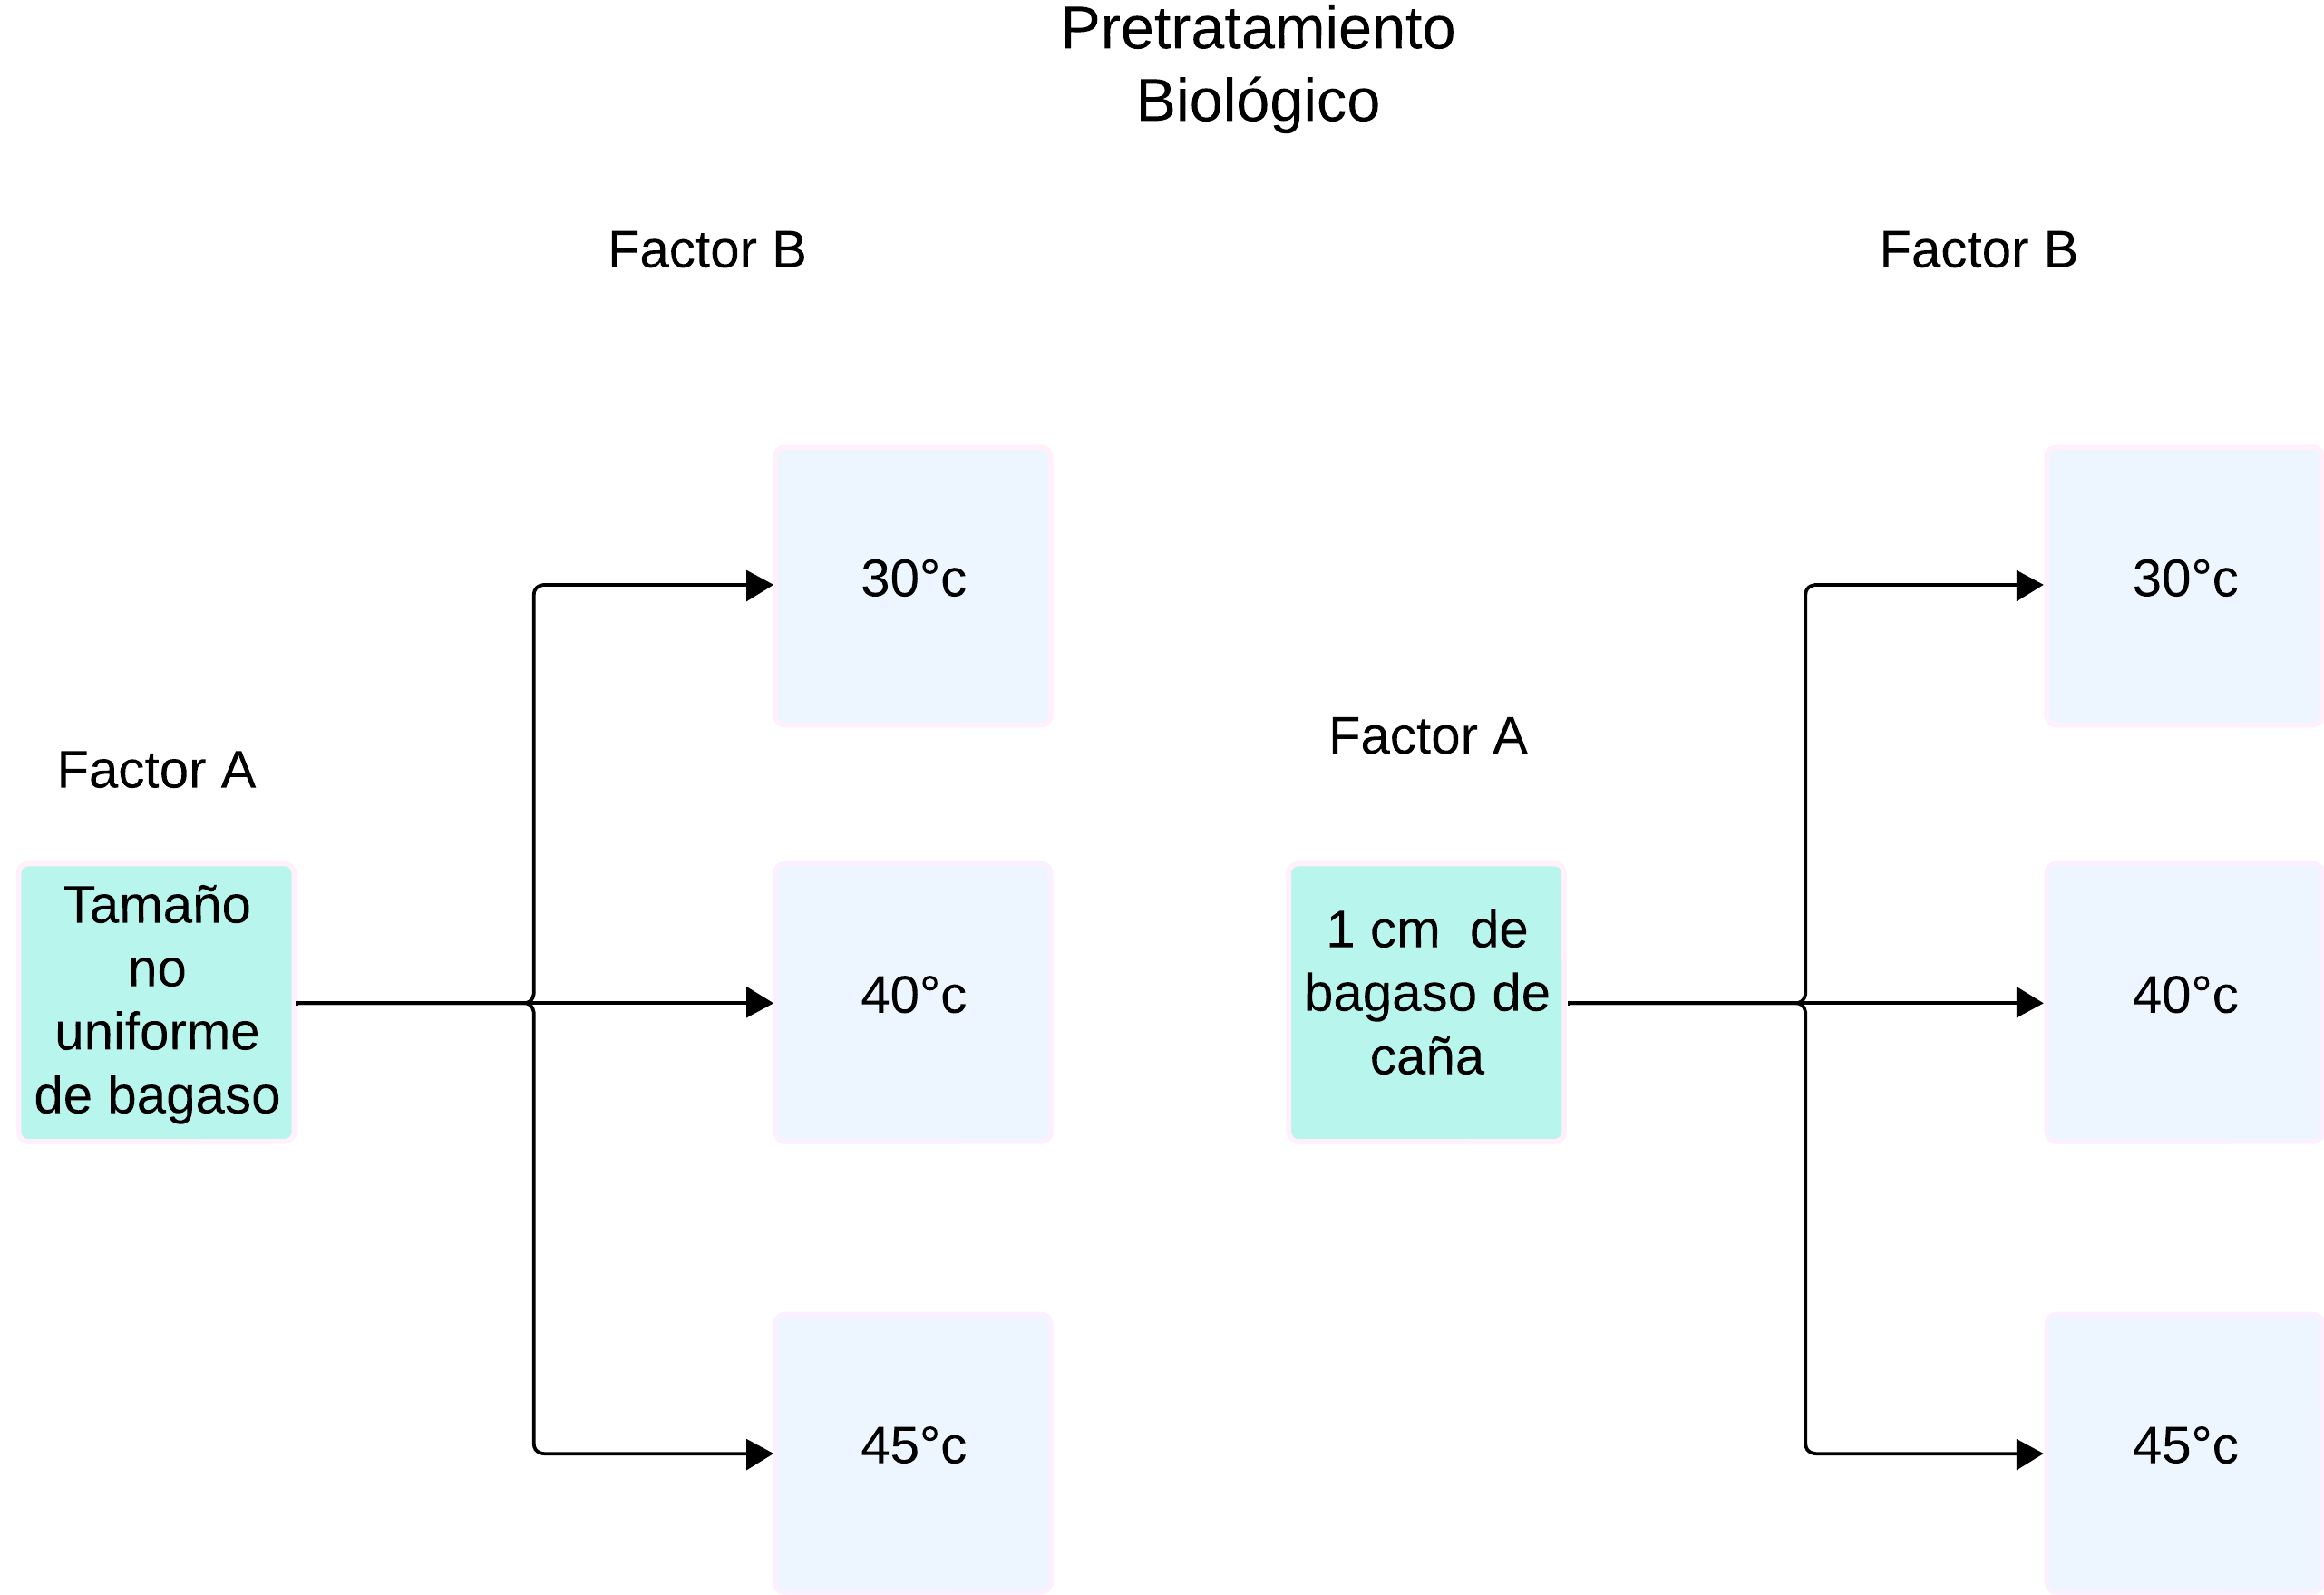
\includegraphics[width=0.7\linewidth]{imagenes/diagrama biologico}
			\caption{Diagrama de los pretratamientos}
			\label{Diagrama biologico}
		\end{figure}
		
		
	%%%%%%%%%%%%%%%%%%%%%%%%%%%%%%%%%%%%%%%%%%%%%%%%%%%%%%%%%%%%%%%%%%%%%%%%%%%%%%%%%%%%%%%%%%%%%%%%%%%%%%%%%%%%%%%%%%%%%%%%%%%%%%%%%%%%%%%%%%%%%%%%%%%%%%%%%%%%%%%%%%%%%%%%%%%%%%%%%
		
		
		
	
		
	\subsubsection{ Diseño experimental del pretratamiento Alcalino}
	\label{Diseño factorial del pretratamiento alcalino}

Para el caso del pretratamiento alcalino con hidróxido de sodio las temperaturas que se trabajaran son a 80 °C, 90 °C y 95 °C para observar el comportamiento del porcentaje de bioetanol si trabajamos con valores cercanos al mencionado, así como modificar el tamaño de bagazo, esto para saber el impacto del tamaño de biomasa al moverlo en el reactor tipo Batch (por lotes).
En la Tabla \ref{tab:Variablesalcalino} se mencionan las cantidades por insumo que se utilizaran para las pruebas con pretratamiento alcalino. Se menciona el tiempo de pretratamiento, siendo este una de las variables que se modificaran en las pruebas. El mezclado del reactivo es importante dado que nos ayuda a mantener la mezcla y la temperatura homogénea dentro del reactor tipo Batch, por lo que en la Tabla también menciona las condiciones de mezclado.


	\begin{table}[H]
	\centering
	\caption{Condiciones de operación fijas del reactor  para el pretratamiento biologico del bagazo de caña.}
	\label{tab:Variablesalcalino}
	\resizebox{\textwidth}{!}{
		\begin{tabular}{| c | c | c | c | c | c |      }
			\hline
			\textbf{Cantidad de} & \textbf{Cantidad de} & \textbf{Volumen de la carga} & \textbf{Tiempo del pretratamiento} & \multicolumn{2}{c|}{ \textbf{Condiciones de agitación} } \\  
			\textbf{bagazo de caña} & \textbf{humus de lombriz} & \textbf{ } & \textbf{Carga de humus} & \multicolumn{2}{c|}{  }  \\  
			\hline
			
			\multirow{5}{*}{4 \% p/v } & \multirow{5}{*}{2\% p/v }  & \multirow{6}{*}{6 l} & \multirow{3}{*}{5400} & \multirow{6}{*}{ 10 s encendido/apagado} & \multirow{6}{*}{142 RPM}  \\ 
			& & & &  &  \\ 
			& & & &  &   \\ 
			\cline{4-4}
			180 g& 300 g &  & \multirow{3}{*}{7870} &  & \\
			& & & & &   \\
			& & & &  &  \\ 
			\hline
		\end{tabular}
	}
\end{table}




De la misma forma cada pretratamiento sera realizado con tres factores, el factor A es el tamaño de partícula, es decir TNUB y 1 cm; para factor B es la temperatura donde tiene tres niveles modificando a 95°c , 90°c, 80°c, y por ultimo el factor c o el tercero factor que tiene dos niveles (5400 s o 7870 s). En total se realizaran 12 experimentaciones para el pretratamiento alcalino, como se muestra en la Tabla \ref{alcalino}. Esta presenta en la segunda columna el factor A, es decir el tamaño de bagazo a considerar en la experimentación, para la tercera columna se muestra la temperatura en las que se realizaran las experimentaciones, es decir el factor B.

\begin{table}[H]
	\centering
	\caption{Condiciones de operación del reactor para la producción de bioetanol 2G con pretratamiento biológico. Diseño de experimentos}
	\label{alcalino}
	\begin{tabular}{|c|c|c|  }
		\hline
		\textbf{Num de} & \textbf{Tamaño de particula } & \textbf{Temperatura} \\
	\textbf{experimento}	& \textbf{ del bagazo de caña} &   \textbf{(°C )}  \\		
		\hline
		1   & \multirow{3}{*}{TNUB*} & 95  \\	\cline{1-1}	
		2 &  & 90 \\ \cline{1-1} 						
		3 &  & 80 \\ \cline{1-3}			
		4 &\multirow{3}{*}{1 cm} & 95    \\\cline{1-1}			
		5 &  & 90   \\  \cline{1-1}				
		6 &  & 80     \\  \cline{1-1}		
		\hline
	\end{tabular}
		\\[3 pt] % Espacio adicional
% {\raggedright \footnotesize $^{*}$Tamaño no uniforme de bagazo. \par}
\footnotesize{$^{*}$  Tamaño no uniforme de bagazo.}
\end{table}





A continuación se presenta un diagrama donde se clasifica por factores cada variable a considerar, esto solo para el caso del pretratamiento alcalino, ver figura  \ref{Diagrama1}.



\begin{figure} [H]
	\centering
	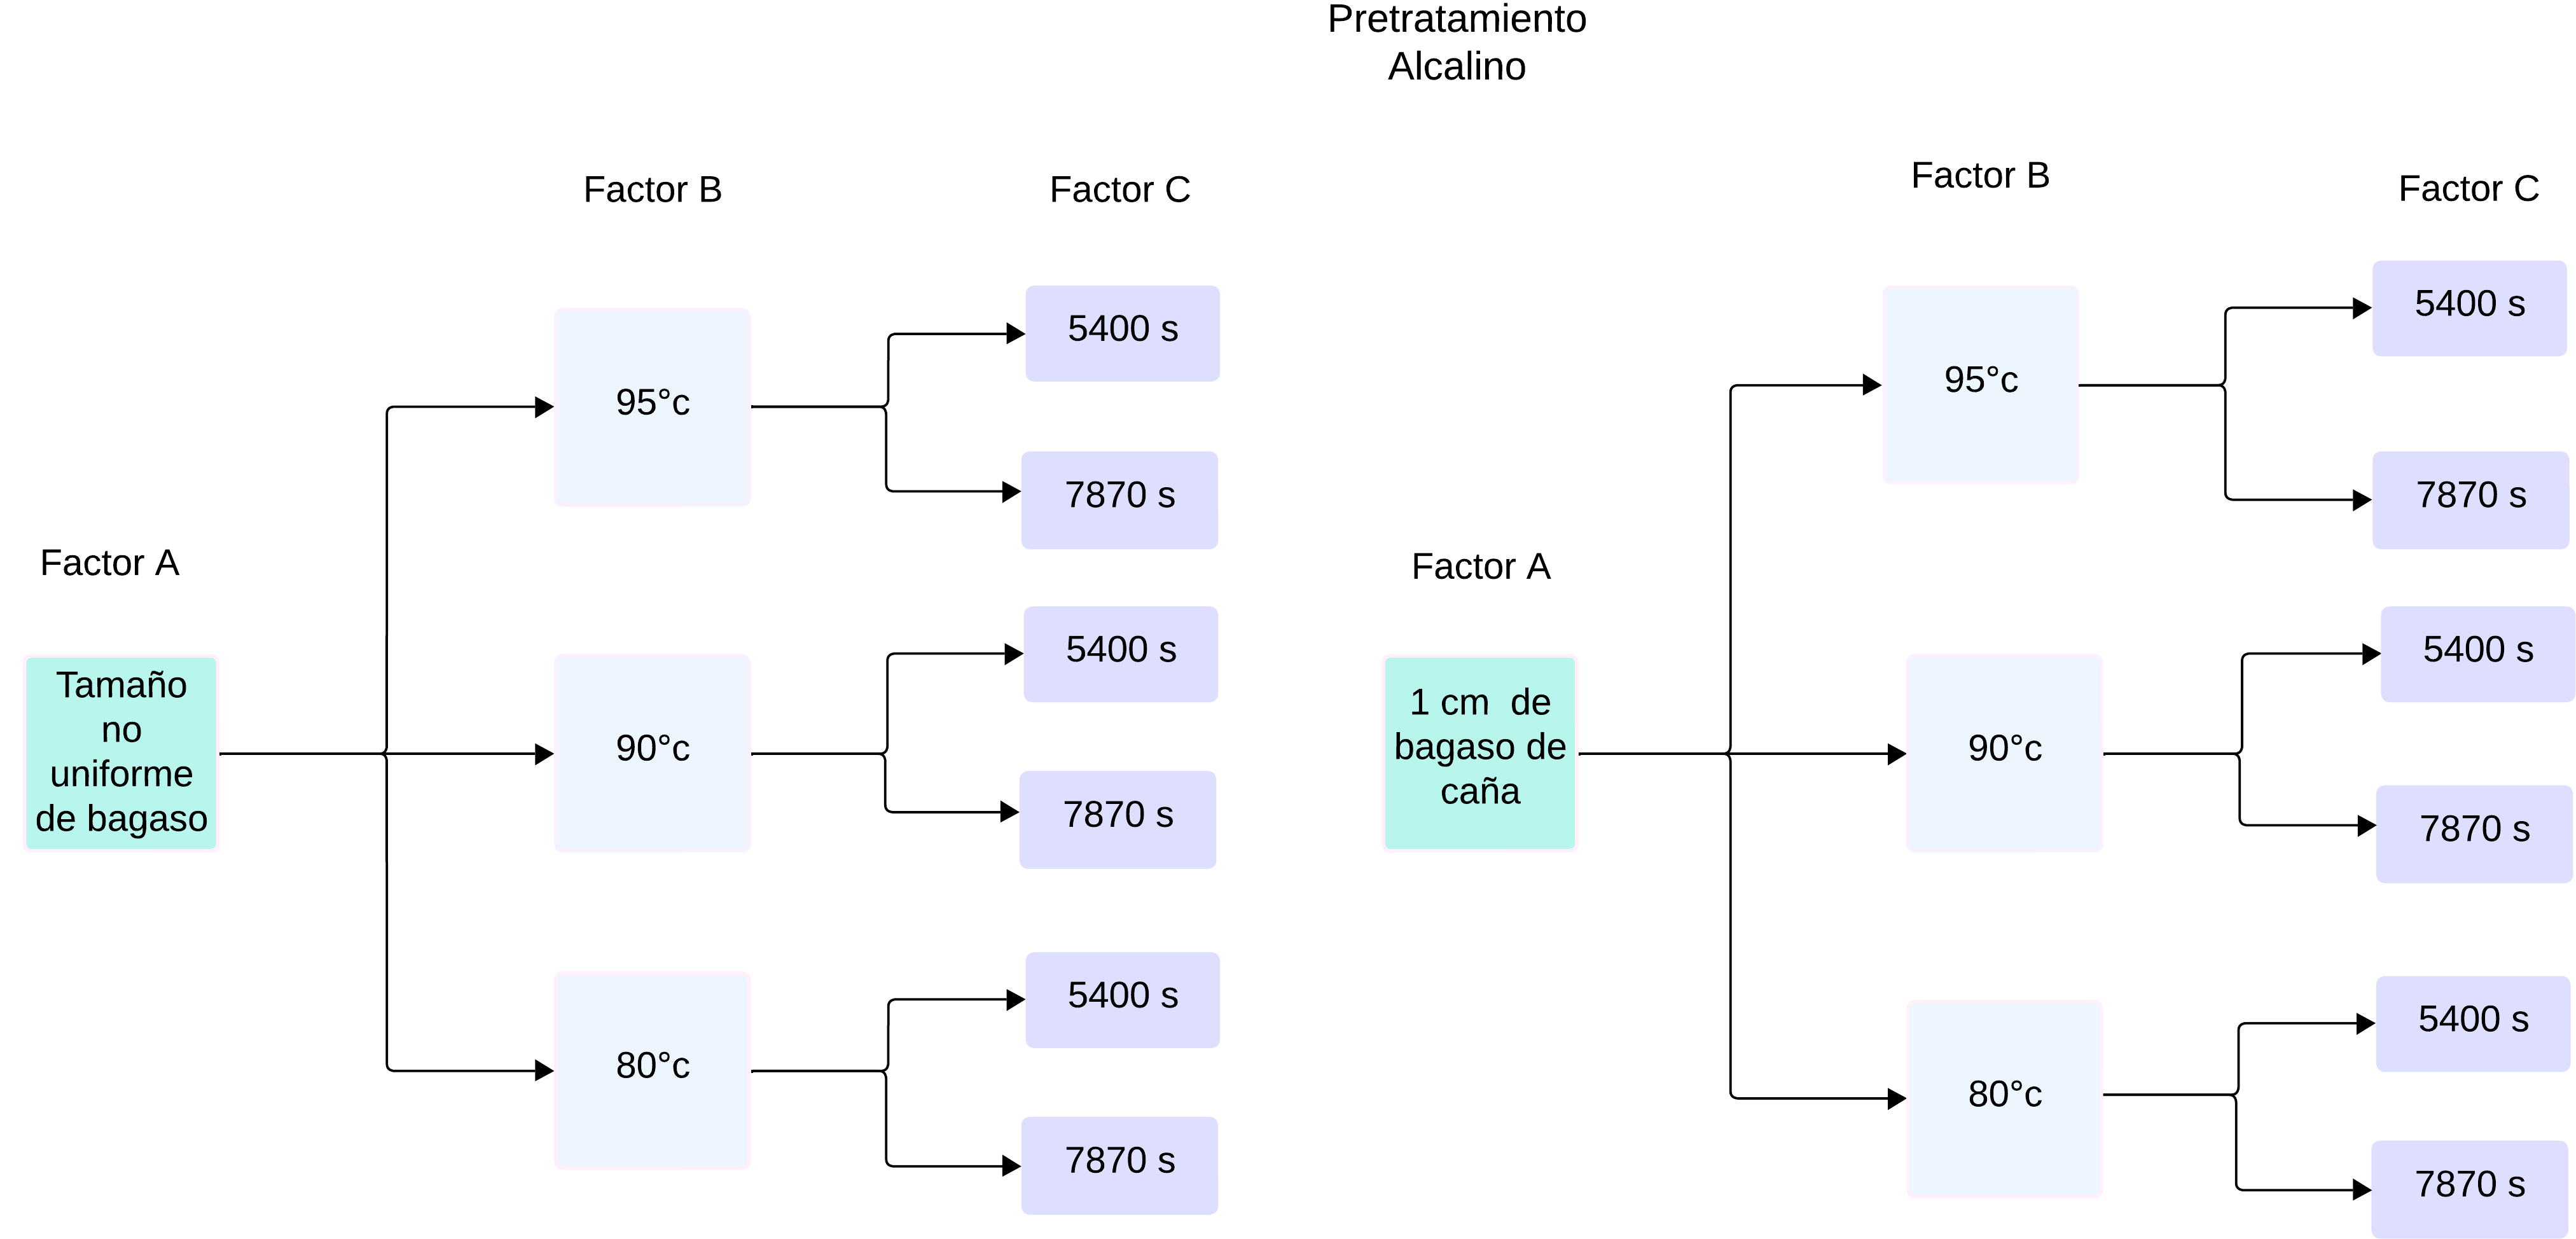
\includegraphics[width=0.9\linewidth]{imagenes/Diagrama alcalino}
	\caption{Diagrama de los pretratamientos}
	\label{Diagrama1}
\end{figure}



%%%%%%%%%%%%%%%%%%%%%%%%%%%%%%%%%%%%%%%%%%%%%%%%%%%%%%%%%%%%%%%%%%%%%%%%%%%%%%%%%%%%%%%%%%%%%%%%%%%%%%%%%%%%%%%%%%%


%\singlespacing
	
		\subsubsection{Diseño de experimentos para la configuración:
			sacarificación y fermentación simultaneas (SSF)}
		\label{SacariSF}	
		
%		\onehalfspacing
		
		Por otra parte, tenemos la configuración para la producción de bioetanol, donde tomando como referencia la tesis \cite{Arturo2022evaluacion}, se pueden tener los valores para los insumos en la configuración SSF, en donde intervienen los elementos como la carga de biomasa que es la cantidad de bagazo previamente pretratado con alguno de los métodos anteriores, levadura necesaria para una buena fermentación, el ph de la solución dentro del reactor, la carga enzimática que es uno de los elementos importantes para realizar la hidrólisis y por ultimo la temperatura del la hidrólisis y fermentación en etapas conjuntas. En la Tabla 	\ref{tab:Variables a modificar para la hidrolisis y fermentacion}, muestran los valores de cada uno de los elementos a tomar en consideración para la la configuración de etapas juntas (SSF). \\[0.5em]
		
		\begin{table} [h!]
			\centering
			\caption{Variables a modificar en la hidrólisis y fermentación}
			\label{tab:Variables a modificar para la hidrolisis y fermentacion}
			\small
			\resizebox{17cm}{!} {
			\begin{tabular}{|c|c|c|c|c|c|c|c|c|}
				\hline
			\textbf{Biomasa}  &\textbf{ Volumen}  & \textbf{Carga de } & \textbf{Carga}  & \textbf{Inoculo}  &\textbf{ Ph}  & \textbf{Temperatura } & \textbf{Tiempo}   \\
				 &   & \textbf{ biomasa}  & \textbf{enzimática } & \textbf{de levadura } & &  &     \\
				
				\hline
			\multirow{2}{*}{Bagazo de caña} &\multirow{2}{*}{2 l}  &\multirow{2}{*}{5\%}  & \multirow{2}{*}{20 UPF/g } & \multirow{2}{*}{10\% } &\multirow{2}{*}{ 5} & \multirow{2}{*}{43 °c} & \multirow{2}{*}{48h }   \\
			  &   & & &  &  & &     \\		
				\hline
			\end{tabular}}
		\end{table}
		
		
		
		
		
		

		
		Se puede observar que se utilizan dos volumen, ya que uno 3600 ml es utilizando biomasa pretratada con humus de lombriz, es decir realizando un pretratamiento biológico, y para el caso del volumen de 5.5 l es utilizando biomasa pretratada con hidróxido de sodio, también llamado pretratamiento alcalino.
		
		
			\begin{itemize}
			\item  Carga enzimática
	     	\end{itemize}
		
		
	La carga enzimática se refiere a la relación de porcentaje entre el peso de soluto y volumen de solución. En la ecuación \ref{carga} se muestras la obtención de la carga enzimática en ml, donde utiliza las unidades de papel filtro (UPF) la cual es una medida de laboratorio para medir las enzimas y por ultimo utiliza el valor constante de 3.7 (\cite{Arturo2022evaluacion}).
			
	\begin{equation}
		\label{carga}
		\text{carga enzimática (ml)} = \frac{3.7}{UPF}
	\end{equation}
	

	
		

	%%%%%%%%%%%%%%%%%%%%%%%%%%%%%%%%%%%%%%%%%%%%%%%%%%%%%%%%%%%%%%%%%%%%%%%%%%%%%%%%%%%%%%%%%%%%%%%%%%%%%%%%%%%%%%%%%%%%%%%%%%%%%%%%%%%%%%%%%%%%%%%%%%%%
			
			
	
			\subsection{Implementación}

			Para las pruebas experimentales tendremos en cuenta de primera instancia los materiales necesarios en cada pretratamiento, posteriormente se menciona los pasos que conlleva realizar cada prueba de experimentación.
			

			\subsubsection{Pre-Pretratamiento}

			
			El pre-pretratamiento ayuda clasificar el tamaño de bagazo que se va a utilizar, así como secar el bagazo en caso de tener humedad. El material y compuestos para poder limpiar y clasificar el tamaño de bagazo se menciona a continuación.
			\\[0.5em]
			\textbf{Compuestos} 
			\begin{itemize}[label=\textcolor{blue}{$\bullet$}]
			 \item	\textit{ Bagazo de caña }
			\end{itemize} 
			
			
			\textbf{Materiales} \\[0.5em]
			
			
			\begin{tabular}{p{0.3\textwidth}p{0.3\textwidth}p{0.3\textwidth}}
			\textit{	$\bullet$ Lona} &  \textit{$\bullet$  Malla cuadrada 1 cm} & \textit{$\bullet$ Bolsa plástica  }\\
				&&\textit{de 30×40 cm} \\
				\textit{$\bullet$ Báscula} & \textit{$\bullet$ Cubeta con capacidad de 10 l} & 
			\end{tabular}
		\\[0.5em]
			
			
			\textbf{Procedimiento}
			\\[0.5em]
			\textbf{1.} Se implementa una barrera de protección mediante una lona impermeable extendida sobre el piso, evitando el contacto directo del bagazo de caña con superficies contaminantes. Sobre esta superficie aislante, se distribuye uniformemente el bagazo de caña, para facilitar el secado pasivo y la eliminación controlada de su humedad residual, proceso documentado en la Figura \ref{secado1}

			
			\textbf{2.}	La clasificación por tamaño se efectuó usando un arreglo de dos mallas metálicas de 1 cm, montadas en serie sobre un recipiente de 10 L. Mediante agitación rítmica del bagazo colocado en la malla superior (Figura \ref{cernir_bagazo_B}), las fracciones menores a 1 cm fueron seleccionadas por gravedad hacia la cubeta, mientras que las partículas mayores se retuvieron en el tamiz.
		
			
				\begin{figure}[H]
				\centering
				\begin{minipage}{0.46\textwidth}
					\centering
					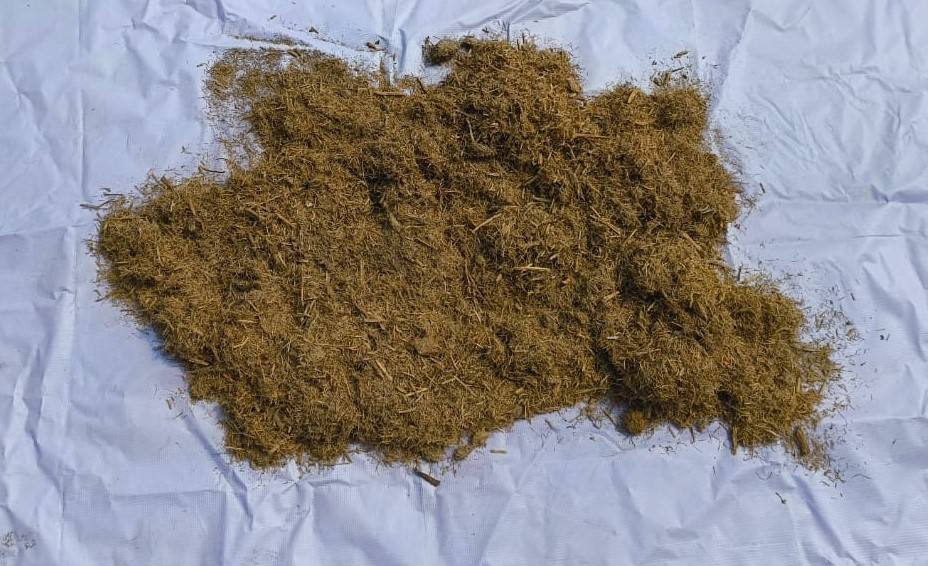
\includegraphics[width=5cm, height=3cm]{imagenes/secado de bagazo} % Cambia "imagen1.jpg" por el nombre de tu archivo
					\caption{Bagazo de caña tendido sobre una lona.}
					\label{secado1}
				\end{minipage}
				\hfill
				\begin{minipage}{0.48\textwidth}
					\centering
					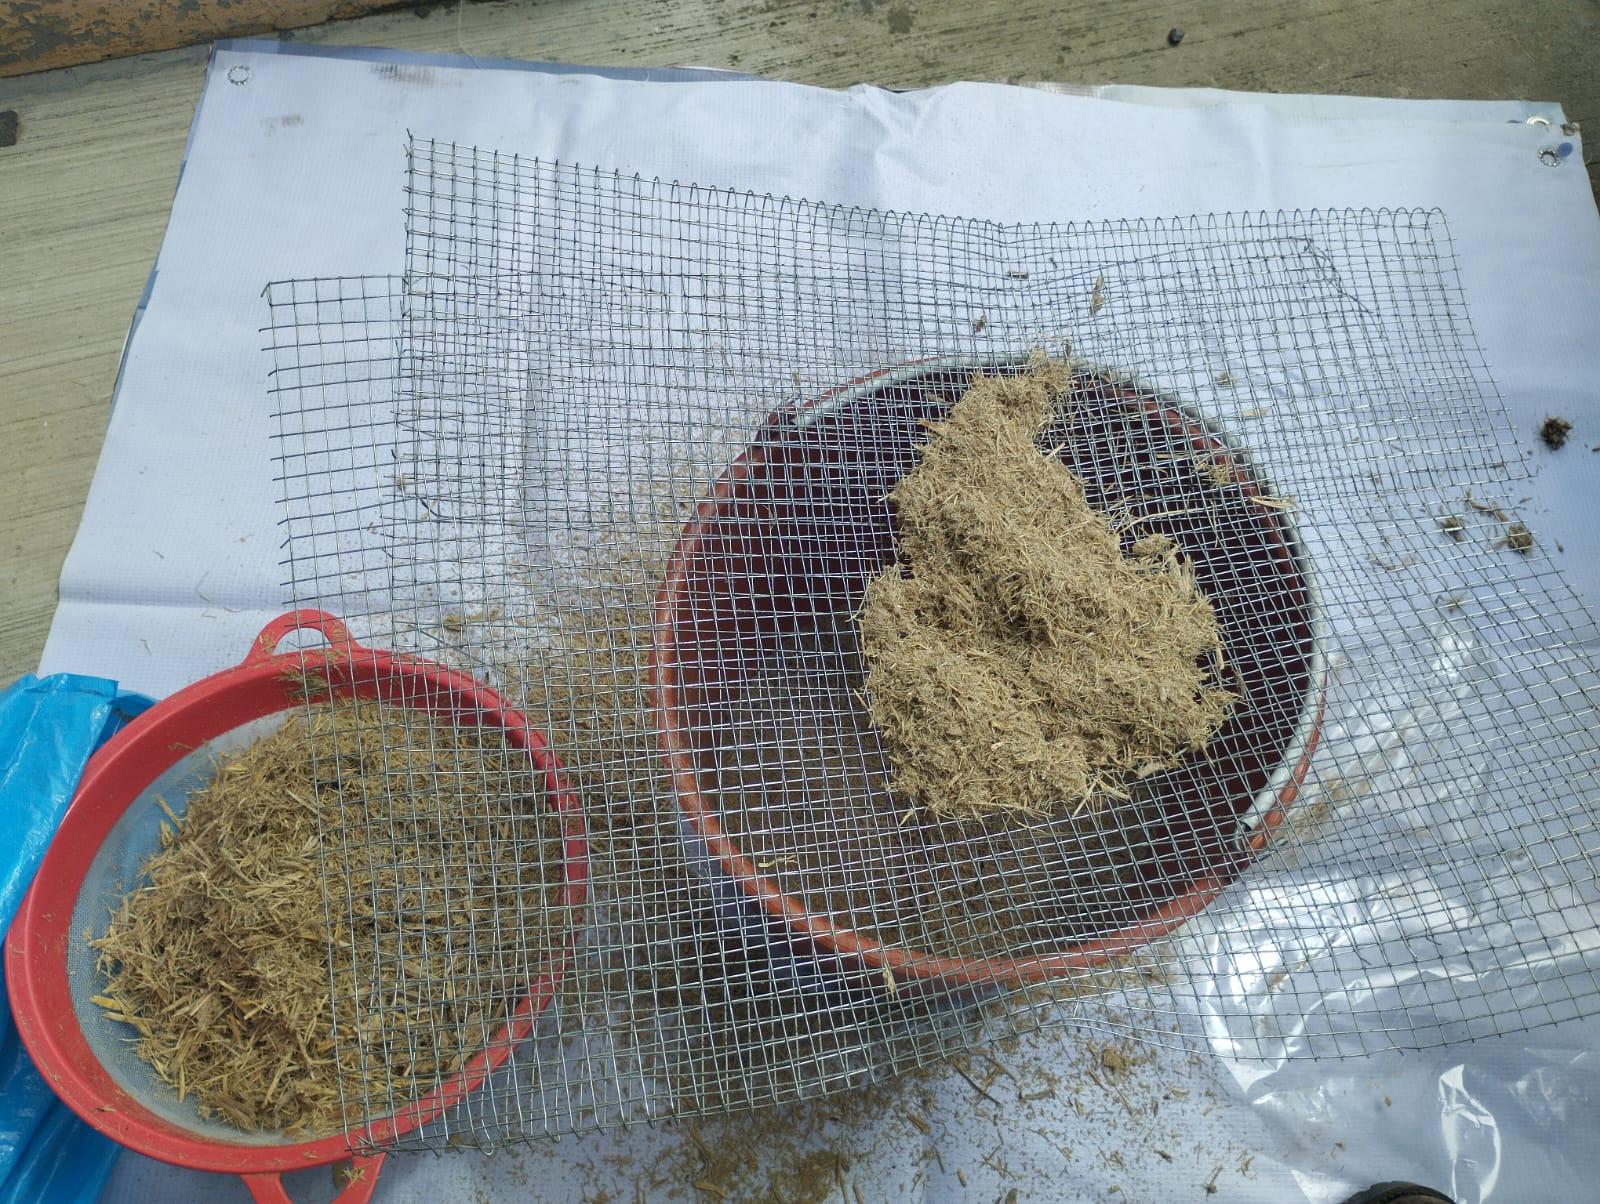
\includegraphics[width=5cm, height=3cm]{imagenes/cernir_bagazo_1} % Cambia "imagen2.jpg" por el nombre de tu archivo
					\caption{El bagazo es cernido con ayuda de la malla de 1 cm.}
					\label{cernir_bagazo_B}
				\end{minipage}
			\end{figure}
			
			
			
			
			
			\textbf{3.}	El bagazo se somete a dos ciclos adicionales de cribado utilizando el mismo sistema de doble malla (abertura de 1 cm), aplicando un movimiento armónico controlado en cada repetición (Figura \ref{cernir_bagazo_2C}). Este proceso iterativo permite obtener una fracción de partículas con tamaño significativamente reducido, optimizando la homogeneidad del material resultante.
			
			
			\textbf{4.} Para garantizar un tamaño de partícula uniforme, el bagazo de caña se somete a un cribado adicional mediante un cedazo de malla más fina, con el objetivo de obtener un material final con una granulometría controlada de 1 cm, lo que optimiza su posterior aprovechamiento en procesos industriales.v	ER Figura \ref{cernir_bagazo_cedazo}.
		
		
			\begin{figure}[H]
			\centering
			\begin{minipage}{0.46\textwidth}
				\centering
			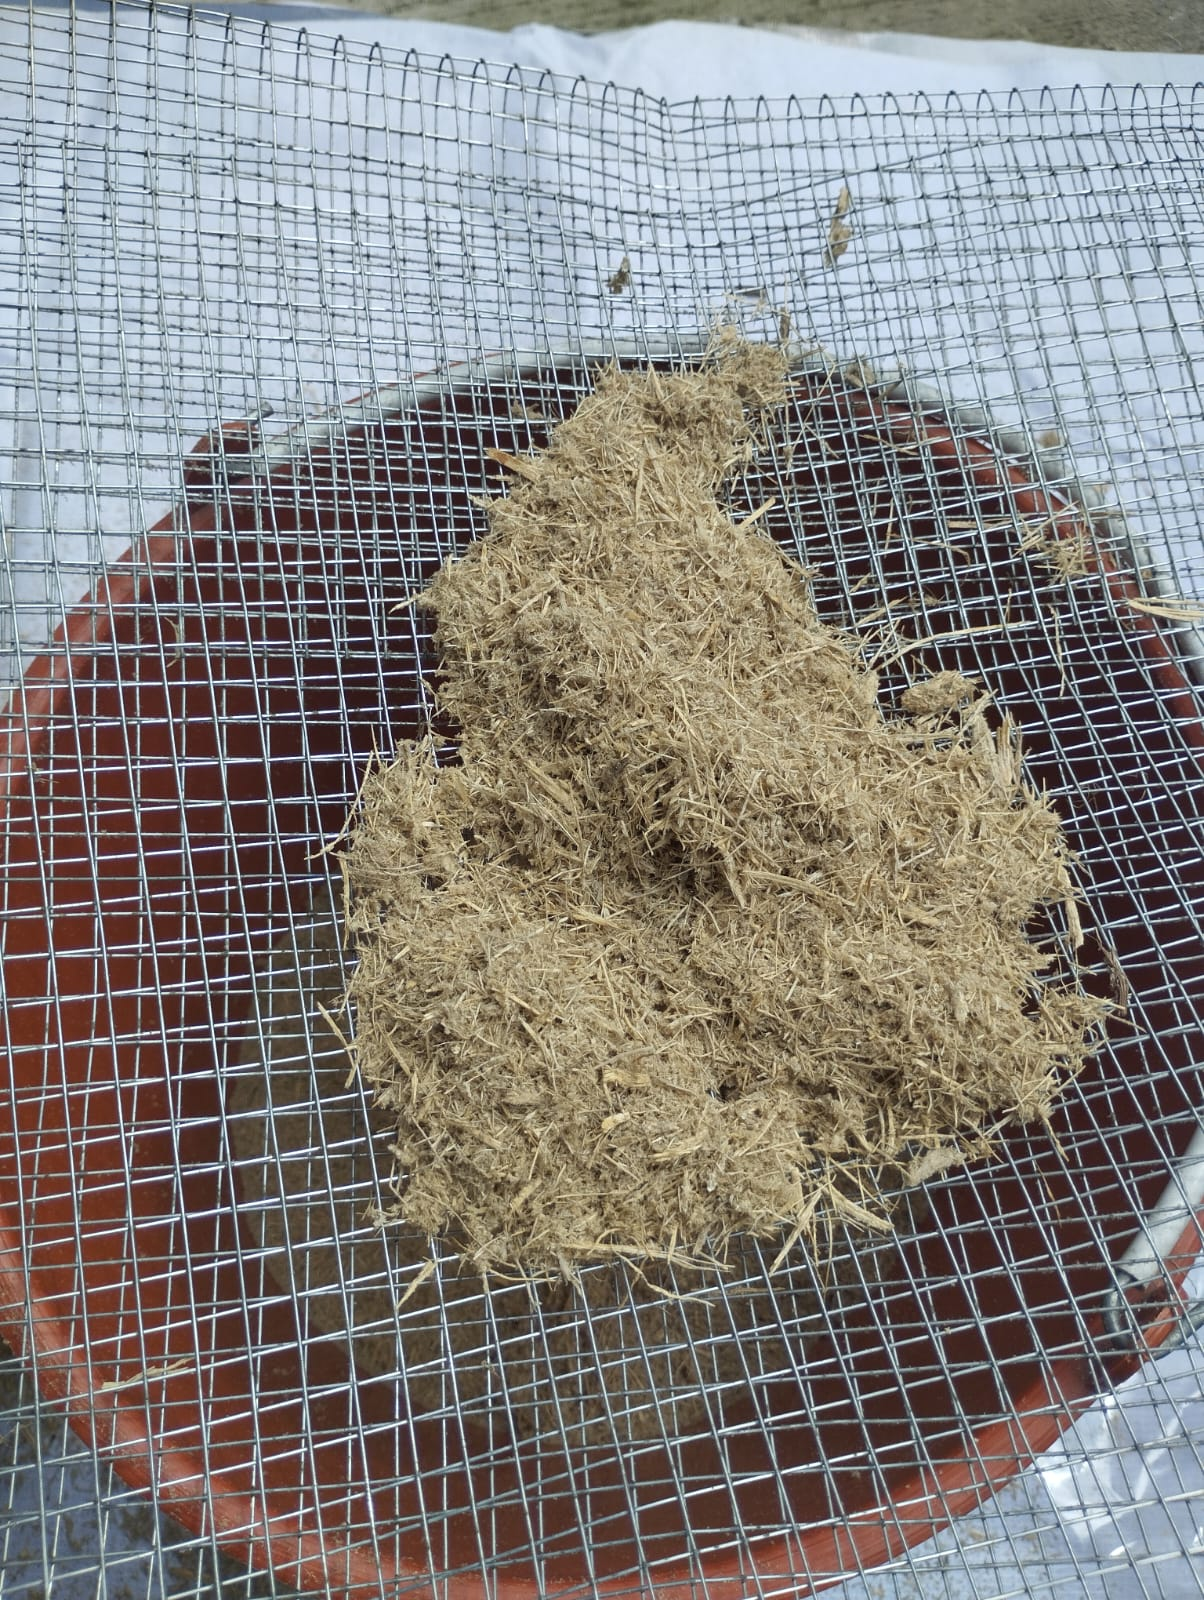
\includegraphics[width=\linewidth, height=4cm, keepaspectratio]{imagenes/cernir_bagazo_2}
			\caption{Momento donde el bagazo es clasificado}
			\label{cernir_bagazo_2C}
			\end{minipage}
			\hfill
			\begin{minipage}{0.48\textwidth}
				\centering
				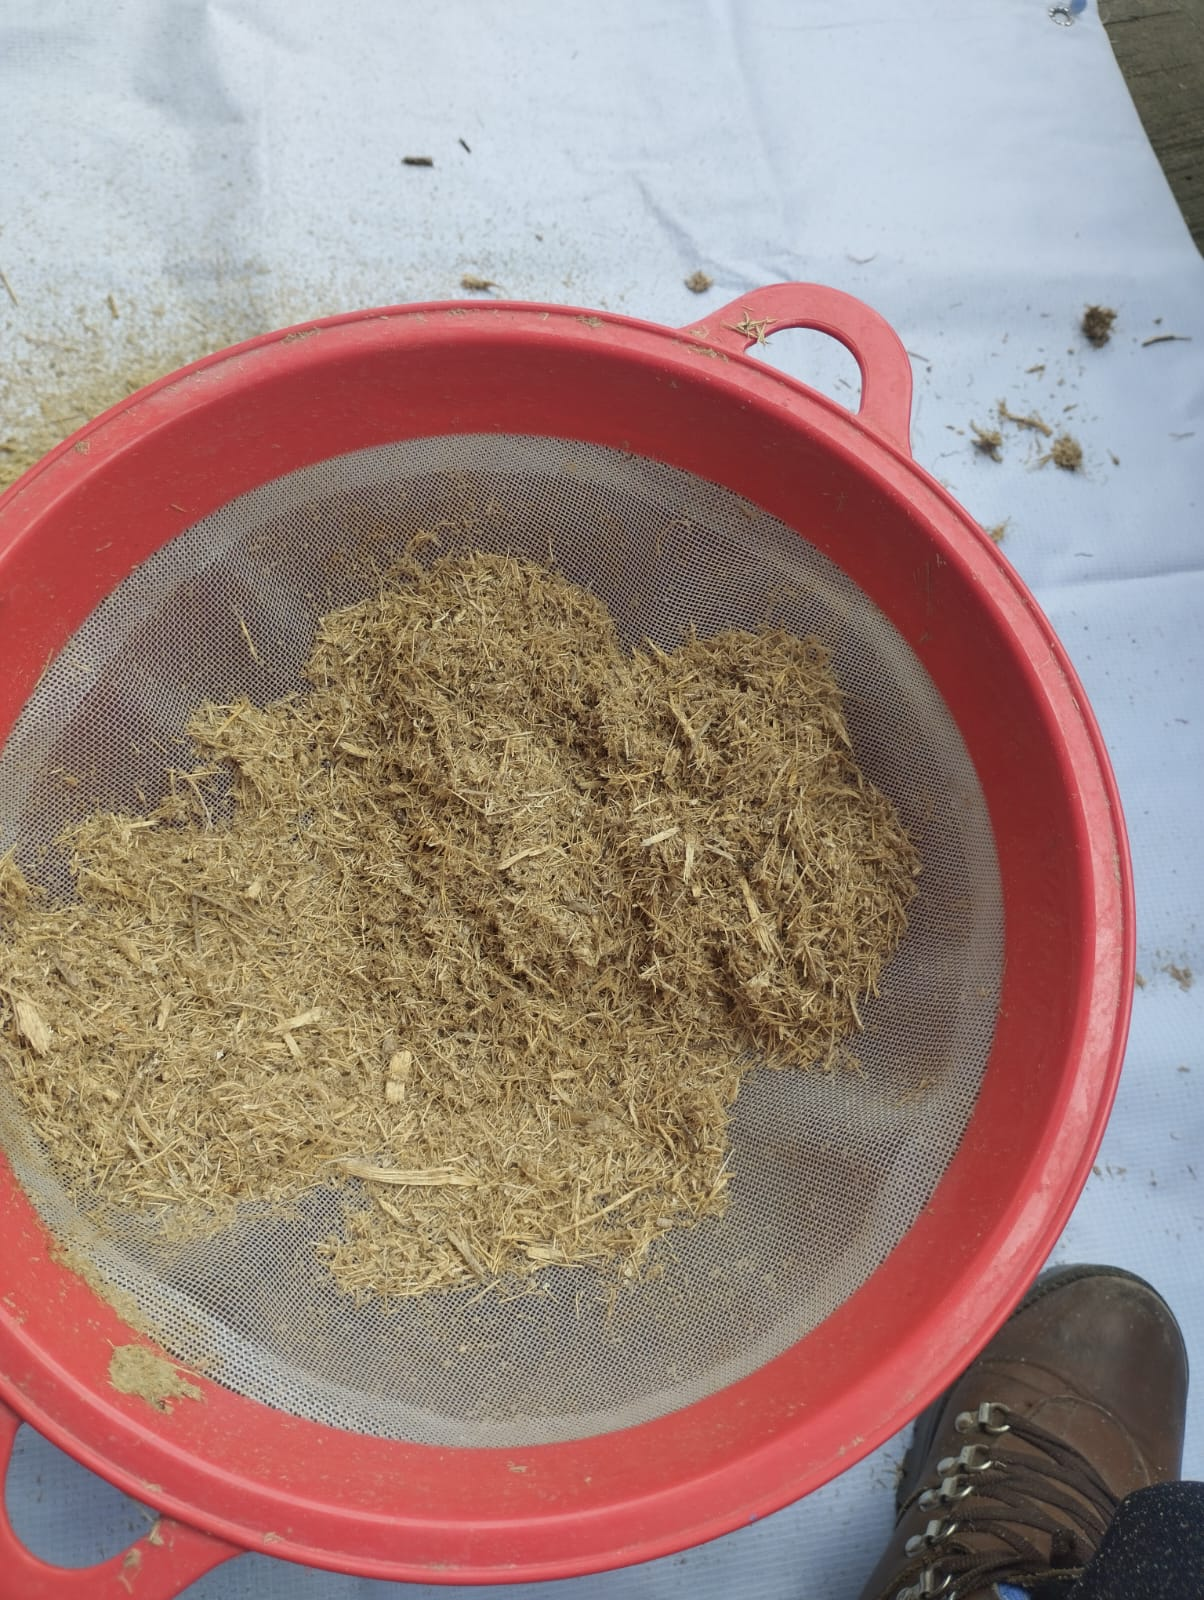
\includegraphics[width=\linewidth, height=4cm, keepaspectratio]{imagenes/cernir_bagazo_cedazo}
				\caption{Clasificación con colador para trozos grandes}
				\label{cernir_bagazo_cedazo}
			\end{minipage}
		\end{figure}
		
	
			\textbf{5.} El bagazo cernido se pesa en una báscula hasta alcanzar la masa requerida (240 g o 180 g, según el pretratamiento asignado) y posteriormente se introduce en una bolsa de plástico, la cual se sella herméticamente para evitar alteraciones en su contenido de humedad durante el almacenamiento o transporte.
			
			
			\begin{figure} [H]
				\centering
				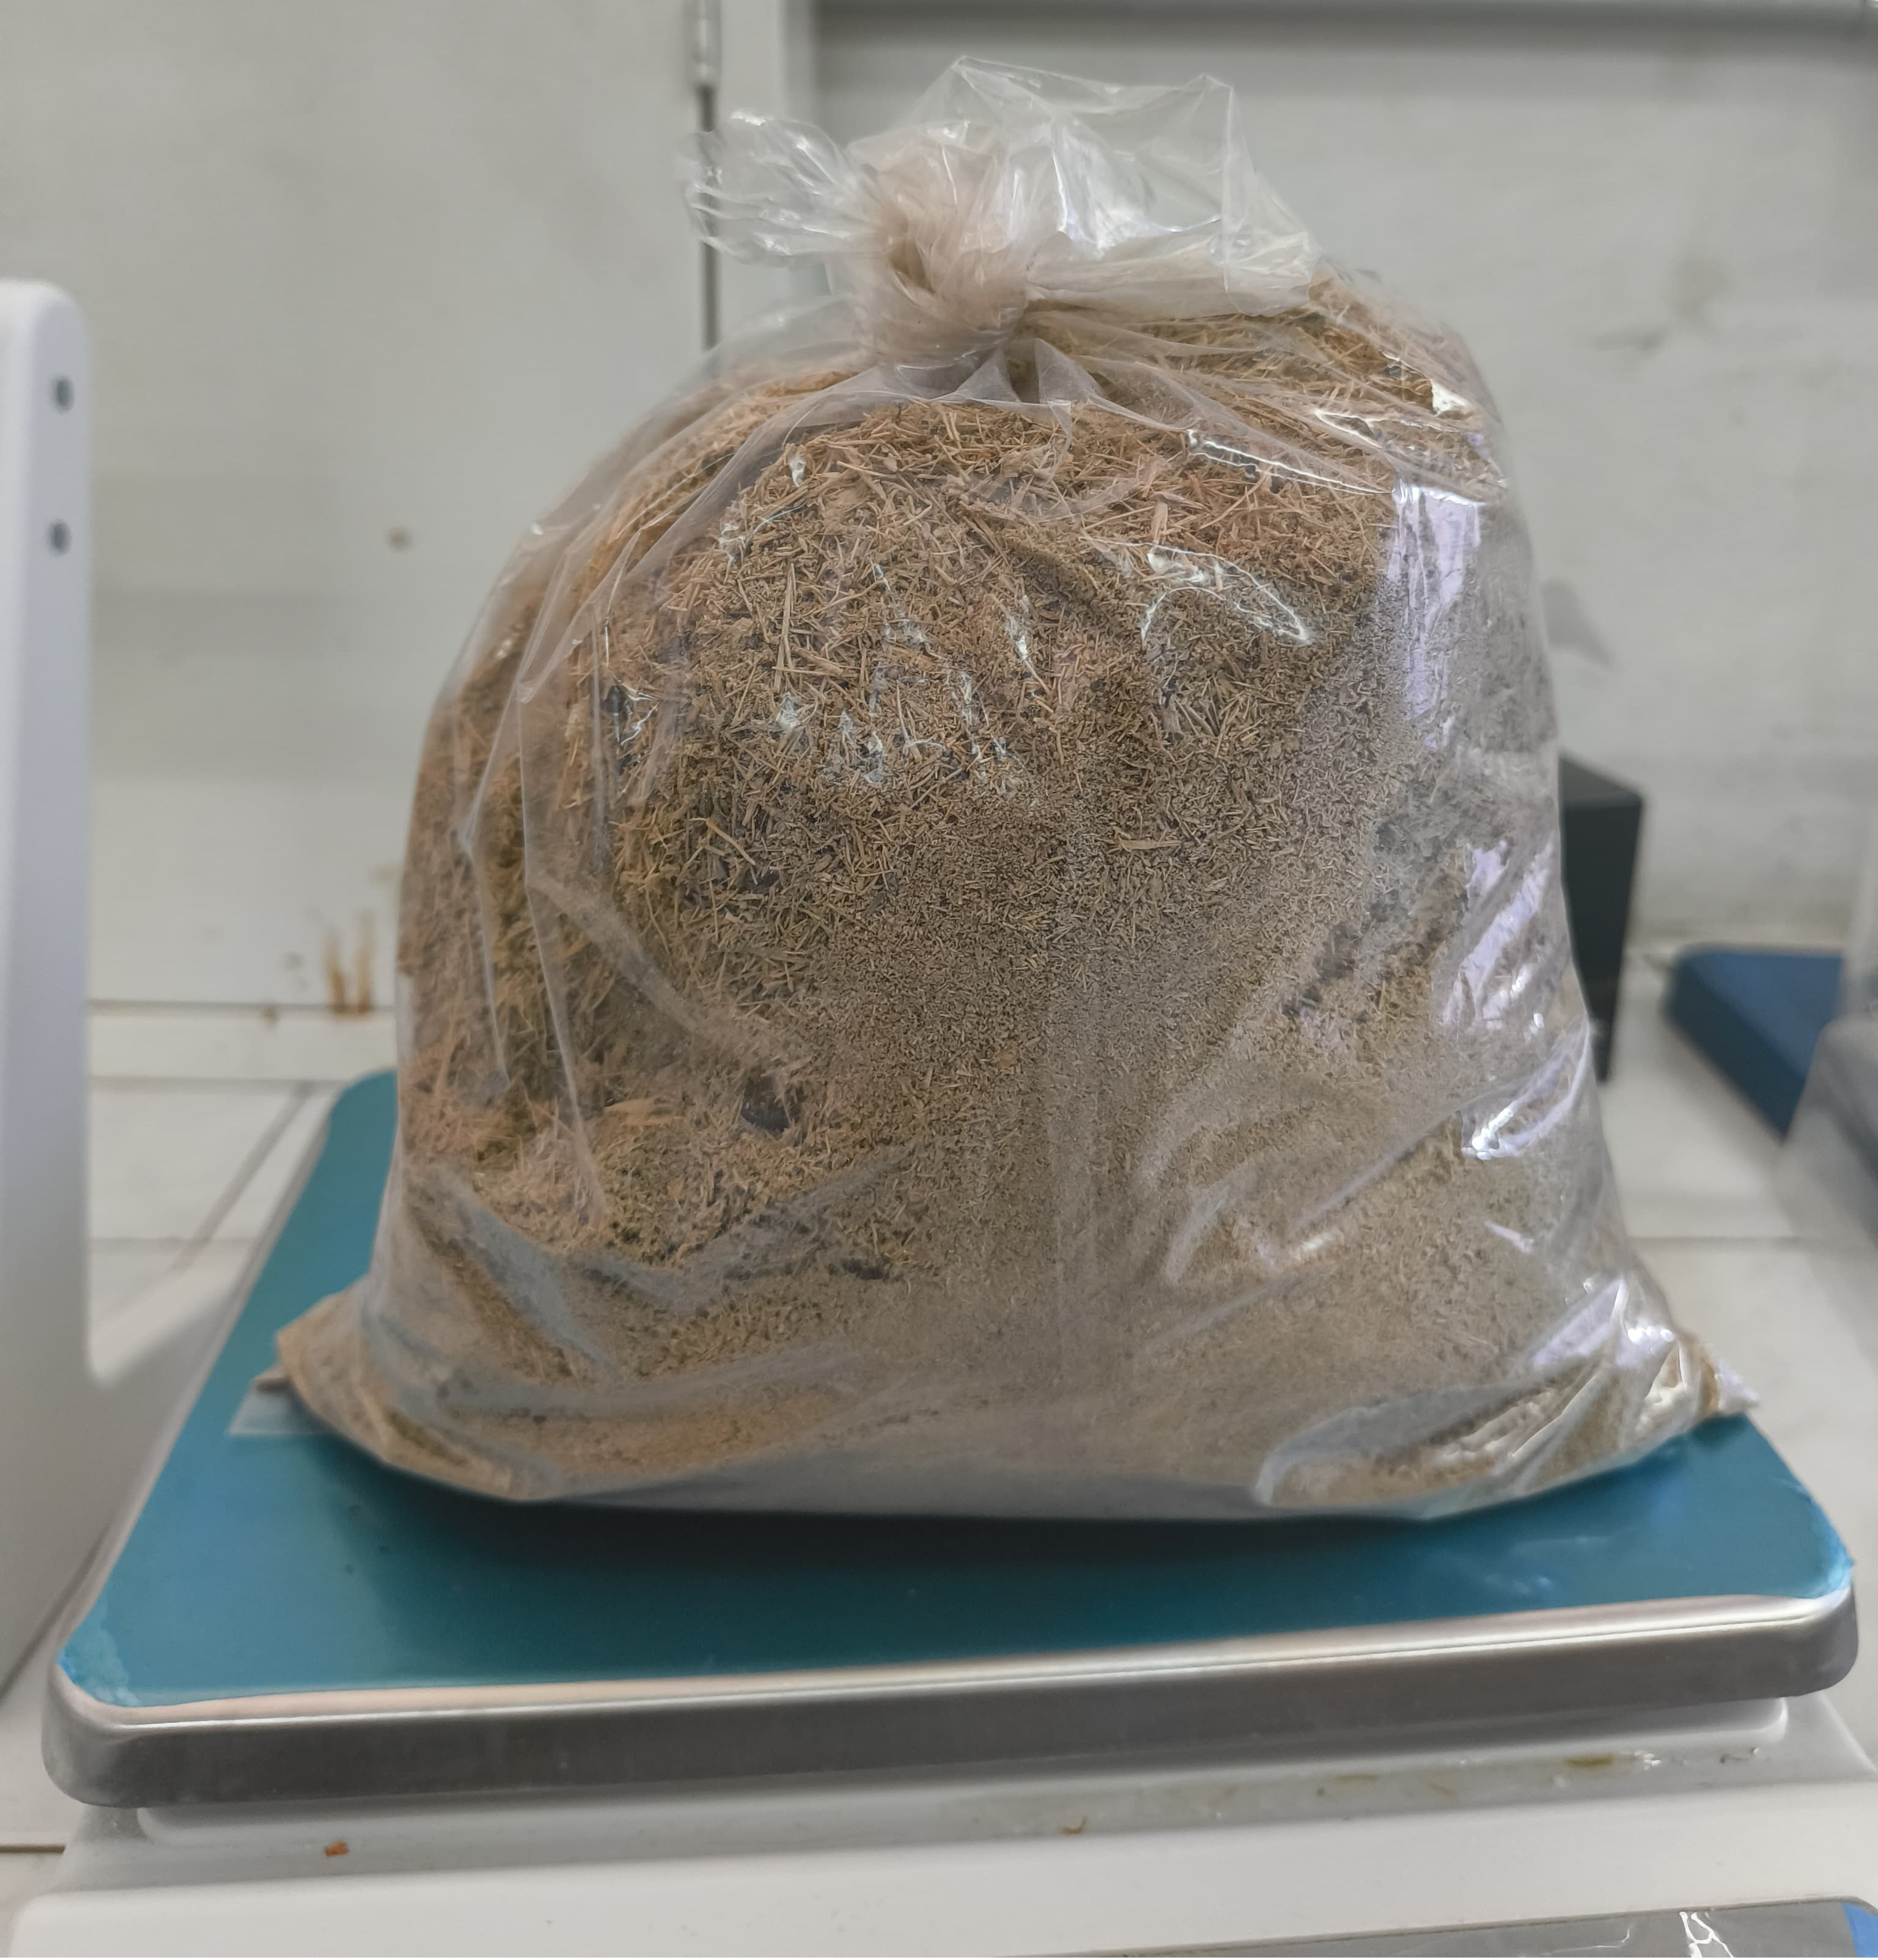
\includegraphics[width=5cm, height=3cm]{imagenes/cernir_bagazo_pesado}
				\caption{El bagazo cernido es colocado en la bolsa y es pesado.}
				\label{cernir_bagazo_pesado}
			\end{figure}
			
			
			%%%%%%%%%%%%%%%%%%%%%%%%%%%%%%%%%%%%%%%%%%%%%%%%%%%%%%%%%%%%%%%%%%%%%%%%%%%%%%%%%%%%%%%%%%%%%%%%%%%%%%%%%%%%%%%%%%%%%%%%%%%%%%%%%%%%%%%%%%%%%%%%%%%%%%%%%%%%%%%%
			
			
			\subsubsection{Pretratamiento Biológico}
	
			
		Para la ejecución del pretratamiento biológico, se requiere el siguiente conjunto de materiales y reactivos estandarizados. Posteriormente se mencionan los pasos para la experimentación.\\
			
			\textbf{Compuestos} \\[0.5em]
			

				\begin{tabular}{p{0.3\textwidth}p{0.3\textwidth}}
				\textcolor{blue}{$\bullet$} \textit{Humus de Lombriz}  &	\textcolor{blue}{$\bullet$} \textit{Bagazo de caña}
			\end{tabular} \\[0.5em]
			
			\textbf{Materiales} \\[0.5em] 
	
			\begin{tabular}{p{0.3\textwidth}p{0.3\textwidth}p{0.3\textwidth}}
				$\bullet$ \textit{Agua desmineralizada } & $\bullet$ \textit{Algodón} & $\bullet$ \textit{Bolsa plástica de 30×40 cm }\\
				$\bullet$ \textit{Báscula} & $\bullet$ \textit{Cinta aislante} & $\bullet$ \textit{Cinta de teflón}
			\end{tabular}
			\\[1em]
			
			
			\textbf{Procedimiento}
			\\[0.5em]
			\textbf{1.}	La dosificación del bagazo se realiza mediante pesaje con una báscula utilizando una bolsa plástica de 3 kg como recipiente, hasta alcanzar los 180 g requeridos. Este procedimiento aplica únicamente cuando no se emplea la medida estándar de 1 cm de longitud de partícula, en cuyo caso se utiliza directamente el material previamente clasificado y calibrado. Ver Figura \ref{bagazo_variostamaños}.
		
			
			\textbf{2.}	Mediante balanza analítica (±0.2 g) y material de vidrio calibrado (vaso de precipitado de 500 mL), se pesan exactamente 350 g de humus de lombriz grado técnico, siguiendo el procedimiento ilustrado en la Figura \ref{humus}.
			
			
				\begin{figure}[H]
				\centering
				\begin{minipage}{0.46\textwidth}
						\centering
					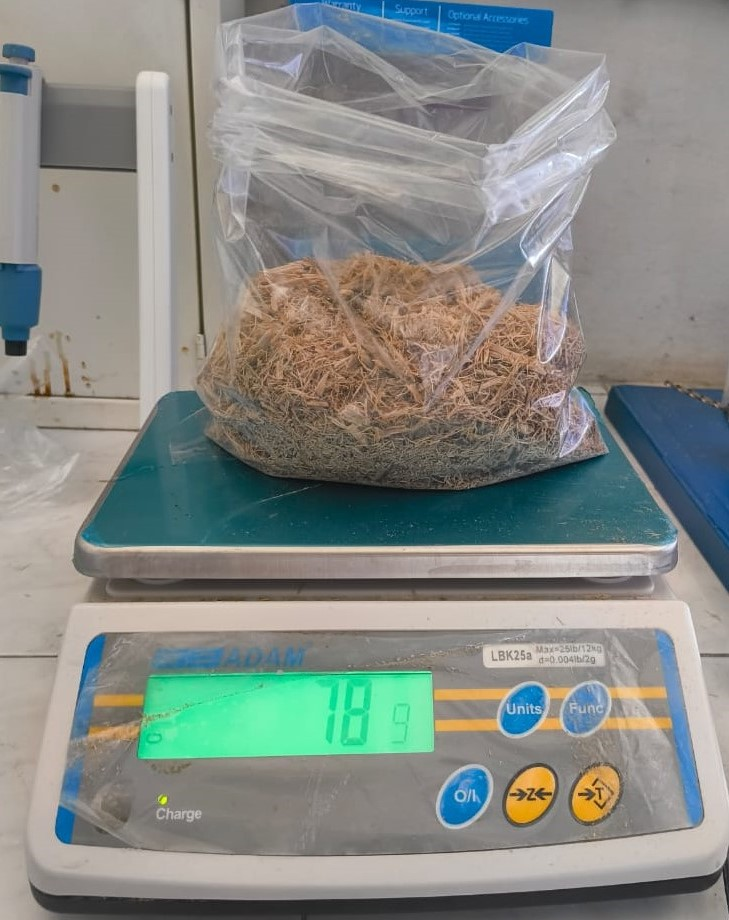
\includegraphics[width=3cm, height=5cm]{imagenes/pesado2}
					\caption{Fotografía muestra cuando se peso el bagazo de caña con medidas desde 1mm  hasta 10 cm aproximadamente.}
					\label{bagazo_variostamaños}
				\end{minipage}
				\hfill
				\begin{minipage}{0.48\textwidth}
				\centering
				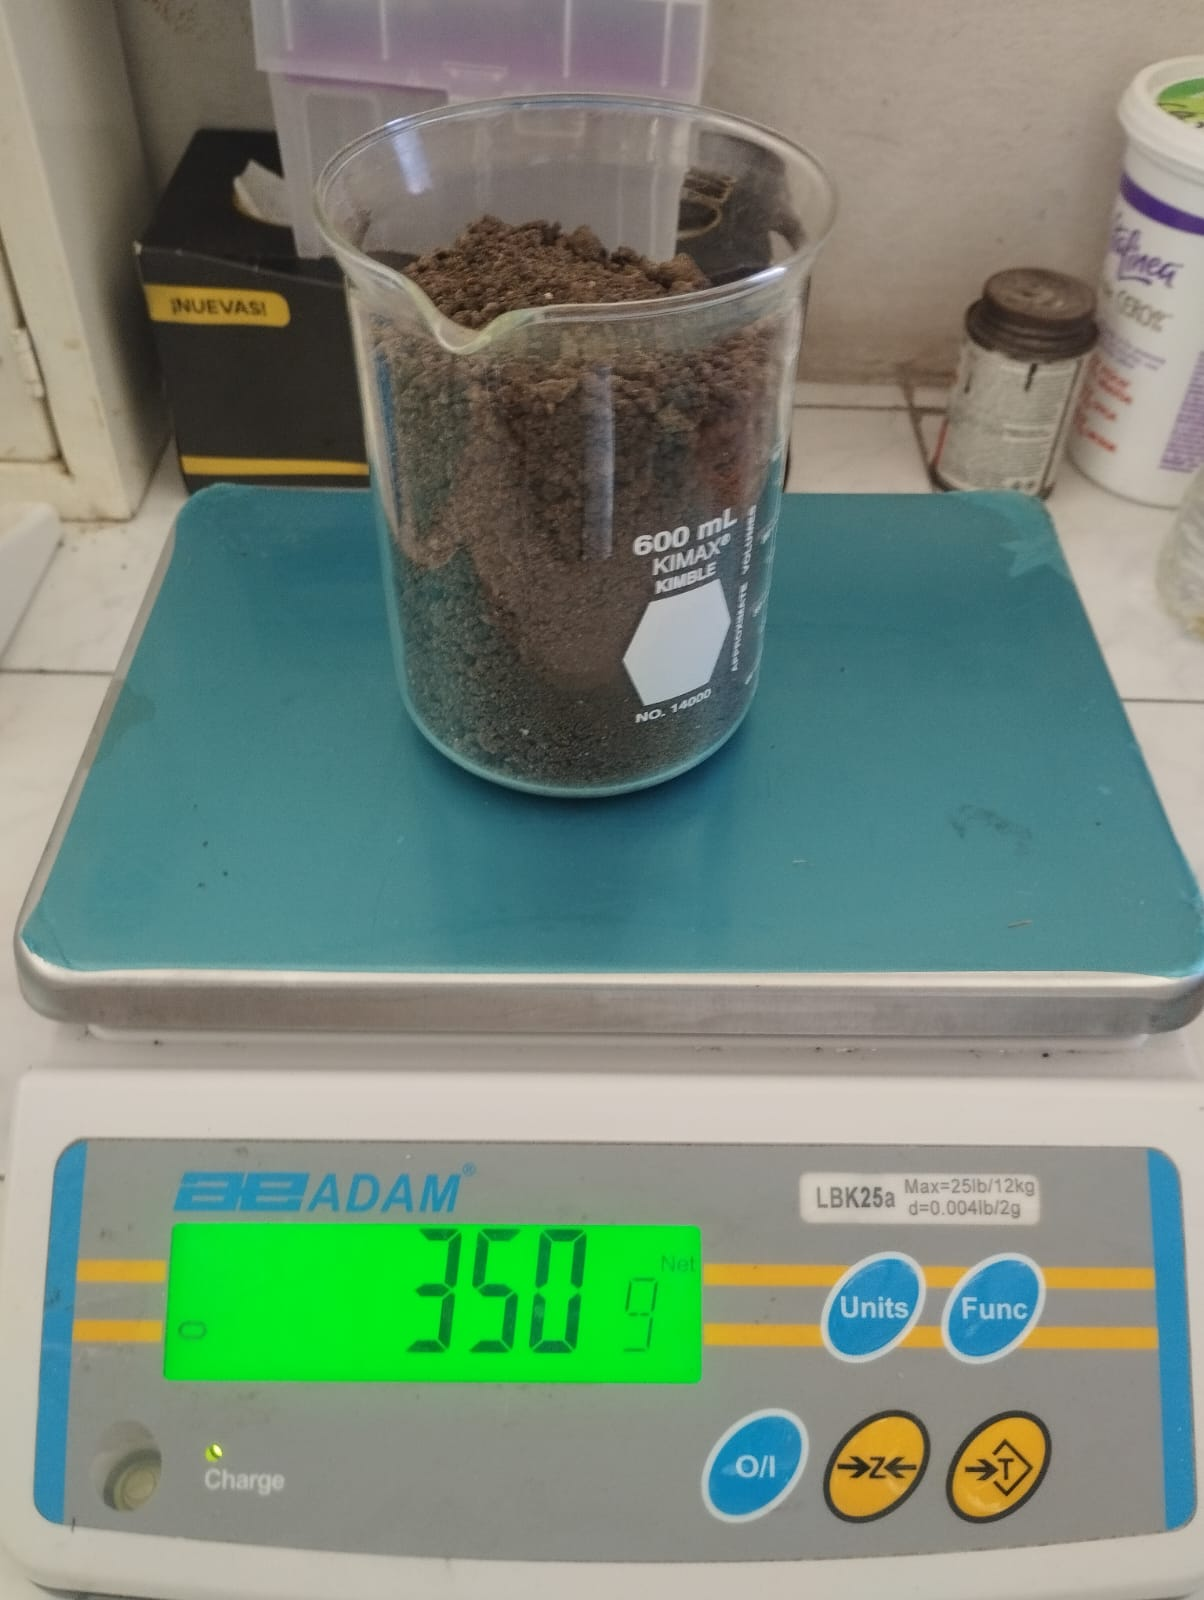
\includegraphics[width=3cm, height=5cm]{imagenes/humus}
				\caption{Se puede observar en la fotografía cuando se pesa el humus de lombriz con ayuda de una bascula.}
				\label{humus}
				\end{minipage}
			\end{figure}
			
			\textbf{3.}	Previo a su uso, el reactor se somete a un proceso de limpieza exhaustiva (Figura \ref{progra}), seguido de la aplicación estratégica de cinta de teflón en la zona roscada inferior para garantizar un sellado hermético. Finalmente, se procede al ensamblaje mediante el apriete controlado del tornillo, asegurando así la integridad del sistema.
			
			
			
			\textbf{4.}	Se carga el reactor con 6.0 L de agua desmineralizada, dosificados mediante un vaso de precipitado de 1 L calibrado. Posteriormente, se incorporan los 180 g de bagazo de caña previamente pesados y contenidos en la bolsa de 3 kg, siguiendo el procedimiento ilustrado en la Figura \ref{baciad}.
			

				\begin{figure}[H]
				\centering
				\begin{minipage}{0.46\textwidth}
					\centering
					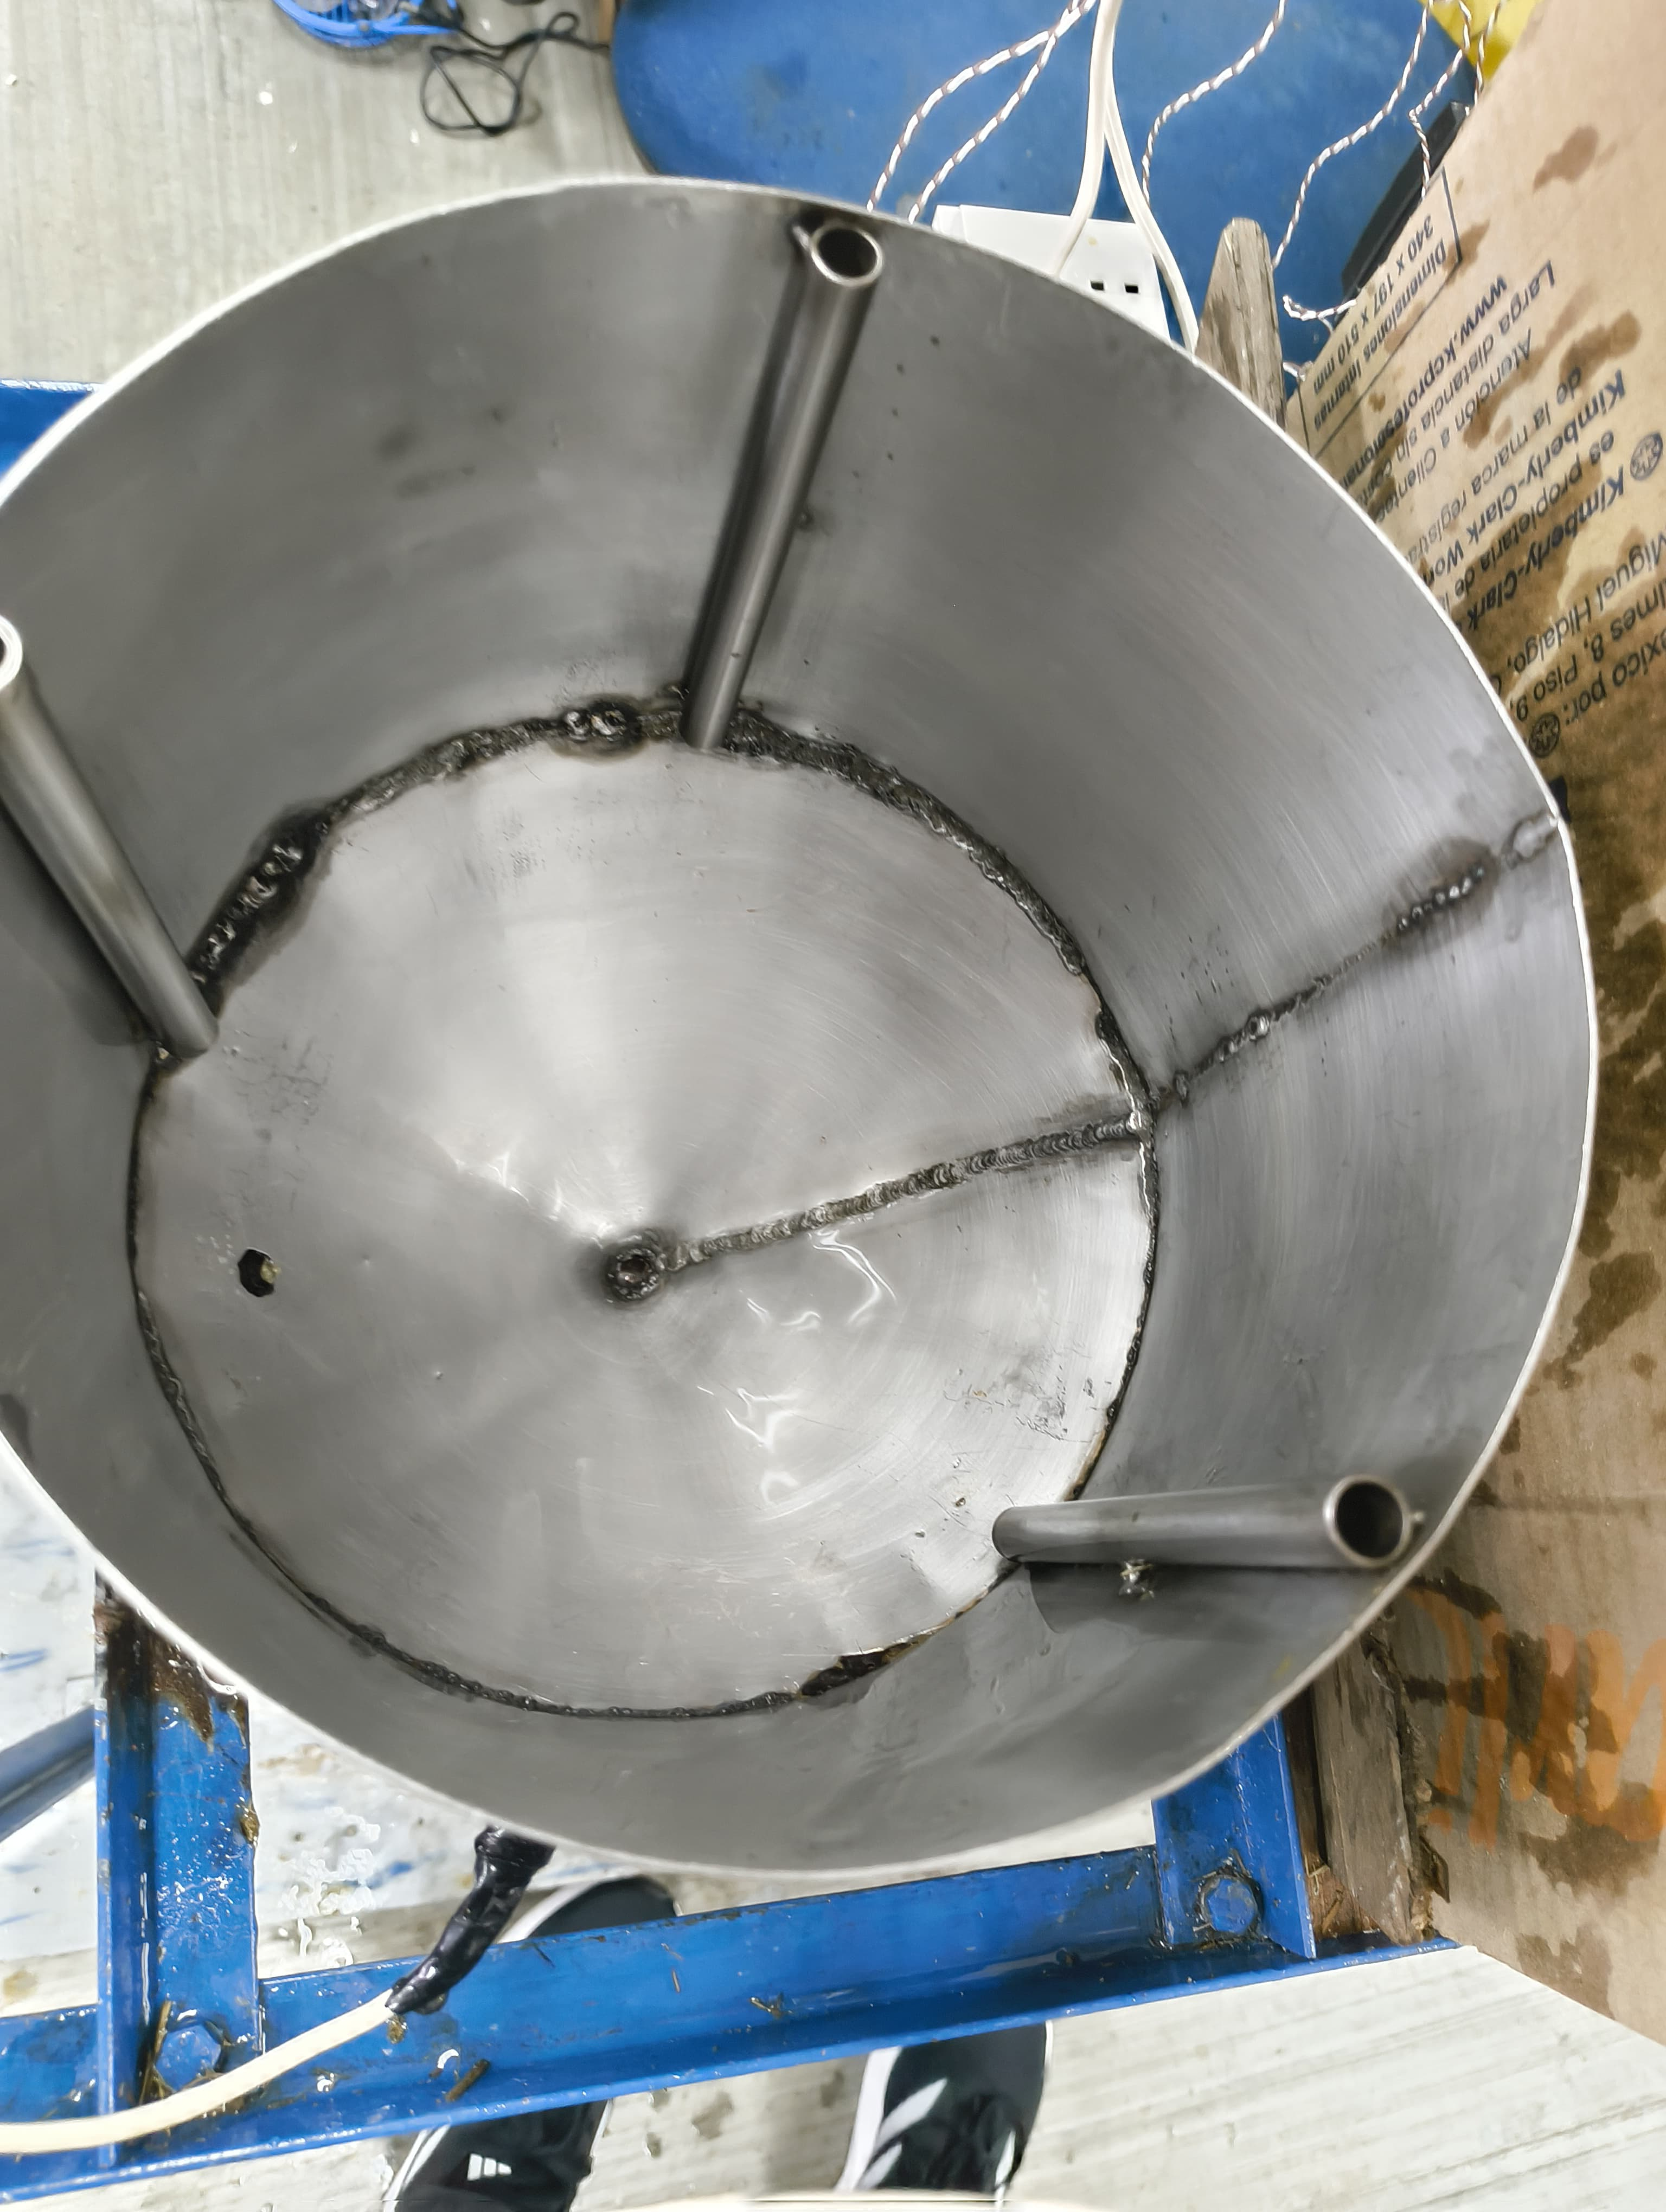
\includegraphics[width=4cm, height=5cm]{imagenes/reactor limpio} % Cambia "imagen1.jpg" por el nombre de tu archivo
					\caption{Fotografía muestra el reactor después de limpiarlo.}
					\label{progra}
				\end{minipage}
				\hfill
				\begin{minipage}{0.48\textwidth}
					\centering
					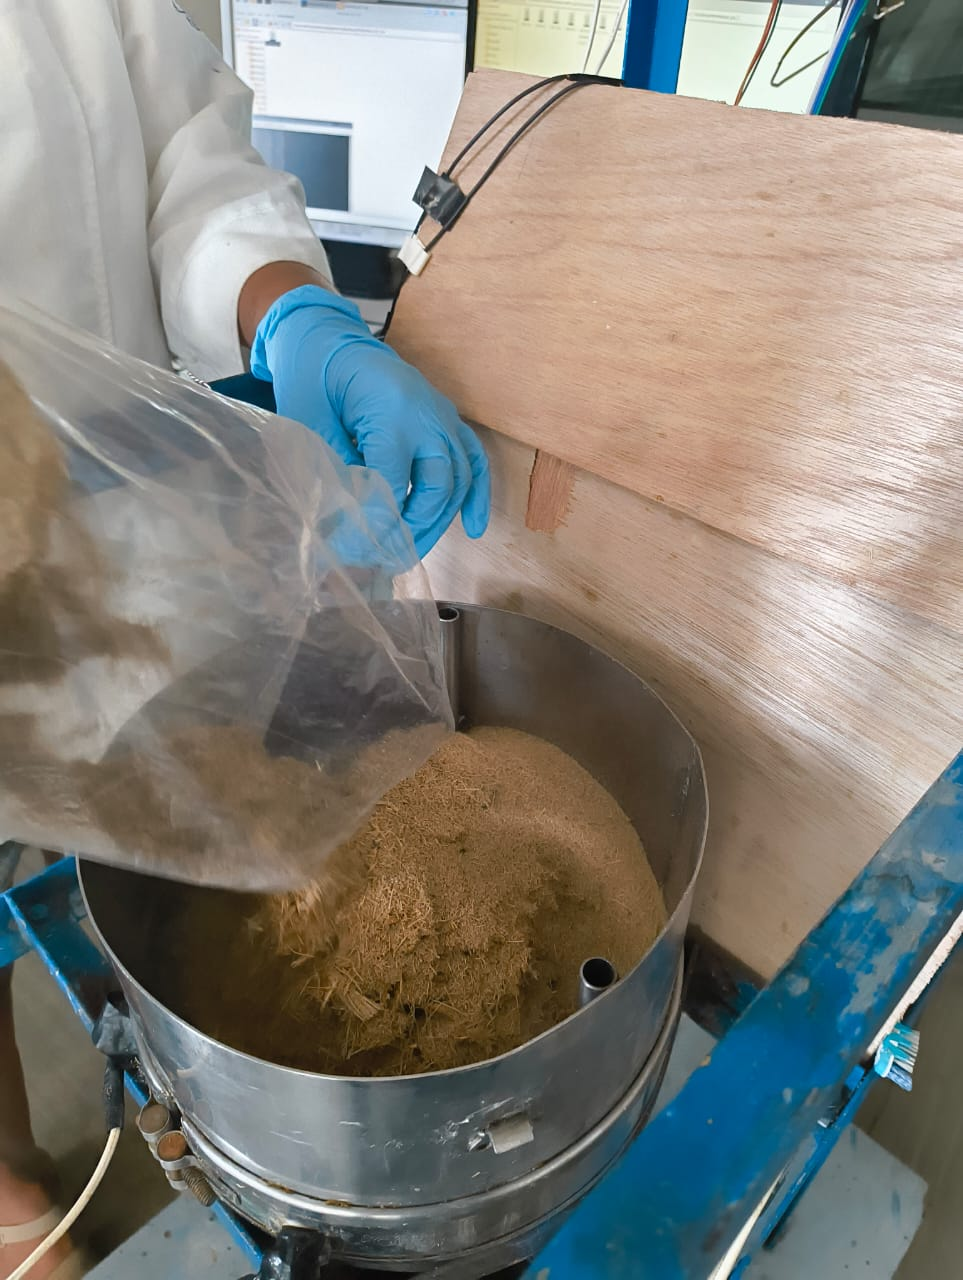
\includegraphics[width=4cm, height=5cm]{imagenes/biologico5} % Cambia "imagen2.jpg" por el nombre de tu archivo
					\caption{Se muestra como se agrega el bagazo de caña al reactor.}
					\label{baciad}
				\end{minipage}
			\end{figure}
			
			\textbf{5.}	Se adicionaron 300 g de humus de lombriz al reactor que ya contenía agua desmineralizada y bagazo de caña (Figura \ref{humus2}).
			

			\textbf{6.} Se procede a sellar el reactor utilizando una tapa que incorpora el motor. Se colocan los sensores de tipo termopar K en los tubos de un centímetro de diámetro, asegurándose de que estén correctamente posicionados. Para evitar la fuga de vapor, se utiliza algodón para sellar adecuadamente los tubos. Además, se emplean láminas de aluminio y cinta aislante o térmica para garantizar un cierre hermético tanto alrededor de la tapa como en la zona de los sensores, tal como se observa en la Figura \ref{cellado del reactor}.
			
		
			
	\begin{figure}[H]
		\centering
		\begin{minipage}{0.46\textwidth}
			\centering
			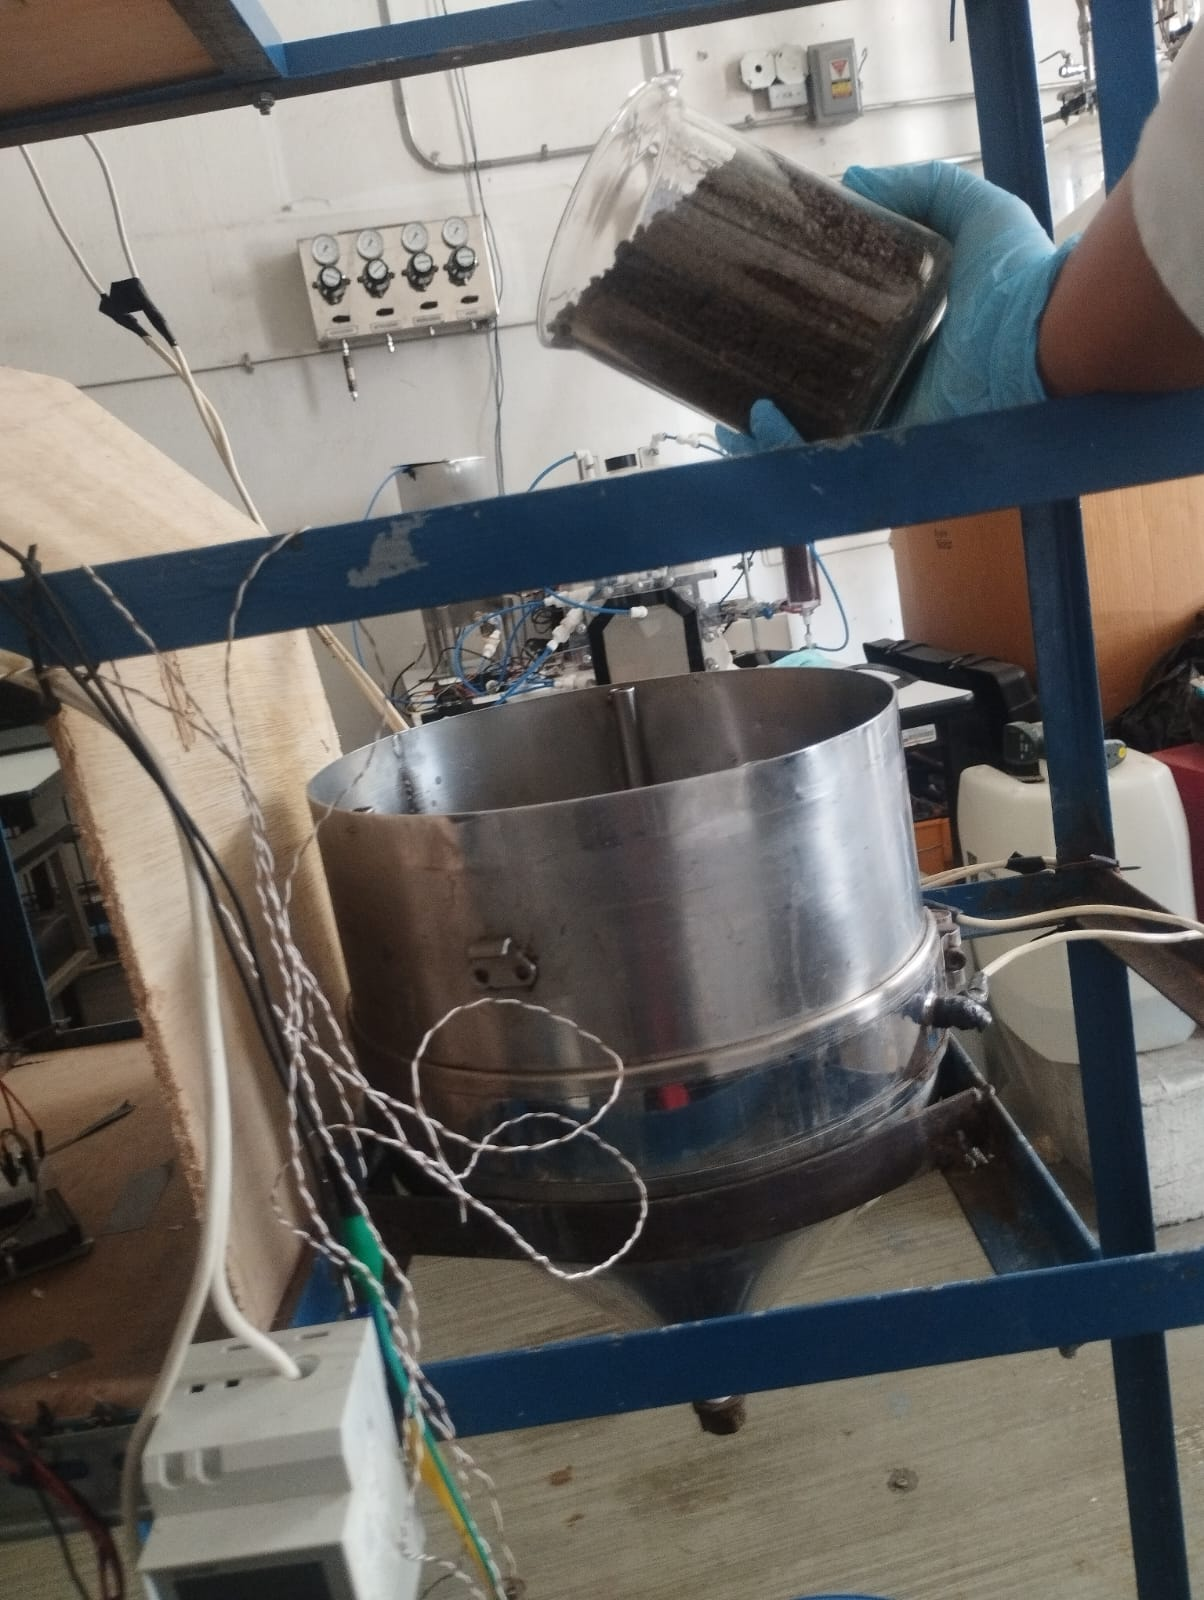
\includegraphics[width=3cm, height=5cm]{imagenes/humus2} % Cambia "imagen1.jpg" por el nombre de tu archivo
			\caption{Fotografía que muestra como se le agrega el humus de lombriz al reactor.}
				\label{humus2}
			\end{minipage}
			\hfill
			\begin{minipage}{0.48\textwidth}
				\centering
				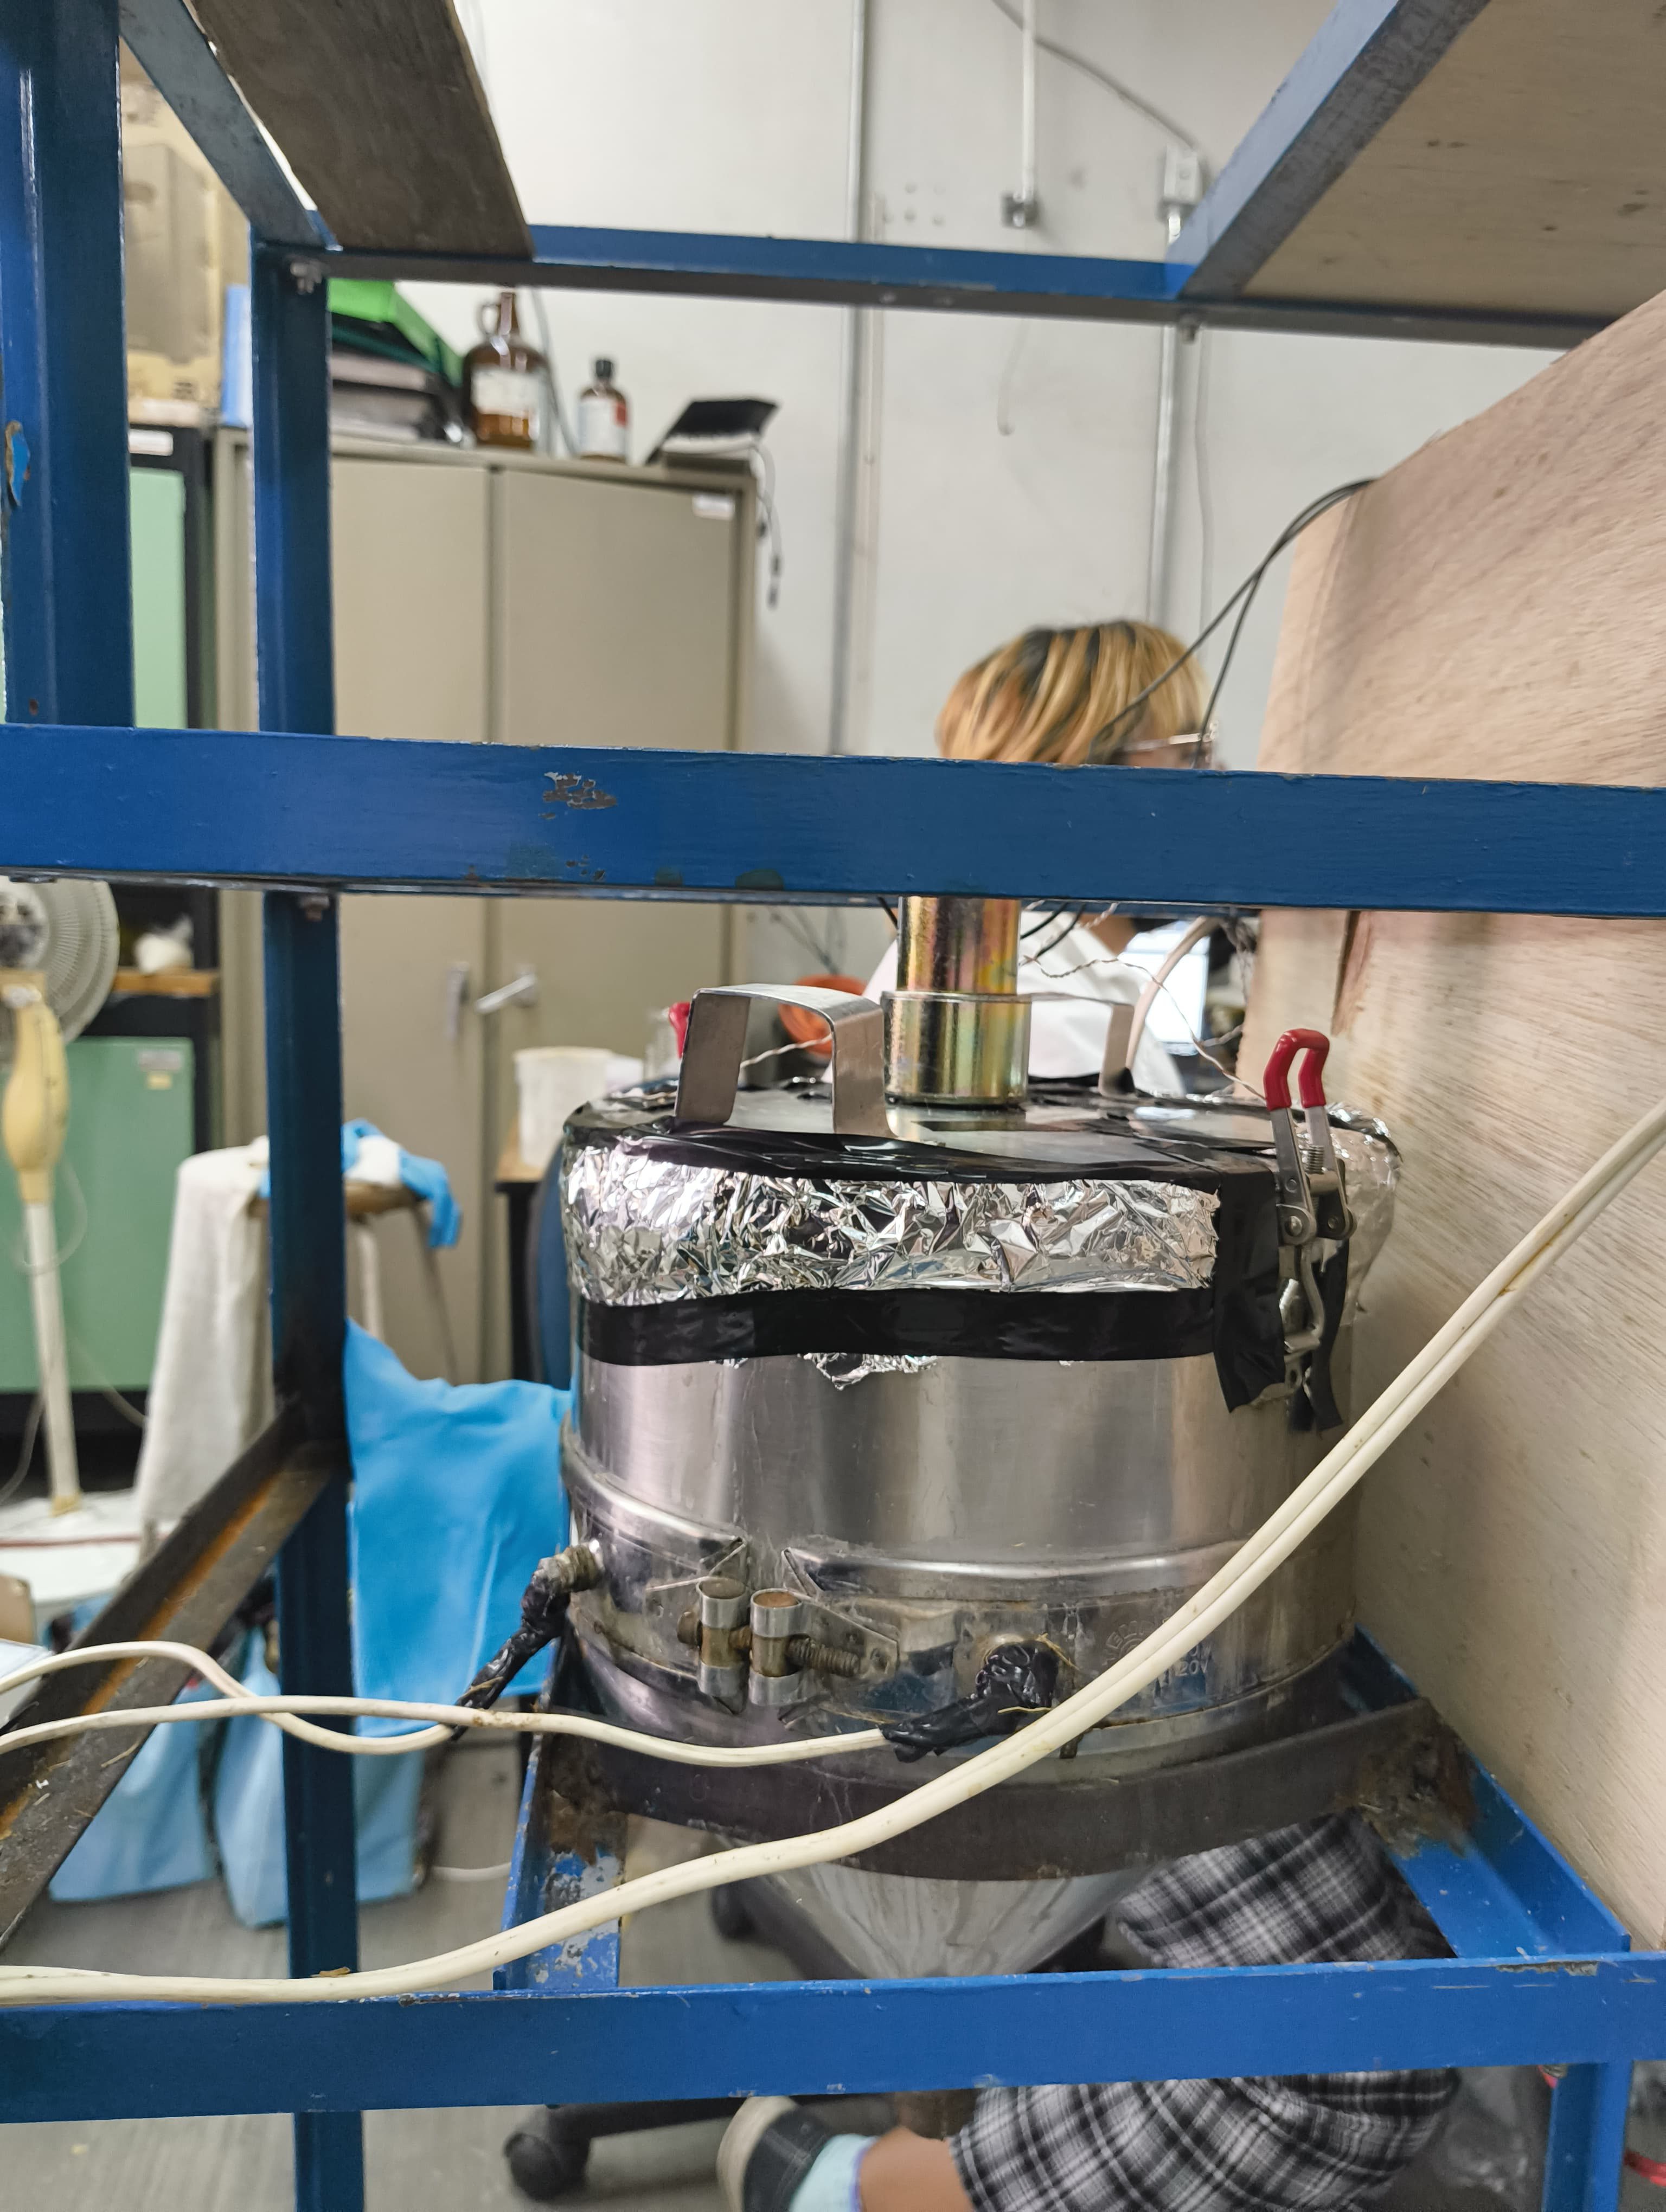
\includegraphics[width=3cm, height=5cm]{imagenes/cellado del reactor} % Cambia "imagen2.jpg" por el nombre de tu archivo
				\caption{Fotografía muestra el reactor después de sellarlo.}
				\label{cellado del reactor}
			\end{minipage}
		\end{figure}
		
			
			\textbf{7. } Se procede a conectar las Raspberry Pi y los monitores, así como las fuentes de alimentación y el sistema de respaldo (no-break). Se conectan los contactos múltiples necesarios, se configuran los dispositivos y se programa el control para mantener la temperatura conforme al diseño experimental descrito en el apartado \ref{DiseñopretratamientoBioogico}. El proceso se mantiene durante el tiempo estipulado para el pretratamiento, el diseño del control del control de temperatura, ver anexo \ref{diseño del control de temp}. Las Figuras \ref{progra 1} y \ref{progra 2} muestran las pantallas con el control en funcionamiento.
			
			\begin{figure}[H]
				\centering
				\begin{minipage}{0.46\textwidth}
					\centering
					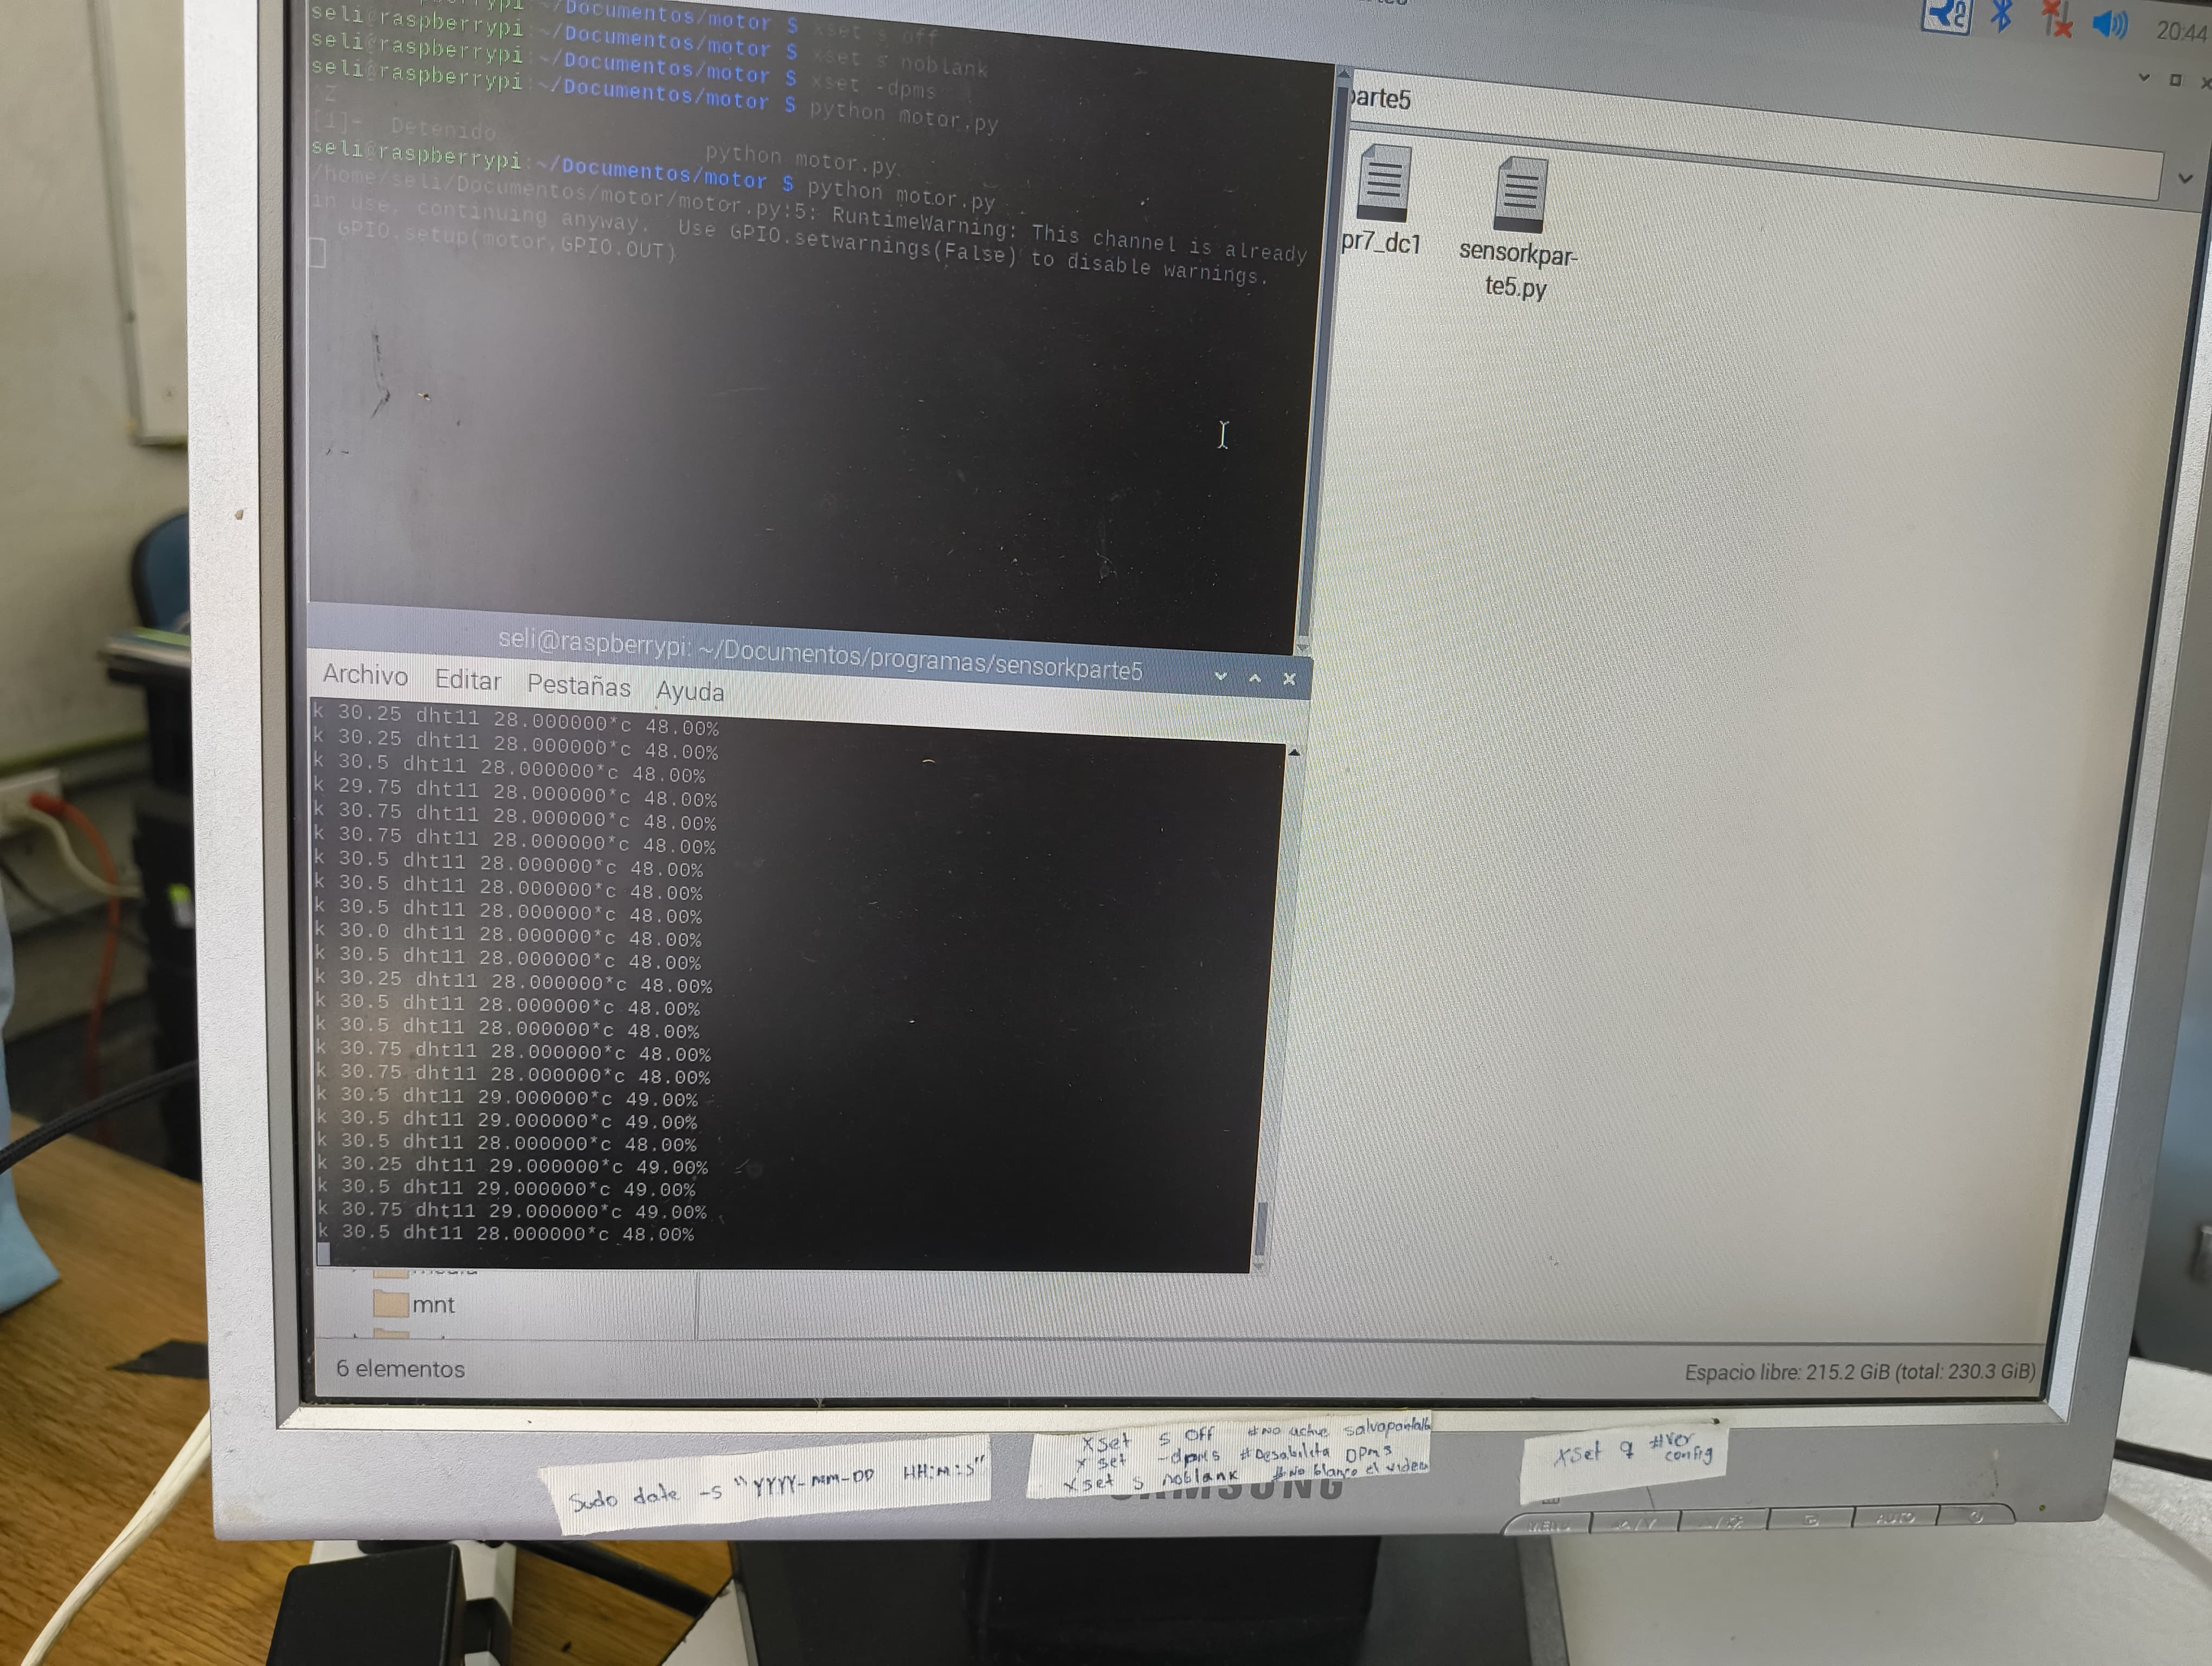
\includegraphics[width=5cm, height=3cm]{imagenes/programa1} % Cambia "imagen1.jpg" por el nombre de tu archivo
					\caption{Programa de la temperatura ambiente en marcha.}
					\label{progra 1}
				\end{minipage}
				\hfill
				\begin{minipage}{0.48\textwidth}
					\centering
					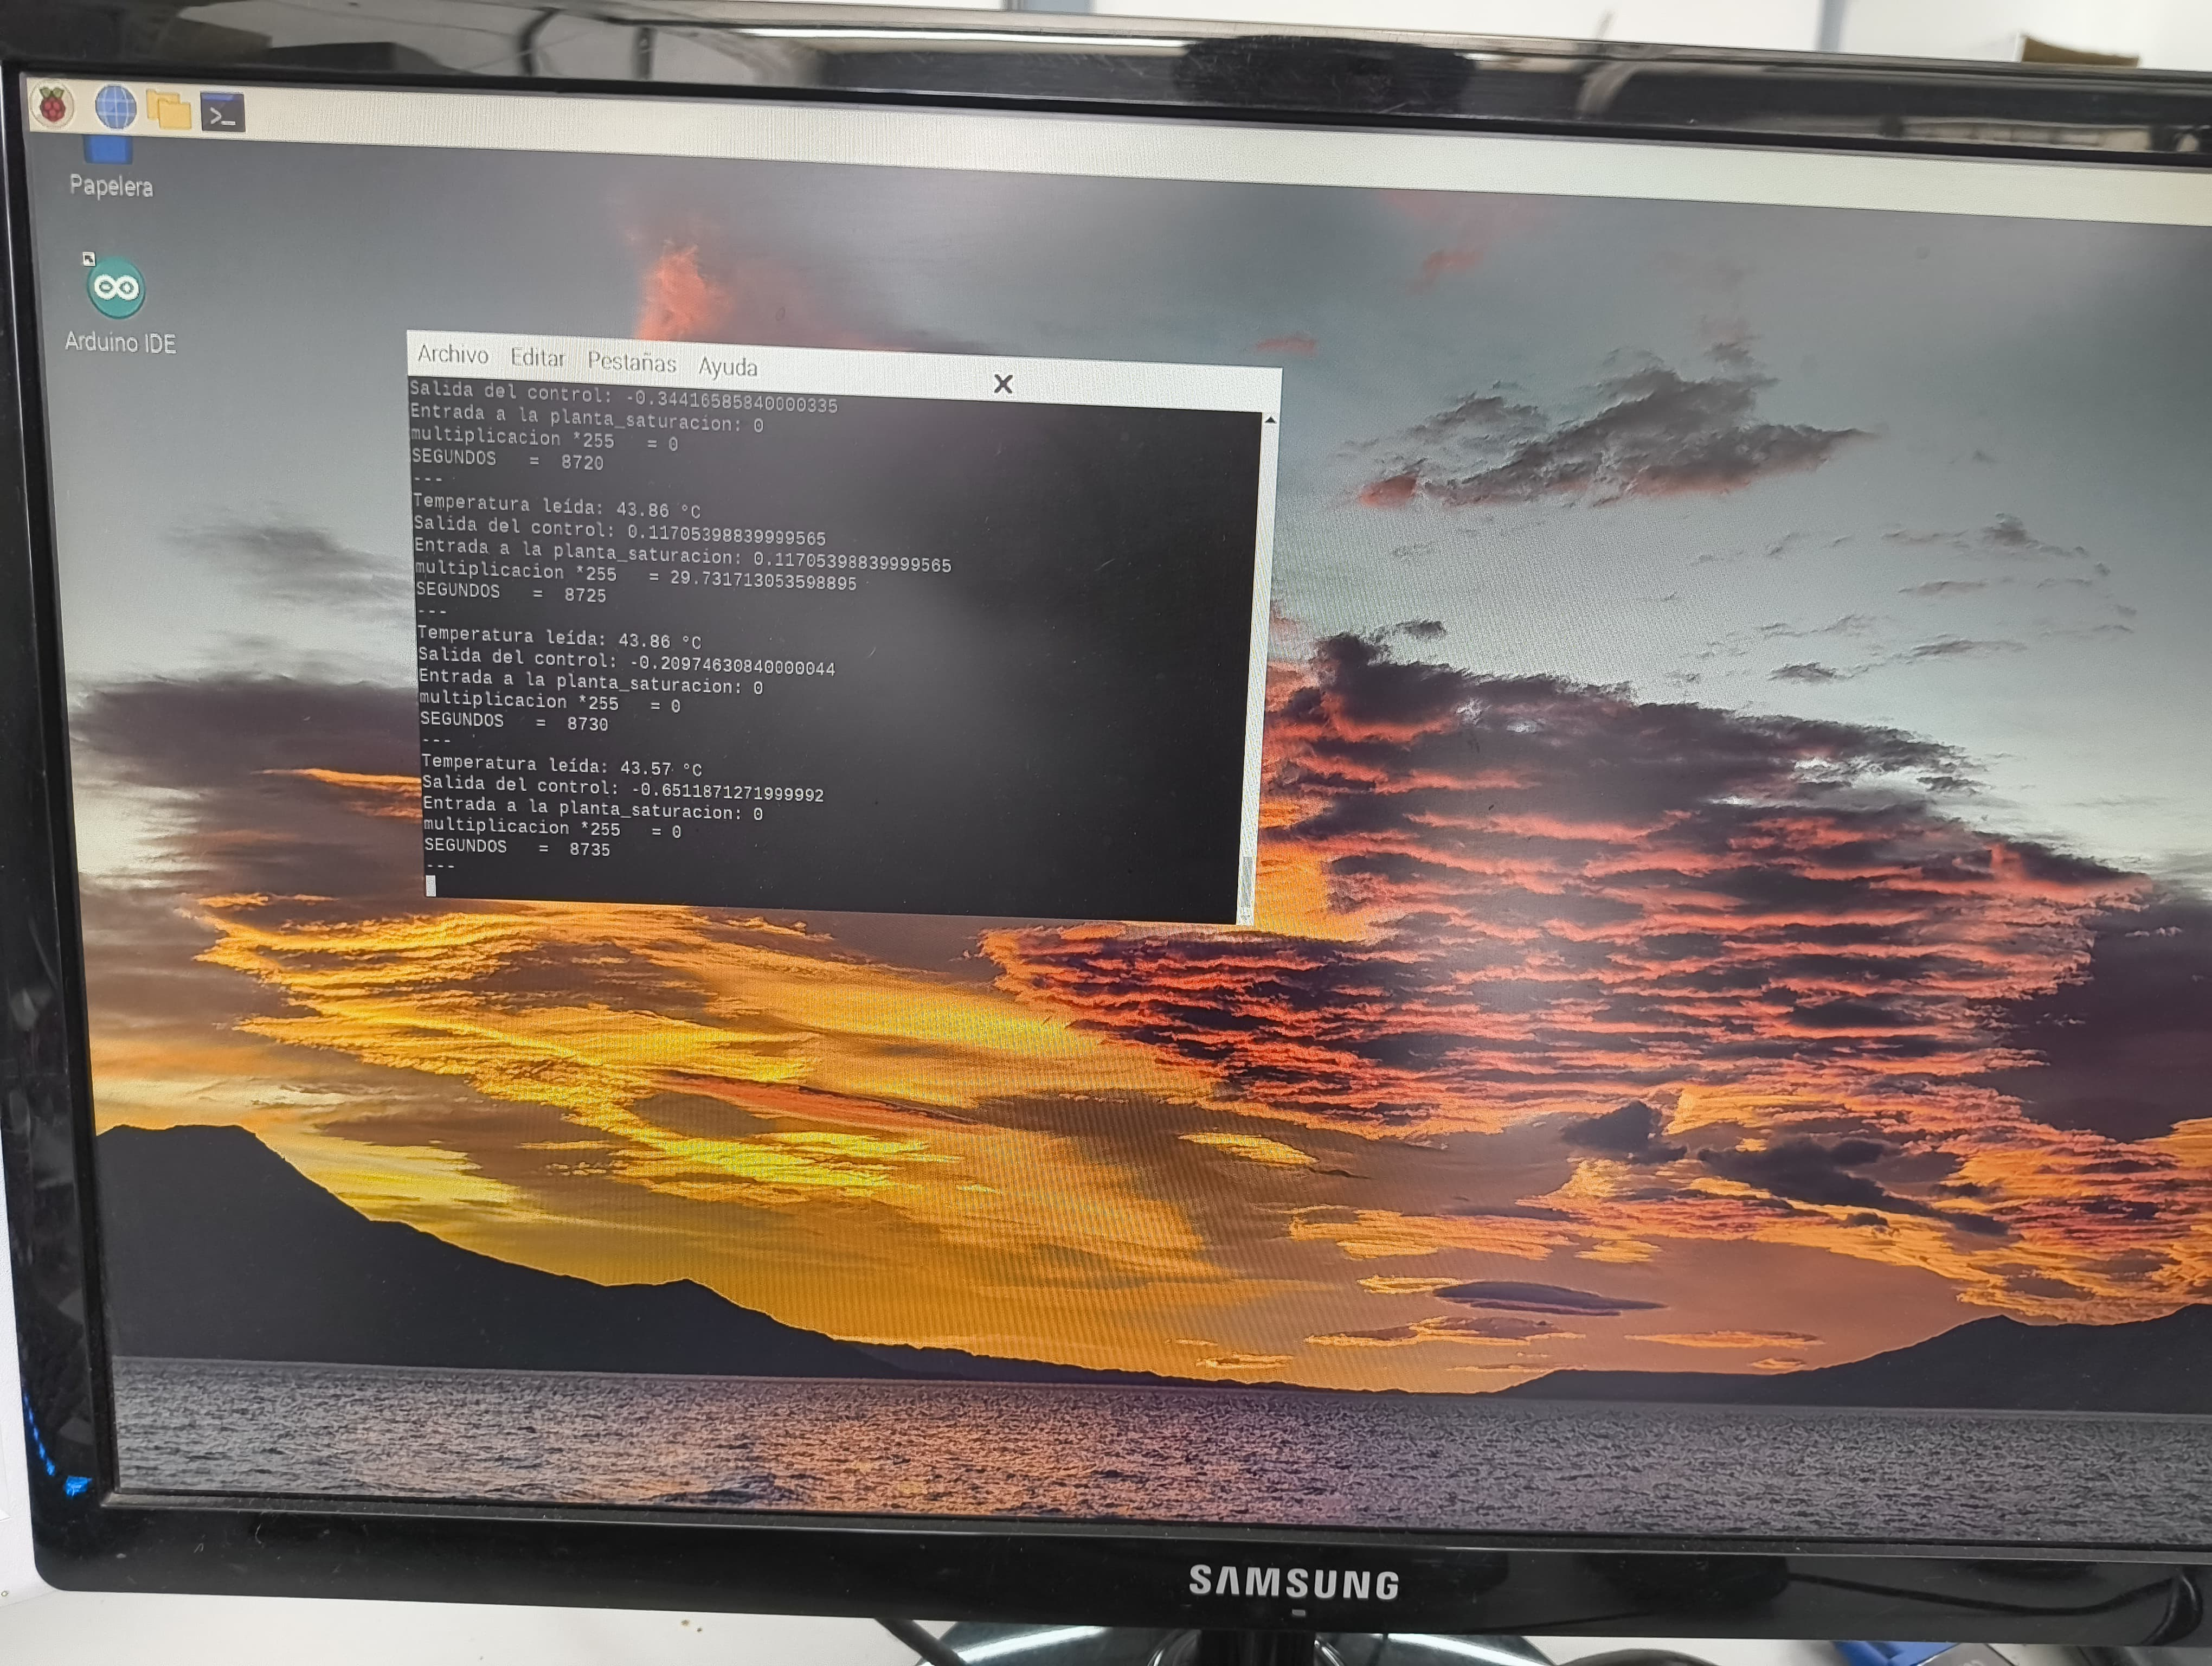
\includegraphics[width=5cm, height=3cm]{imagenes/programa2} % Cambia "imagen2.jpg" por el nombre de tu archivo
					\caption{Programa del control en marcha.}
					\label{progra 2}
				\end{minipage}
			\end{figure}
			

			
			%%%%%%%%%%%%%%%%%%%%%%%%%%%%%%%%%%%%%%%%%%%%%%%%%%%%%%%%%%%%%%%%%%%%%%%%%%%%%%%%%%%%%%%%%%%%%%%%%%%%%%%%%%%%%%%%%%%%%%%%%%%%%%%%%%%%%%%%%
			
			\subsubsection{Pretratamiento Alcalino}
			El pretratamiento alcalino es un tipo de pretratamiento, a continuación se muestran los pasos y los insumos para llevar a cabo las pruebas experimentales.		
			\\[1 em]
			\textbf{Compuestos} 
			\\[0.5em]
			
			\begin{tabular}{p{0.3\textwidth}p{0.3\textwidth}}
				\textcolor{blue}{$\bullet$} \textit{Hidróxido de sodio} &	\textcolor{blue}{$\bullet$}\textit{ Bagazo de caña} 
			\end{tabular} \\[ 1em]
			
			
			
			\textbf{Materiales} 
			\\[1 em]
			
			\begin{tabular}{p{0.3\textwidth}p{0.3\textwidth}p{0.3\textwidth}}
				$\bullet$ \textit{Agua desmineralizada }& $\bullet$ \textit{Algodón }& $\bullet$ \textit{Bolsa plástica de 30×40 cm} \\
				$\bullet$ \textit{Báscula} & $\bullet$ \textit{Cinta aislante} & $\bullet$ \textit{Cinta de teflón}
			\end{tabular}
			\\[0.5em]
			
			
			\textbf{Procedimiento}
			\\[0.5em]
			
			\textbf{1.}	La cantidad de bagazo se determina mediante pesaje con báscula (precisión ±0.2 g) usando una bolsa plástica de 30×40 cm como contenedor, hasta alcanzar 180 g. Alternativamente, cuando se emplea la medida de 1 cm, se utiliza directamente el material preclasificado y calibrado, según se ilustra en la Figura \ref{bagazo1}.\\
			
			\textbf{2.} Mediante una báscula analítica (precisión ±0.2 g) y vaso de precipitado de vidrio, se pesan exactamente 120 g de hidróxido de sodio en pellets, asegurando la exactitud requerida para el proceso.Ver Figura \ref{cernir_bagazo_hidroxidopesado}.
			
			
			\begin{figure}[H]
				\centering
				\begin{minipage}{0.46\textwidth}
					\centering
					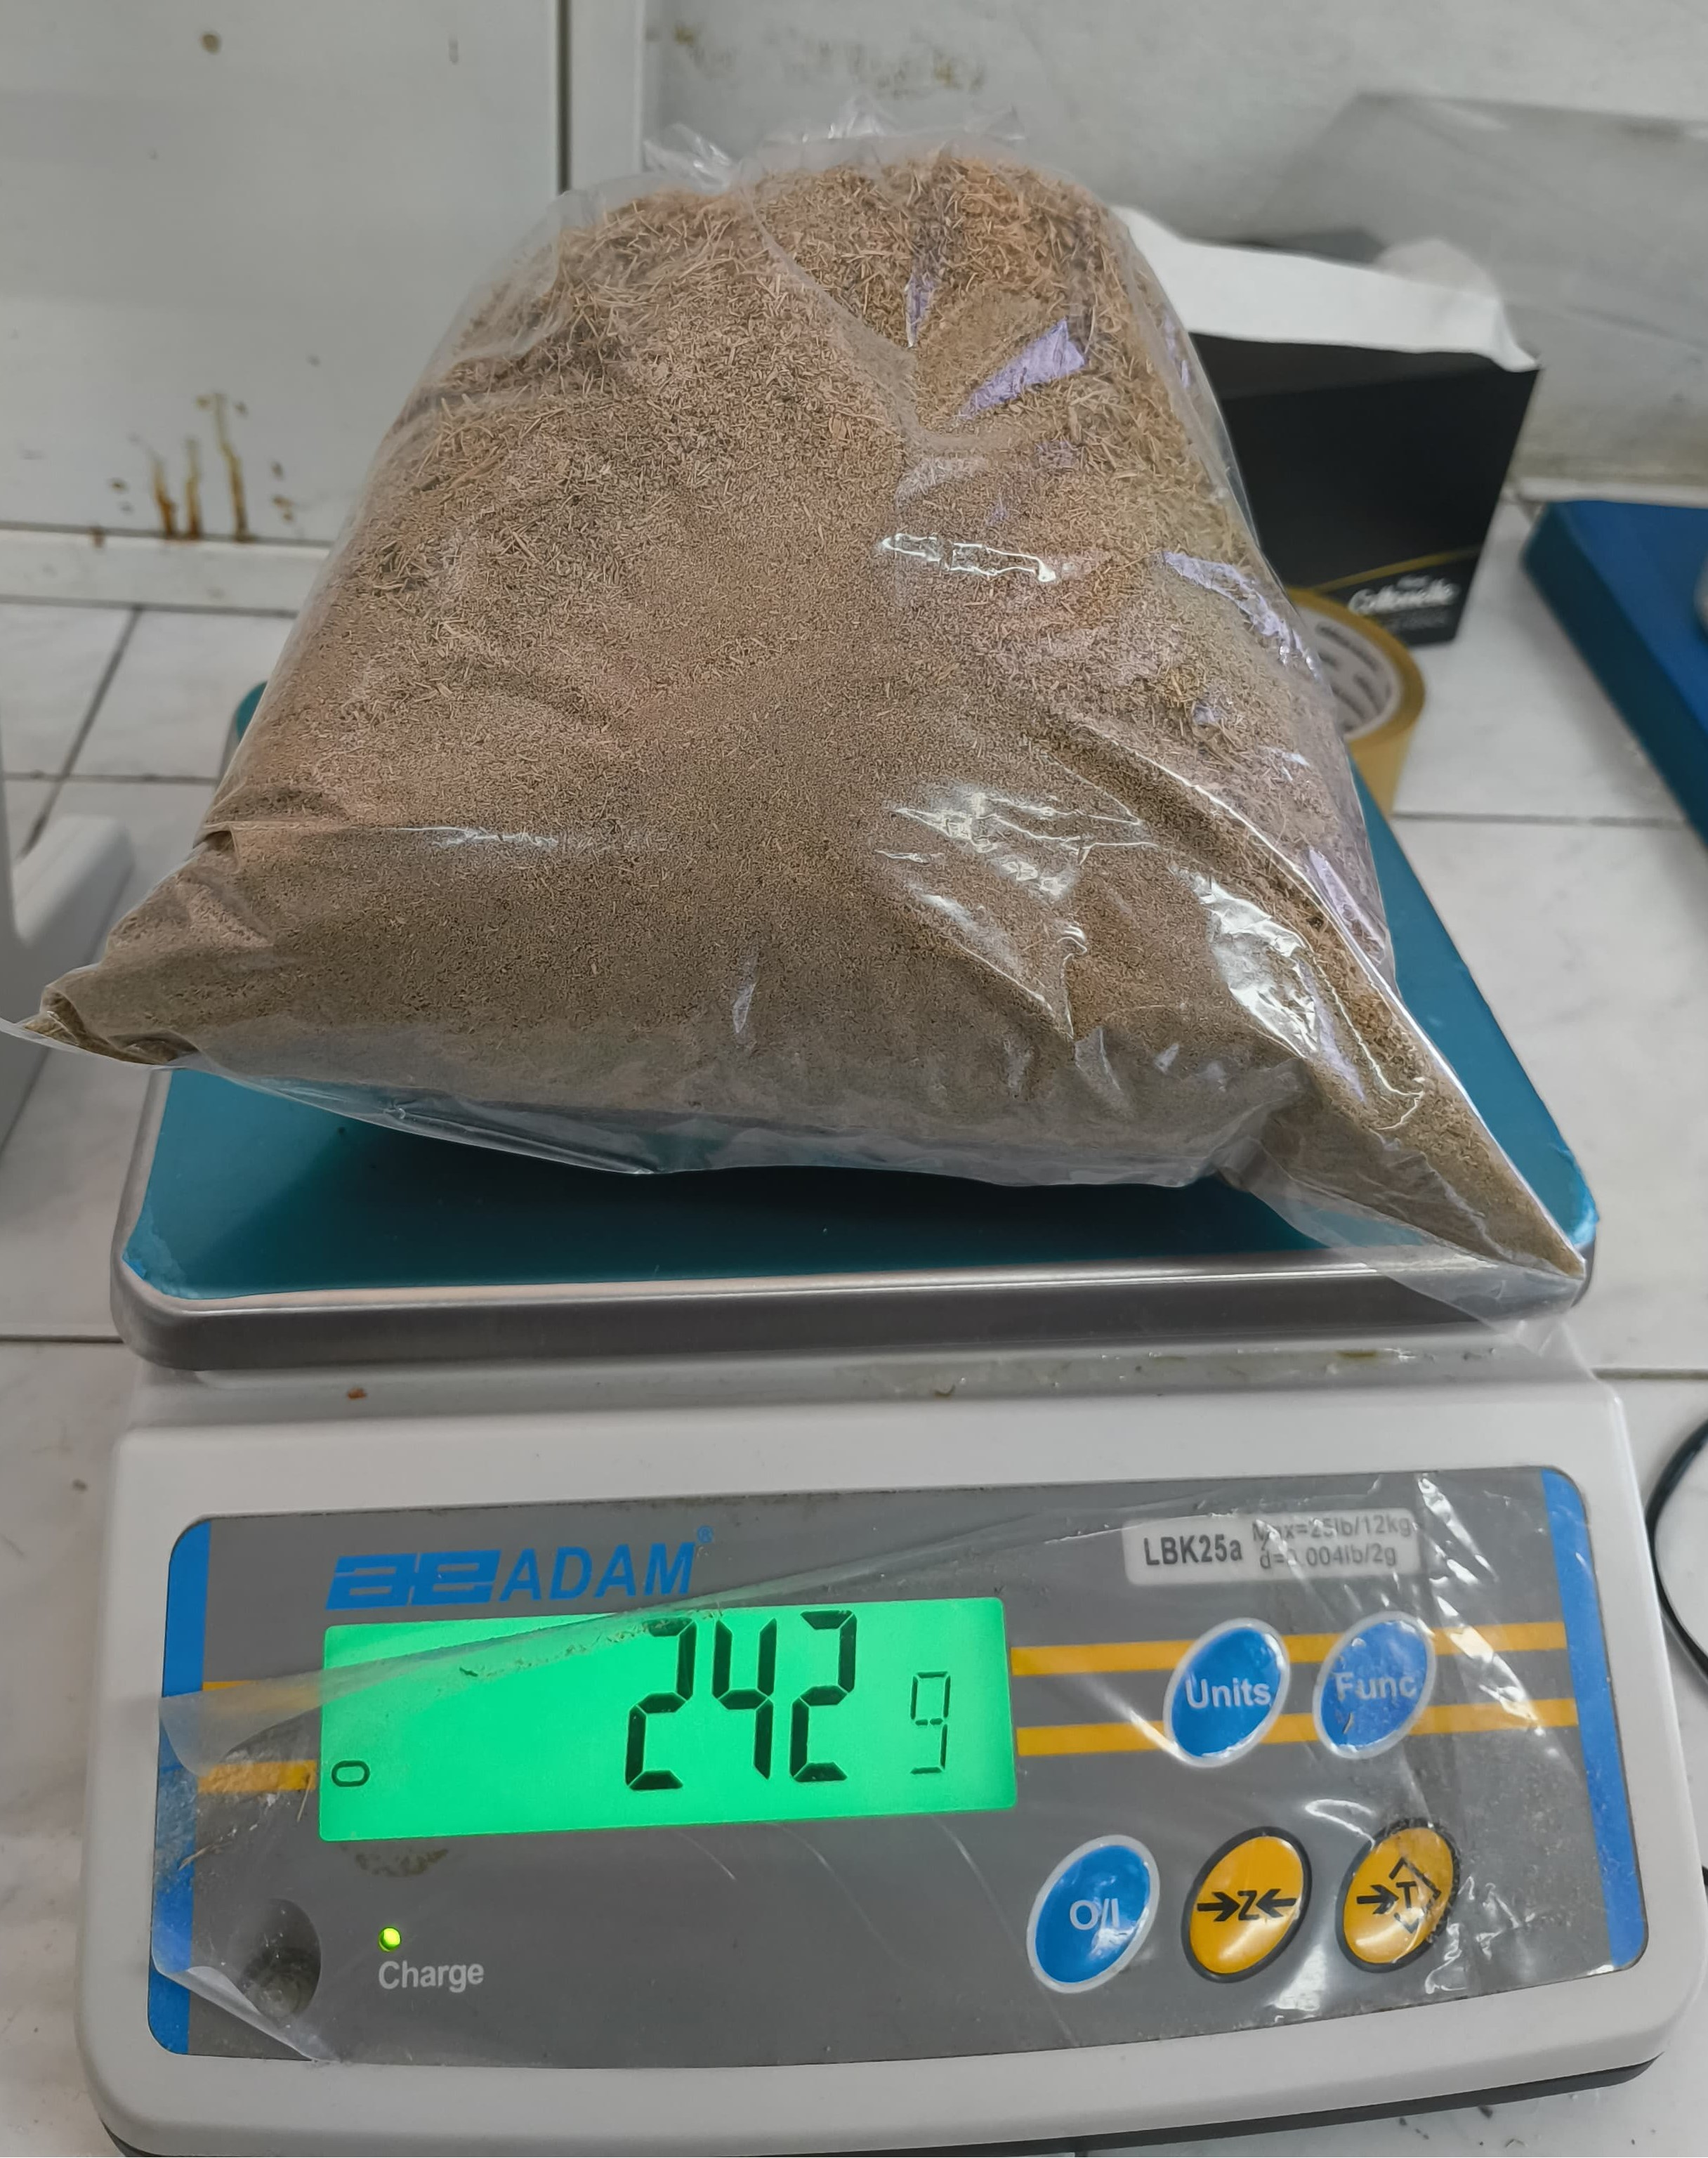
\includegraphics[width=3cm, height=5cm]{imagenes/pesado4}
					\caption{Bagazo de 1 cm.}
					\label{bagazo1}
				\end{minipage}
				\hfill
				\begin{minipage}{0.48\textwidth}
					\centering
					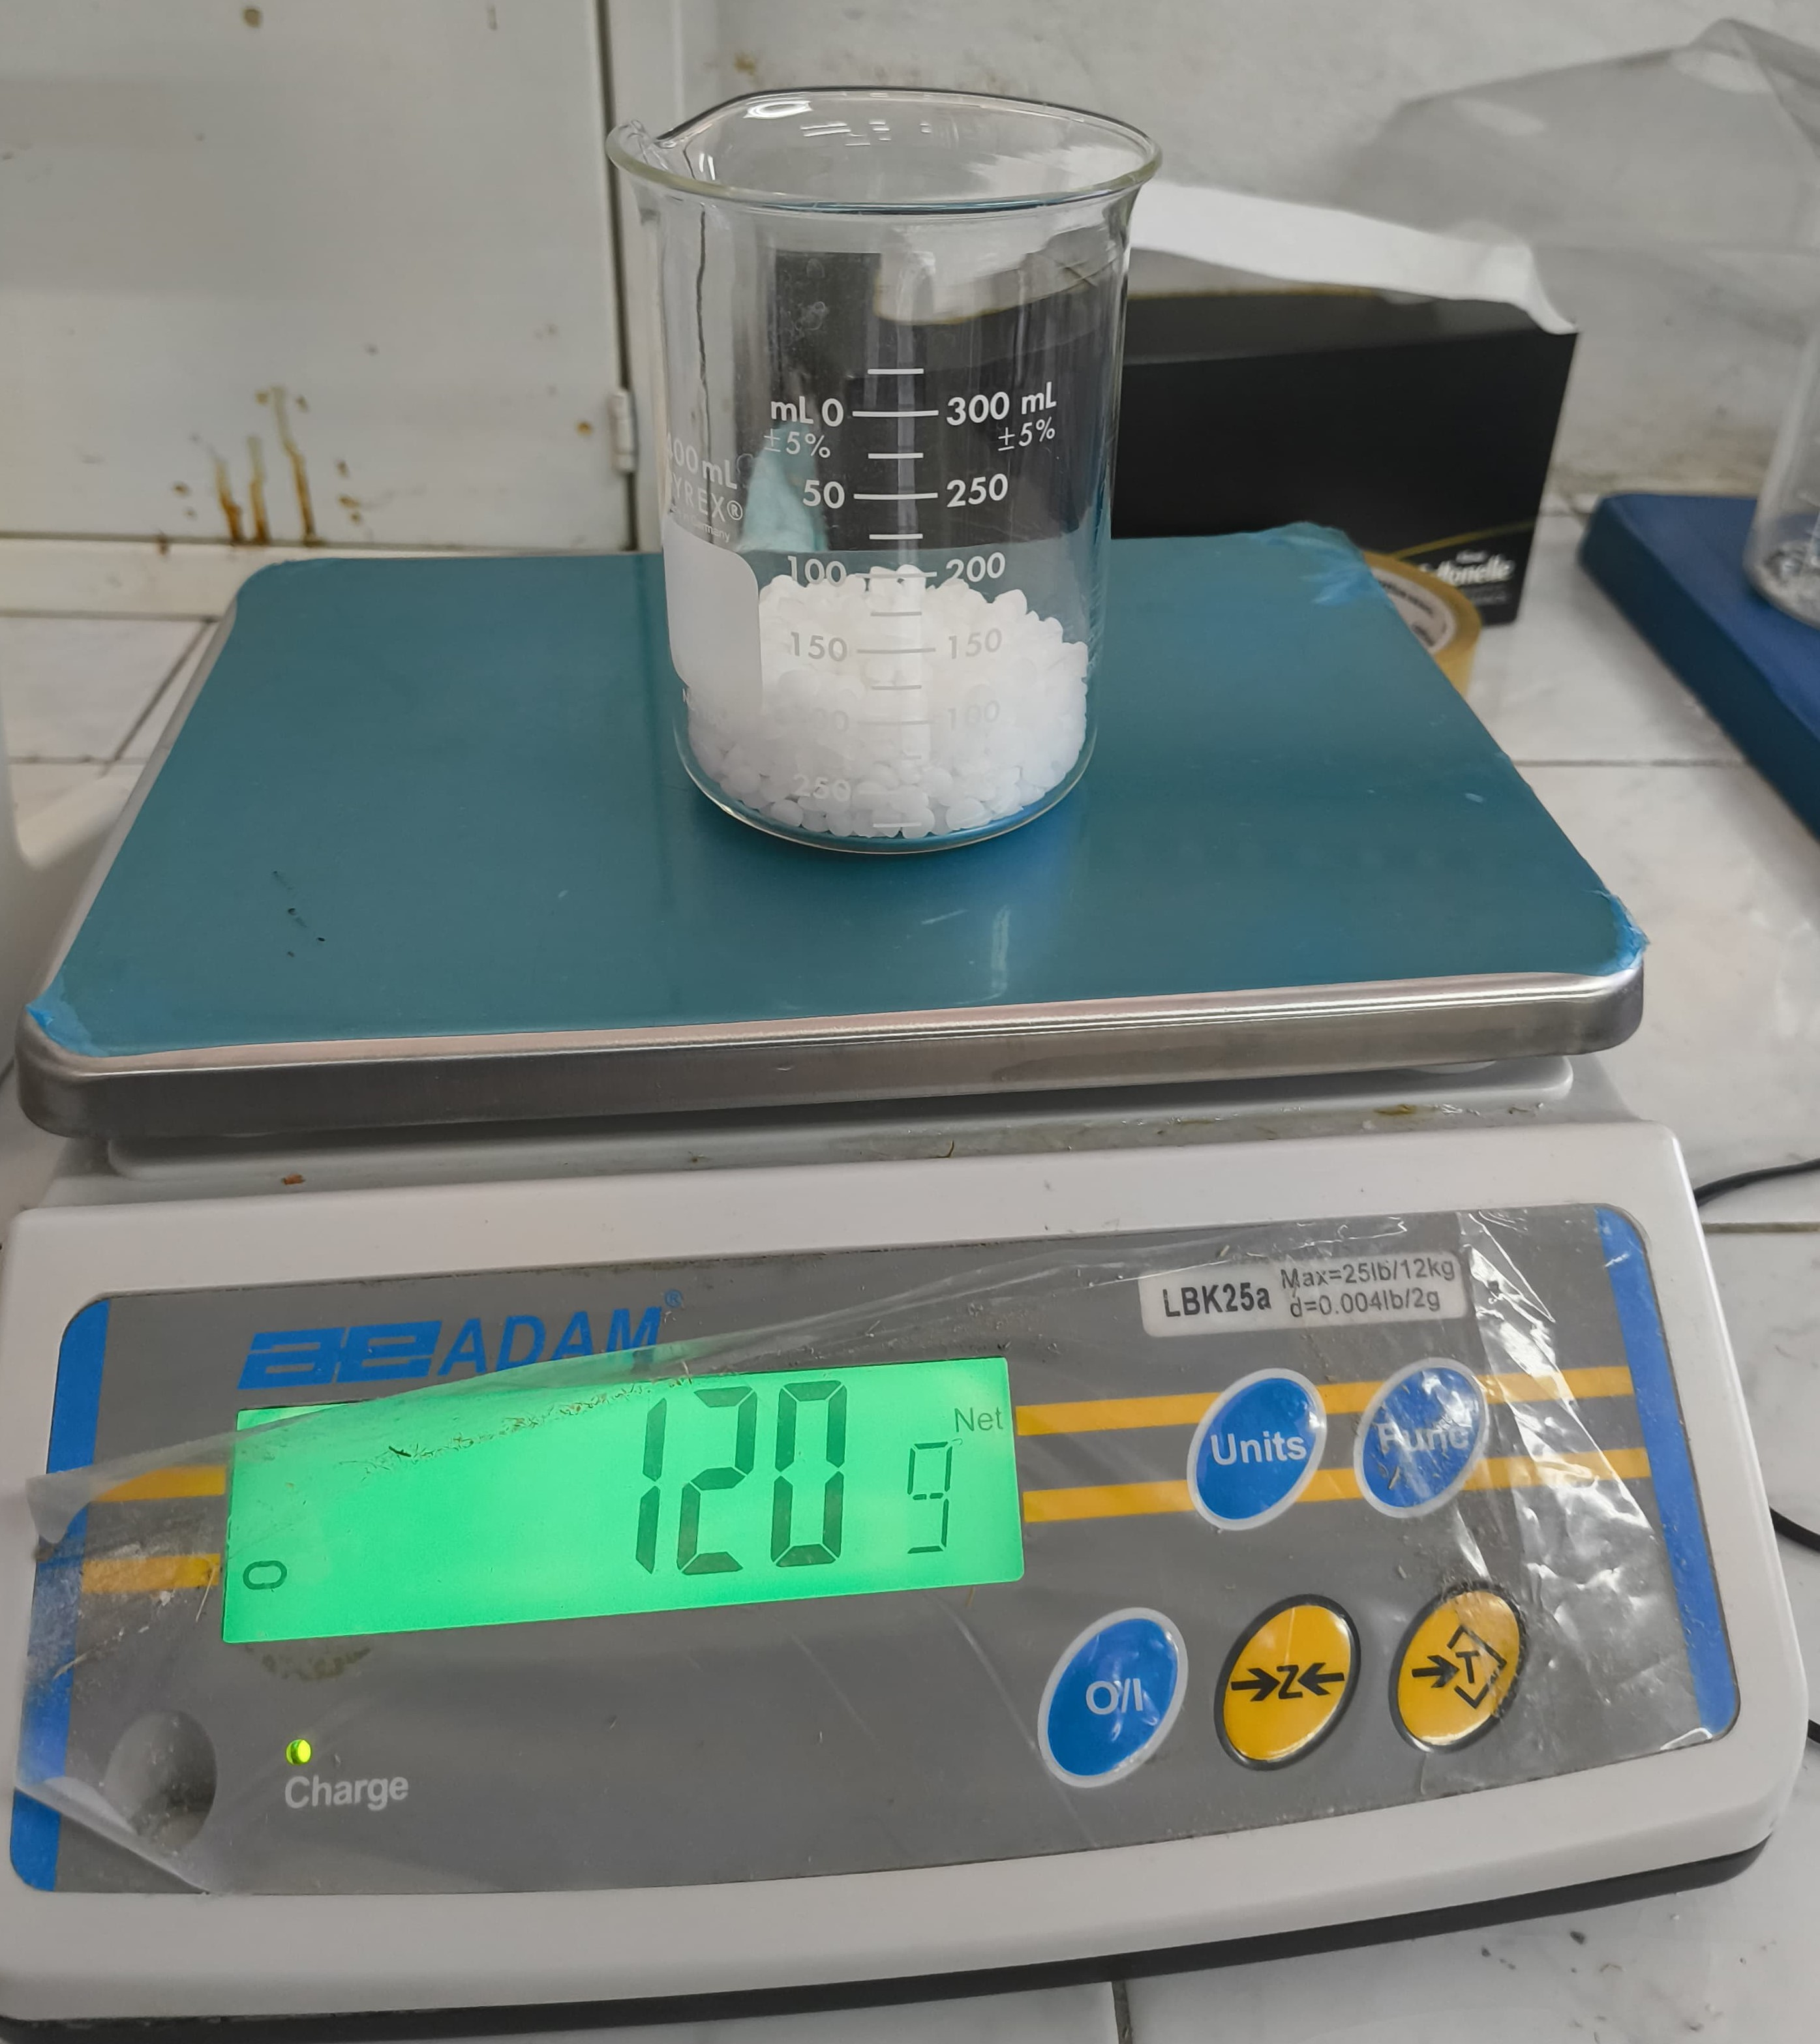
\includegraphics[width=3cm, height=5cm]{imagenes/hidroxido_pesado}
					\caption{El hidroxido es pesado en una bascula.}
					\label{cernir_bagazo_hidroxidopesado}
				\end{minipage}
			\end{figure}
			
			
			
			\textbf{3.} El reactor y su mezclador se enjuagan minuciosamente con agua desmineralizada para garantizar su limpieza óptima antes de su uso, eliminando cualquier residuo que pueda afectar el proceso.
			\begin{figure} [H]
				\centering
				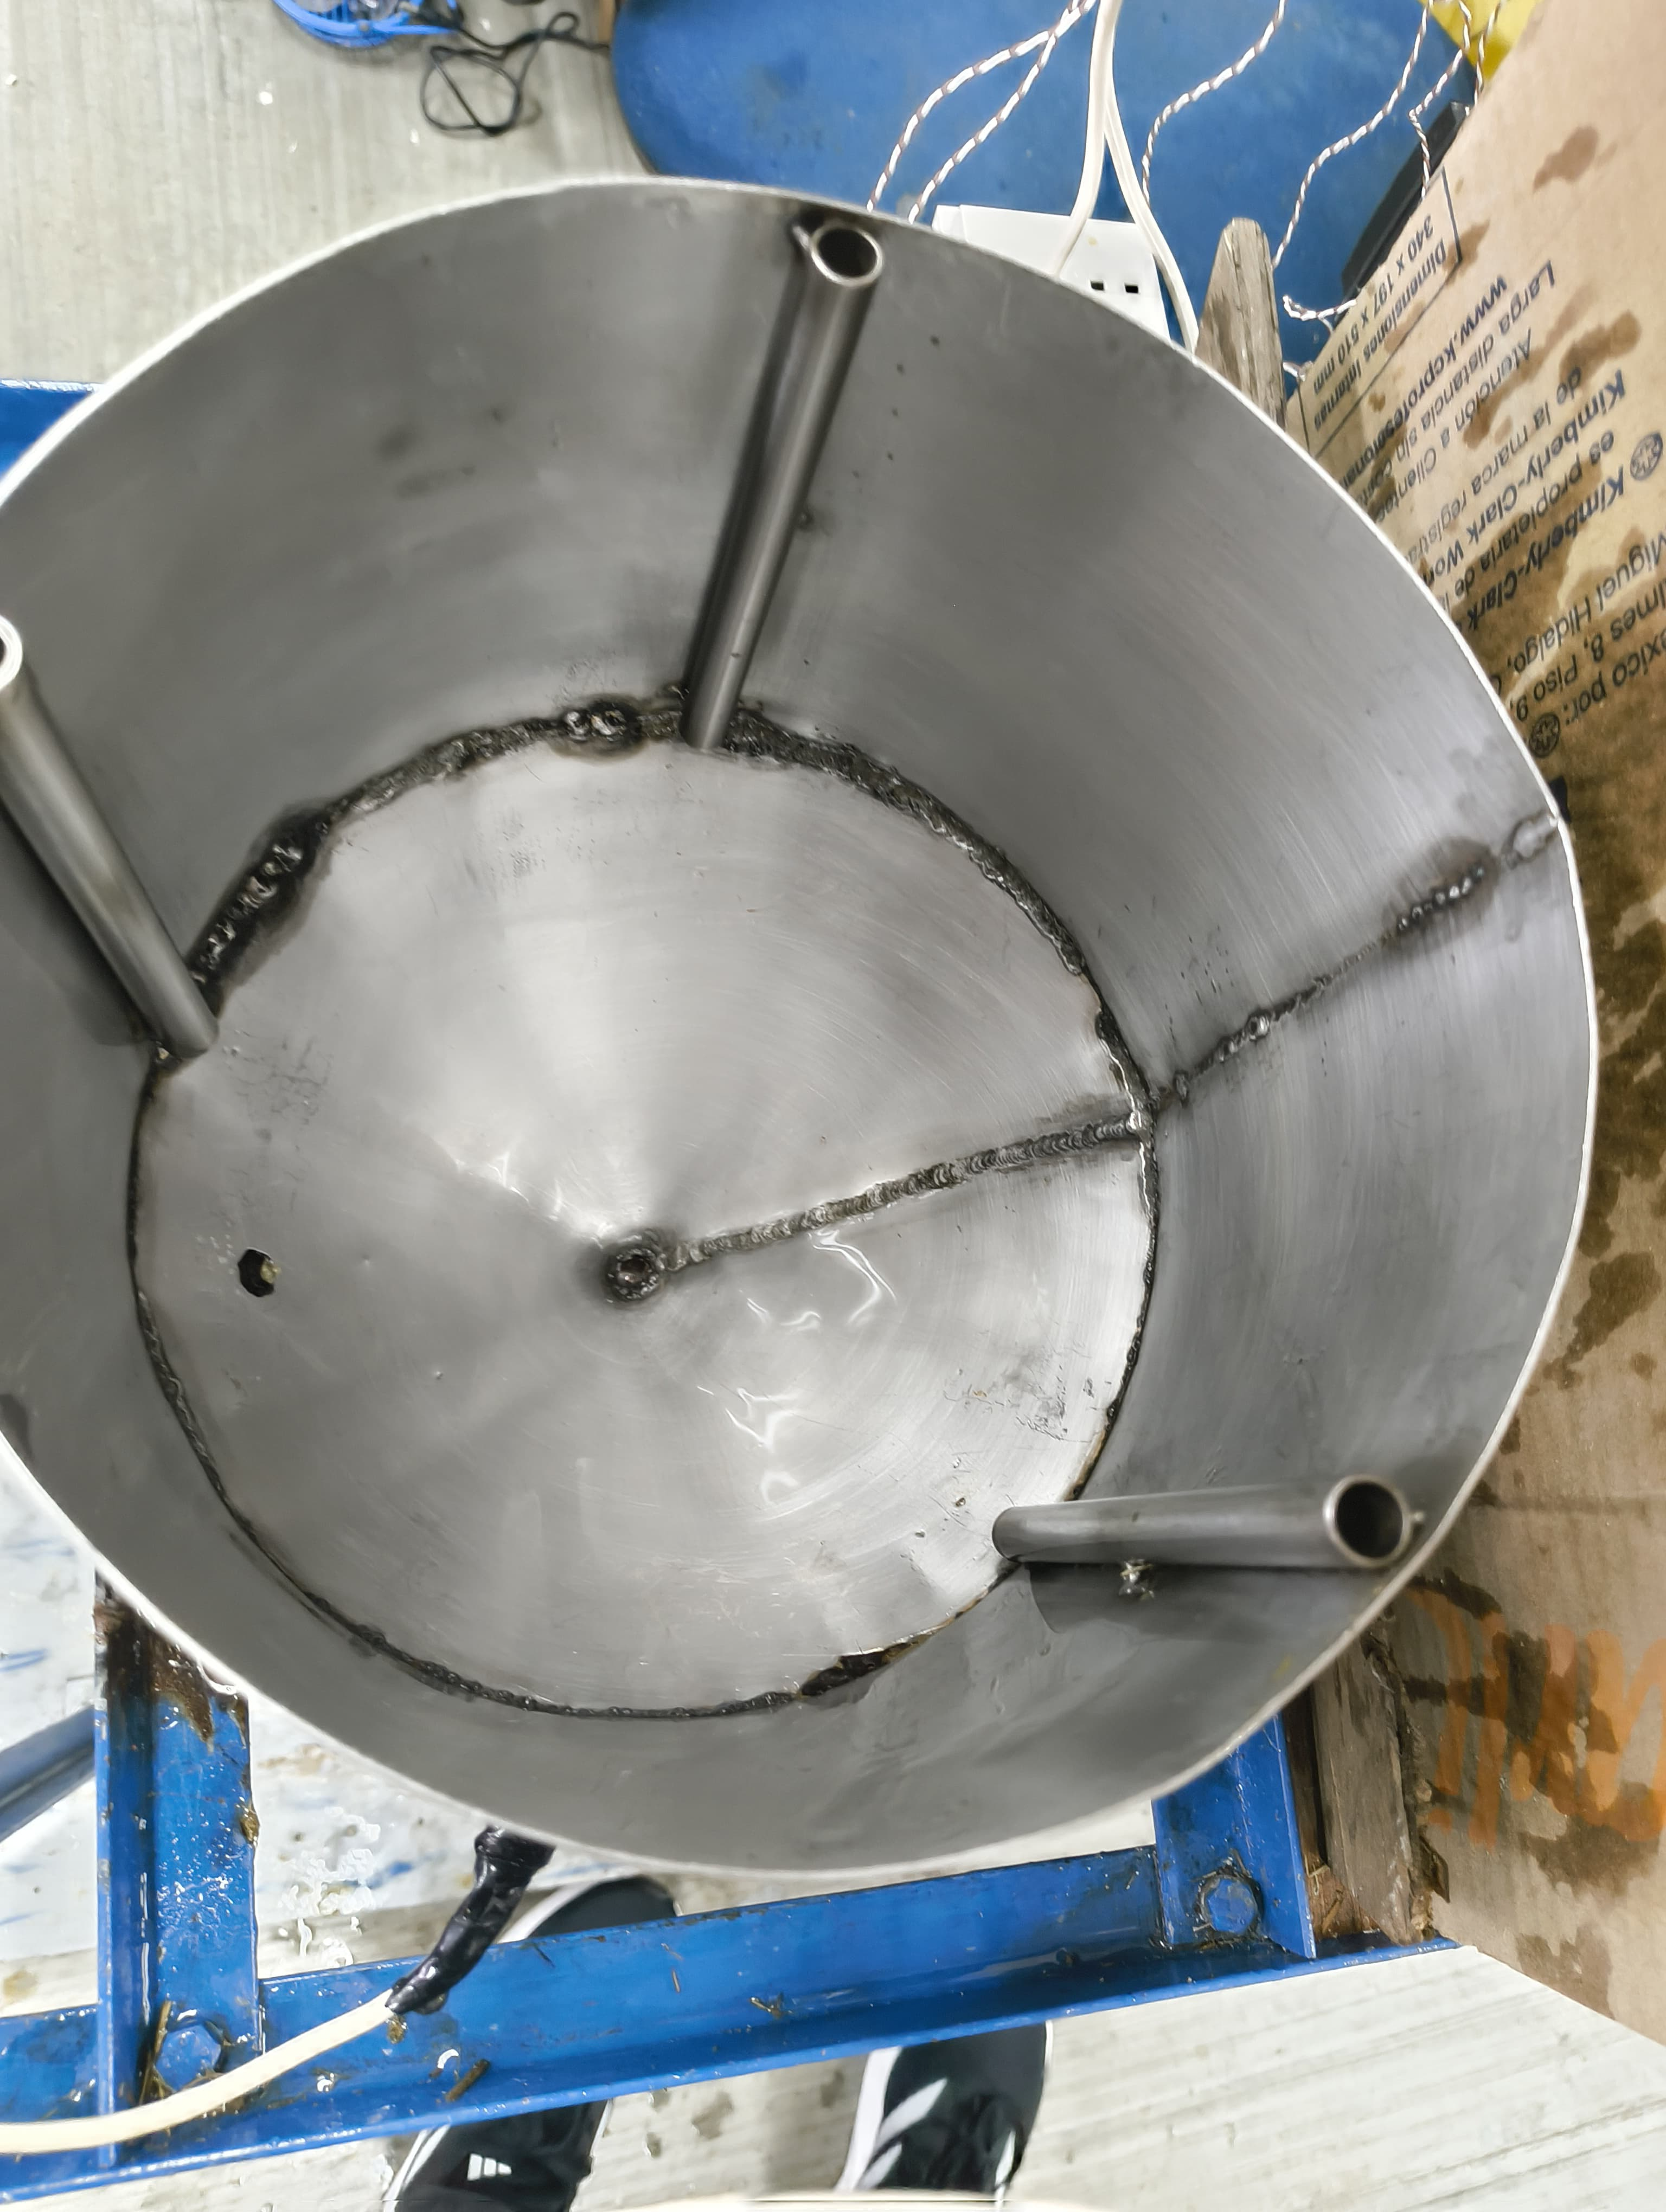
\includegraphics[width=3cm, height=5cm,angle=90]{imagenes/reactor limpio}
				\caption{Reactor previamente enjuagado con agua desmineralizada}
				\label{reactor limpio}
			\end{figure}
			
			\textbf{4.} Se procede a activar los componentes eléctricos y la resistencia, verificando su correcto funcionamiento. Posteriormente, se instala el tornillo de sellado en la base del reactor, asegurando su hermeticidad. En el interior del equipo previamente sanitizado, se incorporan el agua desmineralizada y el bagazo de caña en las proporciones establecidas, iniciando así el proceso de tratamiento. 
			
			\textbf{5.} Se incorpora el hidróxido de sodio (NaOH) previamente dosificado al reactor que contiene la mezcla de agua desmineralizada y bagazo de caña,  como se documenta en la Figura \ref{bagazo con hidroxido}.
			
			
			\begin{figure}[H]
				\centering
				\begin{minipage}{0.46\textwidth}
					\centering
					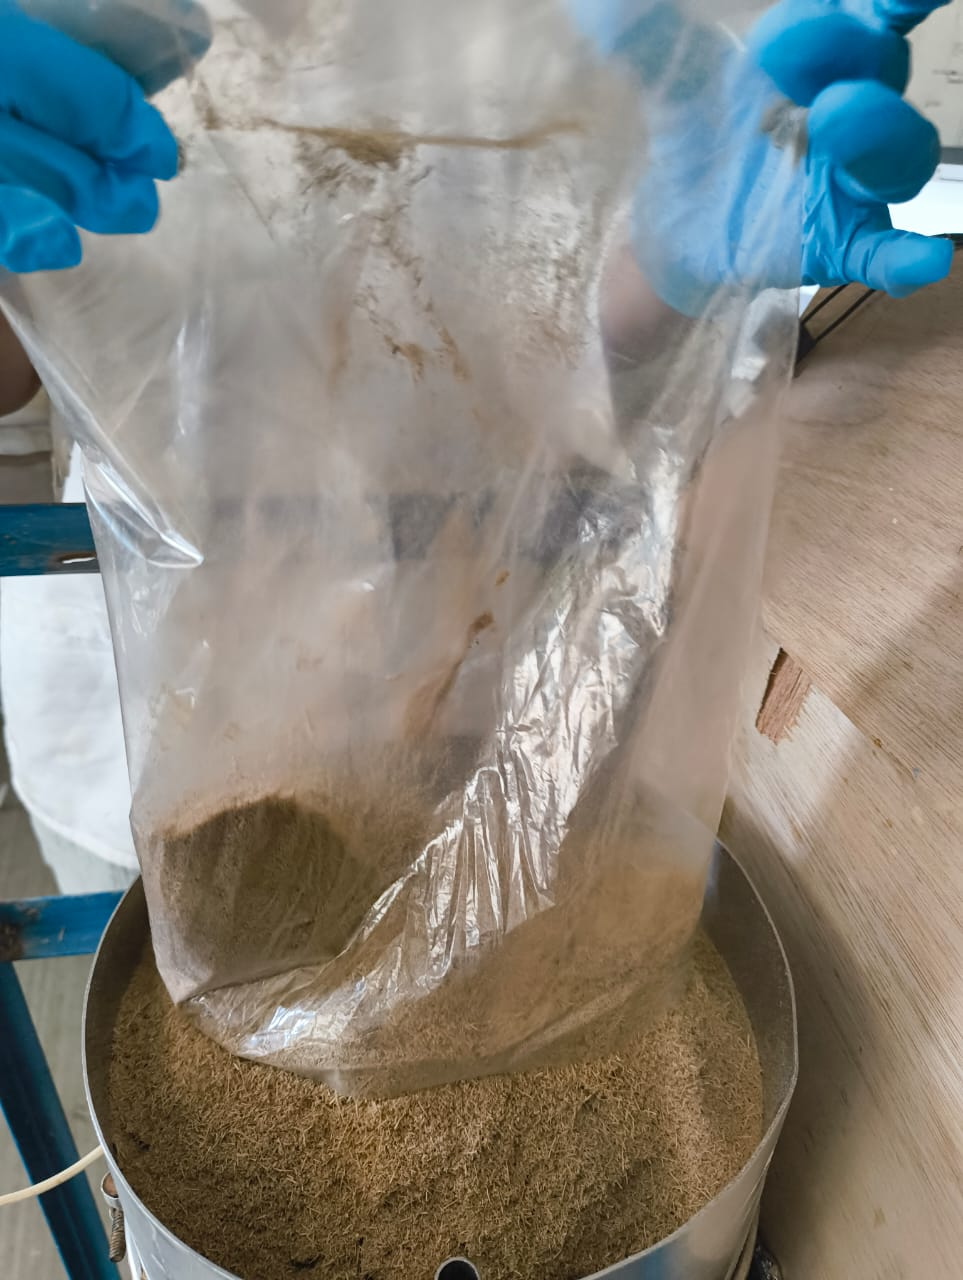
\includegraphics[width=3cm, height=3cm]{imagenes/agua con bagazo}
					\caption{Se agrega el bagazo de caña al reactor con agua desmineralizada.}
					\label{agua con bagazo}
				\end{minipage}
				\hfill
				\begin{minipage}{0.48\textwidth}
					\centering
					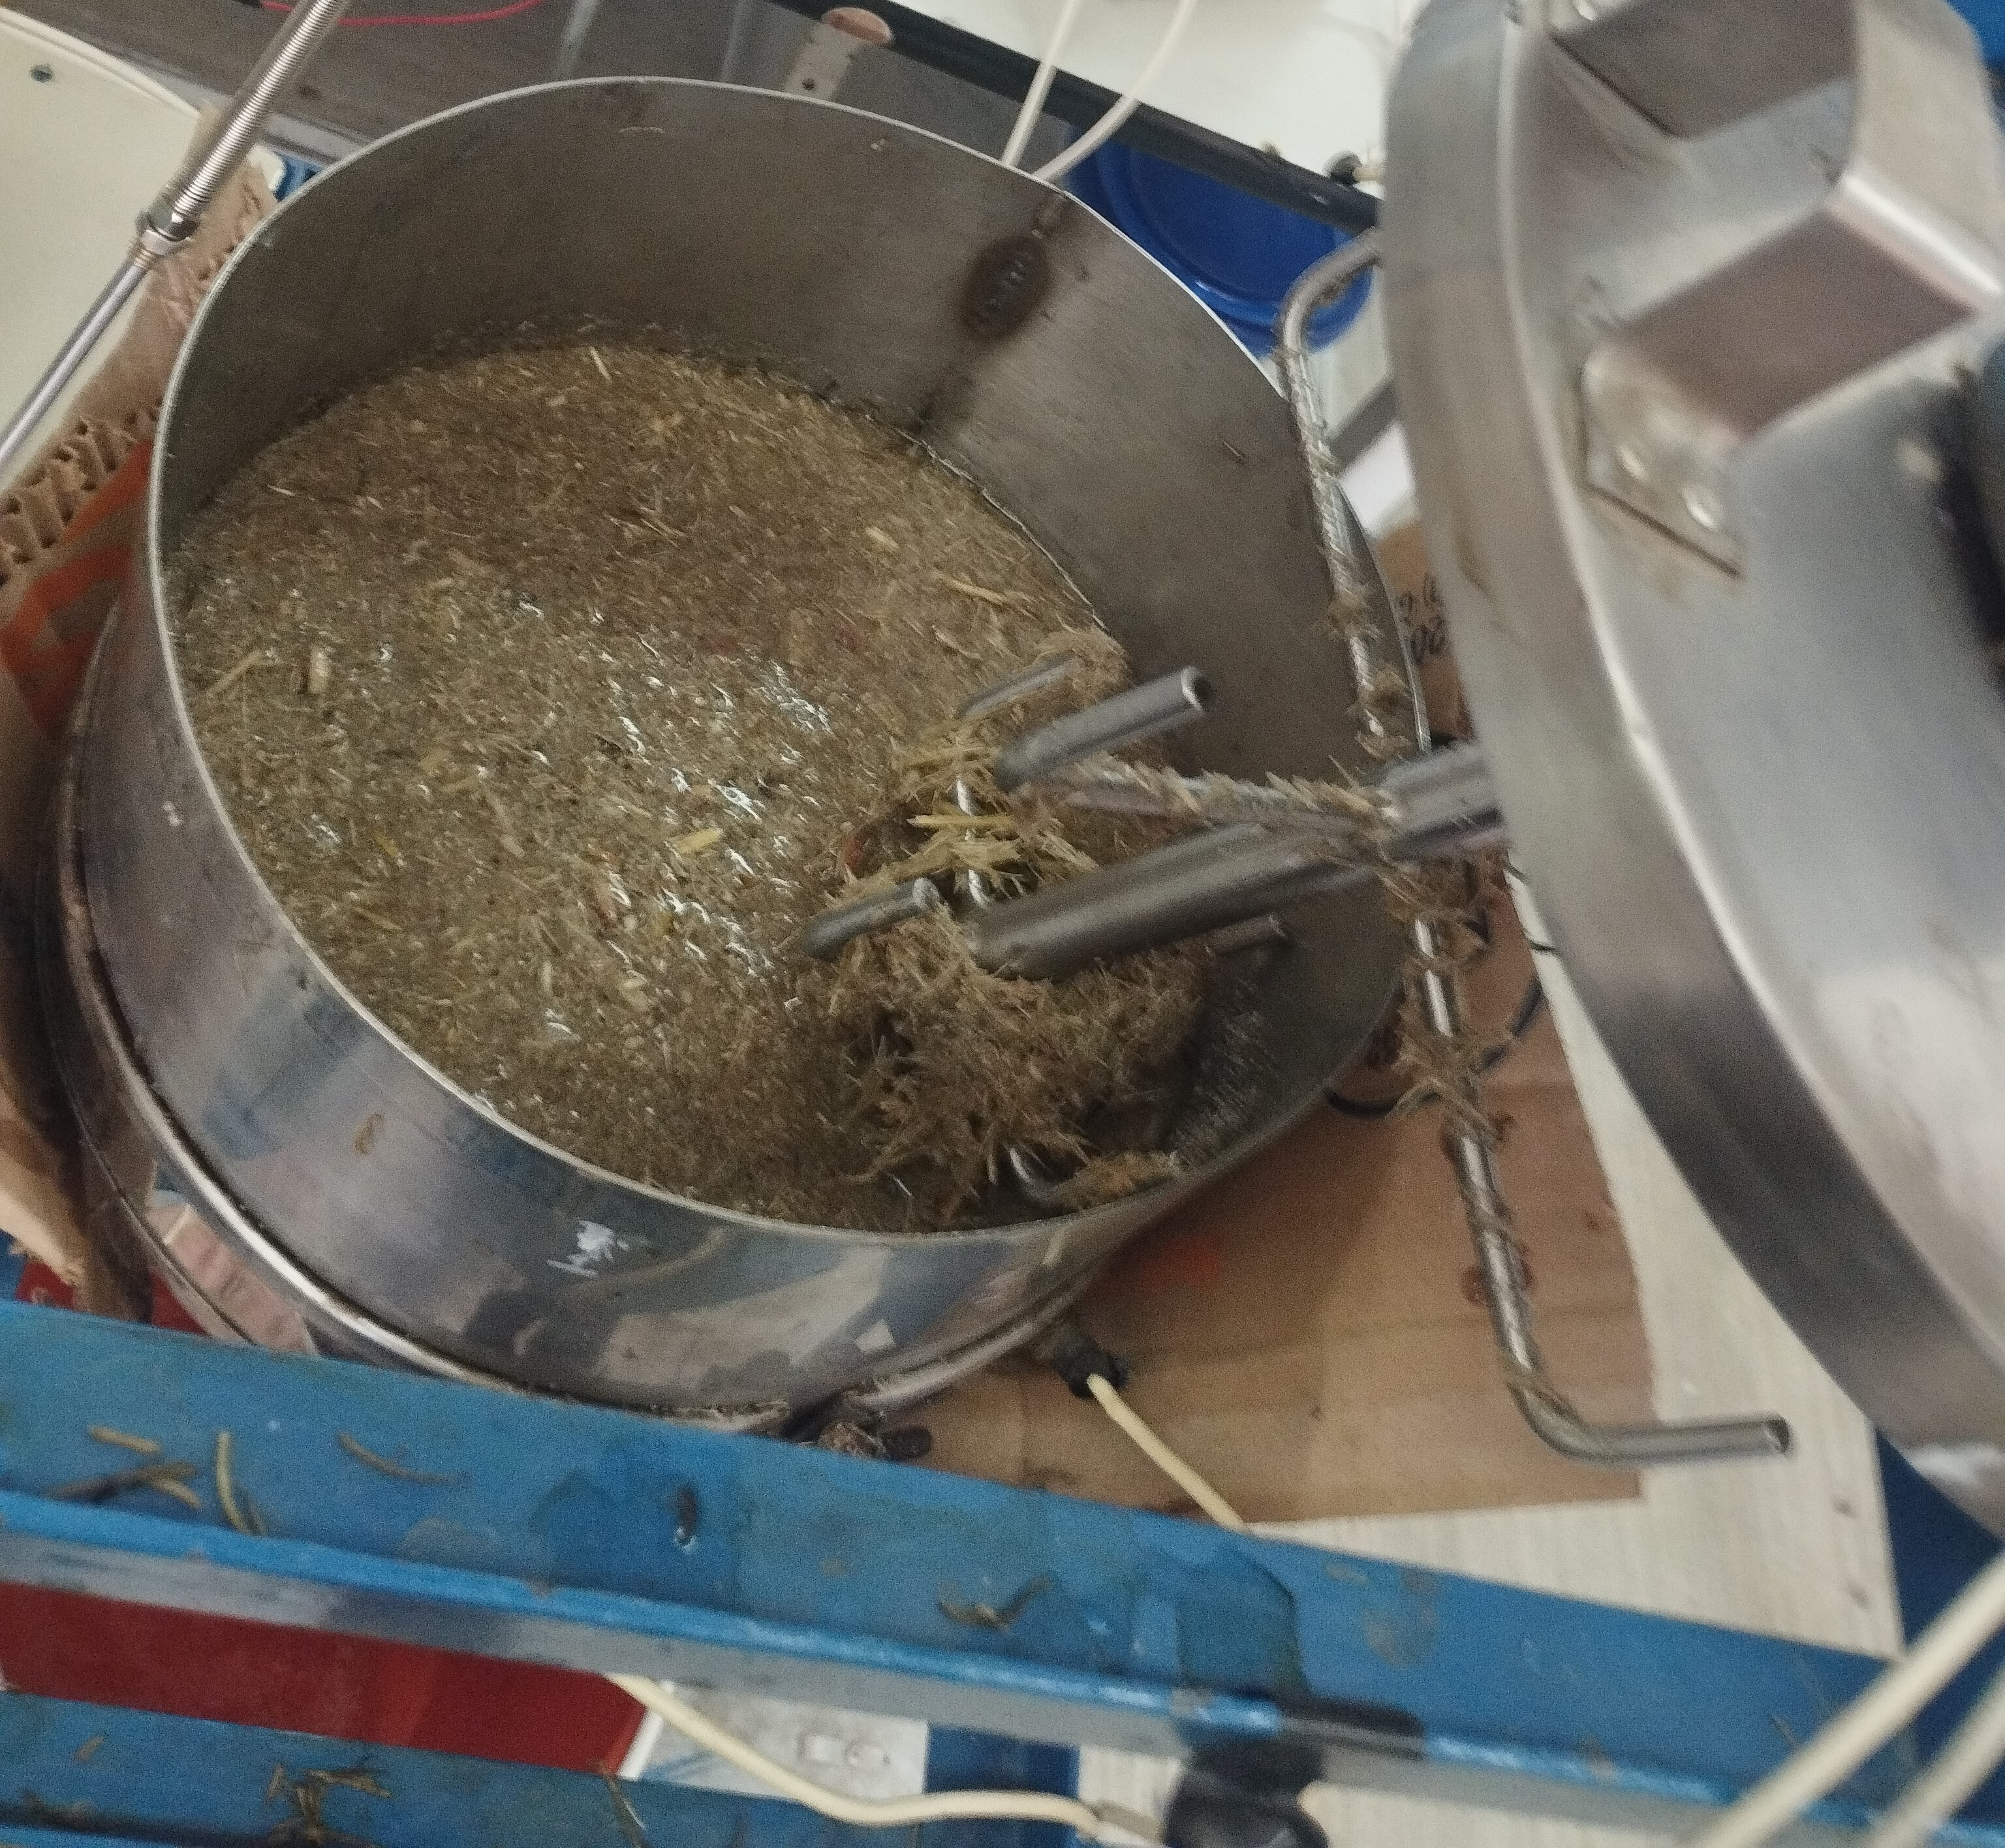
\includegraphics[width=5cm, height=3cm]{imagenes/bagazo con hidroxido1}
					\caption{Se agrega el hidróxido y se mezcla hasta incorporarse.}
					\label{bagazo con hidroxido}
				\end{minipage}
			\end{figure}
			
			
			\textbf{6.} El reactor se sella herméticamente mediante un sistema multicapa compuesto por:algodón como barrera primaria, papel aluminio para aislamiento térmico y cinta aislante/ térmica como sellado secundario, garantizando el cierre completo del sistema como se detalla en la Figura \ref{sellado_bio}.
			
			
			
			\textbf{7.} Finalmente, se activa el sistema de control automatizado (Figura \ref{programa}), implementando los perfiles programados de temperatura ambiente y tiempo de pretratamiento establecidos en el diseño experimental (Figura \ref{Diagrama1}), con el objetivo de garantizar las condiciones óptimas para el proceso.
			
			
			\begin{figure}[H]
				\centering
				\begin{minipage}{0.46\textwidth}
					\centering
					\includegraphics[width=\linewidth, height=4cm, keepaspectratio]{imagenes/sellado2}
					\caption{El reactor se sella con ayuda de algodón, papel aluminio y cinta de aislar o cinta térmica.}
					\label{sellado_bio}
				\end{minipage}
				\hfill
				\begin{minipage}{0.48\textwidth}
					\centering
					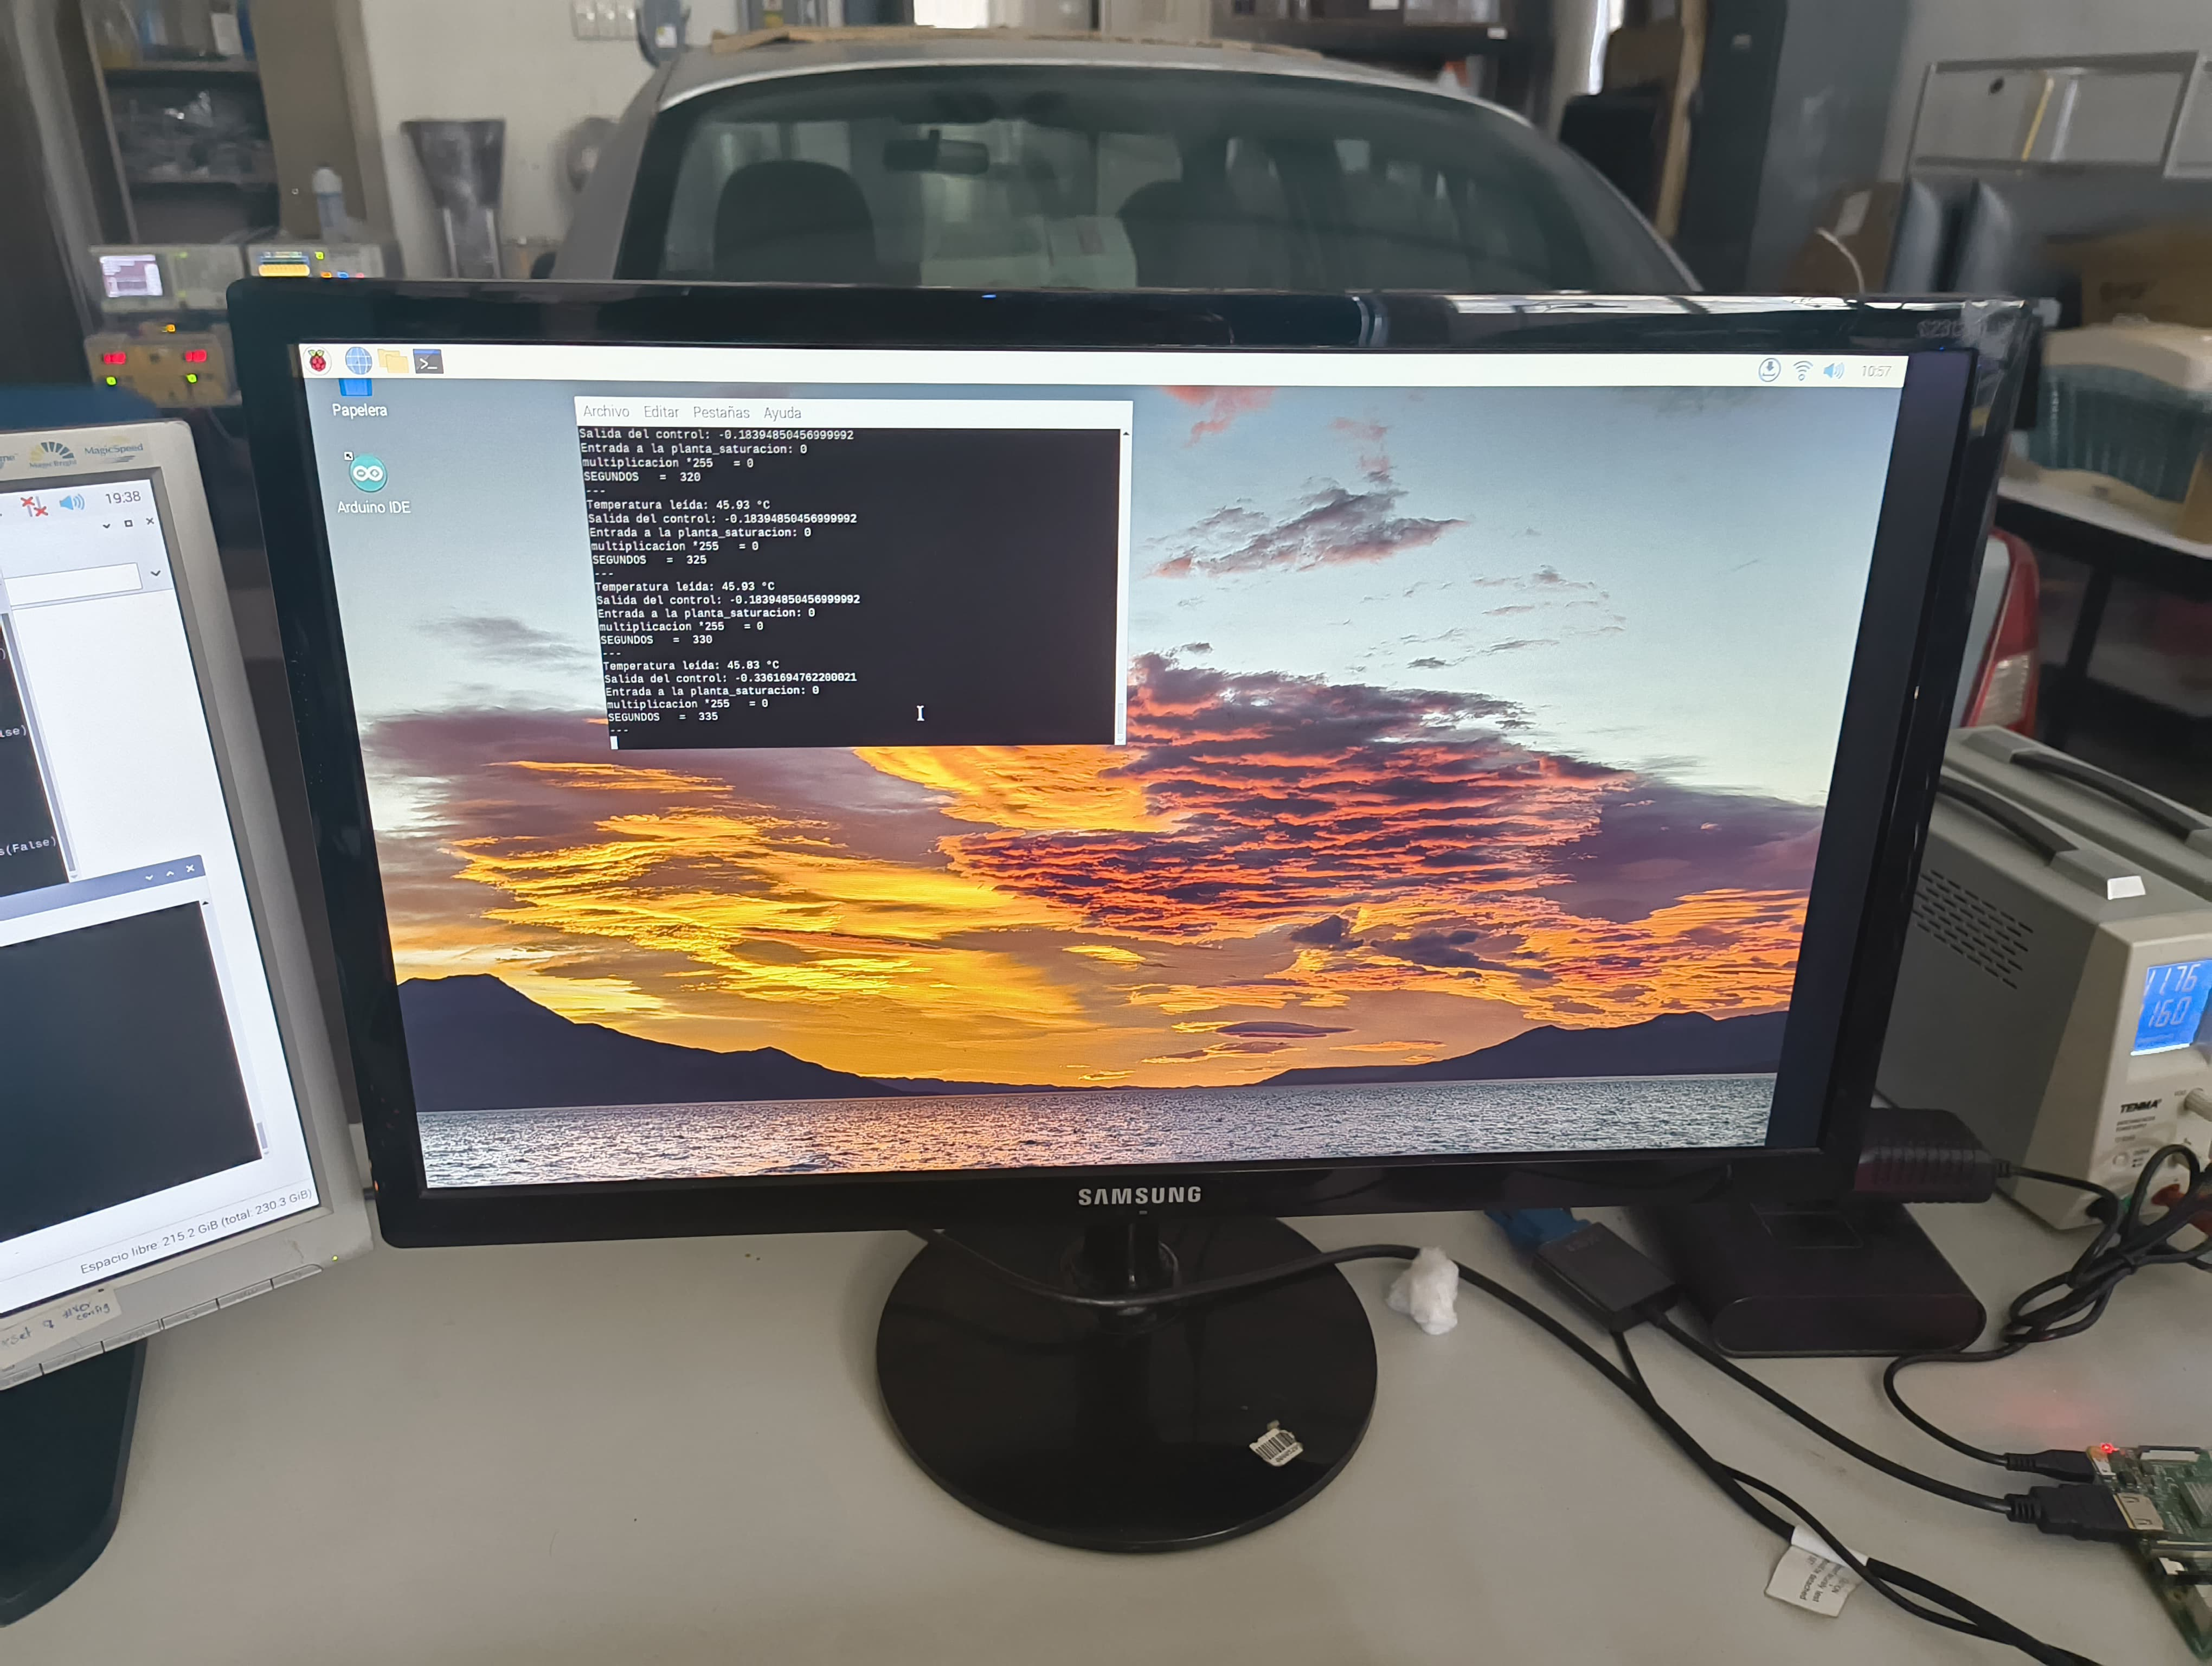
\includegraphics[width=\linewidth, height=4cm, keepaspectratio]{imagenes/programa3}
					\caption{Se muestra el programa en funcionamiento.}
					\label{programa}
				\end{minipage}
			\end{figure}
			
			\textbf{7.} El diseño del control de la temperatura podemos observarla en el anexo \ref{diseño del control de temp}
			
			%%%%%%%%%%%%%%%%%%%%%%%%%%%%%%%%%%%%%%%%%%%%%%%%%%%%%%%%%%%%%%%%%%%%%%%%%%%%%%%%%%%%%%%%%%%%%%%%%%%%%%%%%%%%%%%%%%%%%%%%%%%%%%%%%%%%%%%%%%%%%%%%%%%%%%%%%%%%%\t
			
			
			
			\subsubsection{Acondicionamiento para el material pretratado}
			
			 \textbf{Materiales}
			\\[0.5em]
		
			\begin{tabular}{p{0.3\textwidth}p{0.3\textwidth}p{0.3\textwidth}}
				$\bullet$ \textit{Agua desmineralizada} & $\bullet$ \textit{ Bagazo de caña Pretratado} & $\bullet$ \textit{Tela delgada}  \\
			
				$\bullet$ \textit{Colador} & $\bullet$ \textit{Cubeta 10 l} & 
			\end{tabular}
			\\[0.5em]
			
			
			\textbf{Procedimiento}
			\\[0.5em] 
			\textbf{1.} Durante el pretratamiento biológico, se registran periódicamente los datos experimentales para garantizar su trazabilidad, y al finalizar el proceso se almacena toda la información recopilada. Adicionalmente, se registra el consumo energético mediante la lectura del watímetro (Figura \ref{watimetro}), el cual cuantifica la energía utilizada en kilovatios-hora (kWh) a lo largo del tratamiento.
			
			
			\textbf{2.} Bajo condiciones controladas, se desarma el sistema retirando primero los elementos de sellado (aluminio/algodón), luego los componentes electrónicos (sensores termopares tipo k) y finalmente el conjunto tapa-mezclador, dejando la configuración documentada en la Figura \ref{biologico1}.
	
			
					
			\begin{figure}[H]
				\centering
				\begin{minipage}{0.46\textwidth}
					\centering
					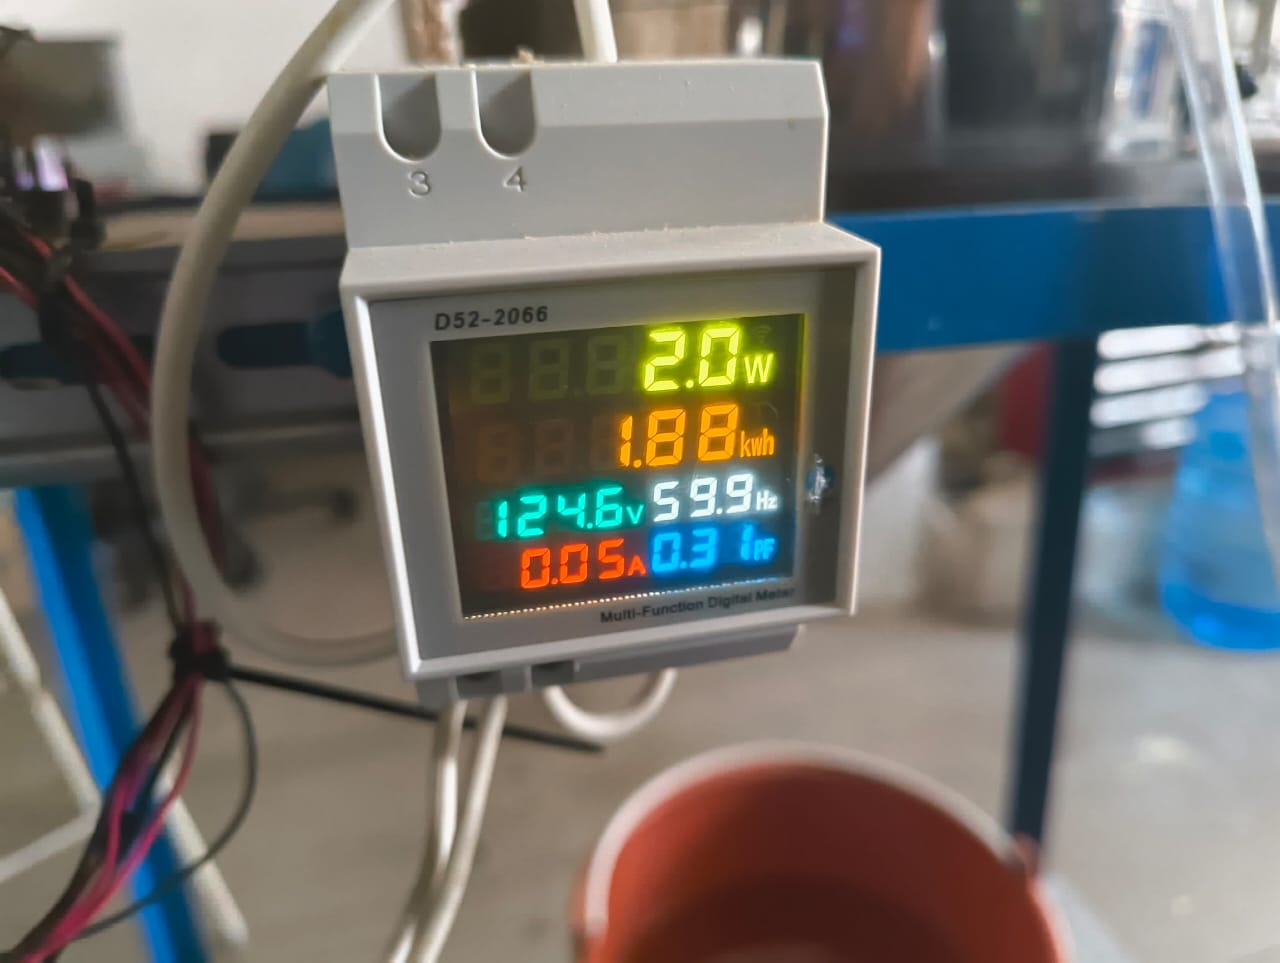
\includegraphics[width=5cm, height=3cm]{imagenes/watimetro} % Cambia "imagen1.jpg" por el nombre de tu archivo
					\caption{Se observa el watimetro que se encuentra en la estructura y mide la energia que entra al convertidor.}
						\label{watimetro}
					\end{minipage}
					\hfill
					\begin{minipage}{0.48\textwidth}
						\centering
						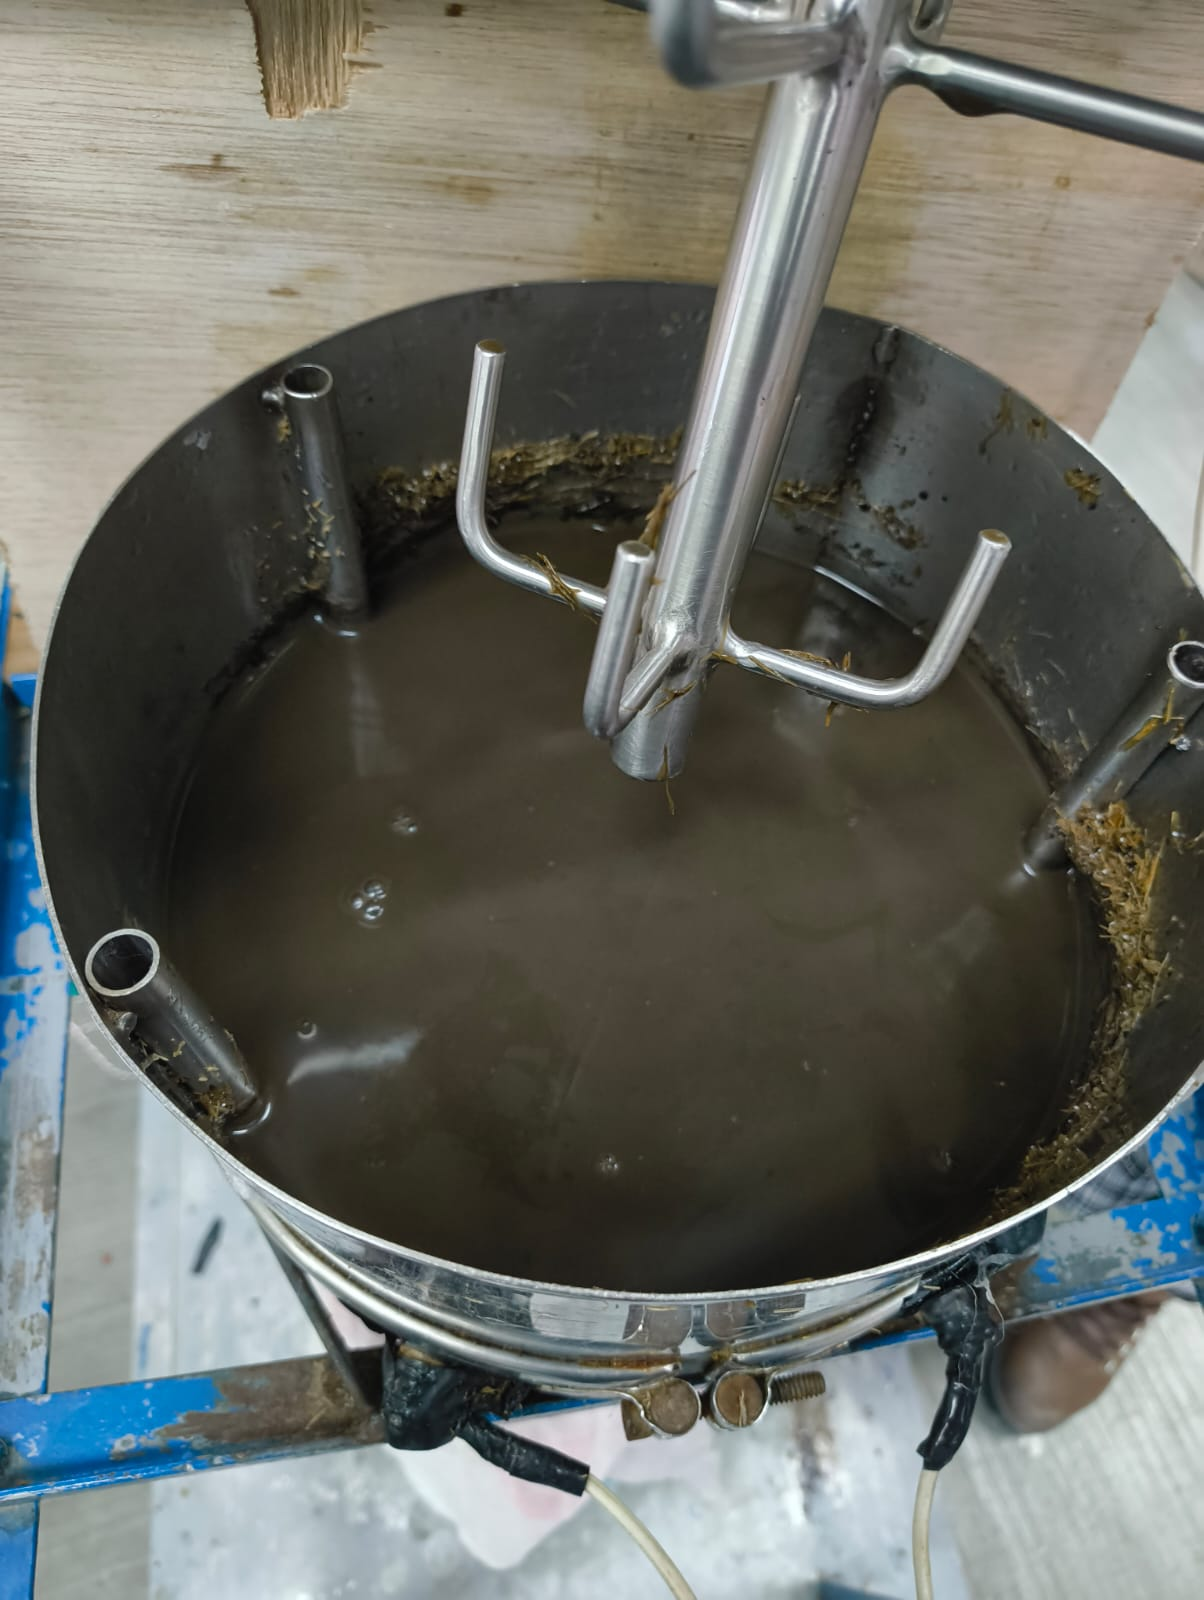
\includegraphics[width=4cm, height=3cm]{imagenes/biologico1} % Cambia "imagen2.jpg" por el nombre de tu archivo
						\caption{Se observa el watimetro que se encuentra en la estructura y mide la energia que entra al convertidor.}
						\label{biologico1}
					\end{minipage}
				\end{figure}
				
			
			\textbf{3.} Para la separación sólido-líquido, se implementa un sistema de filtración compuesto por una cubeta de 10 L que integra una manta filtrante y un colador (Figura \ref{Cubeta con colador y manta para colar el bagazo pretratado.}). En este dispositivo se coloca el bagazo pretratado, permitiendo la retención de la biomasa y el paso del liquido resultante, tal como se documenta en la Figura \ref{Bagazo1}.
 
				\begin{figure}[H]
				\centering
				\begin{minipage}{0.46\textwidth}
					\centering
					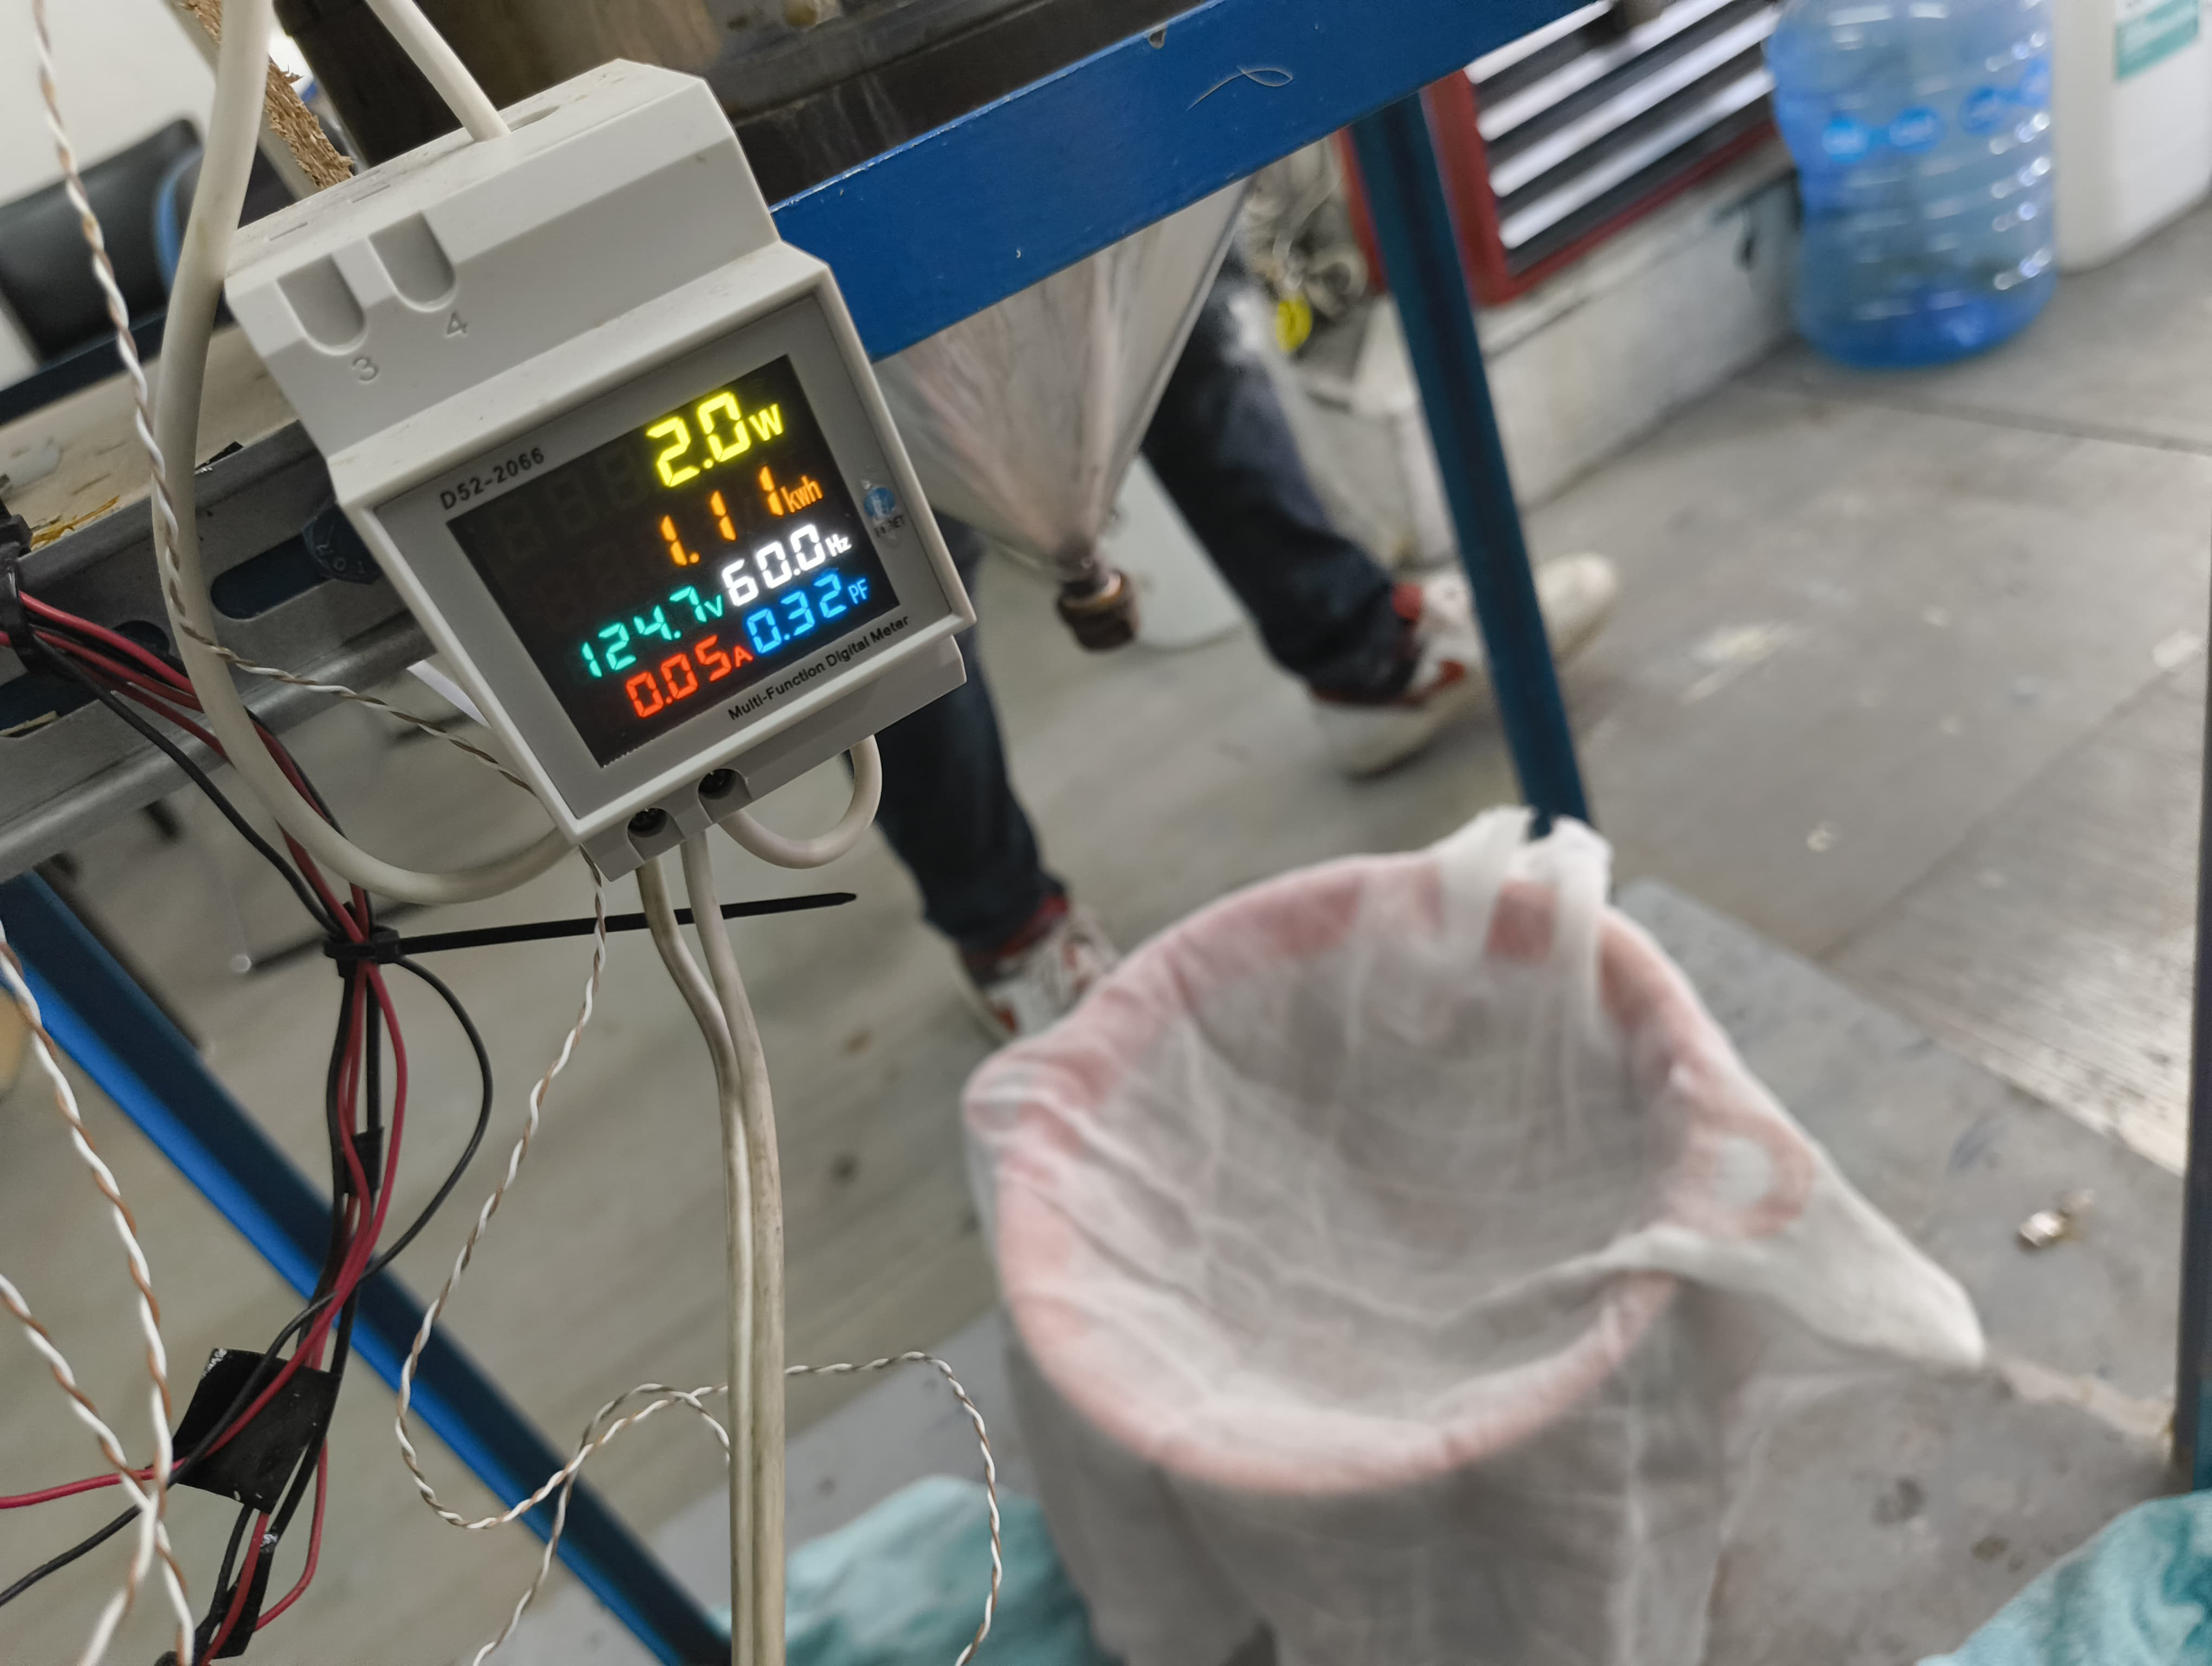
\includegraphics[width=5cm, height=3cm]{imagenes/biologico6} % Cambia "imagen1.jpg" por el nombre de tu archivo
					\caption{Cubeta con colador y manta para colar el bagazo pretratado.}
					\label{Cubeta con colador y manta para colar el bagazo pretratado.}
				\end{minipage}
				\hfill
				\begin{minipage}{0.48\textwidth}
					\centering
					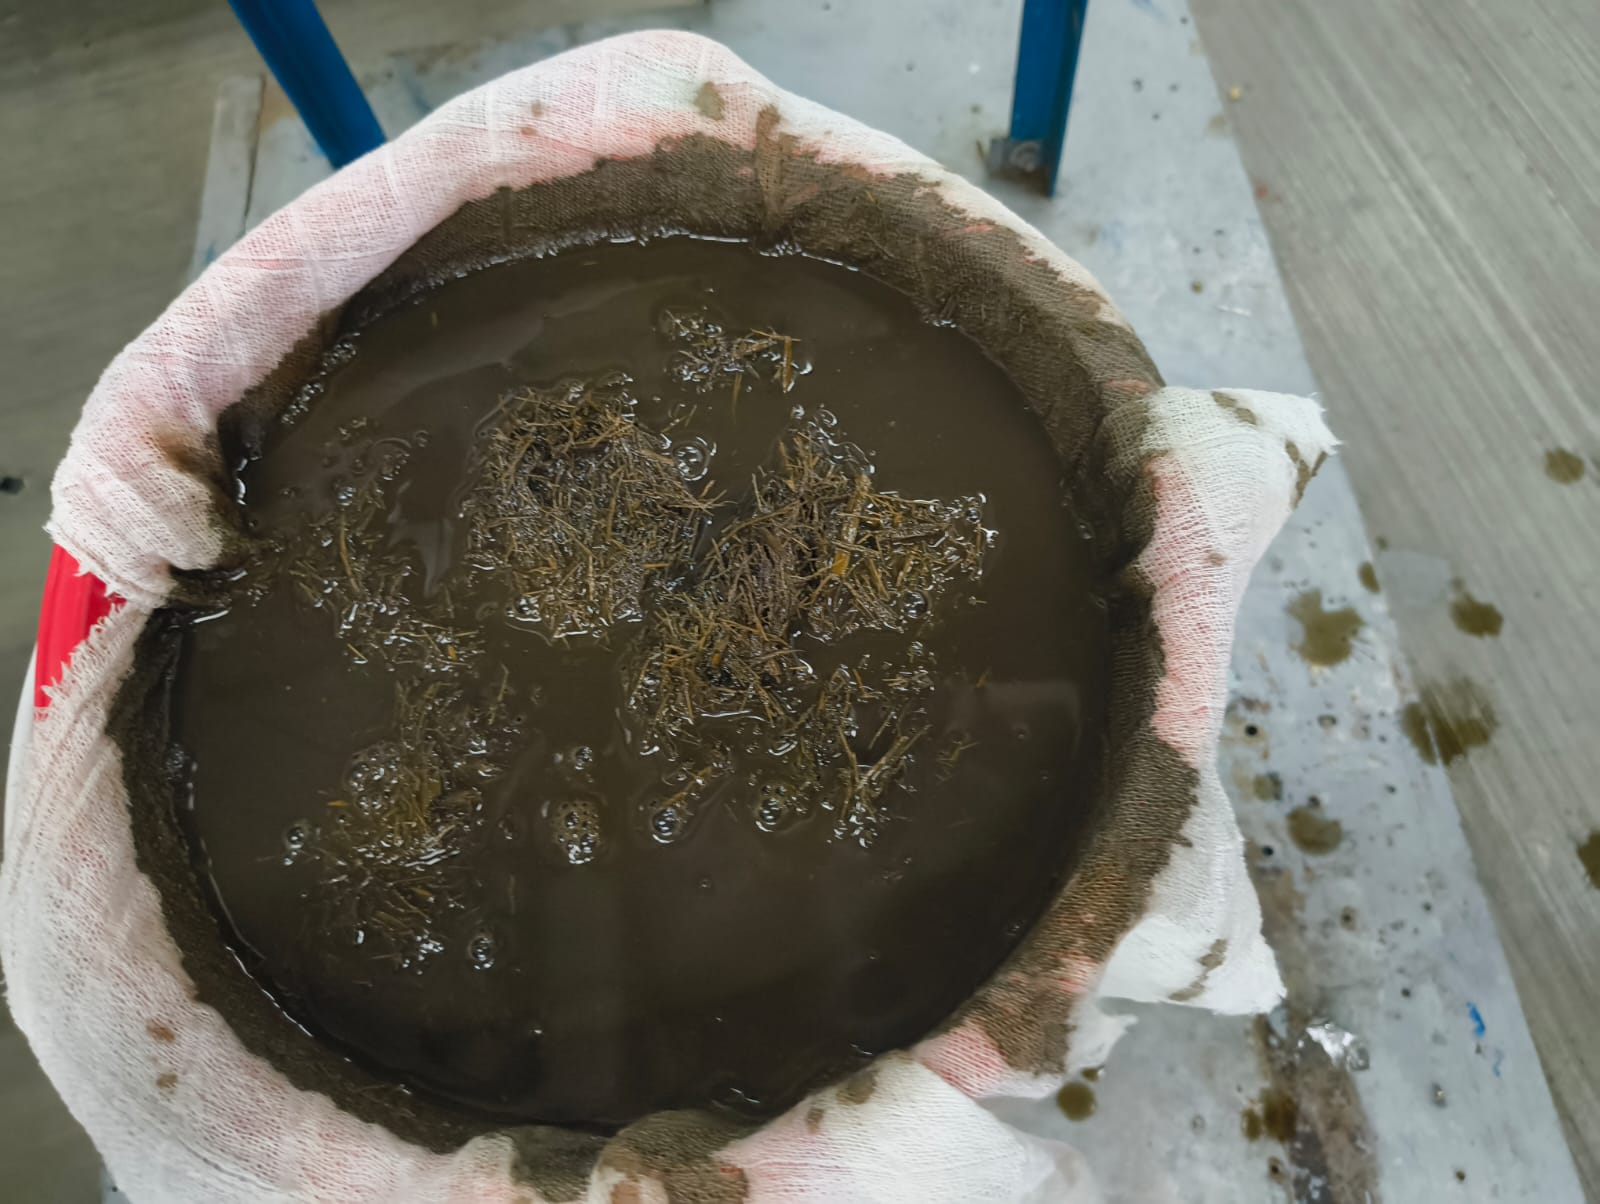
\includegraphics[width=5cm, height=3cm]{imagenes/bagazo_biologico_sacado} % Cambia "imagen2.jpg" por el nombre de tu archivo
					\caption{Bagazo previamente pretratado.}
					\label{Bagazo1}
				\end{minipage}
			\end{figure}
	
	     \textbf{4.} El bagazo pretratado se mantiene en la cubeta hasta completar el filtrado del agua residual, tras lo cual se somete a un proceso de lavado con agua adicional para eliminar el máximo posible de humus de lombriz o el hidróxido de sodio respectivamente. Posteriormente, el material se exprime manualmente para extraer el exceso de líquido y se deja escurrir, siguiendo el procedimiento ilustrado en la Figura \ref{biologico3}.
	     
	
	\textbf{5.} Para eliminar la humedad residual, el bagazo se extiende uniformemente en una bandeja y se introduce en un horno, donde se seca bajo condiciones controladas hasta alcanzar el contenido de humedad deseado, optimizando así el tiempo de proceso como se muestra en la Figura \ref{secado2}. 
	
	
	

	
		\begin{figure}[H]
		\centering
		\begin{minipage}{0.46\textwidth}
			\centering
			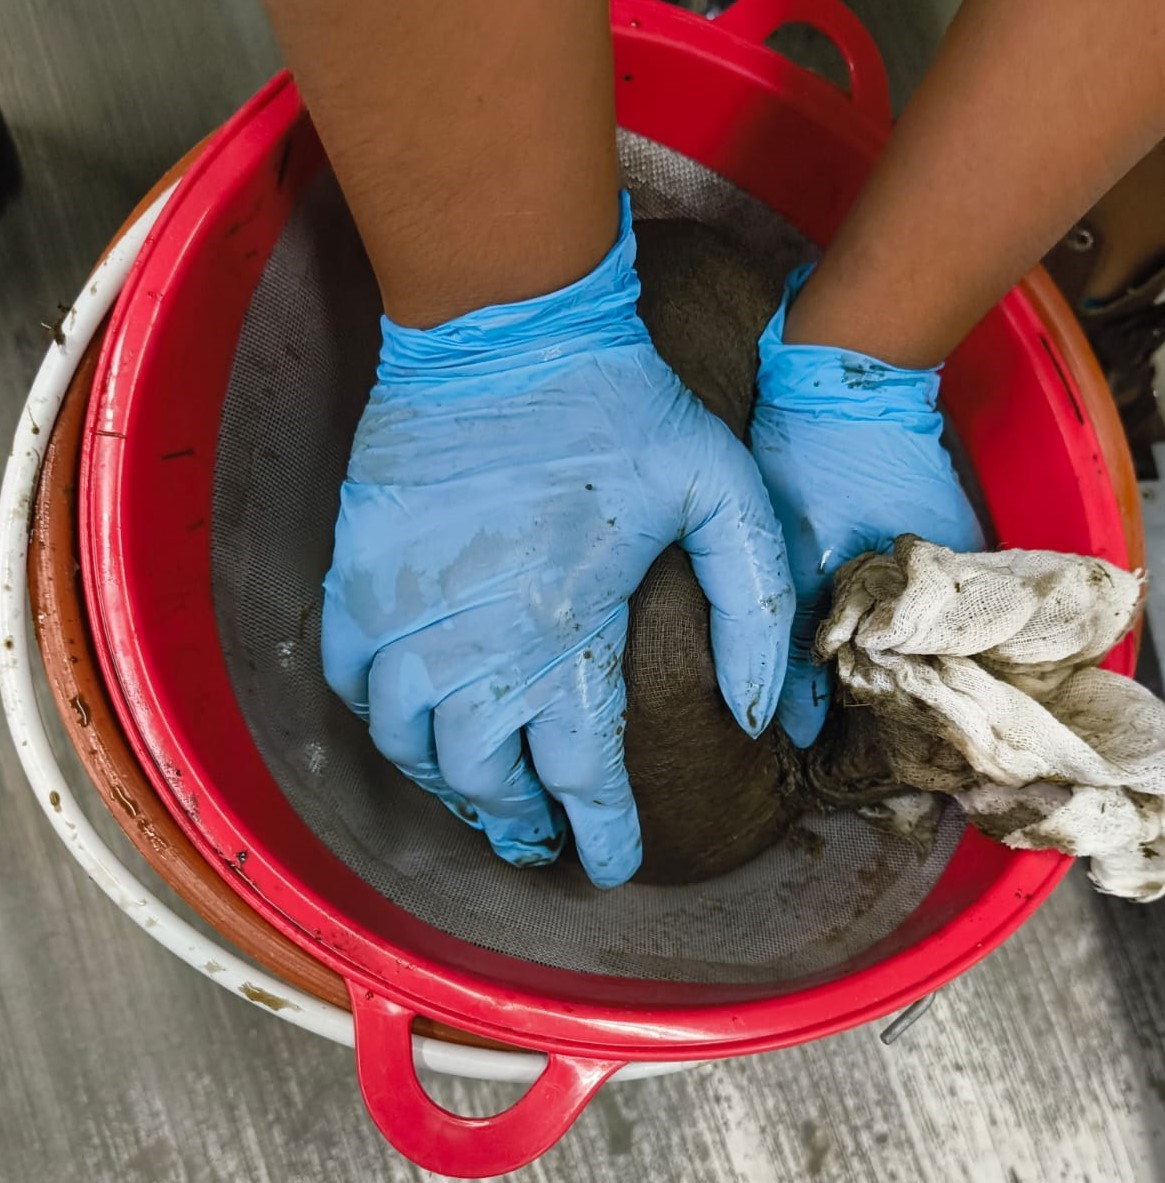
\includegraphics[width=5cm, height=3cm]{imagenes/biologico3} % Cambia "imagen1.jpg" por el nombre de tu archivo
			\caption{En la fotografía muestra como se retira el exceso de agua exprimiendo.}
			\label{biologico3}
		\end{minipage}
		\hfill
		\begin{minipage}{0.48\textwidth}
			\centering
			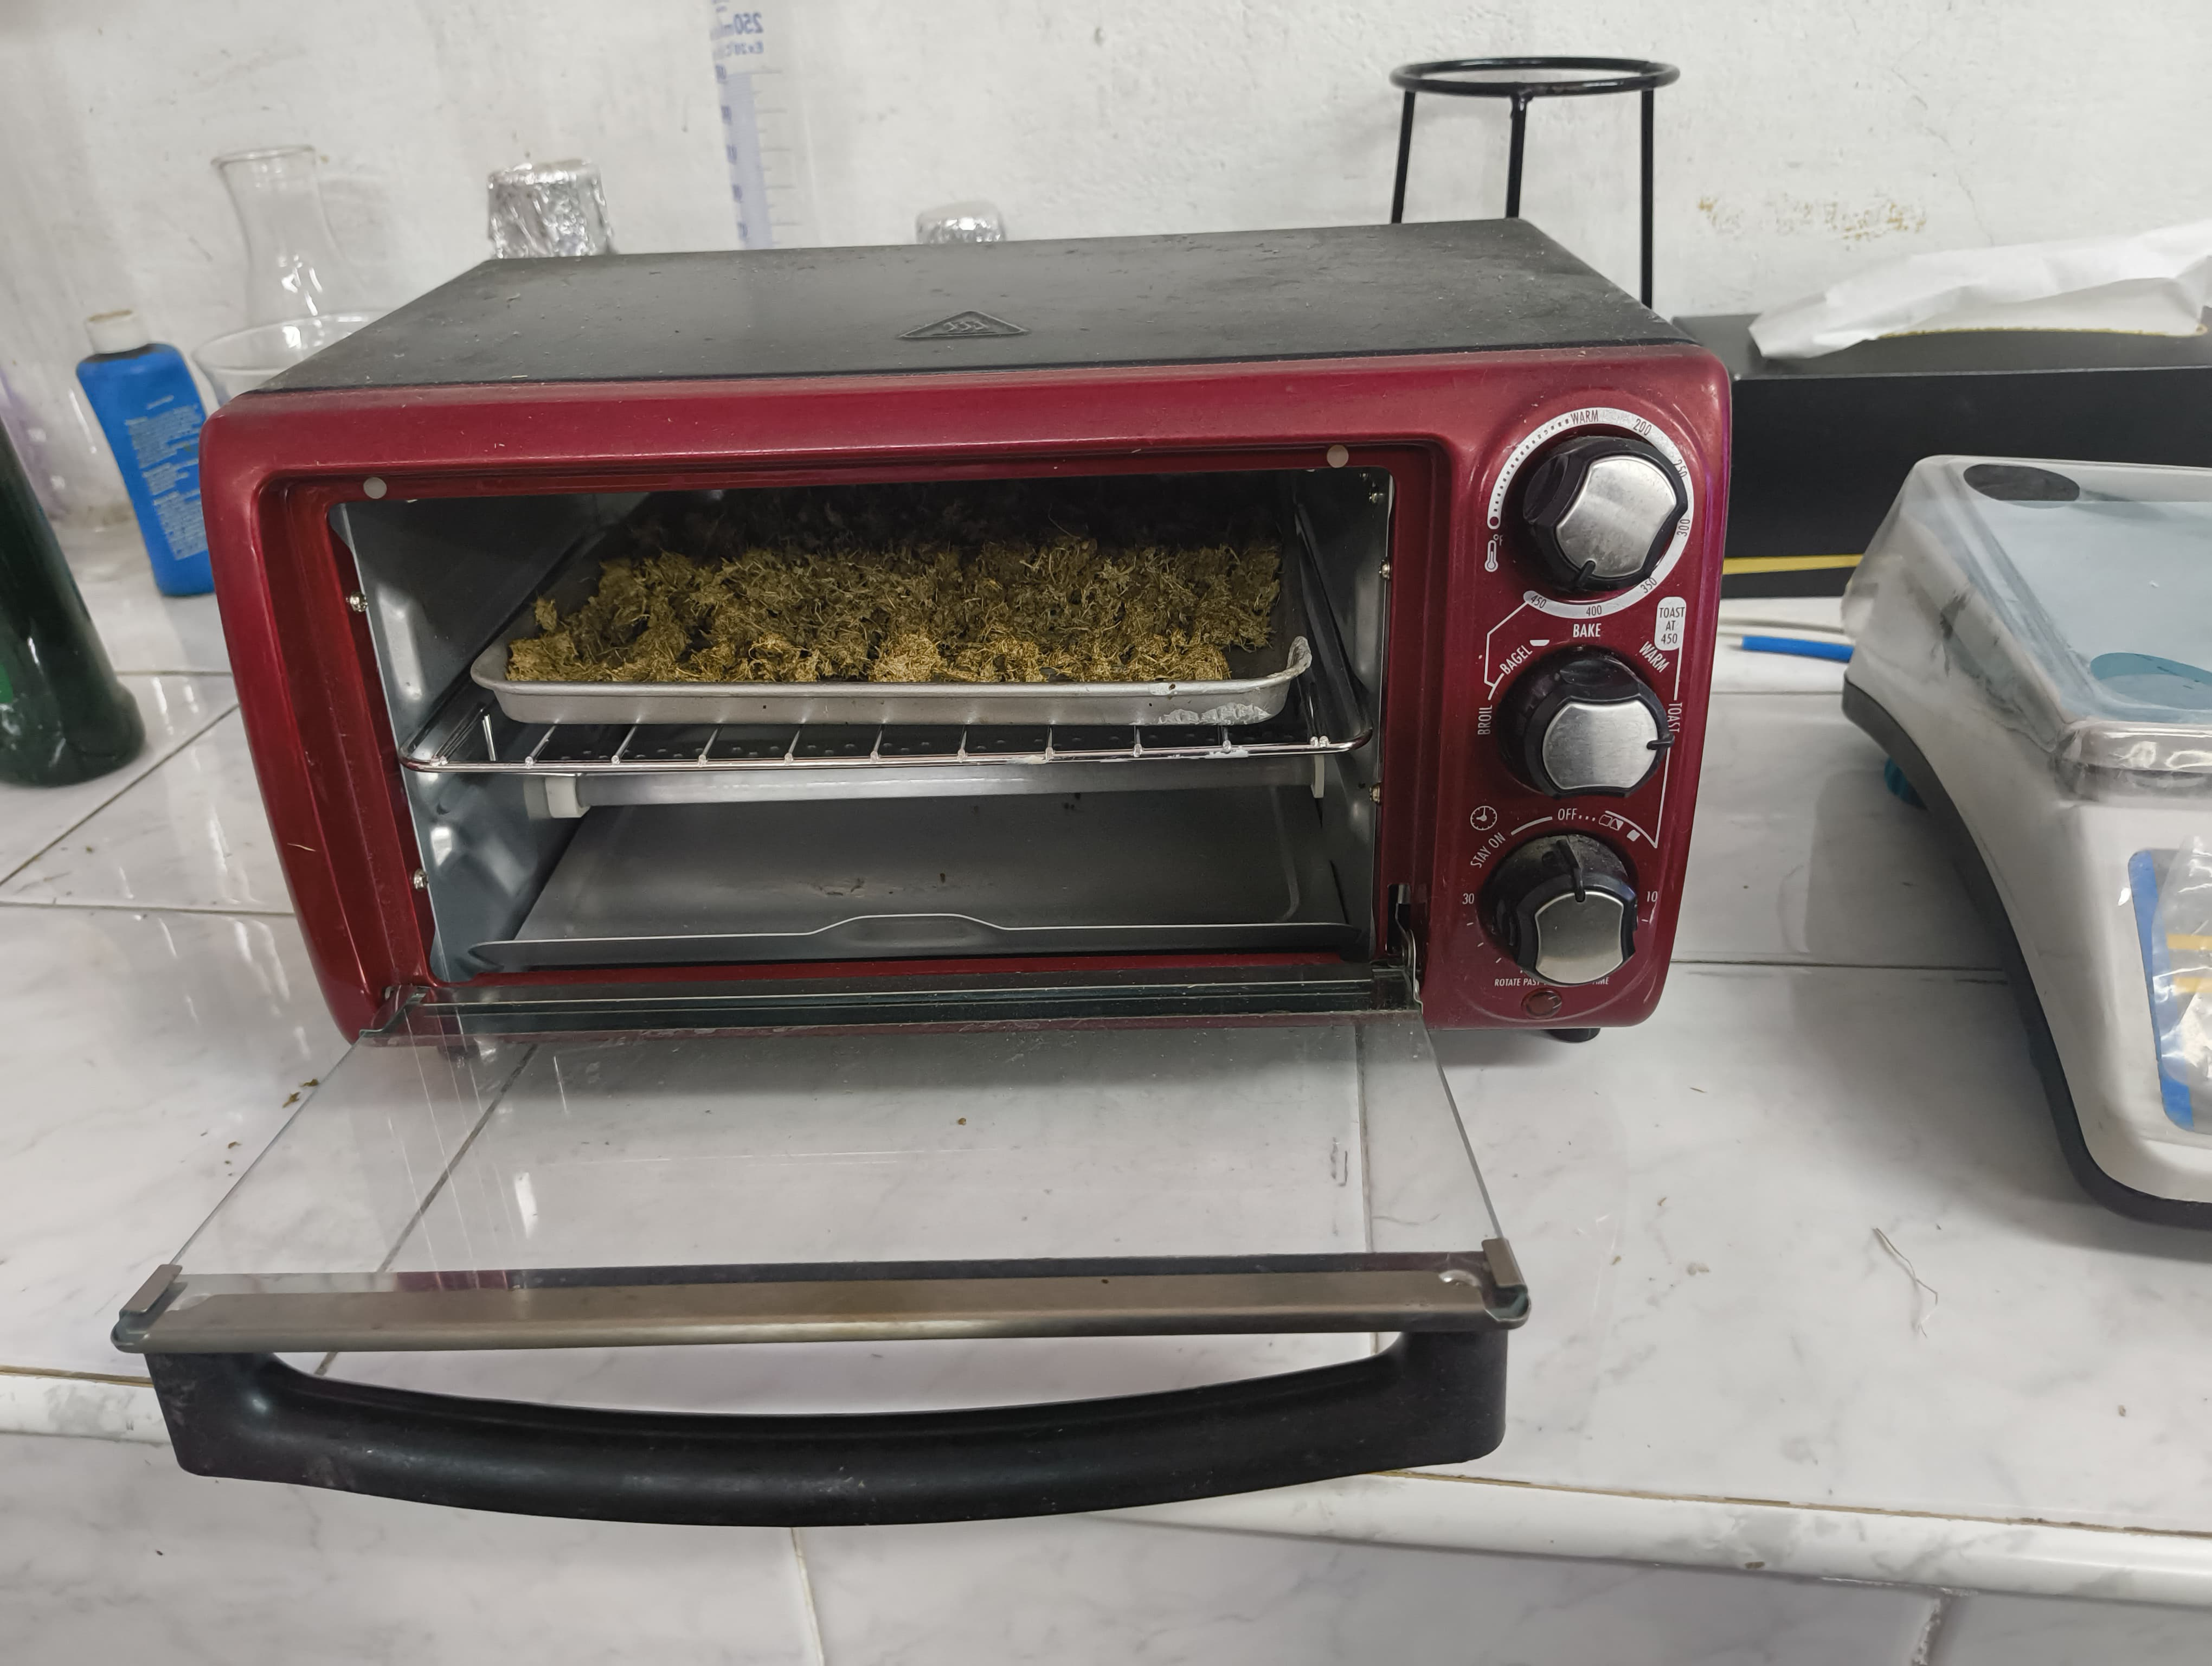
\includegraphics[width=4cm, height=3cm]{imagenes/secado2} % Cambia "imagen2.jpg" por el nombre de tu archivo
			\caption{El bagazo es secado en un horno.}
			\label{secado2}
		\end{minipage}
	\end{figure}
	
	
	
		\textbf{6.} Tras el secado inicial, el bagazo se coloca nuevamente en el colador para someterlo a un segundo enjuague con agua desmineralizada, asegurando la eliminación de residuos solubles (humus de lombriz o hidróxido de sodio), proceso que se documenta en la Figura \ref{enjuagado}.
		
	
		
	  \textbf{7.}Tras el escurrido manual, el material se somete a secado pasivo en condiciones ambientales (25 ± 2°C, humedad relativa menor a 60\%) hasta obtener peso constante, verificando la eliminación completa de humedad según se especifica en la Figura \ref{biologico4}.
	
	
		\begin{figure}[H]
		\centering
		\begin{minipage}{0.46\textwidth}
			\centering
			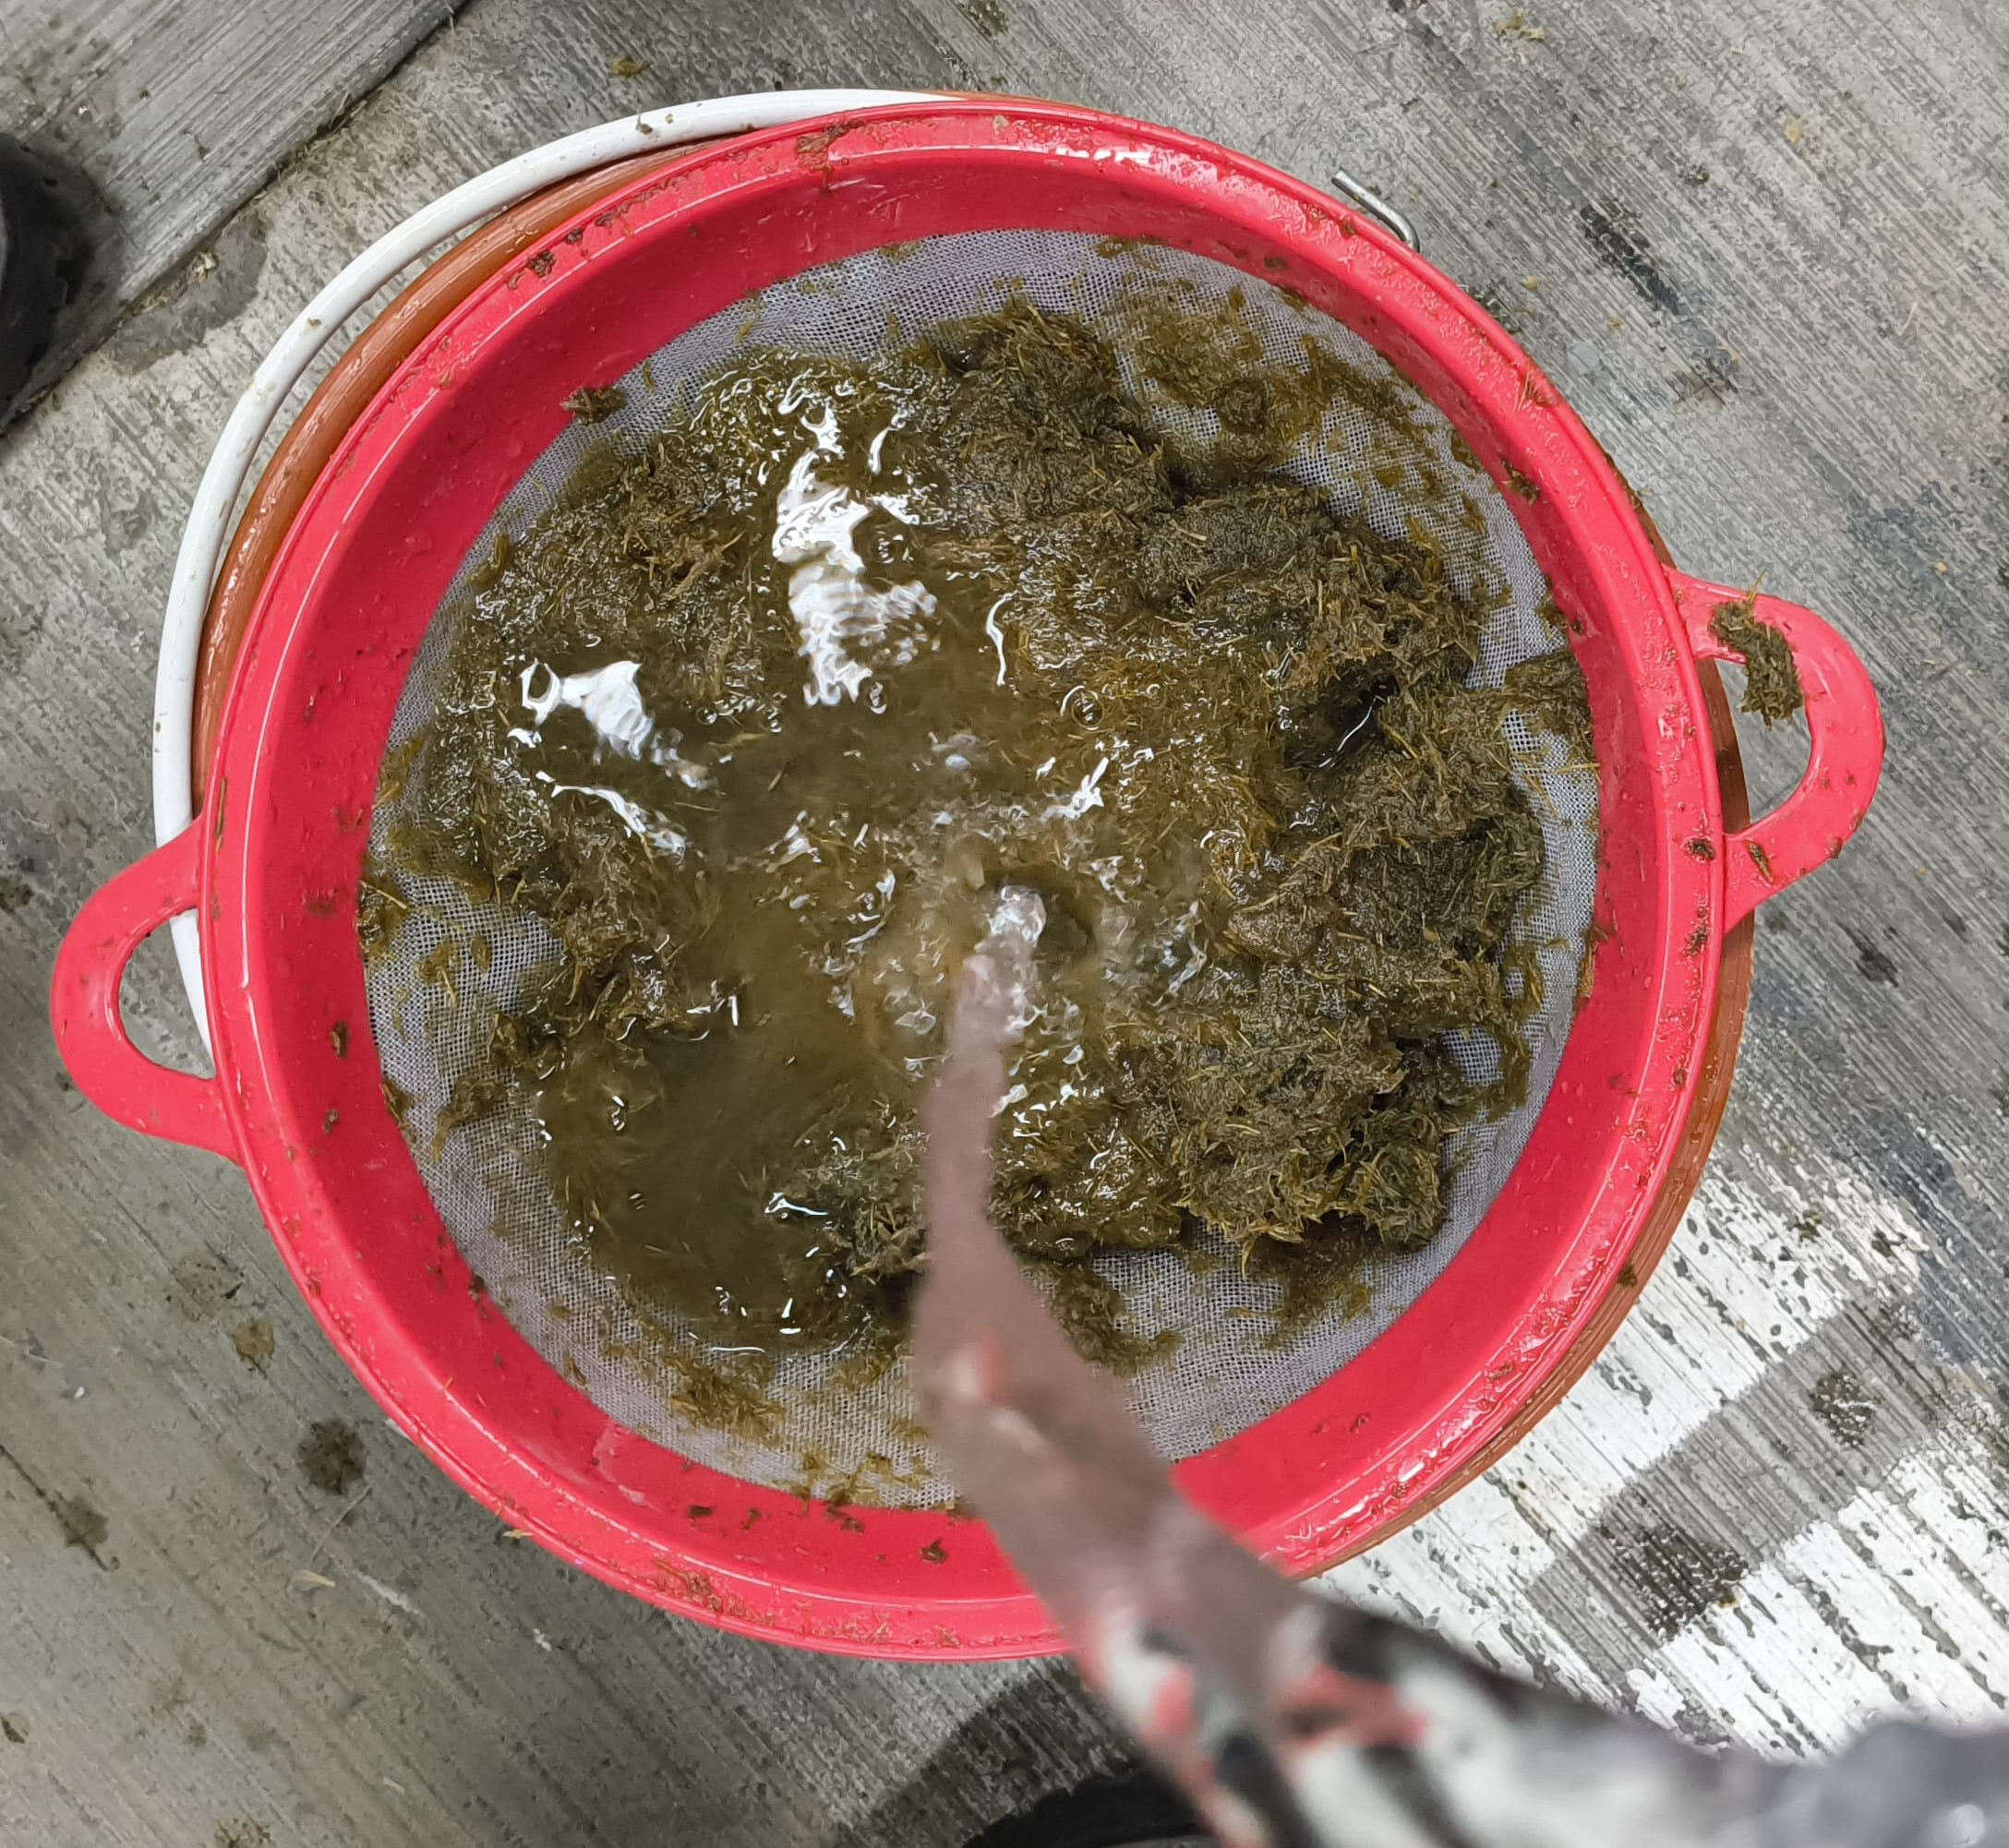
\includegraphics[width=5cm, height=3cm]{imagenes/enjuagado} % Cambia "imagen1.jpg" por el nombre de tu archivo
			\caption{En la fotografía muestra el bagazo después de filtrar el agua.}
			\label{enjuagado}
		\end{minipage}
		\hfill
		\begin{minipage}{0.48\textwidth}
			\centering
			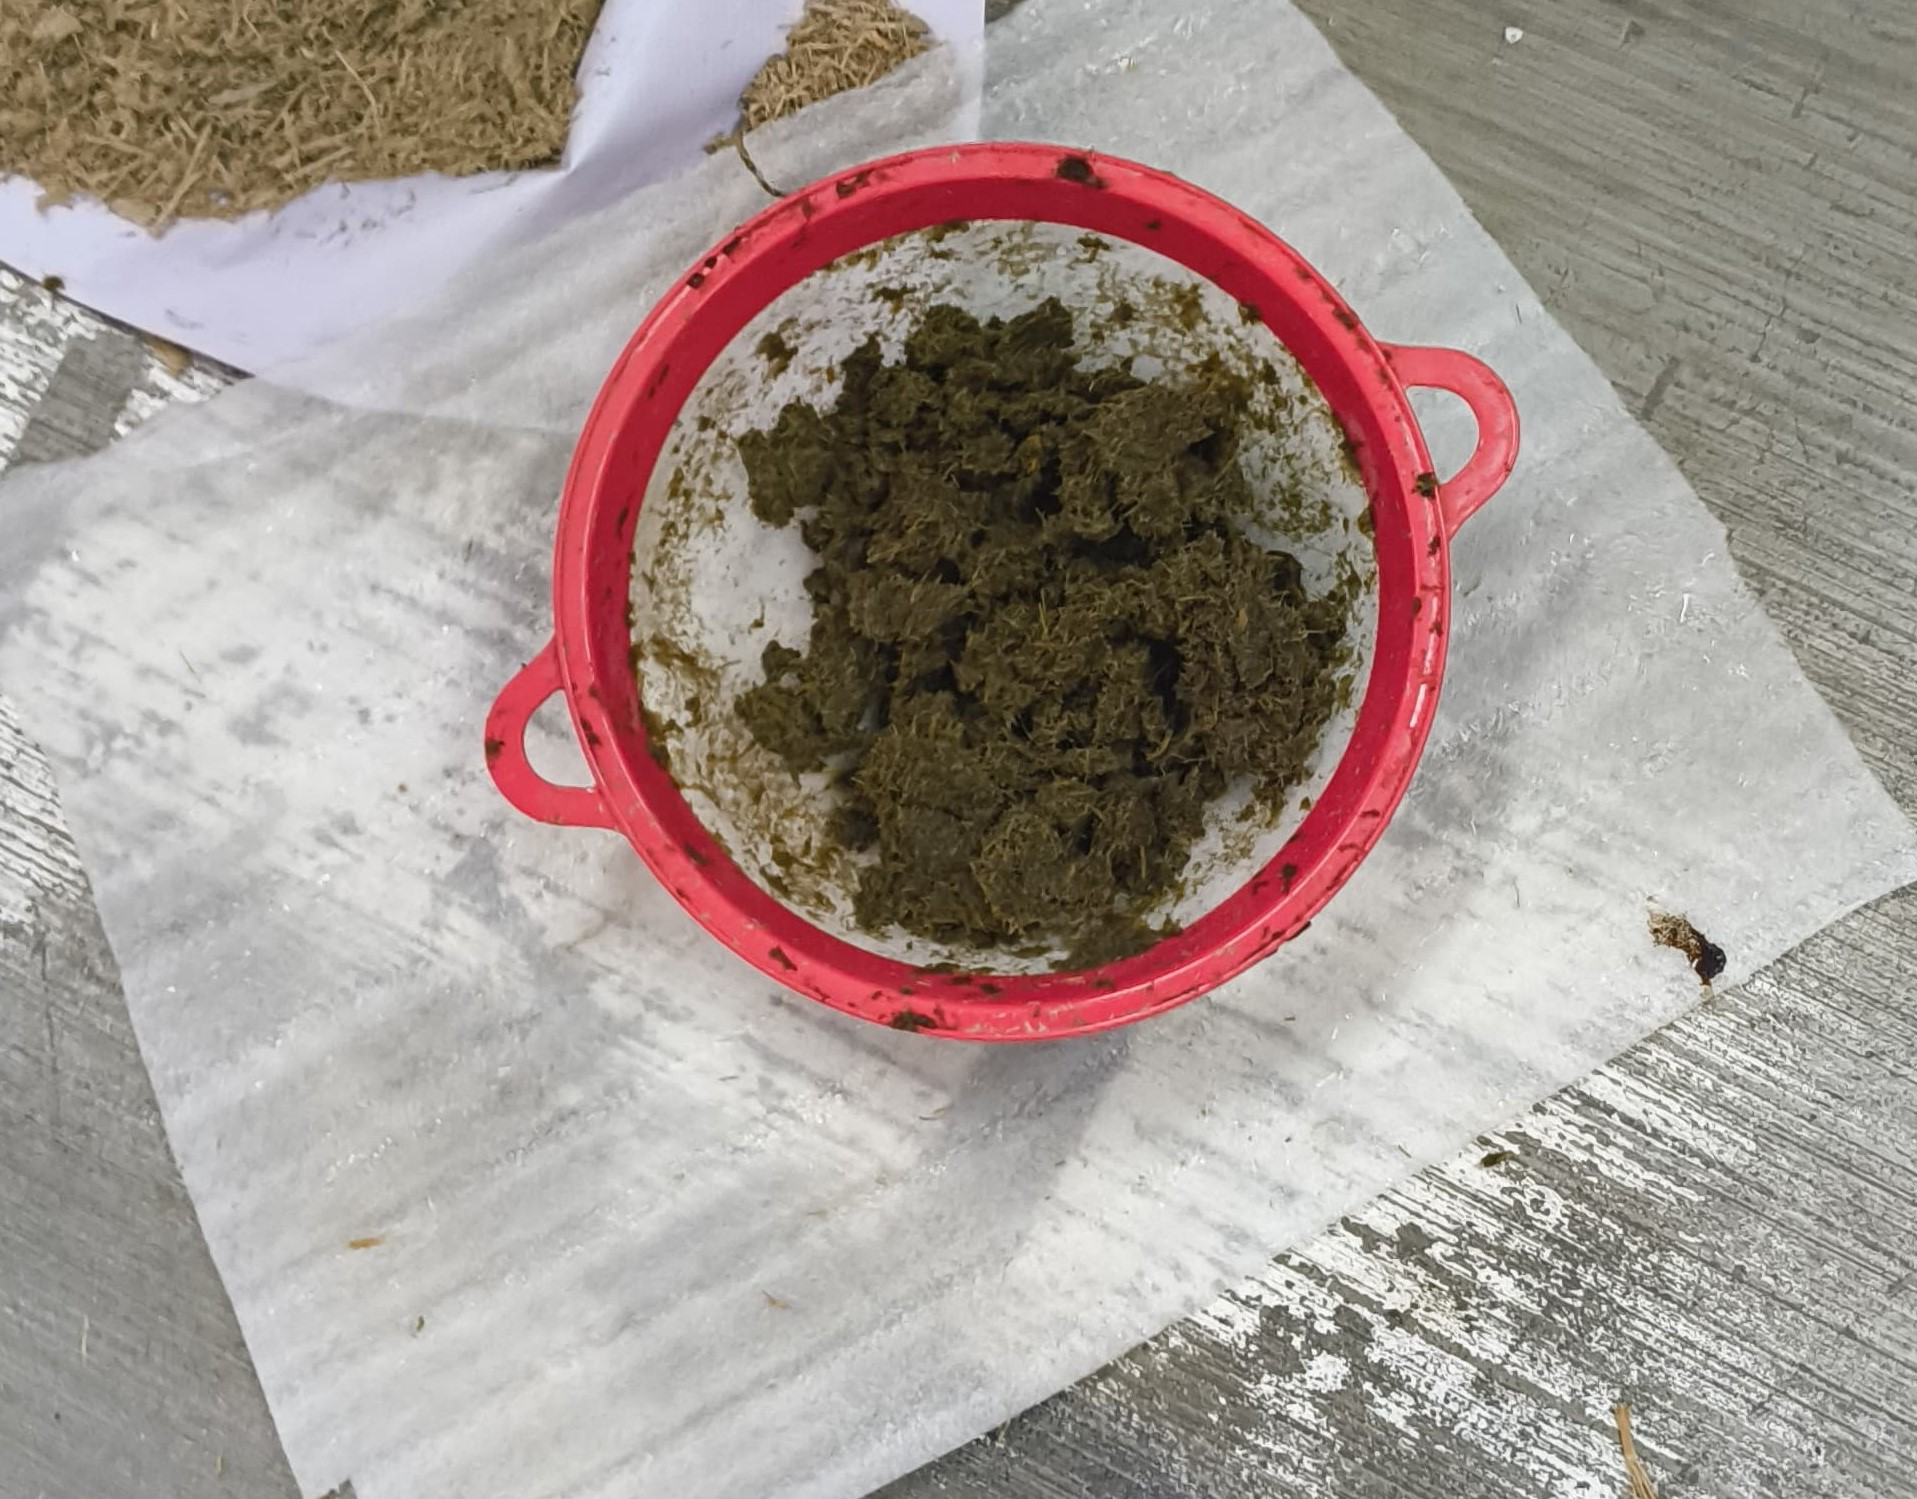
\includegraphics[width=4cm, height=3cm]{imagenes/secado6} % Cambia "imagen2.jpg" por el nombre de tu archivo
			\caption{El bagazo se coloca en un plástico para retirar el agua y la humedad.}
			\label{biologico4}
		\end{minipage}
	\end{figure}
	
	
	
	
	
	 \textbf{8.} Una vez completado el secado, el bagazo se almacena en bolsas herméticas para prevenir la absorción de humedad ambiental, garantizando así las condiciones óptimas para su uso en los posteriores procesos de hidrólisis y fermentación, tal como se muestra en la Figura \ref{biologico4}. Posteriormente el reactor tipo batch es lavado con agua desmineralizada. \\[0.5em]
	
	\textbf{9.} En el anexo \ref{diseño del control de temp} podemos observar el diseño del control de temperatura.
	

			
				\subsubsection{Hidrólisis y fermentación}
				
			Para la hidrólisis y fermentación se consideraron los datos del apartado del diseño factorial, a continuación se presenta la lista de materiales.
			\\
					 \textbf{Compuestos} \\[0.5em]
					 
				\begin{tabular}{p{0.3\textwidth}p{0.3\textwidth}p{0.3\textwidth}}	 
					 	 	$\bullet$ \textit{Agua desmineralizada} & $\bullet$ \textit{Enzimas Cellic Ctec 2}  & $\bullet$ \textit{Levadura activa} \\
					 $\bullet$ \textit{Ácido Cítrico} & $\bullet$ \textit{Bagazo de caña Pretratado} & \\
					
					\end{tabular}
					 
					 
					 	\textbf{Materiales} 
					 
					 \begin{tabular}{p{0.3\textwidth}p{0.3\textwidth}p{0.3\textwidth}}
					 $\bullet$ \textit{Cinta de teflón} & $\bullet$ \textit{Algodón } & $\bullet$ \textit{ Papel aluminio} \\
					 	$\bullet$ \textit{Cinta térmica}  & $\bullet$ \textit{Vaso de precipitado} &
					 \end{tabular}
					 \\[0.5em]
					 
					 
					 
		  \textbf{Procedimiento}
					\\[0.5em]	 
		 \textbf{1.}  El reactor tipo batch, previamente lavado, se desinfecta con agua desmineralizada y se procede a sellar herméticamente su base para garantizar condiciones estériles antes de iniciar el proceso, evitando así cualquier contaminación externa que pueda afectar la reacción.\\[0.5em]

		 	
		 \textbf{2.} Cada reactivo (ácido cítrico, levadura activa) se pesa individualmente usando una báscula calibrada y un vaso de precipitado estéril, mientras que el agua se mide volumétricamente, ajustando las cantidades según los parámetros establecidos en el diseño de experimentos para garantizar la reproducibilidad del proceso y la trazabilidad de los datos. Ver Figura\ref{pesado2}.
		 
	
		 
		 \begin{figure}[H]
		 	\centering
		 	\begin{minipage}{0.46\textwidth}
		 		\centering
		 		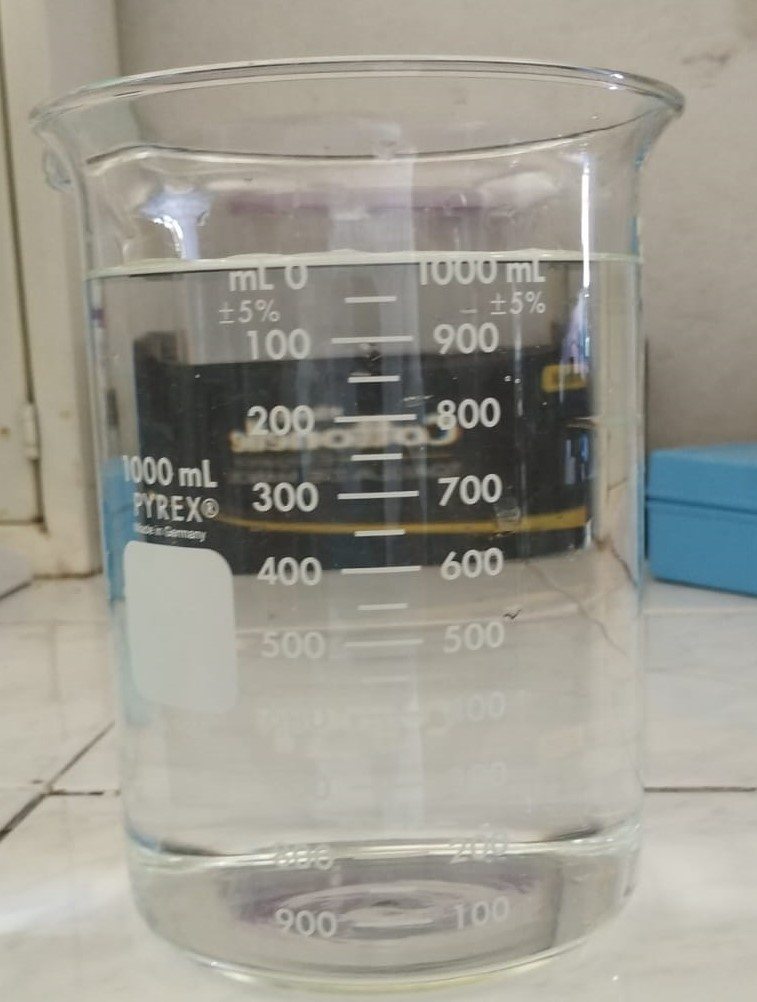
\includegraphics[width=3cm, height=3cm]{imagenes/agua} % Cambia "imagen1.jpg" por el nombre de tu archivo
		 		\caption{ Agua desmineralizada que ayudara a limpiar el reactor.}
		 		\label{agua}
		 	\end{minipage}
		 	\hfill
		 	\begin{minipage}{0.48\textwidth}
		 		\centering
		 		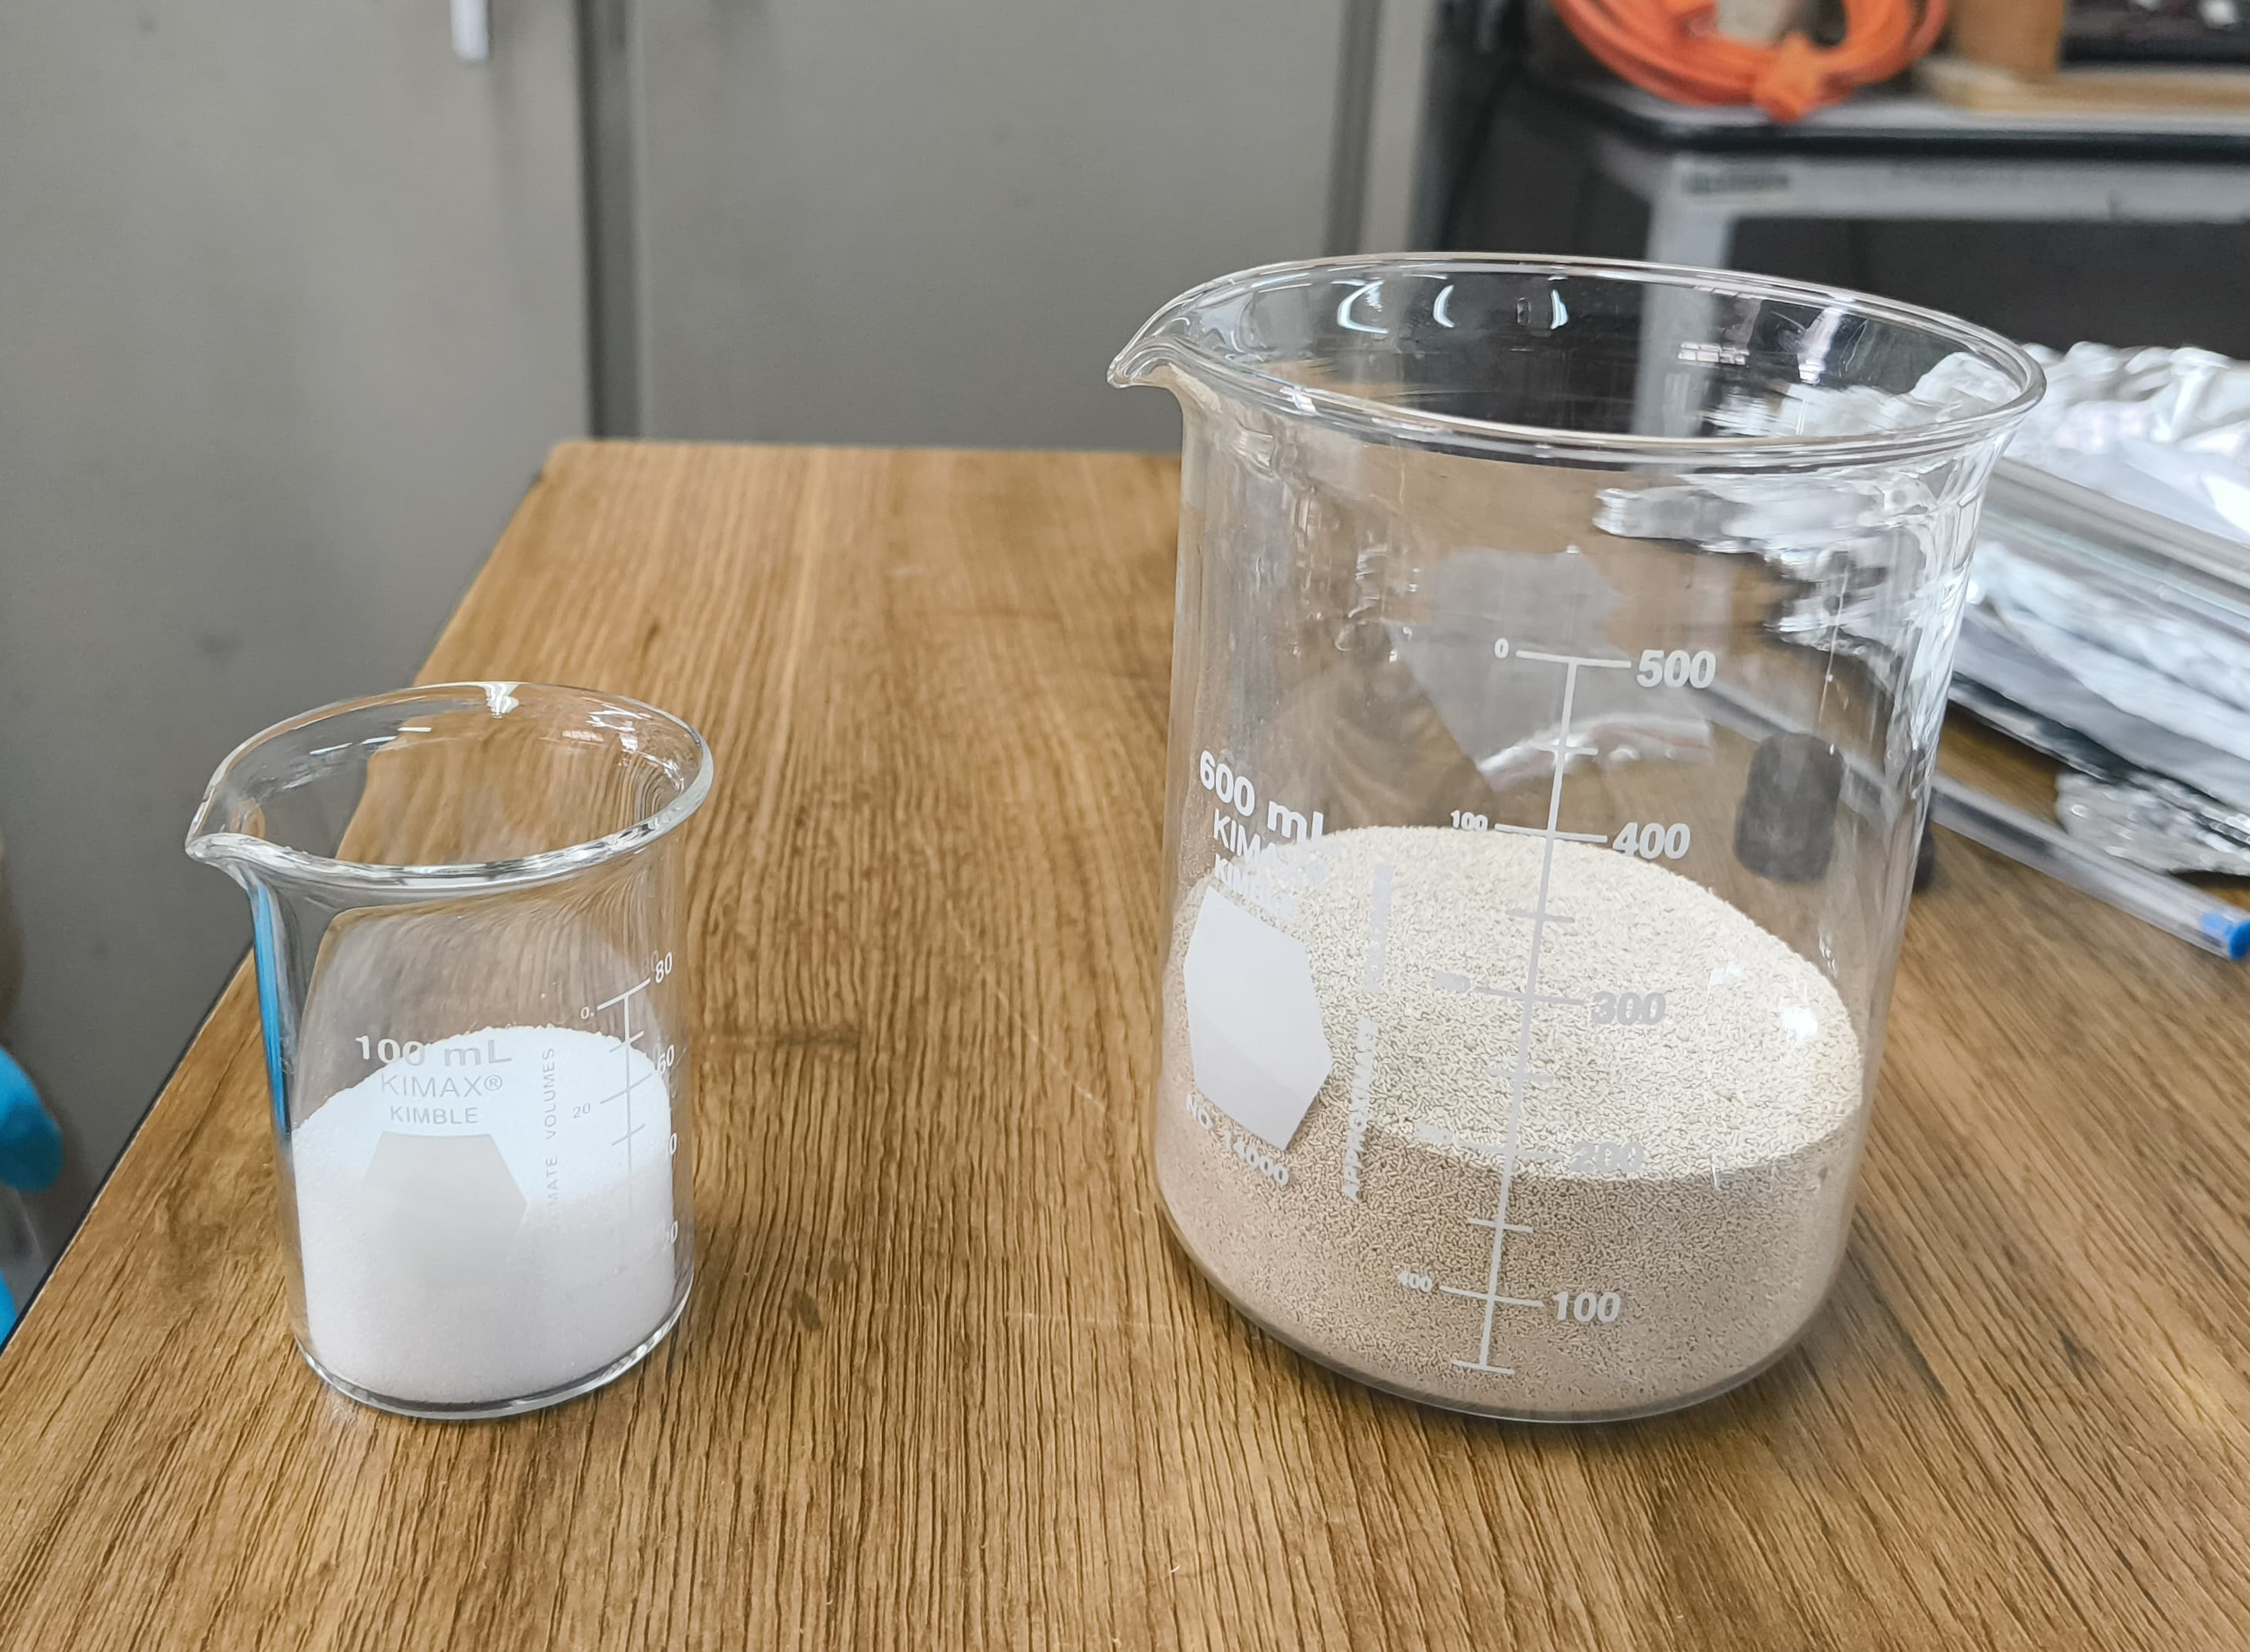
\includegraphics[width=4cm, height=3cm]{imagenes/levadura y acido citrico} % Cambia "imagen2.jpg" por el nombre de tu archivo
		 		\caption{Levadura y ácido cítrico}
		 		\label{pesado2}
		 	\end{minipage}
		 \end{figure}
		 
		 
	     \textbf{3.} En el interior del reactor tipo batch se depositan el agua desmineralizada y el bagazo de caña previamente pretratado, siguiendo las proporciones establecidas en el protocolo experimental (como se ilustra en la Figura \ref{ hidrolisis}), asegurando una distribución homogénea de los componentes para garantizar las condiciones óptimas de reacción.
	     	
	     \textbf{4.} Al reactor tipo batch que contiene el bagazo de caña pretratado y el agua desmineralizada se le adiciona la levadura activa previamente pesada (ver Figura \ref{hidrolisis4}), la cual se mezcla homogéneamente hasta lograr su completa incorporación al medio de reacción. 
	     
	    
	     
	      
	     \begin{figure}[H]
	     	\centering
	     	\begin{minipage}{0.46\textwidth}
	     		\centering
	     		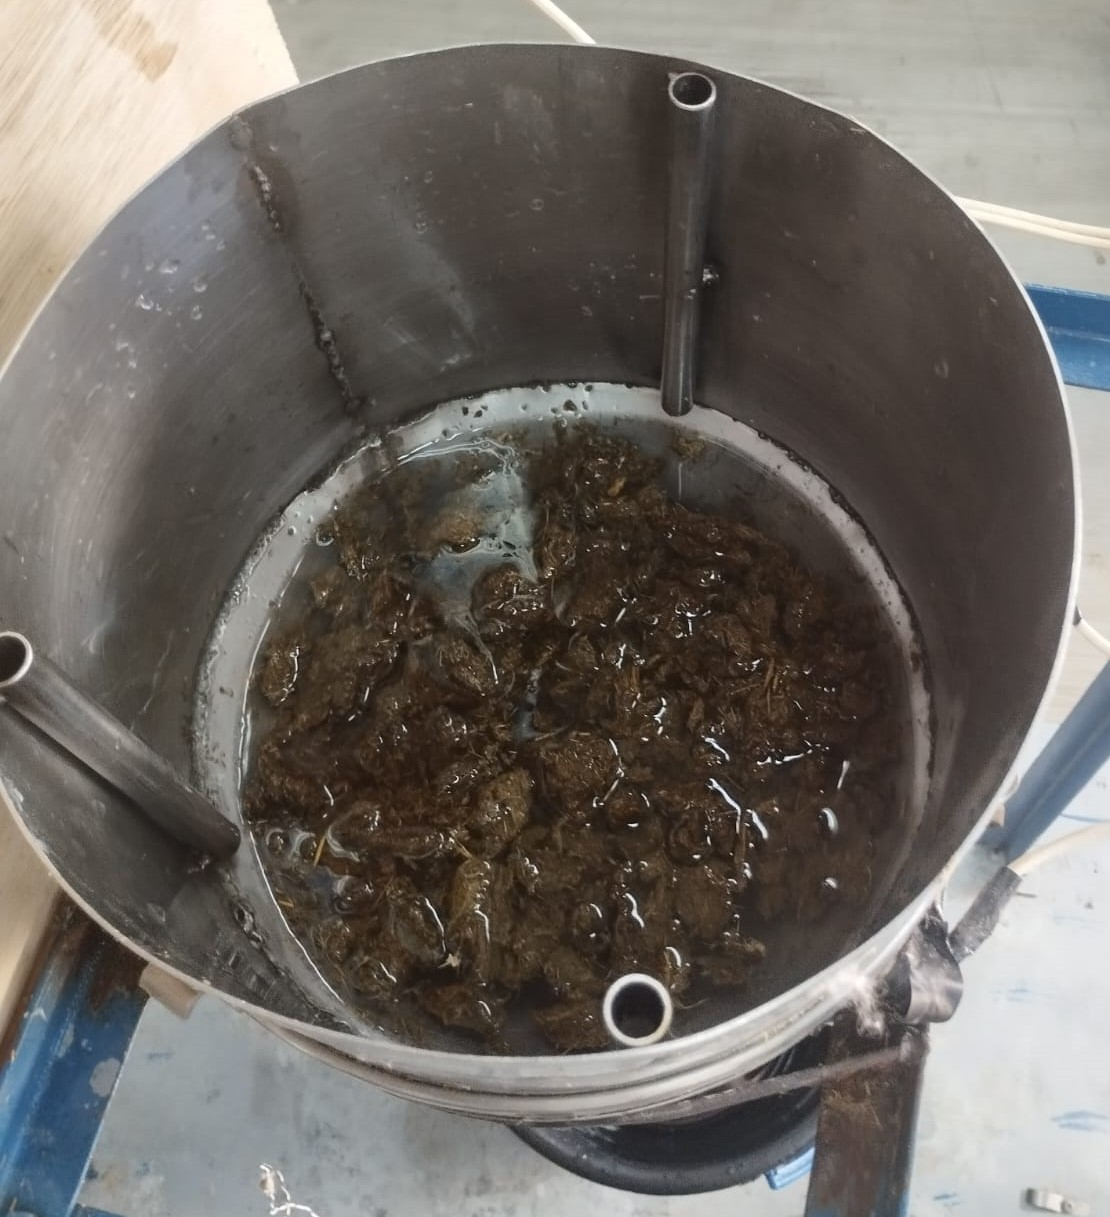
\includegraphics[width=3cm, height=3cm]{imagenes/hidrolisis1} % Cambia "imagen1.jpg" por el nombre de tu archivo
	     		\caption{ Reactor con bagazo previamente pretratado.}
	     		\label{ hidrolisis}
	     	\end{minipage}
	     	\hfill
	     	\begin{minipage}{0.48\textwidth}
	     		\centering
	     		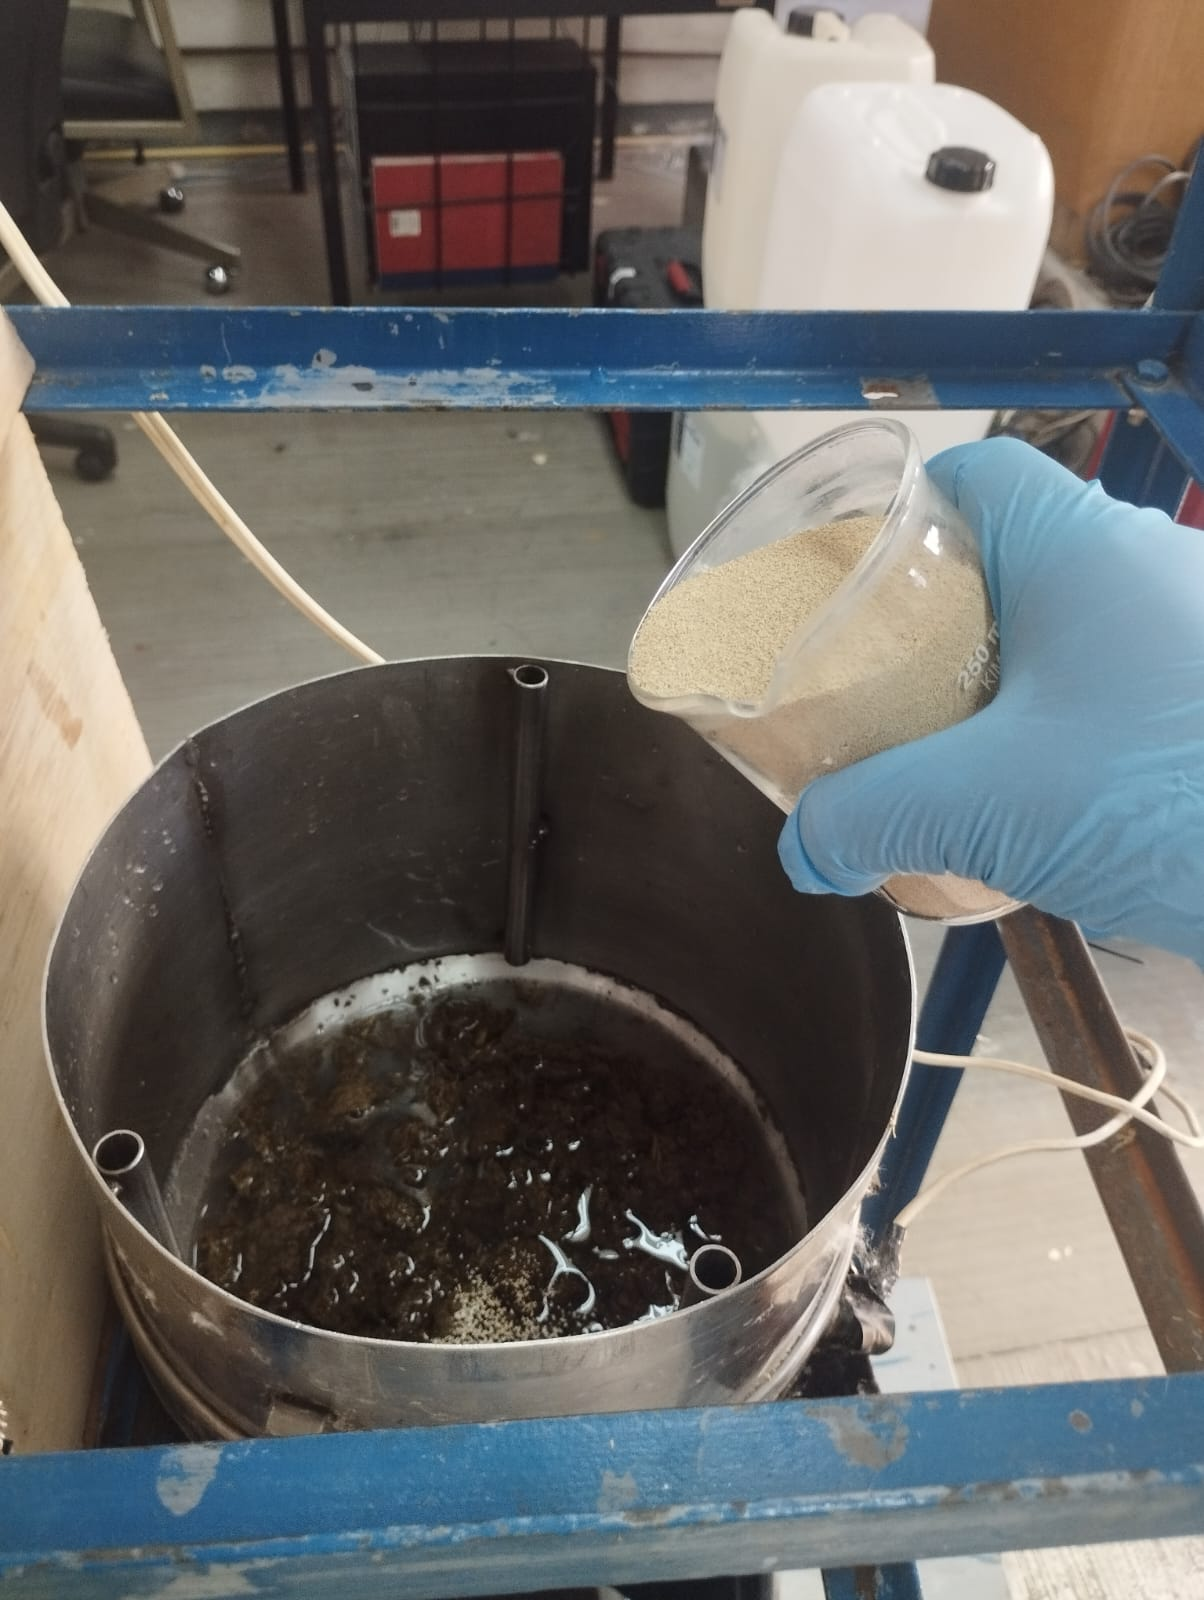
\includegraphics[width=4cm, height=3cm]{imagenes/hidrolisis4 } % Cambia "imagen2.jpg" por el nombre de tu archivo
	     		\caption{La levadura se agrega al reactor.}
	     		\label{hidrolisis4}
	     	\end{minipage}
	     \end{figure}
	     
	     
	     \textbf{5.} Mediante micropipeta calibrada se miden los mililitros exactos de la enzima Cellic CTec2 según el diseño de experimentos, la cual se añade al sistema y se mezcla meticulosamente hasta su completa integración (Figura \ref{hidrolisis9}), asegurando la actividad enzimática óptima	\\ 
	     	
	     	 
	     \textbf{6.} El pH de la mezcla se mide utilizando un medidor de pH Hanna Instruments previamente calibrado, introduciendo el electrodo en la solución y agitando suavemente para obtener una lectura estable; dependiendo del resultado, se añade gradualmente ácido cítrico en cantidades pesadas con precisión, monitoreando el cambio en el pH después de cada adición hasta alcanzar el valor deseado según los parámetros establecidos en el diseño experimental, ver figura \ref{hidrolisis3}.
	     
	     
	     
	     \begin{figure}[H]
	     	\centering
	     	\begin{minipage}{0.46\textwidth}
	     		\centering
	     		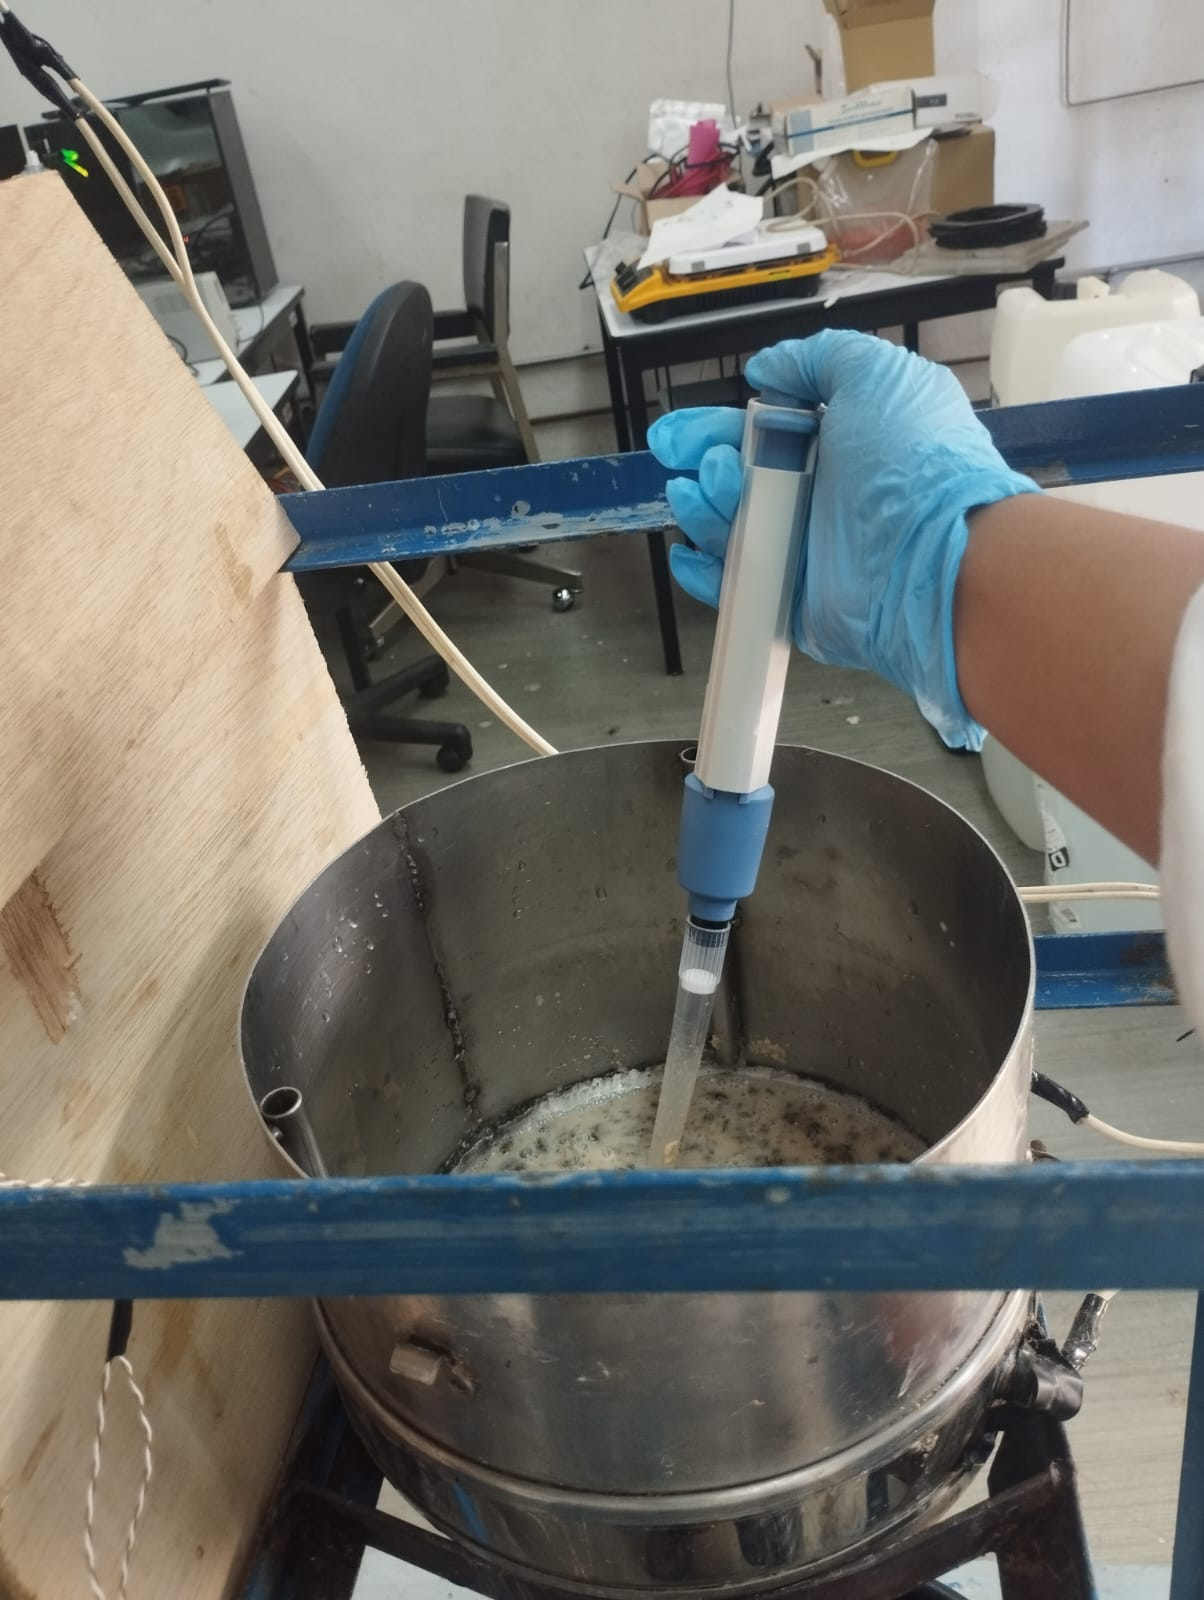
\includegraphics[width=5cm, height=3cm]{imagenes/hidrolisis9} % Cambia "imagen1.jpg" por el nombre de tu archivo
	     		\caption{ Se agrega la enzima al reactor con ayuda de la micropipeta }
	     		\label{hidrolisis9}
	     	\end{minipage}
	     	\hfill
	     	\begin{minipage}{0.48\textwidth}
	     		\centering
	     		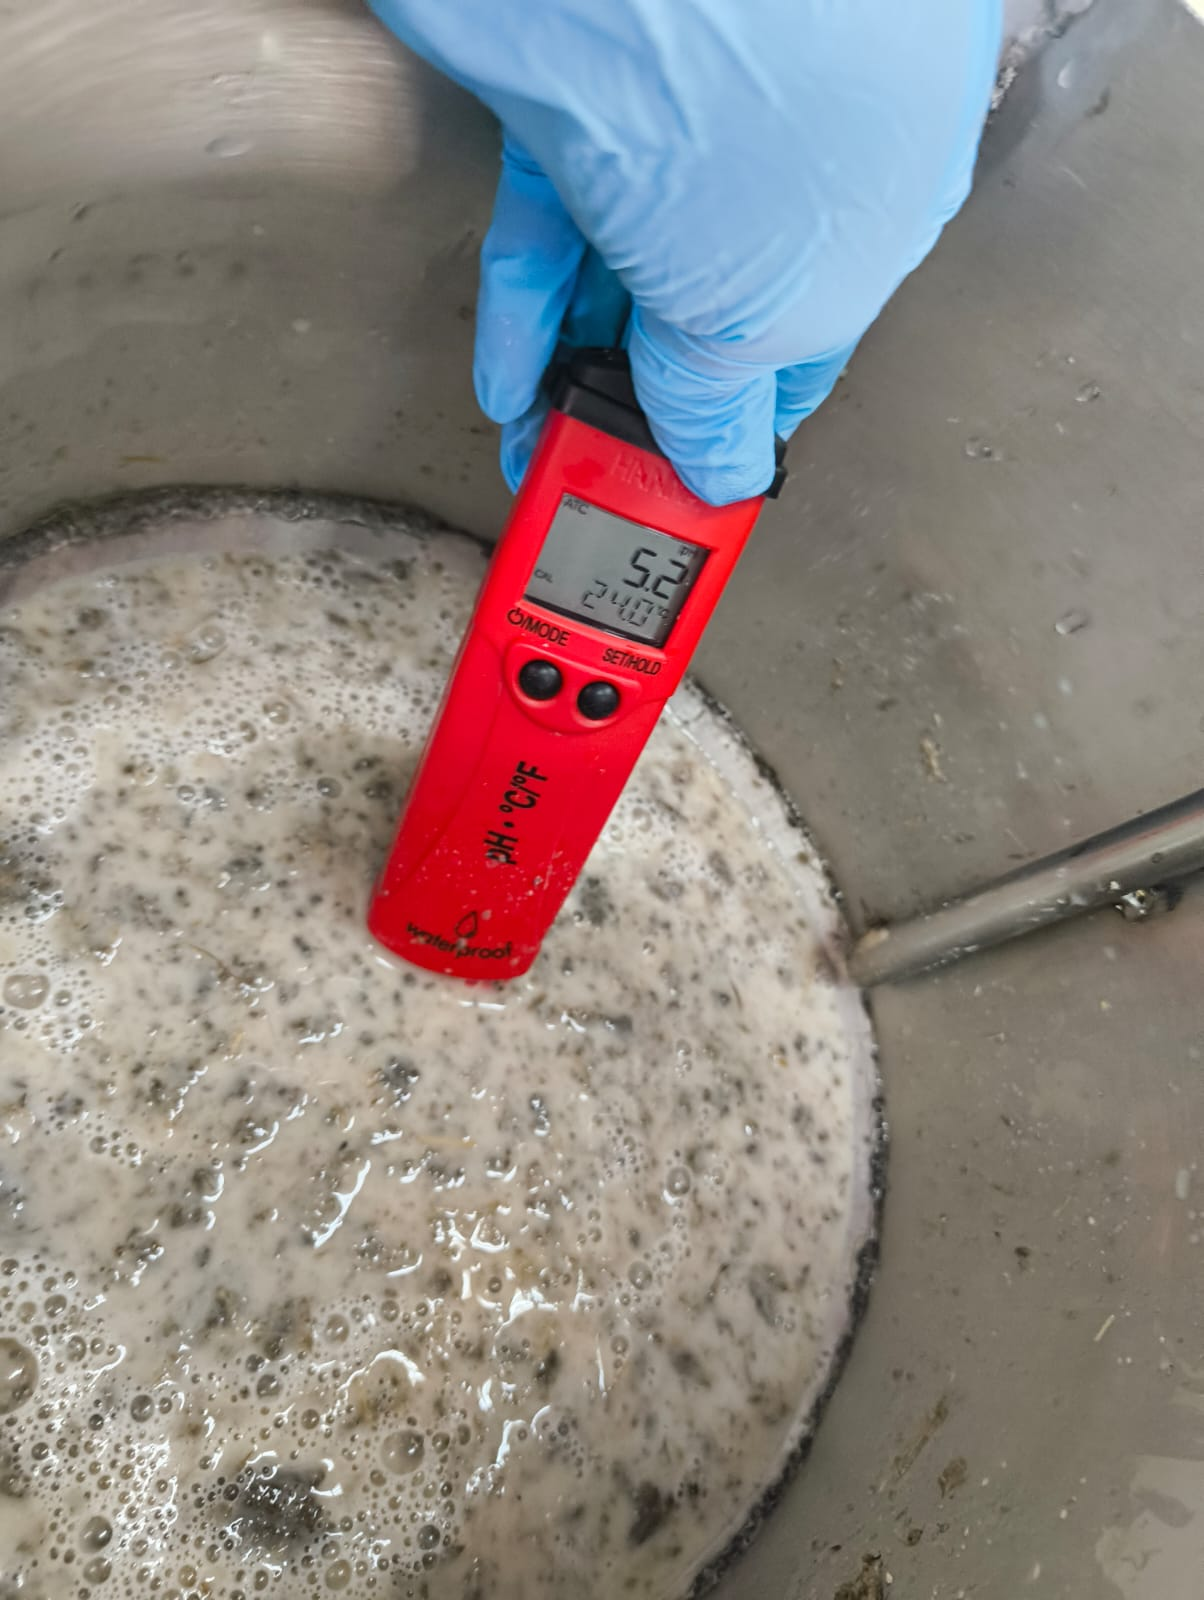
\includegraphics[width=5cm, height=3cm]{imagenes/hidrolisis3 } % Cambia "imagen2.jpg" por el nombre de tu archivo
	     		\caption{ Se mide el ph de la mezcla con ayuda del medidor hanna instruments.}
	     		\label{hidrolisis3}
	     	\end{minipage}
	     \end{figure}
	     
	      \textbf{7.} El reactor tipo batch se sella herméticamente utilizando algodón y papel aluminio (ver Figura \ref{hidrolisis 6}), y se instala una trampa de aire compuesta por una manguera insertada en uno de los orificios de la tapa del reactor tipo batch. Para garantizar un cierre seguro y evitar fugas, se refuerza la conexión entre la manguera y la tapa con cinta adhesiva. El extremo libre de la manguera se sumerge en una cubeta con agua, permitiendo la liberación controlada del dióxido de carbono generado durante la reacción, al mismo tiempo que impide la entrada de oxígeno al sistema. Este diseño asegura un ambiente anaeróbico adecuado para el proceso.
	      \\[0.5em]
	     
	     	\textbf{8.} Se inicia el sistema de control para la hidrólisis y fermentación, ajustando los parámetros de tiempo y temperatura según las condiciones predefinidas en el diseño experimental (ver apartado \ref{SacariSF}), garantizando así las condiciones óptimas para el proceso. Ver Figura \ref{hidrolisis 8} para observar la estructura y conexiones.
	     	
	 
	     		     \begin{figure}[H]
	     		\centering
	     		\begin{minipage}{0.46\textwidth}
	     			\centering
	     			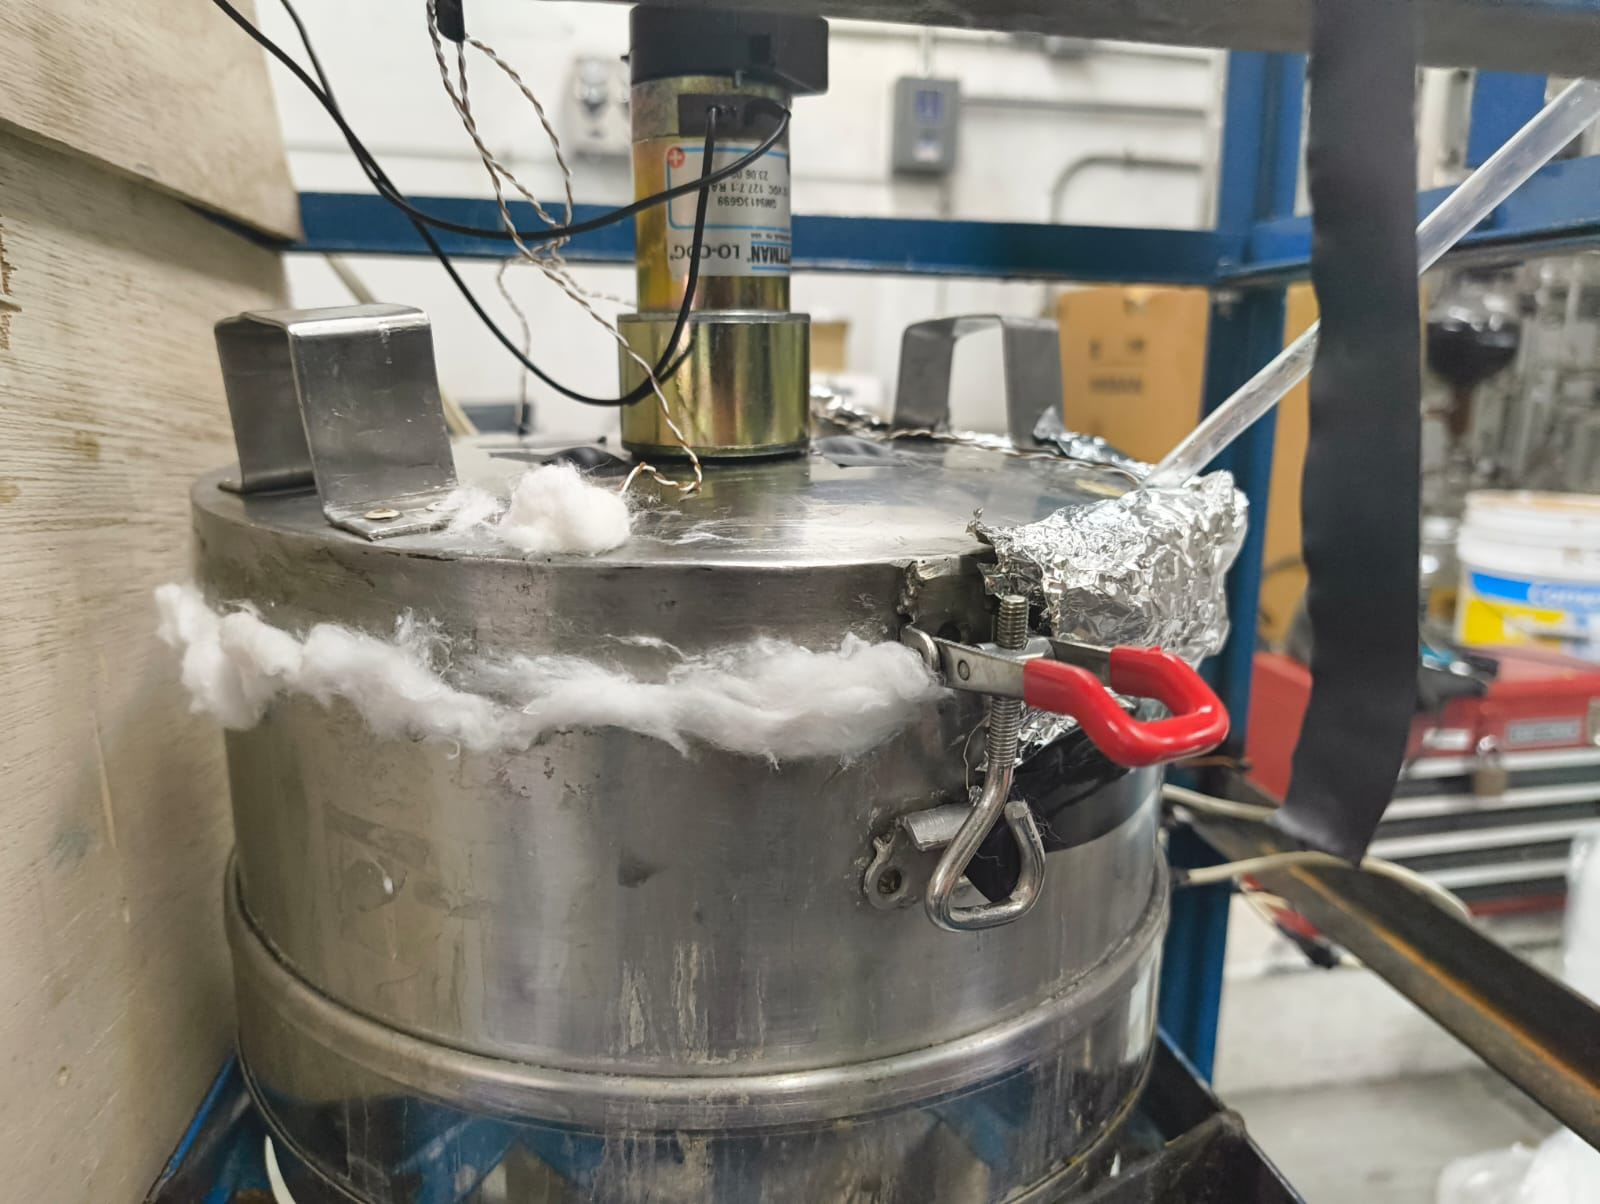
\includegraphics[width=5cm, height=3cm]{imagenes/hidrolisis 6} % Cambia "imagen1.jpg" por el nombre de tu archivo
	     			\caption{ El algodón es colocado entre la tapa para tratar de que el reactor sea lo mas hermético posible }
	     			\label{hidrolisis  6}
	     		\end{minipage}
	     		\hfill
	     		\begin{minipage}{0.48\textwidth}
	     			\centering
	     			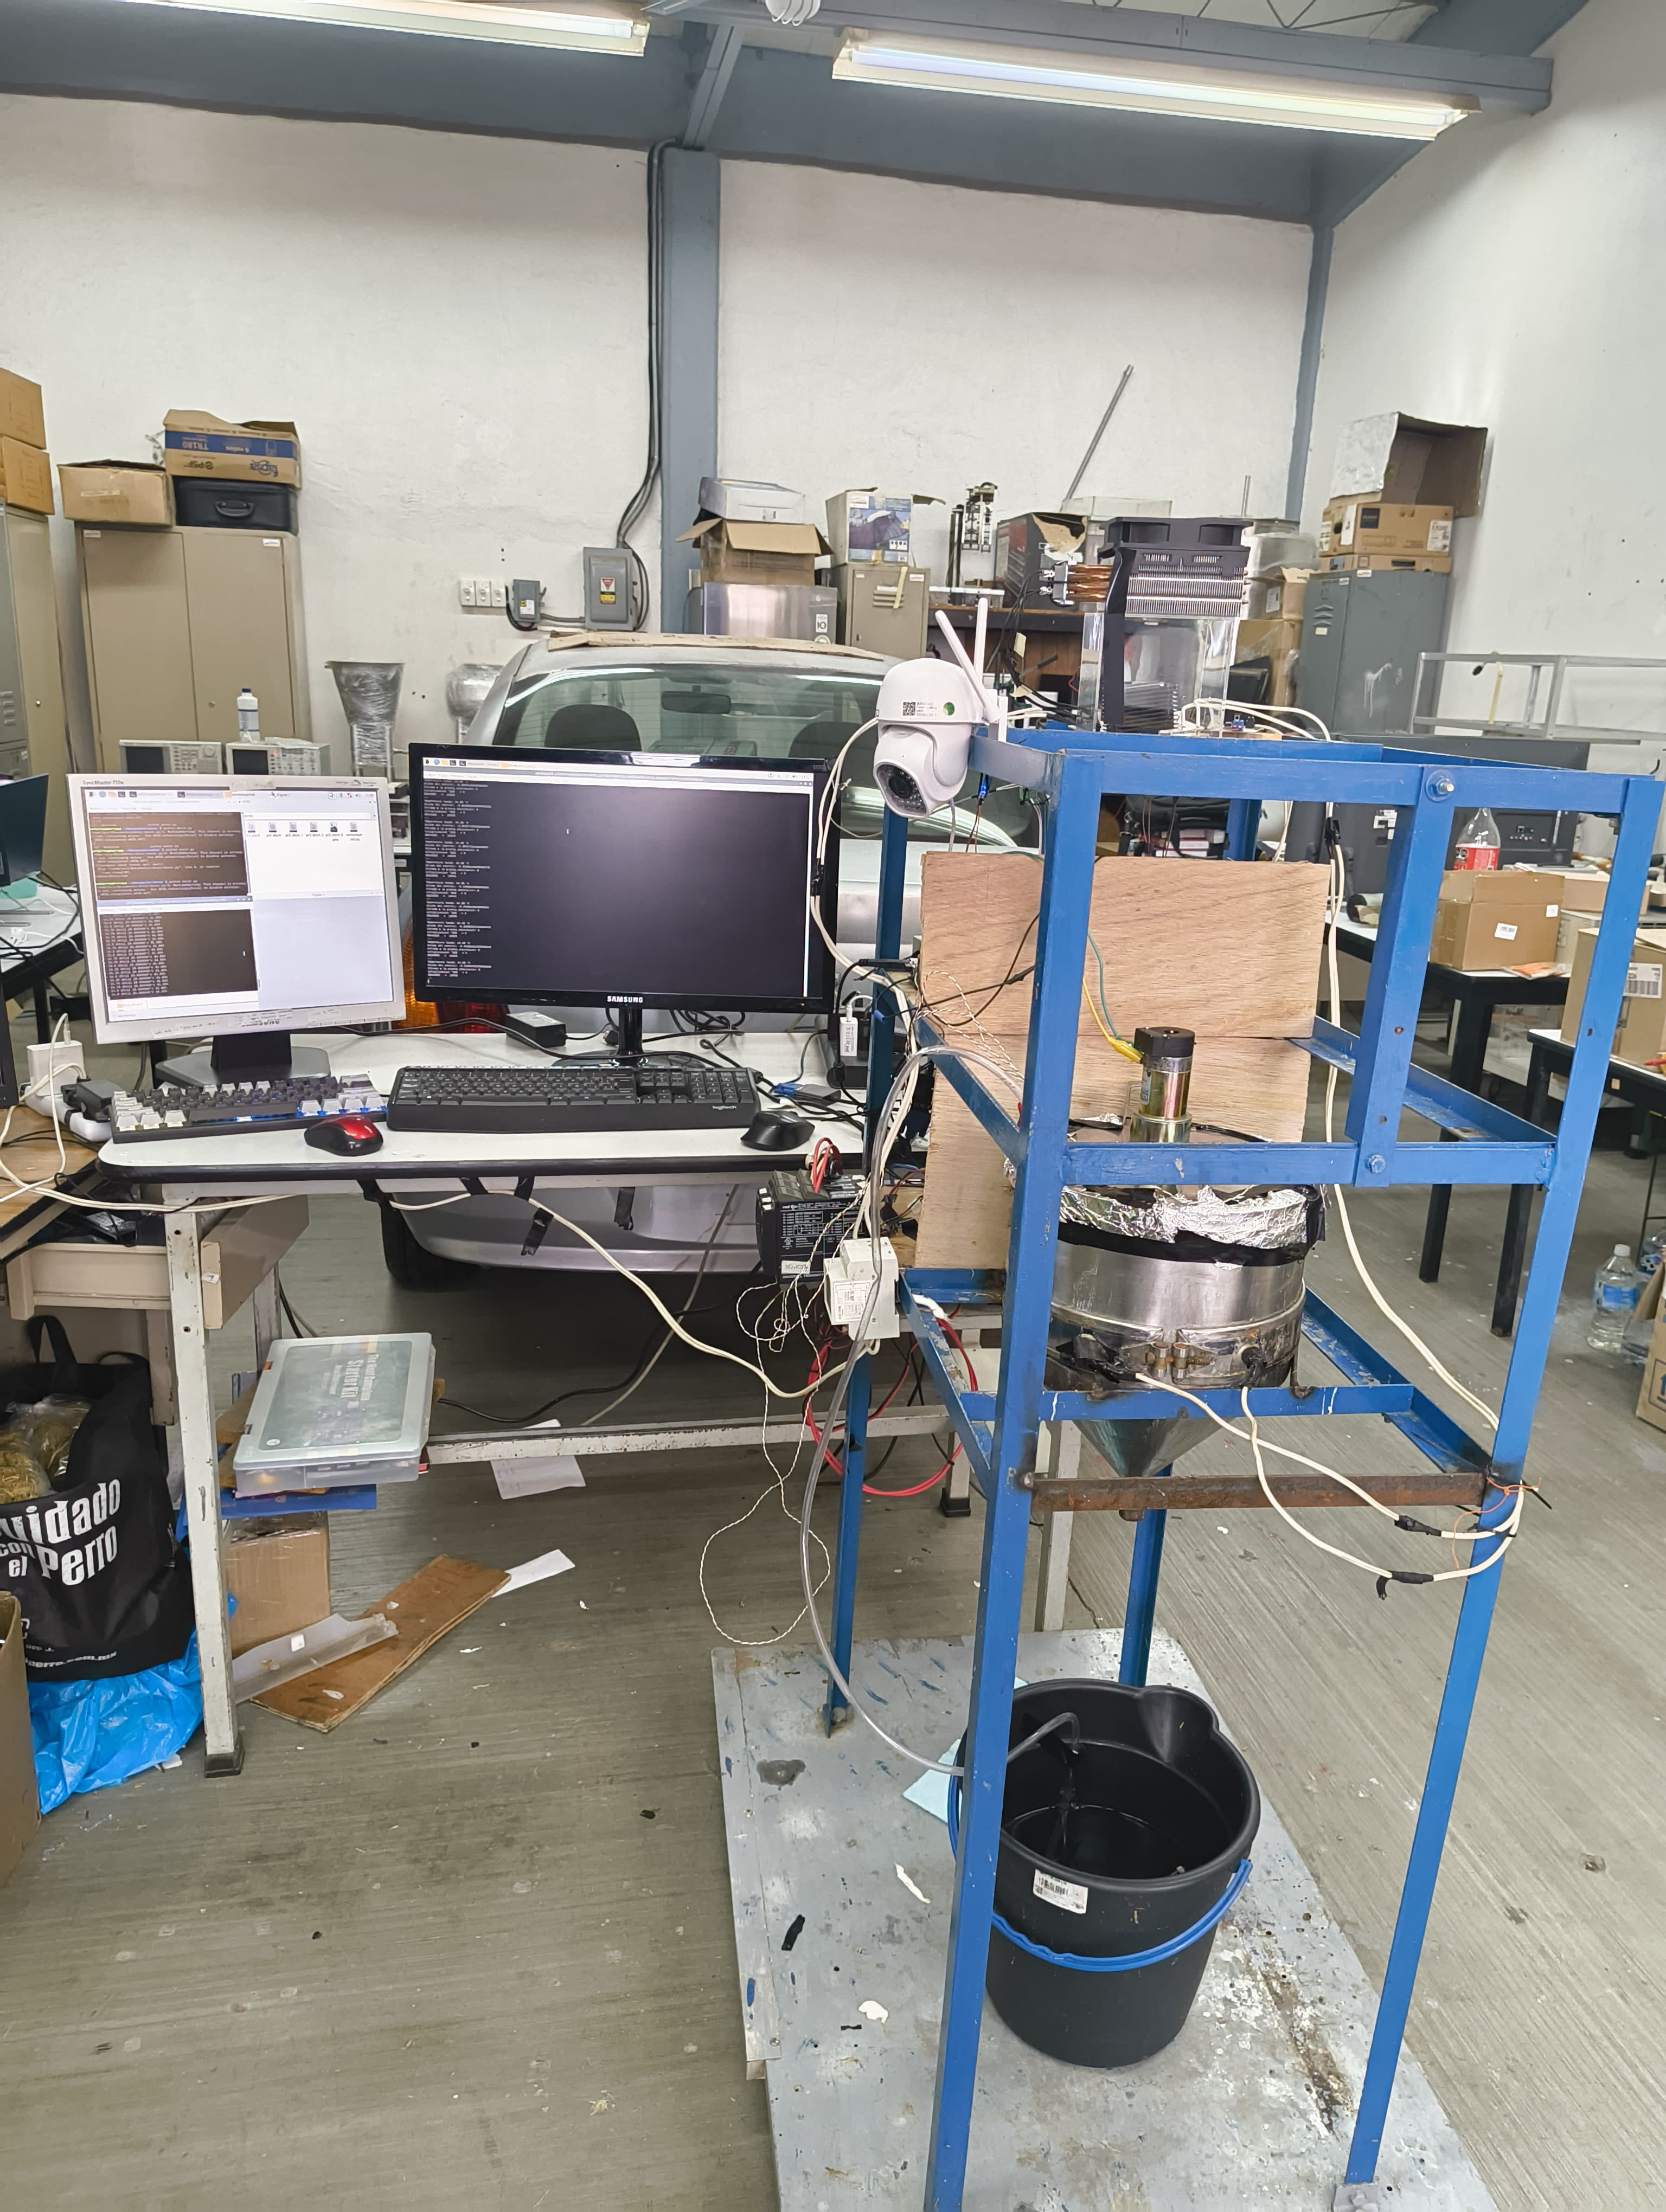
\includegraphics[width=3cm, height=3cm]{imagenes/conexion de hidrolisis } % Cambia "imagen2.jpg" por el nombre de tu archivo
	     			\caption{ Puesta en marcha del control en la etapa de hidrólisis y fermentación en un reactor tipo batch}
	     			\label{hidrolisis 8}
	     		\end{minipage}
	     	\end{figure}
	     	
	     	
	     	\textbf{9.} Finalizado el proceso de hidrólisis y fermentación, se determina el pH final del producto (Figura \ref{hidrolisis 7}) y se transfiere a recipientes herméticos, los cuales se almacenan a temperaturas inferiores a 30°C para preservar las muestras hasta la cuantificación del contenido alcohólico. Finalmente el reactor tipo batch es lavado con agua desmineralizada.
	     	
	     	
	     		   	\begin{figure}[H]
	     		\centering
	     		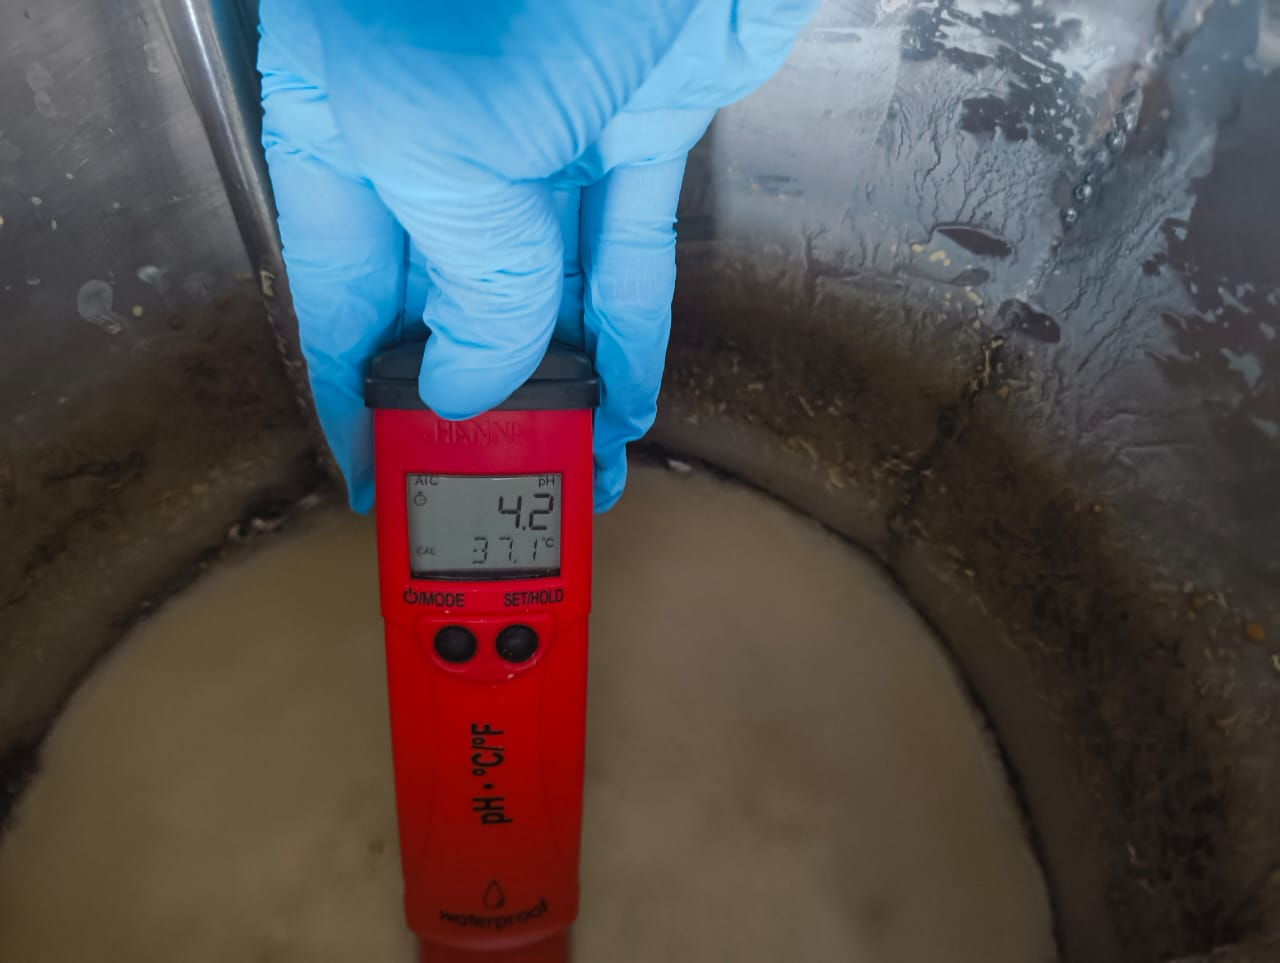
\includegraphics[width=5cm, height=3cm]{imagenes/hidrolisis7}
	     		\caption{ Medición del ph de la mezcla después de la hidrólisis y fermentación}
	     		\label{hidrolisis 7}
	     	\end{figure}
	     	
	     	
	     	\textbf{10.} Se puede observar el diseño del control en el anexo \ref{diseño del control de temp}.
	     	
	     	
			%%%%%%%%%%%%%%%%%%%%%%%%%%%%%%%%%%%%%%%%%%%%%%%%%%%%%%%%%%%%%%%%%%%%%
			
			
			%%%%%%%%%%%%%%%%%%%%%%%%%%%%%%%%%%%%%%%%%%%%%%%%%%%%%%%%%%%%%%%%%%%%%%%%%%%%%%%%%%%%%%%%%%%%%%%%%%%%%%%%%%%%%%%%%%%%%%%%%%%%%%%%%%%%%%%%%%%%%%%%%%%%%%%%%%%%%%%%%%%%%%%%%%%%%%%%%%%%%%%%%%%%%%%%%%%%%%%%%%%%%%%%%%%%%%%%%%%%%%%%%%%%%%%%%%%%%%%%%%%%%%%%%%%%%%%%%%%%%%%%%%%%%%%%%%%%%%%%%%%%%%%%%%%%%%%%%%%%%%%%%%%%%%%%%%%%%%%%%%%%%%%%%%%%%%%%%%%%%%%%%%%%%%%%%%%%%%%%%%%%%%%%%%%%%%%%%%%%%%%%%%%%%%%%%%%%%%%%%%%%%%%%%%%%%%%%%%%%%%%%%%%%%%%%%%%%%%%%%%%%%%%%%%%%%%%%%%%%%%%%%%%%%%%%%%%%%%%%
		

				\subsection{Resultados experimentales del proceso de producción de bioetanol 2 G con pretratamiento Alcalino  y Biológico}
				Siguiendo el proceso para la producción de bioetanol de segunda generación se realizo un pretratamiento y posteriormente una hidrólisis y fermentación en una misma etapa, los resultados obtenidos se clasificaron con base a el diseño de experimentos del apartado \ref{Diseño factorial del pretratamiento alcalino}.
				
				
				
		
		\subsubsection{Pretratamiento Biológico}
	Los pretratamientos biológicos realizados sobre bagazo de caña de azúcar (Tabla \ref{Pretratamiento Biológico}) comprendieron tres pruebas con granulometría de tamaño no uniforme de bagazo (1 mm - 10 cm) y tres pruebas con granulometría constante (1 cm) bajo temperaturas controladas (30, 40 y 45 °C), registrándose el consumo energético (kWh) en cada caso. Como parte del proceso de producción de bioetanol,  Este diseño experimental permitió evaluar comparativamente las diferencias en los costos asociados al consumo energético. 
		
	\begin{table}[H]
		\centering
		\caption{Preubas experimentales con pretratamiento biológico}
		\begin{tabular}{|c|c|c|c|}
			\hline
			\textbf{Num de} &\textbf{ Temperatura} & \textbf{Tamaño de bagazo} & \textbf{Consumo energético } \\ 
			\textbf{de experimento} &\textbf{  (°c)} &  & \textbf{ (kwh)} \\ \hline
			1 & \multirow{2}{*}{45} & TNUB & 4.55 \\ \cline{1-1} \cline{3-4}
			2 &  & 1 cm & 3.81 \\ \hline
			3 &\multirow{2}{*}{ 40} & TNUB & 2.77 \\ \cline{3-4} \cline{1-1}
			4 &  & 1 cm & 2.81 \\ \hline
			5 &\multirow{2}{*}{ 30} & TNUB & 4.55 \\ \cline{3-4}\cline{1-1}
			6 &  & 1 cm & 1.11 \\ \hline
		\end{tabular}
		\label{Pretratamiento Biológico}
	\end{table}
	
	Las pruebas anteriores se realizaron en un tiempo de 5 días
		%%%%%%%%%%%%%%%%%%%%%%%%%%%%%%%%%%%%%%%%%%%%%%%%%%%%%%%%%%%%%%%%%%%%%%%%%%%
		
		\subsubsection{Pretratamiento Alcalino}
		
		
		Ya que el tiempo de establecimiento del control dura menos se propuso modificar el tiempo como en las pruebas utilizando 1 cm de bagazo de caña por lo que a continuación se muestras las pruebas utilizando un tiempo de 7870 con bagazo de caña de 1 mm hasta 10 cm o tamaño no uniforme de bagazo(TNUB)) y 1 cm, llevándose a cabo 6 pruebas experimentales para ese tiempo y 6 pruebas para 1 cm de bagazo, como se puede observar en la Tabla \ref{Pretratamiento Alcalino}. 
		Se busco monitorear la energía consumida en cada una de las pruebas, por lo que la columna 10 muestra mediante kwh la energía que fue leída de un watimetro.
		
		
		\begin{table}[H]
			\centering
			\caption{Preubas experimentales con pretratamiento alcalino}
			\begin{tabular}{|c|c|c|c|c|}
				\hline
				\textbf{Num de} & \textbf{Temperatura} & \textbf{Tamaño de } & \textbf{Tiempo} & \textbf{Consumo } \\ 
			\textbf{de experimento}	&\textbf{ (°c)}&\textbf{ bagazo}  &\textbf{(s)}	&\textbf{ energético (kwh)}\\ \hline
				1 & \multirow{4}{*}{95} & \multirow{2}{*}{TNUB} & 5400 & 0.66  \\ \cline{1-1} \cline{4-5}
				2 &  &  & 7870 & 0.81  \\ \cline{3-5}  \cline{1-1} 
				3 &  & \multirow{2}{*}{1 cm} & 5400 & 0.74 \\  \cline{1-1} \cline{4-5}
				4 &  &  & 7870 & 0.86 \\ \cline{1-1}  \hline
				5 & \multirow{4}{*}{90}& \multirow{2}{*}{TNUB} & 5400 & 0.71  \\ \cline{1-1}  \cline{4-5}
				6 &  &  & 7870 & 0.7  \\ \cline{1-1} \cline{3-5}
				7 &  & \multirow{2}{*}{1 cm} & 5400 & 0.74 \\ \cline{1-1}\cline{4-5}
				8 &  &  & 7870 & 0.6 \\ \hline
				9 & \multirow{4}{*}{80} & \multirow{2}{*}{TNUB} & 5400 & 0.67  \\ \cline{1-1}\cline{4-5}
				10 &  &  & 7870 & 0.63  \\ \cline{1-1} \cline{3-5}
				11 &  &\multirow{2}{*}{1 cm} & 5400 & 0.78 \\ \cline{1-1}\cline{4-5}
				12 &  &  & 7870 & 0.8 \\ \hline
			\end{tabular}
			\label{Pretratamiento Alcalino}
		\end{table}
		
		
		
		
	
	%%%%%%%%%%%%%%%%%%%%%%%%%%%%%%%%%%%%%%%%%%%%%%%%%%%%%%%%%%%%%%%%%%%%%%%%%%%%%%%%%%%%%%%%%%%%%%%%%%%%%%%%%%%%%%%%%%%%
	\subsection{Resultados experimentales del proceso de producción de bioetanol en la etapa de hidrólisis y fermentación utilizando diferentes tipos de pretratamiento}
A continuación se presentan los resultados de las pruebas experimentales después de realizar la etapa de hidrólisis y fermentación en conjunto. Los datos a considerar son la cantidad de alcohol obtenida, así como el consumo energético en las etapas en conjunto.
			%%%%%%%%%%%%%%%%%%%%%%%%%%%%%%%%%%%%%%%%%%%%%%%%%%%%%%%%%%%%%%%%%%%%%%%%%%%%%%%%%%%%%%%%%%%%%%%%%%%%%%%%%%%%%%%%%%%%%%%%%%%%%%%%%%%%%%%%%%%%%%%%%%%%%%%%%%%%%%%%%%%%
   	\subsubsection{ Hidrólisis y fermentación para pretratamiento Biológico}
   
   Posteriormente según el proceso de producción de bioetanol se realiza una hidrólisis y fermentación en conjunto, para cada uno de los pretratamientos realizados en la Tabla \ref{ssf Pretratamiento Biológico} menciona las 6 pruebas realizadas a tres temperaturas diferentes con dos tamaños de partícula. Durante las pruebas se registraron la energía consumida, por lo que en la columna cuatro menciona el dato en kwh.

 	\begin{table}[H]
 		\centering
 		\caption{Hidrólisis y fermentación con pretratamiento biológico}
 		\begin{tabular}{|c|c|c|c|c|c|}
 			\hline
 			\textbf{Num }& \textbf{Temperatura}  & \textbf{Tamaño} & \textbf{Consumo } & \textbf{Consumo }  & \textbf{Producción} \\ 
 			\textbf{de}&\textbf{(°c)} &\textbf{de bagazo} & \textbf{energético} & \textbf{energético }&\textbf{de alcohol}\\ 
 				\textbf{exp.}&& & \textbf{ pretrata (kwh)} & \textbf{ SSF (kwh)}&\textbf{(\%)}\\ \hline
 			
 			1 & \multirow{2}{*}{45} & TNUB & 4.55 & 2.8  & 11.5 \\ \cline{1-1} \cline{3-6}
 			2 &                     & 1 cm & 3.81 & 2.7  & 14 \\ \hline
 			3 & \multirow{2}{*}{40} & TNUB & 2.77 & 2.56 & 11 \\ \cline{1-1} \cline{3-6}
 			4 &                     & 1 cm & 2.81 & 1.74  & 11 \\  \hline
 			5 & \multirow{2}{*}{30} & TNUB & 4.55 &2.7  & 11 \\ \cline{1-1} \cline{3-6}
 			6 &                     & 1 cm & 1.11 &3.01 & 11 \\ \hline
 		\end{tabular}
 		\label{ssf Pretratamiento Biológico}
 	\end{table}
 	
 
 	
 	
 

 	%%%%%%%%%%%%%%%%%%%%%%%%%%%%%%%%%%%%%%%%%%%%%%%%%%%%%%%%%%%%%%%%%%%%%%%%%%%%%%%%%%%%%%%%%%%%%%%%%%%%%%%%%%%%%%%%%%%%%%%%%%%%%%%%%%%%%%%%%%%%%%%%%%%%%%%%%%%%%%%%%%%%%%%
 	
		\subsubsection{ Hidrólisis y fermentación para pretratamiento Alcalino}
		
		Para las pruebas de hidrólisis y fermentación se utiliza lo reportado en el diseño de experimentos en el apartado \ref{SacariSF}, la Tabla \ref{ssf con Pretratamiento Alcalino}  muestra los de las pruebas con bagazo de 1 mm hasta 10 cm y 1 cm como tamaño de partícula, podemos observar que el cambio de temperatura del pretratamiento si influye en el resultado de la producción de bioetanol.
		
		
		\begin{table}[H]
			\centering
			\caption{Hidrólisis y Fermentación con pretratamiento alcalino}
			\begin{tabular}{|c|c|c|c|c|c|c|}
				\hline
				\textbf{Num} & \textbf{Temperatura} & \textbf{Tamaño} & \textbf{Tiempo} & \textbf{Consumo } & \textbf{Consumo } & \textbf{Producción } \\
			\textbf{de}	&\textbf{ (°C)}& \textbf{bagazo}&\textbf{(s)}	&\textbf{de pretra. }&\textbf{ de SSF}&\textbf{ de alcohol}\\ 
				\textbf{exp}	& & \textbf{bagazo}&	&\textbf{ (kwh)}&\textbf{ (kwh)}&\textbf{ (\%)}\\ \hline
			
			
				1 & \multirow{4}{*}{95} & \multirow{2}{*}{TNUB} & 5400 &0.66& 1.95 & 13 \\ \cline{1-1} \cline{4-6}
				2 &                     &                       & 7870 &0.81& 2.74 & 13 \\ \cline{3-6}  \cline{1-1}
				3 &                     &\multirow{2}{*}{1 cm}  & 5400 &0.74& 1.41 & 10 \\ \cline{4-6}  \cline{1-1}
				4 &                     &                       & 7870 &0.86& 2.78 & 17 \\ \hline
				5 & \multirow{4}{*}{90} & \multirow{2}{*}{TNUB} & 5400 &0.71& 1.87 & 12 \\  \cline{1-1} \cline{4-6}
				6 &                     &                       & 7870 &0.7& 1.88 & 13 \\ \cline{1-1} \cline{3-6}
				7 &                     & \multirow{2}{*}{1 cm} & 5400 &0.74& 2.63 & 13 \\ \cline{1-1} \cline{4-6}
				8 &                     &                       & 7870 & 0.6&2.88 & 11 \\ \hline
				9 &\multirow{2}{*}{80 } & TNUB                  & 5400 &0.67 &1.84 & 13 \\ \cline{1-1} \cline{3-6}
				10 &                     & 1 cm                 & 7870 & 0.8&2.58 & 13 \\ \hline
			\end{tabular}
			\label{ssf con Pretratamiento Alcalino}
		\end{table}
		
		
 Como podemos observar en la tabla se realizaron 10 purebas de las 12 planeadas debido a un problema con los insumos y el biorreactor, sin embargo podemos concluir que un tiempo de 7870 tiene mas variación en la producción de bioetanol.
				
		
		
		
		
			%%%%%%%%%%%%%%%%%%%%%%%%%%%%%%%%%%%%%%%%%%%%%%%%%%%%%%%%%%%%%%%%%%%%%%%%%%%%%%%%%%%%%%%%%%%%%%%%%%%%%%%%%%%%%%%%%%%%%%%%%%%%%%%%%%%%%%%%%%%%%%%%%%%%%%%%%%%%%%%%%%%%%%%%%%%%
			
			\subsection{Costos en la producción de bioetanol}
	Para conocer cuanto nos cuesta realizar las pruebas para la producción de bioetanol mediante los pretratamientos biológicos y alcalinos, se realizaron tablas comparativas.
	En cuanto al consumo energético para calcular el precio de kwh se realizo mediante la tarifa industrial de \$1.348 MXN/kWh o \$ 0.06 USD/kwh establecida por la Comisión Federal de Electricidad por sus siglas CFE  \cite{CFE2023}, para media tensión en Cuernavaca, Morelos. Este precio se aplico para todas las pruebas, desde los pretratamientos hasta la etapa de hidrólisis y fermentación. Los costos están dados en dólares, 1 dólar es equivalente a 20.84 pesos mexicanos.
			
		
	 \subsubsection{Costos en la producción de bioetanol solo para pretratamiento biológico}
			
			
Para la producción de bioetanol utilizando un proceso de pretratamiento biológico, fue necesario considerar los costos asociados, los cuales abarcan tanto la adquisición de materiales como el consumo energético requerido. Los resultados demuestran que la inversión total requerida para los materiales necesarios en el proceso de pretratamiento biológico, asciende a \$5.74 USD , para mas detalles podemos observar la Tabla 	\ref{tab:costos_completos}.

\begin{table}[H]
	\centering
	
	\caption{Costos detallados de materiales}
	\label{tab:costos_completos}
	\footnotesize
	\setlength{\tabcolsep}{2.5pt}
	\begin{tabular}{|l|c|c|c|c|}
		\hline
		\multirow{2}{*}{\textbf{Material}} & \textbf{Costo} & \textbf{Cantidad} &  \textbf{Costo de lo} \\
		& \textbf{ de kg/L} & \textbf{ por pretratamiento}  &  \textbf{utilizado más} \\
		& \textbf{ (\$ USD)} & \textbf{(g/ml)}  & \textbf{envío (\$ USD)} \\
		\hline
		\textbf{Humus de lombriz} & 0.29 & 300 g &   0.16 \\
		\hline
		\textbf{Bagazo de caña} & 0.95 & 180 g &   0.19 \\
		\hline
		\textbf{Agua desmineralizada} & 0.68 & 6000 ml &  5.38 \\
		\hline
	\end{tabular}
\end{table}

Dado que se regusto el consumo energético a continuación se presentan los precios en \$ USD para cada una de las pruebas experimentales realizadas para el pretratamiento biológico.
	
	
	\begin{table}[H]
		\centering
		\caption{Energía consumida para pretratamiento biológico  y su costo en (\$ USD). }
		\label{tabla de energia}
	\setlength{\tabcolsep}{2.5pt}
		\begin{tabular}{|c|c|c|c|c|}
			\hline
		\textbf{Num de}&\textbf{Temperatura del} & \textbf{Tamaño }  & \textbf{ Consumo } & \textbf{Costos } \\ 
			&\textbf{ pretratamiento (°C)} &	\textbf{ de bagazo}  & 	\textbf{energético(kwh) }& 	\textbf{(\$ USD)} \\ \hline
     1  & \multirow{2}{*}{95} & TNUB & 4.55 & 0.294 \\ \cline{3-5} \cline{1-1}
2	& & 1cm & 3.81 & 0.246 \\ \hline 
3&\multirow{2}{*}{90} & TNUB & 2.77 & 0.179 \\ \cline{3-5} \cline{1-1}
4	& & 1cm & 2.81 & 0.181  \\ \hline 
5&\multirow{2}{*}{80}	 & TNUB & 0.75 & 0.048  \\ \cline{3-5} \cline{1-1}
6&	 & 1cm & 1.11 & 0.071  \\ 	\hline		
		\end{tabular}
	
	\end{table}
	
	
De los resultados obtenidos se desprende que el consumo energético promedio requerido para el pretratamiento biológico asciende a 2.43 kWh, lo que representa un costo promedio de \$0.157 USD (Cero punto ciento cincuenta y siete dólares) por prueba experimental. Los valores de consumo energético reportados en este estudio fueron obtenidos de fuentes oficiales de la Comisión Federal de Electricidad (CFE), correspondientes a las tarifas para el municipio de Cuernavaca, Morelos.

	%%%%%%%%%%%%%%%%%%%%%%%%%%%%%%%%%%%%%%%%%%%%%%%%%%%%%%%%%%%%%%%%%%%%%%%%%%%%%%%%%%%%%%%%%%%%%%%%%%%%%%%%%%%%%%%%%%%%%%%%%%%%%%%%%%%%%%%%%%%%%%%%%%%%%%%%%%%%%%%%%%%%%%%%%%%%%%%%%%%%%%%%%%%%%%%%%%%%%%
	
		\subsubsection{Costos en la producción de bioetanol con pretratamiento Alcalino }
	
	En el proceso de pretratamiento alcalino descrito, se utilizaron los siguientes insumos, cuyos costos unitarios (por kilogramo o litro, según el caso) se especifican en la Tabla \ref{Costo para pretratamiento alcalino}
	
	
	
	\begin{table}[H]
		\centering
		\caption{Tabla de costos para la producción de bioetanol con pretratamiento alcalino}
		\label{Costo para pretratamiento alcalino}
		\setlength{\tabcolsep}{2.5pt}
		\begin{tabular}{|c|c|c|c|}
			\hline
			& \textbf{Costo}& \textbf{Cantidad utilizada }  & \textbf{ Costo} \\
			\textbf{Material}&	\textbf{kg/L} & 	\textbf{por pretratamiento}& \textbf{pretratamiento} \\ 
			\textbf{(\$ USD) }		& \textbf{(\$ USD)} &\textbf{	(\$ USD) }& \textbf{	(\$ USD) }\\ \hline		
			Hidróxido de sodio&37.9& 120 g&5.067178503 \\ \hline
			Bagazo de caña 	  &0.95& 240 g &  0.253358925 \\ \hline
			Agua desmineralizada&0.68& 6000 ml  & 5.38 \\ \hline
		\end{tabular} 
		
		
	\end{table}
	De acuerdo con los datos obtenidos, se determinó el costo asociado a los materiales utilizados en cada prueba experimental. Los resultados se presentan en la columna 4 de la Tabla \ref{Costo para pretratamiento alcalino} correspondiente. Adicionalmente, se consideró el costo de envío de cada insumo, el cual fue puesto en función de la cantidad empleada específicamente en el pretratamiento. Este valor se adicionó al costo del material utilizado por prueba, obteniéndose así los costos totales de producción tomando en cuenta solo los insumos, de la columna 6 .

	El análisis económico revela que, al sumar los costos de consumo y envío de todos los materiales, se obtiene un costo total por prueba de \$10.7 USD. Es importante señalar que este cálculo no incluye los gastos asociados al consumo energético requerido para la producción de bioetanol de segunda generación. Este desglose financiero permite una evaluación precisa de los recursos invertidos en la etapa de pretratamiento alcalino.
	
	La Tabla \ref{tabla costo 1 cm} documenta el consumo energético promedio de 0.744 kWh (equivalente a \$0.048 USD por prueba) en pretratamientos alcalinos con bagazo de 1 cm.
	
	
	
	\begin{table}[H]
		\centering
		\caption{Energía consumida para pretratamiento alcalino para bagazo de caña y su costo en \$ USD. }
		\label{tabla costo 1 cm}
		\setlength{\tabcolsep}{2.5pt}
			\begin{tabular}{|c|c|c|c|c|c|}
				\hline
				\textbf{Num}&\textbf{Temperatura } & \textbf{Tamaño } & \textbf{Tiempo} & \textbf{Energía} & \textbf{Costos } \\ 
			\textbf{ de}	&\textbf{pretratamiento } &	\textbf{ de}  &	\textbf{ (s)} & 	\textbf{ consumida }& 	\textbf{(\$ USD)} \\ 
			\textbf{exp}	&\textbf{(°C)} &	\textbf{ bagazo}  &	 & 	\textbf{ Pretrata(kwh) }& 	 \\ \hline
			
			
			1&	\multirow{5}{*}{95} & \multirow{3}{*}{TNUB} & 5400 &0.66  & 0.88968  \\  \cline{4-6} \cline{1-1}
			2&                     	&                       & 7870 &0.81 & 1.09188  \\ \cline{3-6} \cline{1-1}
			3&                     	& \multirow{3}{*}{1 cm} & 5400 &0.74 & 0.04786  \\  \cline{4-6} \cline{1-1}
			4&                   	&                       & 7870 & 0.86 & 0.055  \\  \hline 
			5&\multirow{5}{*}{90}   & \multirow{3}{*}{TNUB} & 5400 & 0.66  &0.88968  \\  \cline{4-6} \cline{1-1}
			6&                  	&                       & 7870 & 0.7  &  0.9436  \\ 	\cline{3-6} \cline{1-1}
			7&                  	& \multirow{2}{*}{1 cm} & 5400 & 0.6& 0.0388   \\  \cline{4-6} \cline{1-1}
			8&	                    &                       & 7870 & 0.74 & 0.047865\\   \hline
			9&	\multirow{2}{*}{80} & TNUB                  & 5400 &  0.67 & 0.90316  \\  \cline{3-6} \cline{1-1}
			10&	                    & 1 cm                  & 7870 & 0.78 & 0.05045 \\ \hline
		\end{tabular}
		
	\end{table}
	
	
	La Tabla \ref{tabla costo 1 cm} integra el consumo energético (kWh) y su costo equivalente en pesos mexicanos para el pretratamiento de bagazo de caña con granulometrías entre 1 mm y 10 cm, calculados mediante la tarifa industrial de \$0.64 USD/kWh establecida por la Comisión Federal de Electricidad (CFE, \cite{CFE2023}) para media tensión en Cuernavaca, Morelos. El consumo promedio para pretratamiento utilizando bagazo de 1 mm hasta 10 cm de bagazo, según las pruebas realizadas que se muestran es de 0.67 kwh, y el costo promedio por prueba es de \$0.045 MXN.
	
	
	%%%%%%%%%%%%%%%%%%%%%%%%%%%%%%%%%%%%%%%%%%%%%%%%%%%%%%%%%%%%%%%%%%%%%%%%%%%%%%%%%%%%%%%%%%%%%%%%%%%%%%%%%%%%%%%%%%%%%%%%%%%%%%%%%%%%%%%%%%%%%%%%%%%%%%%%%%%%%%%%%%%%%%%%%%%%%%%%%%%%%%%%%%%%%
	\subsubsection{Costos en la producción de bioetanol en la etapa de hidrólisis y fermentación}
	
	En la producción de bioetanol de segunda generación se tomaron los costos en la producción, en la Tabla \ref{hidrolisis costos} se consideraron los insumos necesarios para esta etapa, desde el costo por prueba hasta el costo del envió. Tomando en cuenta los materiales mencionados, el costo total por prueba es de \$13.53 USD.
	
			
			
		\begin{table}[H]
			\centering
			\caption{Energía consumida}
			\label{hidrolisis costos}
			\begin{tabular}{|l|l|l|l|}
				\hline
				 & \textbf{Costo por} & \textbf{Cantidad por }  & \textbf{Costos} \\
				\textbf{Material} & \textbf{ consumo } & \textbf{ pretratamiento}  & \textbf{total} \\ 
				& \textbf{ (\$ USD)} & \textbf{ (g/ml)}  & \textbf{(\$USD)} \\ \hline
				Saccharomyces cerevisiae &4798.4 & 1.85 ml  & 8.9 \\ \hline
				Ácido cítrico & 4.27& 5 g  &0.04 \\ \hline
				Levadura activa &14.39 &160 g  & 2.37 \\ \hline
				Agua desmineralizada & 0.68  &2 l  & 1.57 \\ \hline
			\end{tabular}
		\end{table}
			
			
	%%%%%%%%%%%%%%%%%%%%%%%%%%%%%%%%%%%%%%%%%%%%%%%%%%%%%%%%%%%%%%%%%%%%%%%%%%%%%%%%%%%%%%%%%%%%%%%%%%%%%%%%%%%%%%%%%%%%%%%%%%%%%%%%%%%%%%%%%%%%%%%%%%%%%%%%%%%%%%%%%%%%%%%%%%%%%%%%%%%%%
	\textbf{ Consumo energético en hidrólisis y fermentación con bagazo de caña pretratado Biológicamente }
	
	En los pruebas experimentales con hidrólisis y fermentación utilizando bagazo pretratado con humus de lombriz se tomaron lecturas de consumo energético, en la Tabla \ref{pruebbio} se presentan estos datos con y el costo que representan este consumo en (\$ USD).
	

	\begin{table}[H]
	\centering
	\caption{El costo de la energía consumida para la etapa de hidrólisis y fermentación con bagazo pretratada mediante un proceso biológico . }
	\label{pruebbio}
	{\fontsize{9}{10.8}\selectfont % Ajusta el tamaño de letra a 12pt
		\begin{tabular}{|c|c|c|c|c|}
			\hline
			\textbf{Num de}&\textbf{Temperatura del} & \textbf{Tamaño } & \textbf{Energía } & \textbf{Costos } \\ 
		\textbf{experimento}&\textbf{pretratamiento} &	\textbf{ de bagazo}   & 	\textbf{consumida  }& 	\textbf{ total} \\ 
		&	\textbf{(°C)}  &    & \textbf{(kwh)} & \textbf{(\$ USD)} \\ \hline
	1	&	\multirow{2}{*}{45}& TNUB & 2.8 & 0.18 \\  \cline{3-5} \cline{1-1}
	2	&	& 1 cm & 2.7 & 0.17  \\ \hline 
	3	&	\multirow{2}{*}{40} & TNUB & 2.56 & 0.16  \\ \cline{3-5}\cline{1-1}
	4	&	& 1 cm & 1.74 & 0.11  \\ \hline
	5	&	\multirow{2}{*}{30}	& TNUB & 2.7 & 0.17  \\ \cline{3-5}\cline{1-1}
	6	&	& 1 cm & 3.01 & 0.19  \\ \hline
			
		\end{tabular}
	}
\end{table}




	%%%%%%%
	%%%%%%%%%%%%%%%%%%%%%%%%%%%%%%%%%%%%%%%%%%%%%%%%%%%%%%%%%%%%%%%%%%%%%%%%%%%%%%%%%%%%%%%%%%%%%%%%%%%%%%%%%%%%%%%%%%%%%%%%%%%%%%%%%%%%%%%%%%%%%%%%%%%%%%%%%%%%%%%%%%%%%%%%%%%%%%%%%%%%%%%%%%
	
		\textbf{ Consumo energético en hidrólisis y fermentación en pretratamiento Alcalino }
	
	Clasificando las pruebas experimentales en pretratamientos realizados anteriormente, se puede observar el consumo energetico y su costo en la etapa de hidrólisis y fermentación utilizando pretratamiento alcalino, obteniendo un consumo promedio de las 10 pruebas
	
	
	\begin{table}[H]
		\centering
		\label{energi_}
		\caption{Energía consumida }
		{\fontsize{9}{10.8}\selectfont
			\begin{tabular}{|c|c|c|c|c|c|}
				\hline
				&\textbf{Temperatura del} & \textbf{Tamaño } & \textbf{Tiempo} & \textbf{Energía } & \textbf{Costos } \\ 
				&\textbf{pretratamiento} &	\textbf{ de bagazo}  &	\textbf{ (s)} & 	\textbf{consumida  }& 	\textbf{(\$ USD)} \\ 
				&\textbf{(°C)}  &  &  & \textbf{(kwh)} &  \\ \hline
			1	&\multirow{5}{*}{95} &\multirow{2}{*}{ TNUB} & 5400 & 1.95 & 0.12 \\ \cline{4-6}\cline{1-1}
			2	&&  & 7870& 2.74 & 0.17  \\ \cline{3-6}\cline{1-1}
		3	&	& \multirow{2}{*}{ 1 cm}& 5400  & 1.41 & 0.09  \\ \cline{4-6}\cline{1-1}
		4	&	&   & 7870 & 2.78 & 0.17  \\ \hline
		5	&	\multirow{5}{*}{90}	 & \multirow{2}{*}{TNUB} & 5400 & 1.87 & 0.12 \\ \cline{4-6}\cline{1-1}
		6	&	 &  & 7870 & 1.88 & 0.121 \\ \cline{3-6}\cline{1-1}
		7	&	 & \multirow{2}{*}{1 cm} & 5400 & 2.63 & 0.17 \\ \cline{4-6}\cline{1-1}
		8	&	& & 7870 & 2.88 & 0.18  \\ \hline
	9	&		\multirow{2}{*}{80}	 & TNUB & 5400 & 1.84 &0.11   \\ \cline{3-6}\cline{1-1}
		10	&	 & 1 cm & 7870 & 2.58 & 0.16 \\ \hline
		\end{tabular}}
		
	\end{table}
	
	
	
	
	%%%%%%%%%%%%%%%%%%%%%%%%%%%%%%%%%%%%%%%%%%%%%%%%%%%%%%%%%%%%%%%%%%%%%%%%%%%%%%%%%%%%%%%%%%%%%%%%%%%%%%%%%%%%%%%%%%%%%%%%%%%%%%%%%%%%%%%%%%%%%%
	
		\subsection{Comparativa de los resultados experimentales}
	
	Para obtener un panorama general de las experimentación a continuación en la Tabla \ref{energi_2} se presenta una comparativa de precios y costos en cada pretratamiento
	
	
	\begin{table}[H]
		\centering
		\caption{Comparativa del gasto energético}
		\label{energi_2}
		\resizebox{16cm}{!} {
			\begin{tabular}{|c|c|c|c|c|}
				\hline
			\textbf{Prueba} & \textbf{Total de costo por} &\textbf{ Gasto}  & \textbf{Gasto total} & \textbf{Producción de} \\ 
				~ &  \textbf{pretratamiento} & \textbf{ energético promedio (\$ USD)} & \textbf{  (\$ USD)} &\textbf{  alcohol obtenido (\%)  }\\ \hline
				
				Pretratamiento Biológico & 5.74 & 0.17 & 5.9&   \\ \cline{1-4}
				Hidrólisis y fermentación  & \multirow{2}{*}{13.53}& \multirow{2}{*}{0.16} & \multirow{2}{*}{13.68}  & \multirow{2}{*}{11.5}  \\ 
				para pretratamiento Biológico & ~ & ~ & ~ &   \\ \hline
			
				Pretratamiento Alcalino & 10.70 & 0.04 & 10.74&   \\ \cline{1-4}
				Hidrólisis y fermentación  &  \multirow{2}{*}{13.53} & \multirow{2}{*}{0.14} & \multirow{2}{*}{13.7}& \multirow{2}{*}{12.8}  \\  
				para pretratamiento Alcalino & ~ & ~ & ~ &   \\ \hline
		\end{tabular}	}
	\end{table}
	
	
	

	
			
			A continuación se presenta la producción de alcohol mediante graficas para el pretratamiento biológico, la primera grafica podemos observar un cambio significan de modificando la temperatura, en la segunda grafica podemos observar que no hay cambios en la producción, aun cambiando la temperatura. 
			
			\begin{figure}[ht]
				\centering
				\begin{subfigure}[b]{0.49\textwidth}
					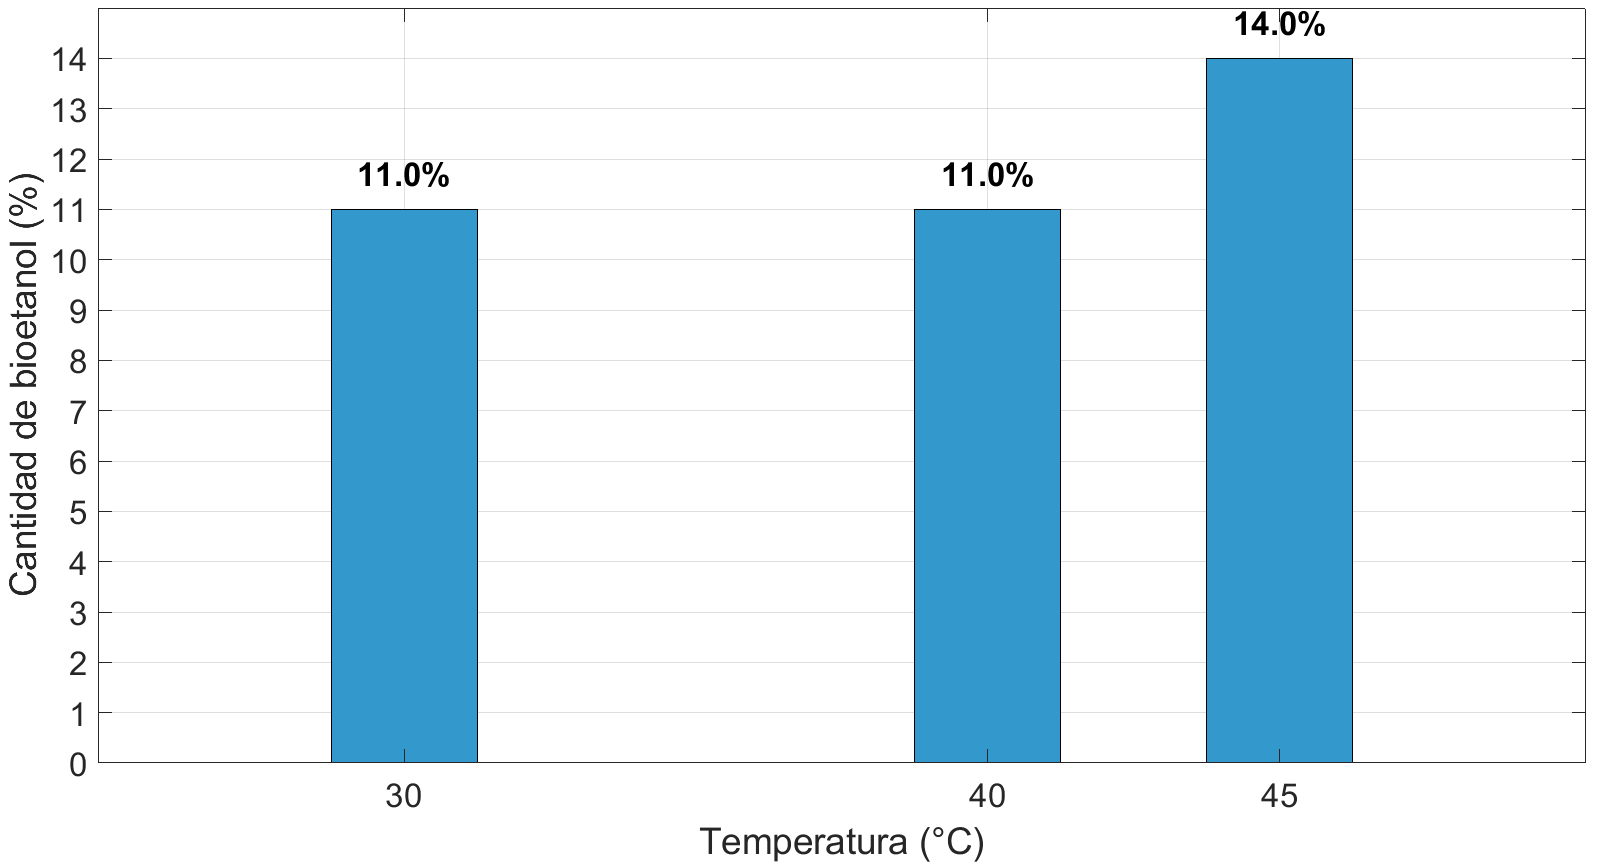
\includegraphics[width=\linewidth]{imagenes/biologico_TNUB}
					\caption{Producción de bioetanol con pretratamiento biológico con bagazo de caña  de TNUB}
					\label{fig:imagen1}
				\end{subfigure}
				\hfill % Espacio horizontal entre imágenes
				\begin{subfigure}[b]{0.49\textwidth}
					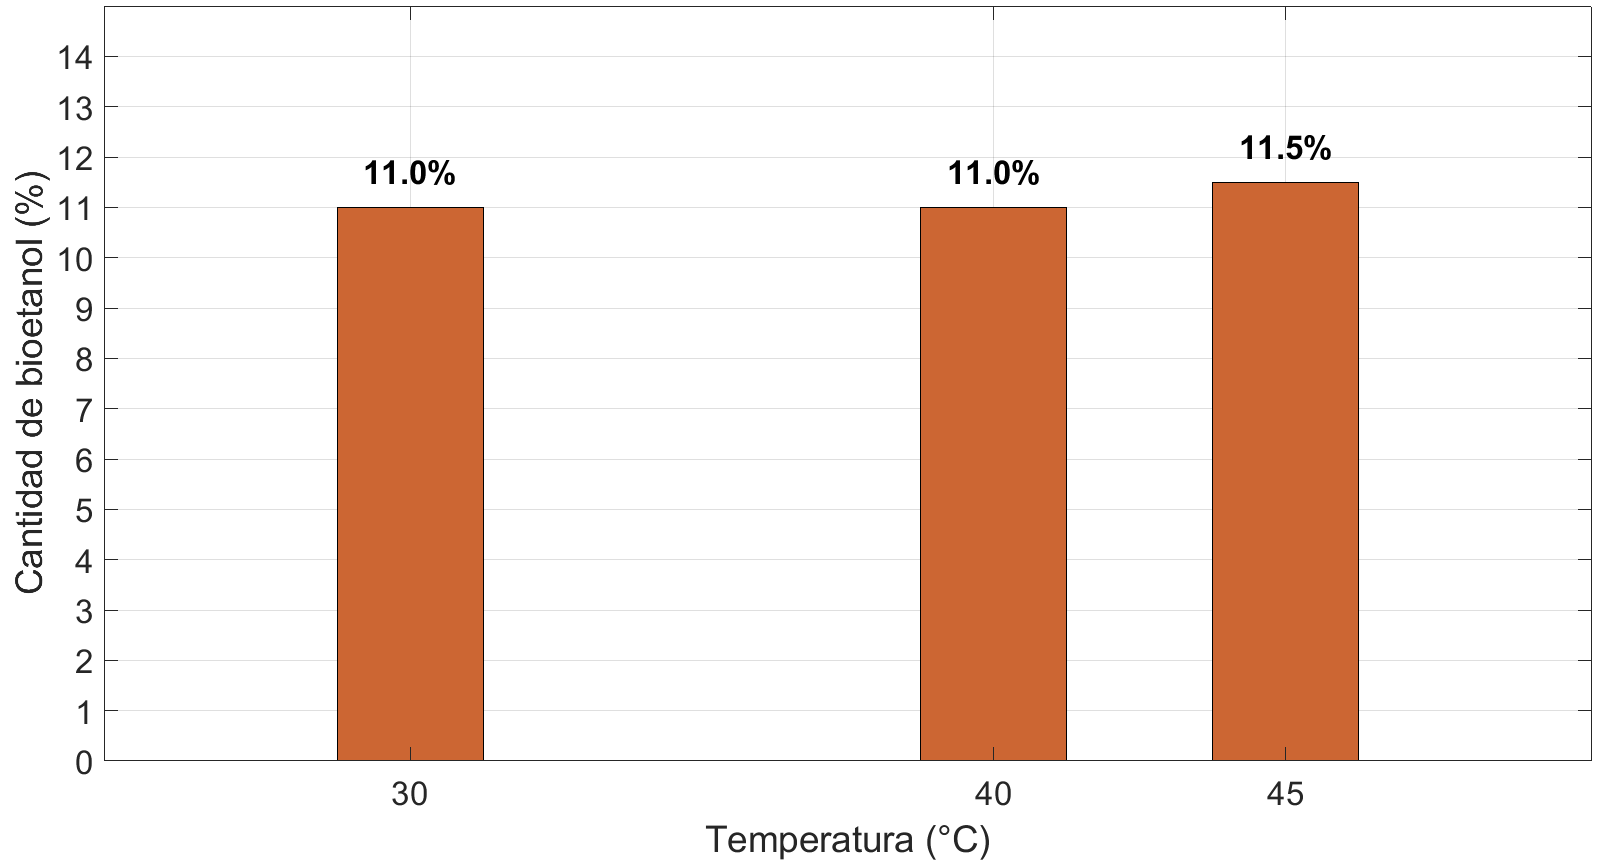
\includegraphics[width=\linewidth]{imagenes/biologico_11}
					\caption{Producción de bioetanol con pretratamiento biológico con bagazo de caña de 1 cm}
					\label{fig:imagen2}
				\end{subfigure}
				\caption{Producción de bioetanol con pretratamiento biológico.}
				\label{fig:pareja}
			\end{figure}

		
			
			
		
			Para el pretratamiento alcalino podemos observar que para un TNUB no hay cambios modificando la temperatura, sin embargo para 1 cm hay cambios significantes con una temperatura de 90°c
			
		
				\begin{figure}[ht]
				\centering
				\begin{subfigure}[b]{0.49\textwidth}
					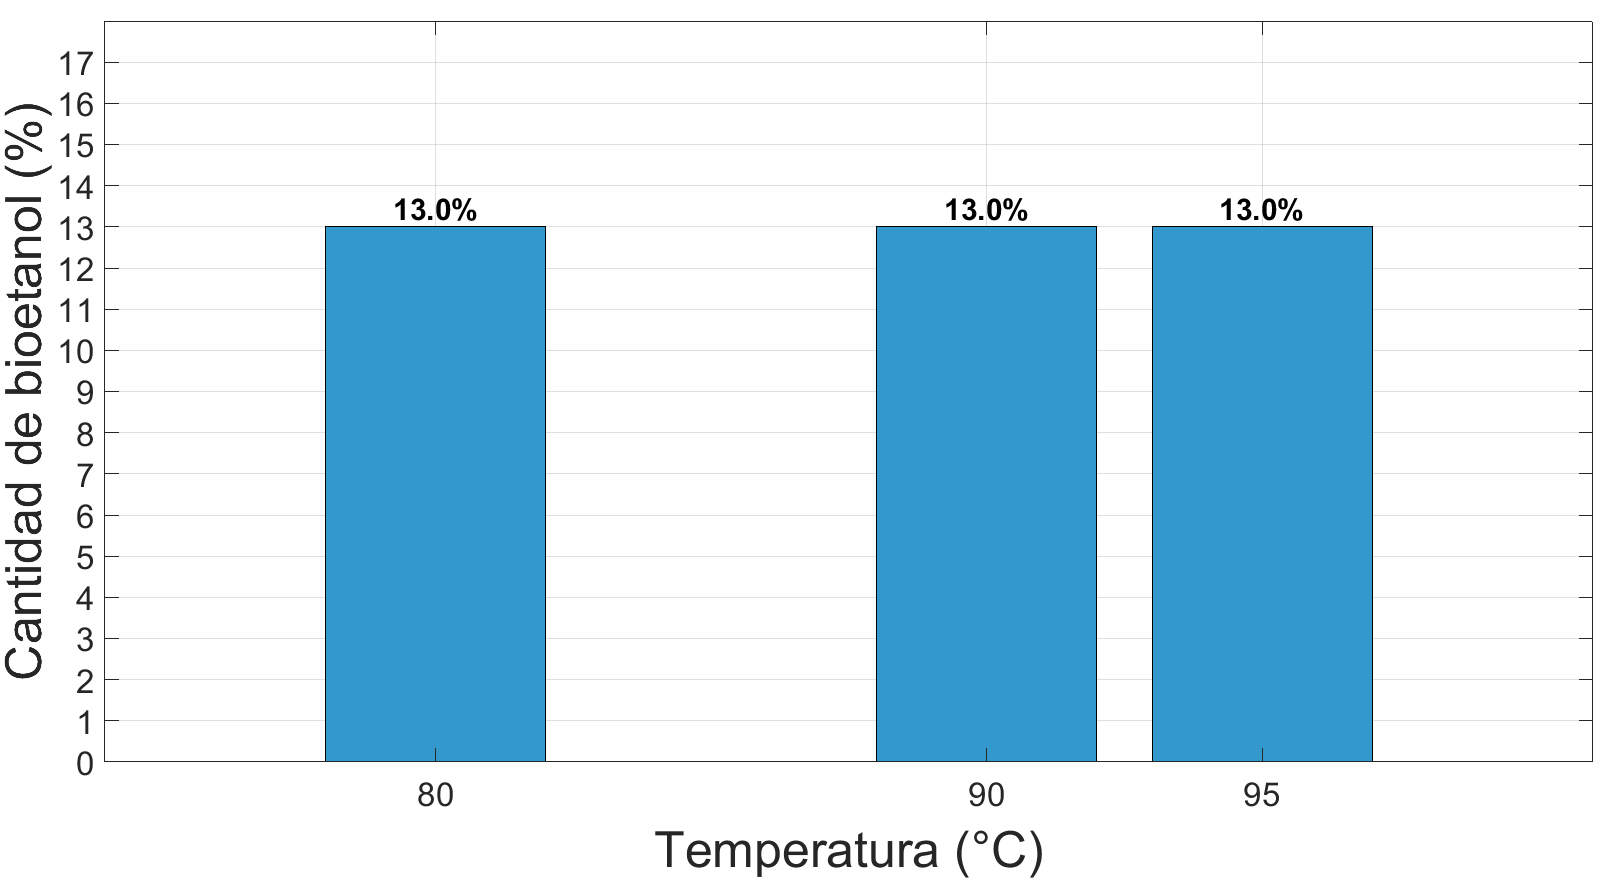
\includegraphics[width=\linewidth]{imagenes/alcalino_TNUB}
					\caption{Producción de bioetanol con pretratamiento alcalino con bagazo de caña  de TNUB}
					\label{bipoo}
				\end{subfigure}
				\hfill % Espacio horizontal entre imágenes
				\begin{subfigure}[b]{0.49\textwidth}
					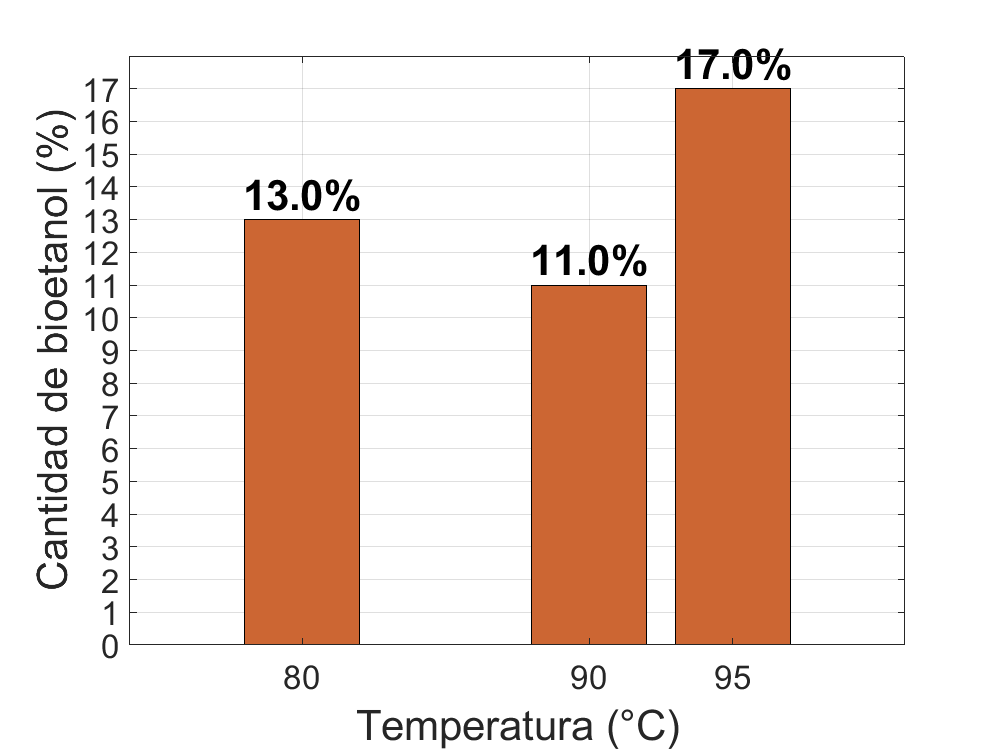
\includegraphics[width=\linewidth]{imagenes/alcalino_1cm}
					\caption{Producción de bioetanol con pretratamiento alcalino con bagazo de caña de 1 cm}
					\label{fig:imagen2}
				\end{subfigure}
				\caption{Producción de bioetanol con pretratamiento alcalino.}
				\label{fig:pareja}
			\end{figure}
			
			Se busca conocer cuanto consumo energético hubo en cada uno de los proceso por lo que a continuación se presenta mediante una grafica el promedio de la energia que se utilizo en esta etapa.
			
						\begin{figure} [H]
				\centering
				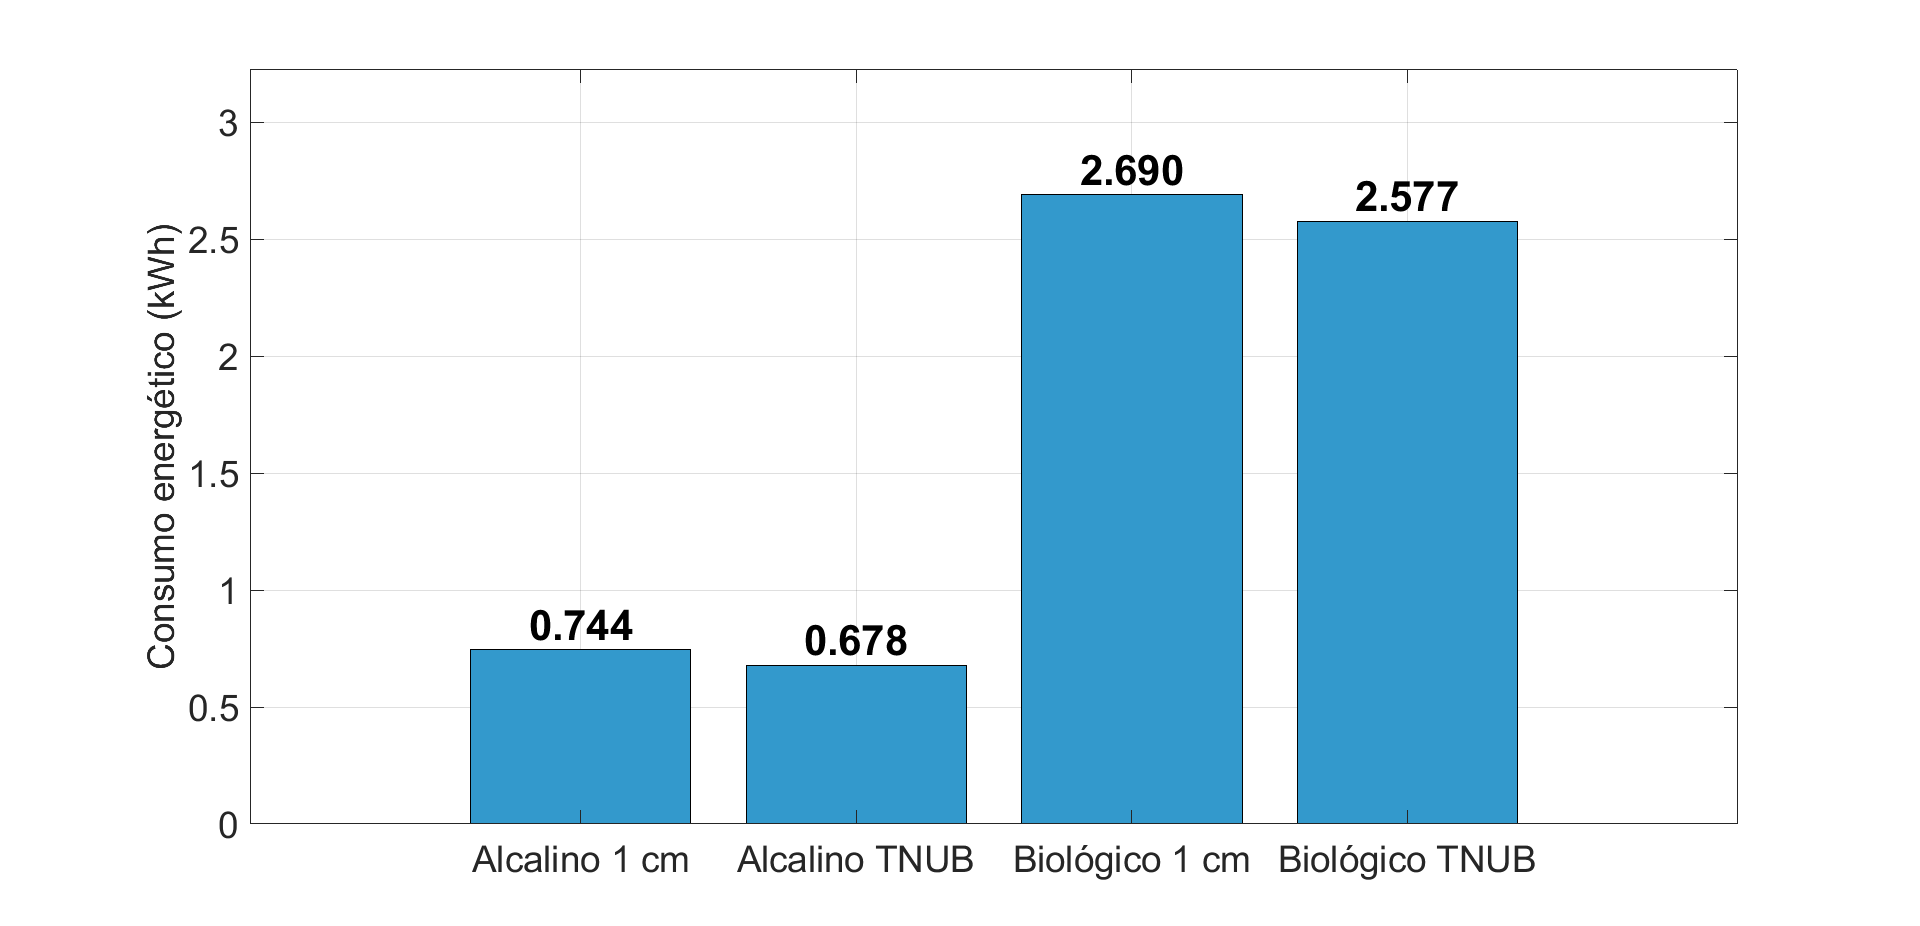
\includegraphics[width=16cm, height=7cm]{imagenes/consumoenergetico}
				\caption{Consumo energético para los dos tipos de pretratamiento. }
				\label{grafica}
			\end{figure}
			
			Gracias a la grafica podemos concluir que el pretratamiento biologico consume 3.7 veces mas energía que el pretratamiento biologico, sin embargo el costo por Kwh es muy pequeño, por lo que el impacto económico es menor.


\begin{figure} [H]
	\centering
	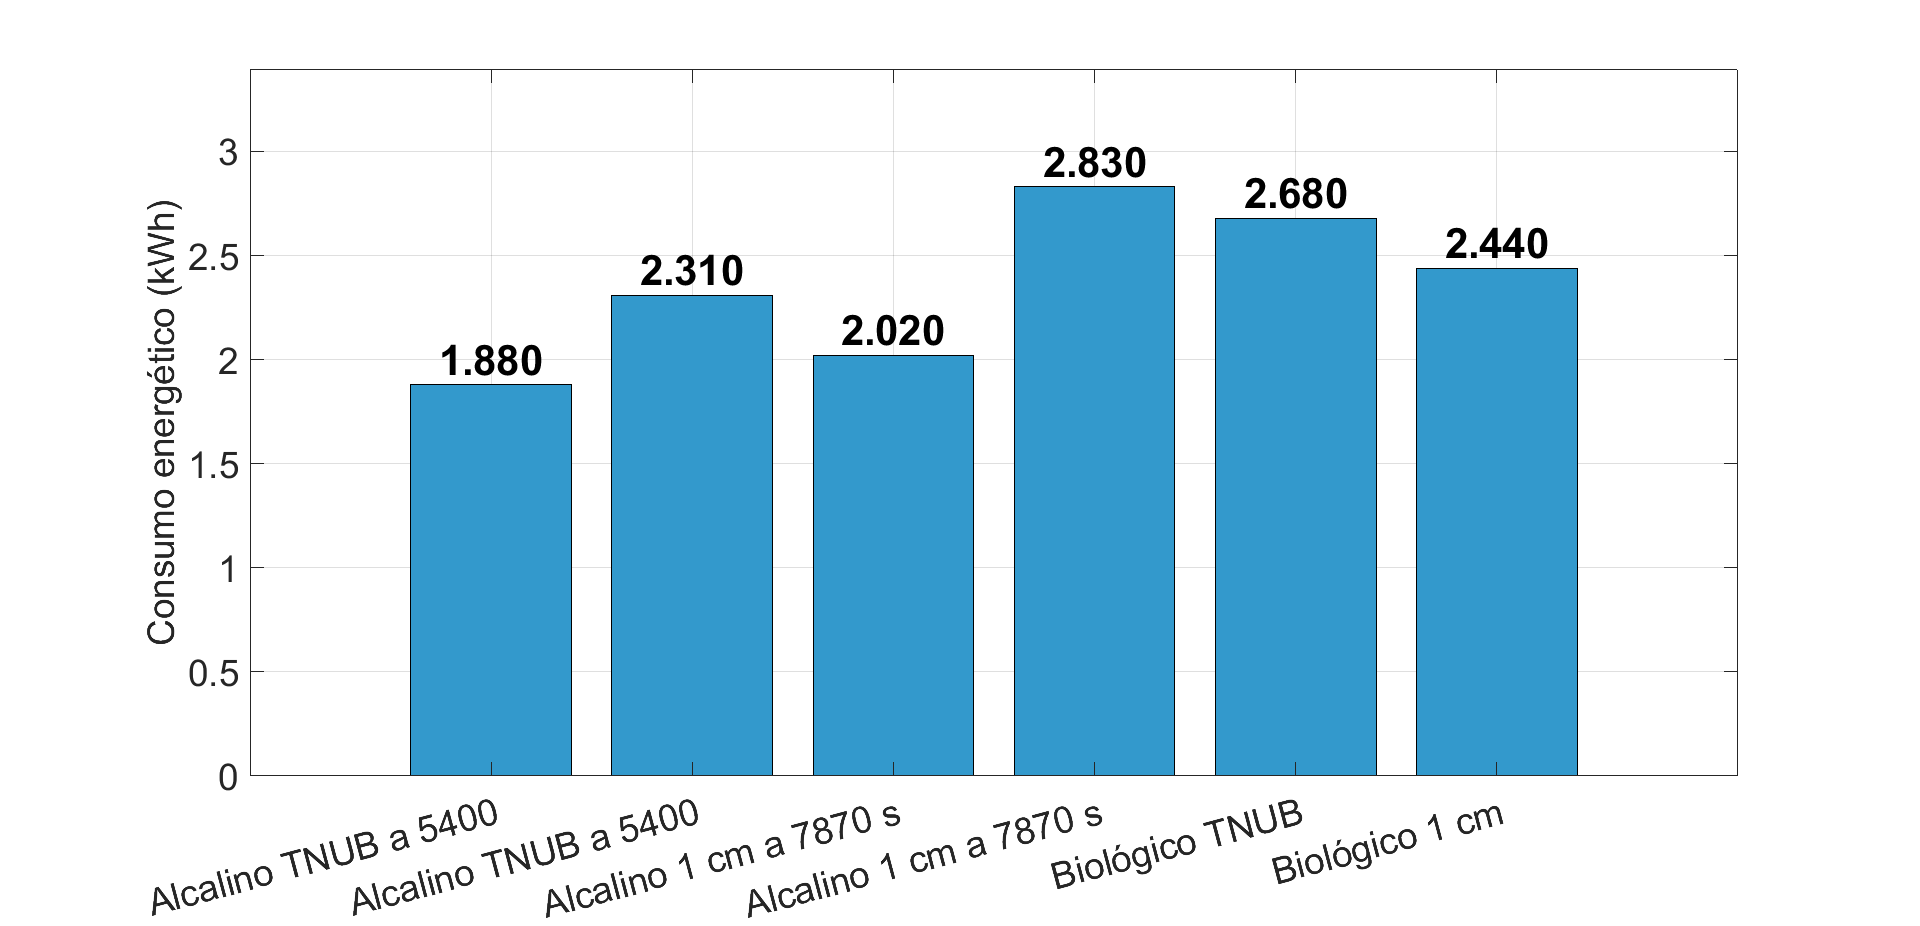
\includegraphics[width=16cm, height=7cm]{imagenes/CONSUMOENERGETICOSSF}
	\caption{Consumo energético para SSF. }
	\label{grafica}
\end{figure}


En la etapa de hidrólisis y fermentación en simultanea el margen de cambio en promedio del consumo energético es pequeño, esto puede deberse a la temperatura en el lugar
		\section{Conclusión}
		%\begin{itemize}
		Con respecto a lo mencionado anteriormente podemos concluir que en el pretratamiento biologico existe un cambio modificando el tamaño de partícula, así como la temperatura con mayor producción es de 45°.
		Para el pretratamiento alcalino podemos observar que un tiempo de  5400 s no presenta cambios en la producción de bioetanol, aun modificando el tamaño de partícula y la temperatura. Sin embargo un tamaño de partícula de 1 cm .
		
		
		
			%\item  Se podría proponer un sistema tolerante a fallas que tome en cuanta la variacion dentro del coeficiente de tranferencia de calor para saber cuando el equipoo se encuentra operando en optimas condiciones y cuando no lo esta haciendo. 
			
		%	\item 
			
		%\end{itemize}
		
		\newpage
	


	  
	   \bibliography{library}
	   
	   
		%\begin{appendix}
		%\section{Anexos}
	\newpage

% Anexos
%\cleardoublepage


%\begin{appendix}
%\section{Anexos}

%\begin{appendix}
		
\section*{Anexos}		
		
\newcounter{anexo}
\setcounter{anexo}{0}

% Para cada anexo:
\stepcounter{anexo}
\subsection*{A.\theanexo\ Bioetanol de segunda generación}
\addcontentsline{toc}{subsection}{A.\theanexo\ Bioetanol de segunda generación}
	

		los anexos son los siguientes
		\label{marco conceptual}
		
		
	%	\subsection{ Bioetanol de segunda generación}
		
		La producción de bioetanol de segunda generación utiliza como materia prima residuos agrícolas o desechos orgánicos, dependiendo asi de la infraestructura adecuada para obtener la producción de bioetanol. El proceso de producción de bioetanol de segunda generación no tiene una ruta estandarizada, por lo que debe adaptarse a la naturaleza de la materia prima \cite{melendez2022biotecnologia} (Melendez, J. R. 2022). El bioetanol de segunda generación se puede obtener con diferentes configuraciones: Sacarificación enzimática de la biomasa pretratada y la fermentación separadas, Sacarificación y fermentación simultáneas, sacarificación y co-fermentación simultáneas y bioproceso consolidado (gonzalez202).
		
	
		\subsection{ Definición de conceptos }
		
		
		Una parte  importante de la producción de bioetanol de segunda generación es conocer los conceptos, puntualmente los que forman parte del proceso, entre ellos se encuentran el etanol, la biomasa y mas 
		\subsubsection{Etanol}
		El etanol es un tipo de alcohol que en su mayoría es producido a partir de la  fermentación de las azucares fermentables, que se obtienen por microorganismos productores de etanol \cite{} (gonzales,2021).Considerado como un combustible ecológico, tipo de alcohol $\text{C}_2\text{H}_5\text{OH}$ (Alcohol etílico), que es obtenido a partir de materia lignocelulosa, puede ser utilizado como sustituto de gasolina por sus propiedades (Ballesteros, 2002).
		
		\subsubsection{Biomasa}
		
		\subsubsection{Bagazo de caña}
		El material es recuperado de la producción de azúcar, se obtiene después de un triturado después de obtener el jugo de la caña, este tipo de biomasa no es aprovechada. Esta biomasa tiene un 28\% en peso de la caña, y también, un 45\% de fibra, 2-3\% de sólidos insolubles y otro mismo porcentaje de sólidos solubles, finalmente la mitad de este material está conformado de agua \cite{olmo2015bagazo}.
		El bagazo representa el de mayor tonelaje y volumen de la producción de azúcar de caña, generando un promedio de 270 kg de bagazo por tonelada \cite{perez2022efecto}.
		
		\begin{figure}[h]
			\centering
			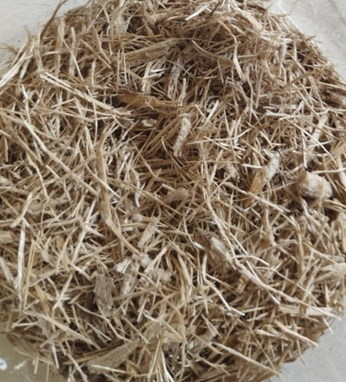
\includegraphics[width=0.4\linewidth]{imagenes/bagazo}
			\caption[Bagazo de caña]{}
			\label{fig:bagazo}
		\end{figure}
		
		\subsubsection{Lignocelulosa}
		
		Proveniente de la fotosíntesis, la lignocelulosa es uno de los componentes más abundante y principal de la biomasa, esta forma la pared celular de las plantas. Entre las plantas, la composición y porcentajes de lignocelulosa varían, dependiendo de la edad y etapa de crecimiento de las plantas \cite{cuervo2009lignocelulosa}.
		Es viable utilizar este material por su bajo costo, su alta disponibilidad y aprovechamiento variado, un ejemplo es en la industria de los materiales compuestos \cite{jara2022principales}.
		Ya que son viables, se han desarrollado usos alternativos para aprovechar este subproducto agroindustrial, utilizándolo en la creación de biocombustibles.
		La lignocelulosa está conformada por celulosa, hemicelulosa y lignina, siendo una fuente de carbono y energía renovable \cite{portalproduccon}. 
		
		\subsubsection{Pretratamiento}
		
		El pretratamiento es parte importante en el proceso de obtención del bioetanol de segunda generación,dado que el procesamiento de biomasa lignocelulósica complementa la hidrólisis enzimática y posibilita la obtención de altos rendimientos. Siendo necesario ya que la lignina en las paredes celulares en la planta crean barreras contra en ataque enzimático %\cite{riano2010produccion}.
		\newline 
		
		\begin{figure}[H]
			\centering
			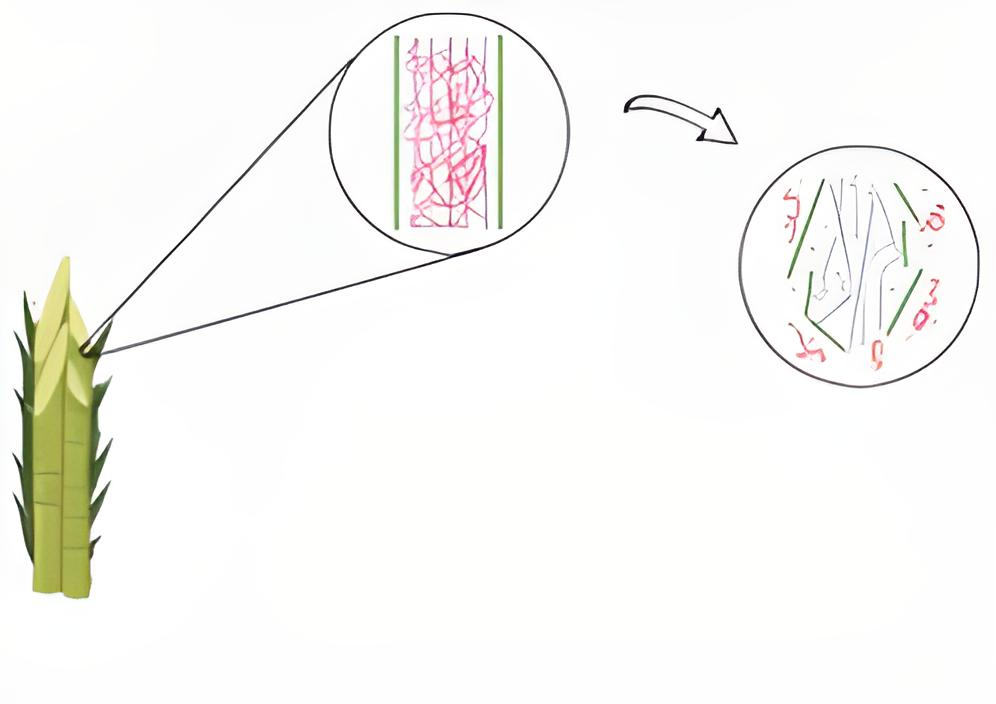
\includegraphics[width=0.4\linewidth]{imagenes/pretrata_1}
			\caption[Efecto del pretratamiento de biomasa ligno- celulósica]{}
			\label{fig:pretrata1}
		\end{figure}
		
		
		\subsubsection{Hidrólisis}
		También llamado despolimerización del material lignocelulósico. La biomasa con la dificultad de transformase químicamente  o biológicamente tiene el requisito de realizar una hidrólisis, entre mayor concentración de monosacáridos, mejor sera el rendimiento.La hidrólisis es un proceso que ayuda la formación de azucares siendo muy importante en la producción de etanol y en la obtención de otros productos. Existen distintos tipos de hidrólisis en la Tabla \ref{tipos de hidrolisis} se puede obtener mas información .
		
		\begin{table}[H]
			\centering  
			\caption{Tipos de hidrólisis }% \citep{ADITIYA2016631} }
			\label{tipos de hidrolisis}
		\begin{tabular}{  | c | c |}
			\hline \textbf{Tipo de hidrólisis} &\textbf{ Proceso y concepto}\\ \hline 
			Hidrólisis ácida   &   Explosión de CO2  \\ 
			
			&   Hidrólisis ácida \\ \hline 
			
			
			& Expolición de vapor\\
			&  Agua caliente \\ \hline
			Biológico & Bacterias \\
			&  Hongos \\ \hline
			Alcalino  & liquido iónico  \\
			& Hidrólisis alcalina \\ \hline
			Químico   & Ozonólisis\\
			&  Proceso con disolventes orgánicos\\
			& Oxidación húmeda \\ \hline
			Mecánico  & Trituración \\
			&  Pirólisis \\
			&  Microondas \\ \hline
			
		\end{tabular}
		\label{tipos de pretratamientos}
		\end{table}
		
		
		
		\begin{itemize}
		\item  Carga enzimática
		\end{itemize}
		
		Para la hidrólisis enzimática es necesario tomar la carga enzimática a utilizar en la prueba experimental, a carga enzimática se refiere a la cantidad de enzimas utilizadas en el momento de la experimentación, la cantidad de enzima esta dada en UPF (unidades papel filtro),  para obtener el valor en ml se utiliza la formula siguiente, obtenida de \cite{Arturo2022evaluacion}, donde necesitamos los UPF a utilizar y la carga de bagazo pretratado.
		
			\begin{equation}
			 ml = \left( \frac{0.37}{\text{UPF}} \right) \times \textit{cantidad de bagazo} 
			\end{equation}
		
		
		
		\subsubsection{Fermentación}
		La fermentación es un proceso bioquímico complejo, donde los microorganismos metabolizan azúcares y otros componentes para tener como resultado el bioetanol (escobar,2019), algunos de los microorganismos que pueden transformar son los hongos, bacterias, levaduras. Debido a la complejidad, a que es difícil de controlar y a las múltiples variables que afectan el proceso de fermentación se debe tener un entorno favorable. (rojas2021)
		Es un proceso que se realiza la hidrólisis de los polisacáridos convirtiéndolos en monosacáridos, todo esto en presencia de organismos fermentativos consumiendo los azúcares simples.
		
		
		
		
		\subsection{Configuraciones en la producción de bioetanol}	
		\subsubsection{Sacarificación enzimática de la biomasa pretratada y la fermentación separadas}
		
		El proceso de sacarificación enzimática y fermentación (SHF) se realiza por separado debido a que las temperatura que se tienen en las distintas fases son diferentes, en el caso de las enzimas hidrolíticas se tiene un promedio de 50°c, y una temperatura mas baja en el caso de la fermentación de 30°C-32°C. 
		La producción de biocombustible por etapas separadas es una de las técnicas mas antiguas, realizando un pretratado de enzimas para su hidrólisis y posteriormente una fermentación de la biomasa resultante  \cite{CHOUDHARY201682}.
		
		
		
		
		\subsubsection{Sacarificación y fermentación simultáneas}
		
		En el artículo \cite{CHOUDHARY201682} menciona que la sacarificación se realiza simultáneamente con la fermentación.
		La producción de etanol con microorganismo de importancia industrial como Saccharomyces cerevisiae (levaduras), no permite la utilización completa, este es incapaz de fermentar los azúcares. Se tiene la posibilidad de mantener la concentración de glucosa a un nivel bajo que permite una eficiente co-fermentación.
		%%%%%
		Este se lleva a acabo en un mismo contenedor, solucionando el problema de la utilización de productos para mayor producción de enzimas, siendo un problema limitante en la Sacarificación enzimática y fermentación (SHF). Mejorando la eficiencia de la sacarificación enzimática como el rendimiento de etanol. 
		Las enzimas hidrolíticas son adaptables al frío y las levaduras termófilas son importantes que se mantengan a temperatura ambiente \cite{CHOUDHARY201682}.
		
		\subsection{Proceso de obtención de bioetanol 2 G  utilizando una configuración SSF  }		
		Para la producción de bioetanol de segunda generación utilizando una configuración de dos etapas en conjunto, utilizando materia lignocelulósica se utilizan los pasos que menciona el diagrama de la Figura \ref{fig:diagrama-produccionssf}.
	
		\begin{figure}[H]
			\centering
			\includegraphics[width=0.6\linewidth]{imagenes/diagrama producciónssf}
			\caption{Diagrama donde menciona el proceso de bioetanol 2G}
			\label{fig:diagrama-produccionssf}
		\end{figure}
		
		
	Este diagrama menciona los pasos como el pre-pretratamiento, donde se realiza un clasificado de tamaño de materia lignocelulósico, así como una limpieza y un secado, posteriormente se realiza un pretratamiento donde rompe las barreras de la lignina y obteniendo como resultado una materia con azúcares fermentables . En cuanto a la hidrólisis y fermentación se toma la materia previamente pretratada y es puesta en una hidrólisis y fermentación y por ultimo se realiza una destilación.
		
		
		
		\subsection{Pretratamientos}
		En la Tabla \ref{tipos de pretratamientos} se listan los principales pretratamientos, cuya aplicación se reporta en diferentes investigaciones sobre la producción de bioetanol de segunda generación.% \citet{ADITIYA2016631} y \citet{Nasution_2022}
		ofrecen dos revisiones completas sobre pretratamientos de biomasa para la producción de bioetanol.
		
		\begin{table}[H]
		\centering  
		\caption{Tipos de pretratamiento }% \citep{ADITIYA2016631} }
		\begin{tabular}{  | p{5cm} | p{6.5cm} |}
		\hline\textbf{ Tipo de pretratamiento} & \textbf{ Método}\\ \hline 
		Ácido     & Percolación de amoníaco reciclado  \\ 
		&  Ácido diluido  \\
		&  Ácido concentrado \\
		&   Explosión de CO2  \\ 
		&   Hidrólisis ácida \\ \hline 
		Térmico   & Expolición de vapor\\
		&  Agua caliente \\ \hline
		Biológico & Bacterias \\
		&  Hongos \\ \hline
		Alcalino  & liquido iónico  \\
		& Hidrólisis alcalina \\ \hline
		Químico   & Ozonólisis\\
		&  Proceso con disolventes orgánicos\\
		& Oxidación húmeda \\ \hline
		Mecánico  & Trituración \\
		&  Pirólisis \\
		&  Microondas \\ \hline
		
		\end{tabular}
		\label{tipos de pretratamientos}
	\end{table}


\subsubsection{Pretratamiento alcalino}

El pretratamiento con NaOH es uno de los más utilizados en pretratamientos alcalinos,  ya que genera un incremento en la hidrólisis \cite{espinosa2021pretratamiento}, en cambio, producen una perdida de celulosa y hemicelulosa, generando una menor producción de azúcares y bioetanol.
El pretratamiento utiliza, hidróxido sódico, amoniaco o cal, generando menos inhibidores, lo cual obtiene una mayor deslignificación en comparación con tratamiento con ácidos %\cite{valles2022estudio}.

\subsubsection{Pretratamiento biológico }

Existen pretratamientos biológicos en los que comúnmente se usan microorganismos, hongos, y enzimas que promueven la degradación de la lignina. El uso de hongos en este tipo de procesos ayuda a descomponer la lignina. En general, estos pretratamientos tienen bajo consumo energético en su implementación, %\citep{Gonzalez2018desarrollo}. 




\subsection{Reactores tipo Batch }





%%%%%%%%%%%%%%%%%%%%%%%%%%%%%%%%%%%%%%%%%%%%%%%%%%%%%%%%%%%%%%%%%%%%%%%%%%%%%%%%%%%%%%%%%%%%%%%%%%%%%%%%%%%%%%%%%%%%%%%%%%%%%%%%%%%%%%%%%%%%%%%%%%%%%%%%%%%%%%%%%%%%%%%%%%%%%%%%%%%%%%%%%%%%%%%%%%%%%%%%%%
	% \newline
	
	
		\section{Estado del arte}

	\label{Estado del arte}
El estado del arte es una minuciosa búsqueda de información referente a los avances científicos y tecnológicos de la producción de bioetanol de segunda generación, principalmente utilizando etapas juntas en el proceso. Esta revisión muestra algunos avances en la etapa de pretratamientos en el proceso de producción.

El pretratamiento es un paso muy importante para la producción de bioetanol de segunda generación, algunos de los pretratamientos que existen son: Ácido, Térmico, Biológico, alcalino, Químico, Mecánico (\cite{ADITIYA2016631}).
El pretratamiento con NaOH es uno de los más utilizados como pretratamientos alcalinos, este promueve la hidrólisis \cite{espinosa2021pretratamiento}. Una desventaja de este es la pérdida de celulosa y hemicelulosa, y la reducción de azúcares y bioetanol.
En general, el pretratamiento alcalino genera menos inhibidores y favorece la deslignificación, en comparación con tratamiento con ácidos, según \cite{valles2022estudio}. 

También hay pretratamientos biológicos en los que comúnmente se usan microorganismos, hongos, y enzimas que promueven la degradación de la lignina. El uso de hongos en este tipo de procesos ayuda a descomponer la lignina. En general, estos pretratamientos tienen bajo consumo energético en su implementación, \cite{Gonzalez2018desarrollo}.  

\subsection{Tecnología de bioetanol de segunda generación.}




\subsection{Pretratamientos.}









\subsubsection{Pretratamiento Alcalino}

El pretratamiento alcalino consiste en sumergir un material lignocelulósico en una solución alcalina bajo ciertas condiciones de temperatura, concentración, y tiempo de tratamiento. Los álcalis más usados son hidróxido de sodio (NaOH), de potasio (KOH) o de amonio (NH$_4$OH). Estos compuestos rompen los enlaces entre la lignina y los carbohidratos, o solubilizan parcialmente la lignina \cite{Galbe2012}.
% REF. % Galbe, M., & Zacchi, G. (2012). Pretreatment: The key to efficient utilization of lignocellulosic materials. Biomass and Bioenergy, 46, 70?78.
Enseguida se describen algunas investigaciones sobre pretratamientos alcalinos como medio para favorecer la hidrólisis enzimática de la biomasa, que para la actual revisión es el bagazo de caña.

\cite{Nasution_2022} presentó una revisión de los pretratamientos más usados en los últimos años. Como pretratamiento alcalino se destaca el uso del NaOH. Comúnmente se recomienda manejar una concentración al 2 \% de NaOH, una relación de agua destilada de 1:10 solido-liquido, y una temperatura de operación de 80 °C, así como un tiempo de tratamiento de 2h.

En un estudio afin, \cite{Arturo2022evaluacion} utilizó como biomasa bagazo de caña para producir bioetanol con dos modos diferentes de producción: sacarificación enzimática y fermentación en etapas separadas (SHF), y Sacarificación y fermentación simultáneas (SSF). Se probaron 4 tipos de pretratamientos de la materia prima, entre estos se aplicó un pretratamiento alcalino usando como base NaOH al 2 \% p/v y una carga de bagazo del 4\% p/v. El pretratamiento se llevó a cabo a 97°C durante un tiempo de 90 minutos. Al finalizar este tiempo, la biomasa tratada se acondicionó mediante etapas de enjuagado, filtrado y secado para después ser procesada por cada modo de producción, SHF o SSF. Comparando el porcentaje de alcohol obtenido a partir de cada proceso (SHF o SSF), se concluyó que el proceso SHF obtuvo un producto más concentrado, con 15 \% de alcohol, mientras que el producto del proceso SSF tenía un contenido de alcohol menor de 11 \%. En contra parte se concluyó que el proceso SSF reduce en un 80\% el tiempo consumido por el proceso SHF.

\textbf{Conclusión}\\



\subsubsection{Pretratamiento Biológico}





%%%%%%%%%%%%%%%%%%%%%%%%%%%%%%%%%%%%%%%%%%%%%%%%%%%%%%%%%%%%%%%%%%%%%%%%%%%%%%%%%%%%%%%%%
\subsubsection{Otros pretratamientos} 



\textbf{Pretratamiento ácido} 

El pretratamiento ácido se realiza impregnando en un ácido diluido el material lignocelulósico. Comúnmente se usan ácidos minerales como el ácido sulfúrico (H$_2$SO$_4$), que fragmenta los componentes de la biomasa en moléculas más pequeñas \cite{Galbe2012}. Como ejemplo se citan los siguientes estudios. %%%%%pendiente 
Regresando al trabajo de \cite{Arturo2022evaluacion}, entre los pretratamientos que se presentaron está también uno con ácido sulfúrico ($H_2 S0_4$) y agua destilada. Para este caso se efectuaron experimentos con 3 porcentajes de carga de biomasa (4\%, 6\%, 8\%) a temperatura máxima de 97°C y con duración de 60 minutos. Para el proceso SSF se obtuvo un producto con 7 \% de alcohol, es decir un rendimiento menor que el obtenido con el pretratamiento alcalino desarrollado en el mismo trabajo para bagazo de caña.

Otro trabajo sobre producción de bioetanol con bagazo de caña  pretratado con ácido es el de \cite{TANTAYOTAI2022102499}, quienes compararon la efectividad de dos ácidos, uno orgánico y otro mineral. Como resultado, se concluyó que el pretratamiento con ácidos orgánicos fue más efectivo porque se logró mayor rendimiento.

%%%%%
\cite{rojas2010analisis} y sus colaboradores también expusieron sus resultados para 3 pretratamientos de bagazo de caña, incluido uno ácido. Su objetivo fue comparar el impacto ambiental de los tres pretratamientos. Al igual que en los trabajos antes citados, el pretratamiento se hizo con H$_2$SO$_4$. Se usó el ácido al 1.5 \% en peso y se procesó a 160°C. Se obtuvo como resultado la degradación del 90\% de la hemicelulosa y una completa solubilidad de la lignina. Después del pretratamiento se efectuaron la fermentación, la destilación y la purificación del producto. La etapa de SSF se concluyó con un rendimiento de 85 \% de la sacarificación y fermentación de la celulosa, mientras que el rendimiento del proceso SHF fue de 75 \%  con respecto a la fermentación de azucares. Finalmente, se concluyó que al comparar los tres tipos de pretratamientos efectuados, el ácido no se encuentra entre los mas contaminantes.

%%revisar

\textbf{Pretratamiento térmico } 


Regresando al trabajo de \cite{rojas2010analisis}, otro de los pretratamiento probados para el bagazo de caña fue un pretratamiento térmico en condiciones de temperaturas y presiones elevadas, de 220 °C y 22.9 atm. Al analizar los niveles de contaminación de los pretratamientos, se concluyó que dada la cantidad de energía que se requiere para llegar a altas temperaturas, el pretratamiento térmico resultó el más contaminante.

El trabajo de \cite{MOONSAMY2022115675} tuvo como objetivo lograr una producción autosustentable, creando distintos escenarios. Un aspecto escencial de su análisis fue explorar la vialidad de combinar procesos de primera y segunda generación a partir de melazas y material lignocelulósico provenientes de la caña de azúcar. El pretratamiento propuesto fue el de explosión de vapor. Este consiste en hacer pasar una corriente líquida de hemicelulosa con una parte solida de celulosa y lignina. Posteriormente, dependiendo del escenario se realizó una SSF o una SHF. La conclusión fue que la ventaja del proceso combinado es su factibilidad económica, el reto es evitar la inhibición o supresión de la glucosa.
%%%%%%%%%%%%%%%%%%%%%%%%%%%%%%%%%%%%%%%%%%%%%%%%%%%%%%%%%%%%%%%%%%%%%%%%%%%%%%%%%%%%%%%%%

\subsection{Configuraciones en la producción de bioetanol}



\subsubsection{Sacarificación enzimática de la biomasa pretratada y la fermentación separadas} 

%%% otros
En el artículo de \cite{Gomes2022analisis} se analizaron tres configuraciones para fermentación de bagazo de caña, ante diferentes condiciones de operación en modo por etapas separadas. Con un primer análisis se evaluó la influencia de la humedad, comparando la efectividad del proceso para humedades de la biomasa del 40\% y 60\%. Se concluyó que con menor humedad, el rendimiento de bioetanol aumenta. En un segundo análisis se evaluó el efecto de la velocidad de dilución durante la fermentación. El resultado fue que a mayor velocidad, el producto tiene mayor concentración de etanol. Por último se implementó una SSF, en la que se alcanzó un rendimiento bioetanol/bagazo del 12.5\%. 

\subsubsection{Sacarificación y fermentación simultáneas} 

\subsection{Producción de bioetanol de segunda generación en reactores tipo Batch}



		
%	\end{appendix}
	
	
	\section{Diseño del control de temperatura}
	
	\label{diseño del control de temp}
	
	
	
	\subsection{Respuesta de la planta aplicando una Señal PRBS}
	
	
	La señal PRBS entra  mediante la salida PWM del arduino a un convertidor, pasando después a la resistencia como se muestra en el diagrama de la Figura \ref{ diagrama_prbs}
	
	\begin{figure}[h!]
		\centering
		\includegraphics[width=.4\linewidth]{imagenes/diagrama_PRBS}
		\caption{Señal PRBS. }
		\label{ diagrama_prbs}
	\end{figure}
	
	En el reactor se mide mediante los sensores termopar k  la temperatura, esta temperatura ingresando la señal PWM tiene la forma siguiente como lo muestra la Figura \ref{ Temperatura_con PRBS}
	
	\begin{figure}[h!]
		\centering
		\includegraphics[width=.8\linewidth]{imagenes/temperatura con prbs}
		\caption{Comportamiento de la temperatura dentro del reactor con señal de entrada PRBS }
		\label{ Temperatura_con PRBS}
	\end{figure}
	
	
	Como se puede observar en la imagen la temperatura sufre de variaciones,  sin embargo dichas variaciones ayudaran a obtener la identificación del sistema con mayor precisión de la planta.
	Para obtener la temperatura neta del sistema , es decir la temperatura sin la influencia de la temperatura ambiente se resta la temperatura ambiente dentro del laboratorio menos la temperatura dentro del biorreactor.
	
	\begin{figure}[h!]
		\centering
		\includegraphics[width=.7\linewidth]{imagenes/temp_neta}
		\caption{Comportamiento de la temperatura sin la temperatura ambiente dentro del laboratorio. }
		\label{ Temperatura neta_con PRBS}
	\end{figure}
	
	La gráfica de la Figura \ref{ Temperatura neta_con PRBS} muestrala temperatura dentro del reactor 
	
	
	
	\subsection{Identificación del sistema de la planta}	
	
	Se necesita un sistema que modele el comportamiento de la temperatura de la planta, por lo que se realizaron técnicas de identificación, como es el caso de la técnica OE donde se obtiene el sistema 
	
	
	\begin{equation}
		G(s) = \frac{0.0005369 \, s^2 + 0.0003022 \, s + 8.207 \times 10^{-5}}{s^3 + 0.3314 \, s^2 + 0.0002728 \, s + 2.707 \times 10^{-7}}
	\end{equation}
	
	Esta función de transferencia tiene respuesta como se muestra en la siguiente figura \ref{fig:identificacion}, este sistema es de tercer orden
	
	
	\begin{figure} [h!]
		\centering
		\includegraphics[width=0.8\linewidth]{imagenes/identificacion}
		\caption{}
		\label{fig:identificacion}
	\end{figure}
	Para observar el comportamiento del sistema se puede ver los polos y ceros del sistema en la figura \ref{polos y ceros}
	
	\begin{figure} [h!]
		\centering
		\includegraphics[width=1\linewidth]{imagenes/Polos y ceros}
		\caption{}
		\label{polos y ceros}
	\end{figure}
	\newpage
	%%%%%%%%%%%%%%%%%%%%%%%%%%%%%%%%%%%%%%%%%%%%%%%%%%%%%%%%%%%%

	\subsection{Control PID}
	
	
	
	Un control PID puede ser calculado con la siguiente ecuación 
	
	\begin{equation}
		C(t) = K_p \, e(t) + K_i \int e(t) \, dt + K_d \frac{d e(t)}{dt}
	\end{equation}
	Para el control PID se utilizo la herramienta de MATLAB que tiene por nombre PID TUNER (Transfer function Based)
	
	\begin{figure}[h!]
		\centering
		\includegraphics[width=0.7\linewidth]{imagenes/pid tuner}
		\caption{Ventana de la herramienta PID Tuner}
		\label{fig:pid-tuner}
	\end{figure}
	
	Obteniendo como resultado los valores de cada variable del controldador PID:
	\begin{equation}
		P=0.00724555643948787 
	\end{equation}
	
	\begin{equation}
		I=9.60342545392904 X 10^{-07}
	\end{equation}
	
	\begin{equation}
		D=5.63241452981354
	\end{equation}
	
	Realizando un ajuste a los valores de la planta obteniendo como nuevos valores lo siguiente
	
	\begin{equation}
		P=0.19779
	\end{equation}
	
	\begin{equation}
		I=2.835 X 10^{-04}
	\end{equation}
	
	\begin{equation}
		D=-1.72
	\end{equation}
	
	Con estos valores se observa el control en las variables en el reactor, utilizando la herramienta MATLAB como lo muestra la figura \ref{sistema simulado}
	
	\begin{figure}[H]
		\centering
		\includegraphics[width=0.8\linewidth]{imagenes/sistema_controlado}
		\caption{Sistema simulado con control a 90 °C}
		\label{sistema simulado}
	\end{figure}
	
  En cada paso de la producción de bietanol se realizaron diseños de control para la temperatura, por lo que en la tabla se presentan los valores para cada parte de control.
	 
	
	
	\begin{table}[H]
		\centering
		\caption{Valores para el control de temperatura en pretratamiento y SSF}
		\begin{tabular}{|l|l|l|l|}
			\hline
			Variables & Pretratamiento Bilógico & Pretratamiento alcalino & SSF \\ \hline
			P & 0.5 & 0.19779 & 0.197 \\ \hline
	    	I & $2 x10^-9 $ & $2.835 x10^-4 $ & $2.8 x10^-8 $ \\ \hline
			D & 1.6 & -1.72 & -1.7 \\ \hline
\end{tabular}
\label{tabla_control}
\end{table}
	
	
	
	
	
	\end{document}